% -*- Mode:TeX -*-

%% IMPORTANT: The official thesis specifications are available at:
%%            http://libraries.mit.edu/archives/thesis-specs/
%%
%%            Please verify your thesis' formatting and copyright
%%            assignment before submission.  If you notice any
%%            discrepancies between these templates and the 
%%            MIT Libraries' specs, please let us know
%%            by e-mailing thesis@mit.edu

%% The documentclass options along with the pagestyle can be used to generate
%% a technical report, a draft copy, or a regular thesis.  You may need to
%% re-specify the pagestyle after you \include  cover.tex.  For more
%% information, see the first few lines of mitthesis.cls. 

%\documentclass[12pt,vi,twoside]{mitthesis}
%%
%%  If you want your thesis copyright to you instead of MIT, use the
%%  ``vi'' option, as above.
%%
%\documentclass[12pt,twoside,leftblank]{mitthesis}
%%
%% If you want blank pages before new chapters to be labelled ``This
%% Page Intentionally Left Blank'', use the ``leftblank'' option, as
%% above. 

\documentclass[12pt,twoside,singlespace]{mitthesis}
\usepackage{lgrind}
%% These have been added at the request of the MIT Libraries, because
%% some PDF conversions mess up the ligatures.  -LB, 1/22/2014
\usepackage{tikz-feynman}
\tikzfeynmanset{/tikzfeynman/warn luatex = false}
\usepackage{hyperref}
\usepackage{graphicx}
\usepackage{floatrow}
\usepackage{xspace}
\usepackage{xcolor}
\usepackage{cmap}
\usepackage[T1]{fontenc}
\usepackage{multirow}
\usepackage{textcomp}
\usepackage{siunitx}
\usepackage{rotating}
\usepackage[fleqn]{amsmath}
\usepackage{amssymb}
\usepackage{nonfloat}
\usepackage{titlesec}
\pagestyle{plain}
%\newcommand{\tw}{\ensuremath{tW}}
\newcommand{\dyee}{\ensuremath{Z/\gamma^*\to e^+e^-}}
\newcommand{\dymm}{\ensuremath{Z/\gamma^*\to\mu^+\mu^-}}
\newcommand{\dytt}{\ensuremath{Z/\gamma^*\to\tau^+\tau^-}}
\newcommand{\dyll}{\ensuremath{Z/\gamma^*\to\ell^+\ell^-}}
\newcommand{\WW}{\ensuremath{\W^+\W^-}}
\newcommand{\Lep}{\ensuremath{\ell}}
\newcommand{\mll}{\ensuremath{m_{\Lep\Lep}}}
\newcommand{\ptvecmiss}{\ensuremath{{\vec p}_{\mathrm{T}}^{\kern1pt\textrm{miss}}}\xspace}
\newcommand{\CLs}{\ensuremath{CL_\mathrm{s}}}
\newcommand{\CLb}{\ensuremath{CL_\mathrm{b}}}
\newcommand{\CLsb}{\ensuremath{CL_\mathrm{s+b}}}

\newcommand{\GeV}{\ensuremath{\mathrm{Ge\kern -0.1em V}}}
\newcommand{\TeV}{\ensuremath{\mathrm{Te\kern -0.1em V}}}
\newcommand{\TeVcc}{\ensuremath{\,\mathrm{Te\kern -0.1em V\!/c}^2}}
\newcommand{\GeVcc}{\ensuremath{\,\mathrm{Ge\kern -0.1em V\!/c}^2}}
\newcommand{\MeVcc}{\ensuremath{\,\mathrm{Me\kern -0.1em V\!/c}^2}}
\newcommand{\GeVc}{\ensuremath{\mathrm{Ge\kern -0.1em V}\!/c}}
\newcommand{\nanob}{\mbox{{\rm ~nb}~}}
\newcommand{\fb}{\ensuremath{\mathrm{fb}}}
\newcommand{\pb}{\ensuremath{\mathrm{pb}}}
\newcommand{\ifb}{\ensuremath{\mathrm{fb^{-1}}}}
\newcommand{\ipb}{\ensuremath{\mathrm{pb^{-1}}}}
\newcommand{\grad}{\ensuremath{^{\circ}}}
%
% Special user made math symbols
%
\newcommand{\lsim}{\raisebox{-1.5mm}{$\:\stackrel{\textstyle{<}}{\textstyle{\sim}}\:$}}
\newcommand{\gsim}{\raisebox{-1.5mm}{$\:\stackrel{\textstyle{>}}{\textstyle{\sim}}\:$}}

% particles

\newcommand{\pipm}{\ensuremath{\pi^{\pm}}}
\newcommand{\pizero}{\ensuremath{\pi^{0}}}
\newcommand{\Hi}{\ensuremath{\mathrm{H}}}
\newcommand{\V}{\ensuremath{\mathrm{V}}}
\newcommand{\W}{\ensuremath{\mathrm{W}}}
\newcommand{\Wjets}{\ensuremath{\mathrm{W+jets}}}
\newcommand{\Zjets}{\ensuremath{\mathrm{Z+jets}}}
\newcommand{\Wt}{\ensuremath{\mathrm{Wt}}}
\newcommand{\Wstar}{\ensuremath{\mathrm{W}^{*}}}
\newcommand{\Wparenthesisstar}{\ensuremath{\mathrm{W}^{(*)}}}
%\newcommand{\Z}{\ensuremath{\mathrm{Z}}}
\newcommand{\Zstar}{\ensuremath{\mathrm{Z}^{*}}}
\newcommand{\Wpm}{\ensuremath{\W^{\pm}}}
\newcommand{\ZZ}{\ensuremath{\Z\Z}}
\newcommand{\WZ}{\ensuremath{\W\Z}}
\newcommand{\El}{\ensuremath{\mathrm{e}}}
\newcommand{\Elp}{\ensuremath{\mathrm{e}^{+}}}
\newcommand{\Elm}{\ensuremath{\mathrm{e}^{-}}}
\newcommand{\Elpm}{\ensuremath{\mathrm{e}^{\pm}}}
\newcommand{\Elmp}{\ensuremath{\mathrm{e}^{\mp}}}
\newcommand{\M}{\ensuremath{\mu}}
\newcommand{\Mp}{\ensuremath{\mu^{+}}}
\newcommand{\Mm}{\ensuremath{\mu^{-}}}
\newcommand{\Mpm}{\ensuremath{\mu^{\pm}}}
\newcommand{\Mmp}{\ensuremath{\mu^{\mp}}}
\newcommand{\Tau}{\ensuremath{\tau}}
\newcommand{\Nu}{\ensuremath{\nu}}
\newcommand{\Nubar}{\ensuremath{\bar{\nu}}}
\newcommand{\Lepp}{\ensuremath{\ell^{+}}}
\newcommand{\Lepm}{\ensuremath{\ell^{-}}}
\newcommand{\Lprime}{\ensuremath{\Lep^{\prime}}}
\newcommand{\Prot}{\ensuremath{\mathrm{p}}}
\newcommand{\Pbar}{\ensuremath{\bar{\mathrm{p}}}}
\newcommand{\PP}{\Prot\Prot}
\newcommand{\PPbar}{\Prot\Pbar}
%\newcommand{\ttbar}{\ensuremath{\mathrm{t}\bar{\mathrm{t}}}}
\newcommand{\qq}{\ensuremath{\mathrm{q}\mathrm{q}}}
\newcommand{\bbbar}{\ensuremath{\mathrm{b}\bar{\mathrm{b}}}}
\newcommand{\Wtb}{\ensuremath{\W\mathrm{t}\mathrm{b}}}
\newcommand{\Top}{\ensuremath{\mathrm{t}}}
\newcommand{\Bot}{\ensuremath{\mathrm{b}}}
\newcommand{\Atop}{\ensuremath{\bar{\mathrm{t}}}}
\newcommand{\Abot}{\ensuremath{\bar{\mathrm{b}}}}
\newcommand{\WH}{\ensuremath{\W\Hi}}
\newcommand{\ZH}{\ensuremath{\Z\Hi}}
% arrow
\newcommand{\To}{\ensuremath{\rightarrow}}

% masses
\newcommand{\mHi}{\ensuremath{m_{\mathrm{H}}}}
\newcommand{\mW}{\ensuremath{m_{\mathrm{W}}}}
\newcommand{\mZ}{\ensuremath{m_{\mathrm{Z}}}}
\newcommand{\mt}{\ensuremath{m_{T}}}

% kinematics
\newcommand{\pt}{\ensuremath{p_\mathrm{T}}}
\newcommand{\ptveto}{\ensuremath{\pt^\mathrm{veto}}}
\newcommand{\ptl}{\ensuremath{p_\perp^{\Lep}}}
\newcommand{\ptlmax}{\ensuremath{p_{\mathrm{T}}^{\Lep,\mathrm{max}}}}
\newcommand{\ptlmin}{\ensuremath{p_{\mathrm{T}}^{\Lep,\mathrm{min}}}}
\newcommand{\Et}{\ensuremath{E_\mathrm{T}}}
\newcommand{\met}{\ensuremath{\Et^{\mathrm{miss}}}}
\newcommand{\delphill}{\ensuremath{\Delta\phi_{\Lep\Lep}}}
\newcommand{\deletall}{\ensuremath{\Delta\eta_{\Lep\Lep}}}
\newcommand{\delphimetl}{\ensuremath{\Delta\phi_{\met\Lep}}}
\newcommand{\delR}{\ensuremath{\Delta R}}
\newcommand{\Eta}{\ensuremath{\eta}}
\newcommand{\mT}{\ensuremath{m_{\mathrm{T}}^{\ell\ell\met}}}
\newcommand{\vmet}{\ensuremath{\vec{E}_\mathrm{T}}^{\text{miss}}}
\newcommand{\vg}{\ensuremath{\vec{\gamma}_\mathrm{T}}}
\newcommand{\delphillmetg}{\ensuremath{\Delta\phi(\Lep\Lep,\vmet+\vg})}

\newcommand{\pfmet}{\ensuremath{E_\mathrm{T,PF}^{\mathrm{miss}}}}
%efficiencies
\newcommand{\effsig}{\ensuremath{\varepsilon_{\mathrm{bkg}}^{\mathrm{S}}}}
\newcommand{\effnorm}{\ensuremath{\varepsilon_{\mathrm{bkg}}^{\mathrm{N}}}}
\newcommand{\Nsig}{\ensuremath{N_{\mathrm{bkg}}^{\mathrm{S}}}}
\newcommand{\Nnorm}{\ensuremath{N_{\mathrm{bkg}}^{\mathrm{N}}}}

% processes
\newcommand{\zee}{\ensuremath{Z\to e^+e^-}}
\newcommand{\zmm}{\ensuremath{Z\to\mu^+\mu^-}}
\newcommand{\ztt}{\ensuremath{Z\to\tau^+\tau^-}}
\newcommand{\zll}{\ensuremath{Z\to\ell^+\ell^-}}
\newcommand{\ttbar}{\ensuremath{t\bar{t}}}
\newcommand{\ppww}{\ensuremath{pp \to W^+W^-}}
\newcommand{\wwll}{\ensuremath{WW\to \ell^+\ell^-}}
\newcommand{\wwlnln}{\ensuremath{W^+W^-\to \ell^+\nu \ell^-\bar{\nu}}}
\newcommand{\hww}{\ensuremath{\Hi \to \WW}}
\newcommand{\wz}{\ensuremath{WZ}}
\newcommand{\zz}{\ensuremath{ZZ}}
\newcommand{\wgamma}{\ensuremath{W\gamma}}
\newcommand{\wjets}{\ensuremath{W+}jets}
\newcommand{\singletopt}{\ensuremath{t} ($t$-chan)}
\newcommand{\singletops}{\ensuremath{t} ($s$-chan)}

%other
\def\fixme{({\bf \color{red}FIXME})}
\newcommand{\ee}{\ensuremath{ee}}
\newcommand{\emu}{\ensuremath{e\mu}}
\def\mm{\ensuremath{\mu\mu}}

% integrated luminosity
\newcommand{\usedLumiWithSyst}{35.9~\pm~0.9~\ifb}
\newcommand{\usedLumi}{35.9~\ifb}

\definecolor{violet}{RGB}{161,0,201}
\definecolor{mitred}{RGB}{163, 31, 52}


\makeatletter
\def\hlinewd#1{%
	\noalign{\ifnum0=`} \fi \hrule \@height #1 \futurelet % 
   \reserved@a\@xhline}
\makeatother

\def\checkmark{\tikz\fill[scale=0.4](0,.35) -- (.25,0) -- (1,.7) -- (.25,.15) -- cycle;} 
\newcommand{\fixme}[1]{{\color{red}\sffamily{\bfseries{}FIXME:} #1}}
\newlength\cmsFigWidth
\setlength\cmsFigWidth{0.45\textwidth}

\newcommand{\eventDisplayCaption}{The charged particle trajectories are in indigo. The $\met$ is the magenta arrow. The electrons are in gold. Photons are shown as yellow light rays. The HCAL and ECAL deposits associated with PF candidates are the darker cobalt blue prisms and the lighter royal blue prisms, respectively; their length represents energy. The distant wireframe and blue boxes represent the muon systems.}

\newcommand{\termLB}{\textcolor{mitred}{\pmb{\bigg[}}}
\newcommand{\termRB}{\textcolor{mitred}{\pmb{\bigg]}}}
\newcommand{\dU}{\ensuremath{d_{\textsf{U}}}\xspace}
\newcommand{\LU}{\ensuremath{\Lambda_{\textsf{U}}}\xspace}
%\newcommand{\Z}{\mbox{Z}}
%\newcommand{\W}{\mbox{W}}
\newcommand{\Z}{\ensuremath{\mathrm{Z}}}
\newcommand{\W}{\ensuremath{\mathrm{W}}}
%\newcommand{\met}{\ensuremath{\mspace{3mu}/\mspace{-12.0mu}E_{T}}}
%\newcommand{\metvector}{\ensuremath{\mspace{3mu}/\mspace{-12.0mu}\vec{E}_{T}}}
\newcommand{\mc}{Monte Carlo}
\newcommand{\MC}{\ensuremath{\textrm{MC}}\xspace}
\newcommand{\SM}{\mbox{SM}}
\newcommand{\lumiunc}{2.5\%}
%\newcommand{\lumi}{1.XXX\fbinv}%{1048~\pbinv}}
\newcommand{\invpb}{\ensuremath{\textrm{pb}^{\scriptscriptstyle -1}}}
\newcommand{\invfb}{\ensuremath{\textrm{fb}^{\scriptscriptstyle -1}}}
%\newcommand{\mev}{\ensuremath{\,\textrm{MeV}}}
%\newcommand{\gev}{\ensuremath{\,\textrm{GeV}}}
\newcommand{\tev}{\ensuremath{\,\textrm{TeV}}}
\newcommand{\Red}{\color{red}}
\newcommand{\Zmumu}{\ensuremath{Z\rightarrow \mu\mu}}
\newcommand{\Znunu}{\ensuremath{Z\rightarrow \nu\bar{\nu}}}
\newcommand{\Zboson}{\ensuremath{Z^0}}
\newcommand{\Zee}{\ensuremath{Z\rightarrow ee}}
\newcommand{\Zll}{\ensuremath{Z\rightarrow \ell\ell}\mbox{ with }\ensuremath{\ell=e,\mu}\xspace}
\newcommand{\rapidity}{\ensuremath{y}}
\newcommand{\pseudorapidity}{\ensuremath{\eta}}
\newcommand{\lepton}{\ensuremath{\ell}}
\newcommand{\TL}{{\bf Top-Left}}
\newcommand{\TR}{{\bf Top-Right}}
\newcommand{\BL}{{\bf Bottom-Left}}
\newcommand{\BR}{{\bf Bottom-Right}}
%\newcommand{\CL}{{\bf Center-Left}}
\newcommand{\CR}{{\bf Center-Right}}
\newcommand{\T}{{\bf Top}}
\newcommand{\B}{{\bf Bottom}}
\newcommand{\Right}{{\bf Right}}
\newcommand{\Left}{{\bf Left}}
\newcommand{\Center}{{\bf Center}}
\newcommand{\pythia}{{\tt \scshape pythia8}}
\newcommand{\geant}{{\tt \scshape geant}}
\newcommand{\madgraph}{\mbox{\tt \scshape MadGraph5}}
\newcommand{\powheg}{{\tt \scshape powheg}}
\newcommand{\sherpa}{{\tt \scshape sherpa}}
\newcommand{\herwigpp}{{\tt \scshape herwig++}}
\newcommand{\blackhat}{{\tt \scshape BlackHat}}
\newcommand{\amcatnlo}{\mbox{\tt \scshape MadGraph5\_aMC@NLO}}
\newcommand{\fewz}{\mbox{\tt FEWZ}}
\newcommand{\CMS}{{\tt CMS}\xspace}
\newcommand{\QCD}{{\tt QCD}\xspace}
\newcommand{\ptZ}{\ensuremath{p_T^{Z}}}
\newcommand{\ptG}{\ensuremath{p_T^{\gamma}}}
\newcommand{\phiso}{\ensuremath{PFIso_\textrm{photon}}}
\newcommand{\njets}{\ensuremath{n_\textrm{jets}}}
\newcommand{\phiStar}{\ensuremath{\phi^{\scriptscriptstyle *}_\eta}}
\newcommand{\RooUnfold}{{\scshape RooUnfold}}

%%% shortcut
\newcolumntype{d}[1]{D{.}{.}{#1}}

\newcommand{\tw}{\ensuremath{\mathrm{tW}}}
\newcommand{\dyee}{\ensuremath{Z/\gamma^*\to e^+e^-}}
\newcommand{\dymm}{\ensuremath{Z/\gamma^*\to\mu^+\mu^-}}
\newcommand{\dytt}{\ensuremath{Z/\gamma^*\to\tau^+\tau^-}}
\newcommand{\dyll}{\ensuremath{Z/\gamma^*\to\ell^+\ell^-}}
\newcommand{\WW}{\ensuremath{\W^+\W^-}}
\newcommand{\Lep}{\ensuremath{\ell}}
\newcommand{\mll}{\ensuremath{m_{\Lep\Lep}}}
\newcommand{\CLb}{\ensuremath{CL_\mathrm{b}}}

\newcommand{\nanob}{\mbox{{\rm ~nb}~}}
\newcommand{\fb}{\ensuremath{\mathrm{fb}}}
\newcommand{\pb}{\ensuremath{\mathrm{pb}}}
\newcommand{\ifb}{\ensuremath{\mathrm{fb^{-1}}}}
\newcommand{\ipb}{\ensuremath{\mathrm{pb^{-1}}}}
\newcommand{\grad}{\ensuremath{^{\circ}}}
%
% Special user made math symbols
%
\newcommand{\lsim}{\raisebox{-1.5mm}{$\:\stackrel{\textstyle{<}}{\textstyle{\sim}}\:$}}
\newcommand{\gsim}{\raisebox{-1.5mm}{$\:\stackrel{\textstyle{>}}{\textstyle{\sim}}\:$}}

% particles

\newcommand{\pipm}{\ensuremath{\pi^{\pm}}}
\newcommand{\pizero}{\ensuremath{\pi^{0}}}
\newcommand{\Hi}{\ensuremath{\mathrm{H}}}
\newcommand{\V}{\ensuremath{\mathrm{V}}}
\newcommand{\Wjets}{\ensuremath{\mathrm{W+jets}}}
\newcommand{\Zjets}{\ensuremath{\mathrm{Z+jets}}}
\newcommand{\Wt}{\ensuremath{\mathrm{Wt}}}
\newcommand{\Wstar}{\ensuremath{\mathrm{W}^{*}}}
\newcommand{\Wparenthesisstar}{\ensuremath{\mathrm{W}^{(*)}}}
\newcommand{\Zstar}{\ensuremath{\mathrm{Z}^{*}}}
%\newcommand{\Wpm}{\ensuremath{\W^{\pm}}}
\newcommand{\ZZ}{\ensuremath{\Z\Z}}
\newcommand{\WZ}{\ensuremath{\W\Z}}
\newcommand{\El}{\ensuremath{\mathrm{e}}}
\newcommand{\Elp}{\ensuremath{\mathrm{e}^{+}}}
\newcommand{\Elm}{\ensuremath{\mathrm{e}^{-}}}
\newcommand{\Elpm}{\ensuremath{\mathrm{e}^{\pm}}}
\newcommand{\Elmp}{\ensuremath{\mathrm{e}^{\mp}}}
\newcommand{\M}{\ensuremath{\mu}}
\newcommand{\Mp}{\ensuremath{\mu^{+}}}
\newcommand{\Mm}{\ensuremath{\mu^{-}}}
\newcommand{\Mpm}{\ensuremath{\mu^{\pm}}}
\newcommand{\Mmp}{\ensuremath{\mu^{\mp}}}
\newcommand{\Tau}{\ensuremath{\tau}}
\newcommand{\Nu}{\ensuremath{\nu}}
\newcommand{\Nubar}{\ensuremath{\bar{\nu}}}
\newcommand{\Lepp}{\ensuremath{\ell^{+}}}
\newcommand{\Lepm}{\ensuremath{\ell^{-}}}
\newcommand{\Lprime}{\ensuremath{\Lep^{\prime}}}
\newcommand{\Prot}{\ensuremath{\mathrm{p}}}
\newcommand{\Pbar}{\ensuremath{\bar{\mathrm{p}}}}
\newcommand{\PP}{\Prot\Prot}
\newcommand{\PPbar}{\Prot\Pbar}
\newcommand{\qq}{\ensuremath{\mathrm{q}\mathrm{q}}}
%\newcommand{\bbbar}{\ensuremath{\mathrm{b}\bar{\mathrm{b}}}}
\newcommand{\Wtb}{\ensuremath{\W\mathrm{t}\mathrm{b}}}
\newcommand{\Top}{\ensuremath{\mathrm{t}}}
\newcommand{\Bot}{\ensuremath{\mathrm{b}}}
\newcommand{\Atop}{\ensuremath{\bar{\mathrm{t}}}}
\newcommand{\Abot}{\ensuremath{\bar{\mathrm{b}}}}
\newcommand{\WH}{\ensuremath{\W\Hi}}
\newcommand{\ZH}{\ensuremath{\Z\Hi}}
% arrow
\newcommand{\To}{\ensuremath{\rightarrow}}

% masses
\newcommand{\mHi}{\ensuremath{m_{\mathrm{H}}}}
\newcommand{\mW}{\ensuremath{m_{\mathrm{W}}}}
\newcommand{\mZ}{\ensuremath{m_{\mathrm{Z}}}}
\newcommand{\mt}{\ensuremath{m_{T}}}

% kinematics
\newcommand{\ptveto}{\ensuremath{\pt^\mathrm{veto}}}
\newcommand{\ptl}{\ensuremath{p_\perp^{\Lep}}}
\newcommand{\ptlmax}{\ensuremath{p_{\mathrm{T}}^{\Lep,\mathrm{max}}}}
\newcommand{\ptlmin}{\ensuremath{p_{\mathrm{T}}^{\Lep,\mathrm{min}}}}
\newcommand{\Et}{\ensuremath{E_\mathrm{T}}}
\newcommand{\met}{\ensuremath{\Et^{\mathrm{miss}}}}
\newcommand{\delphill}{\ensuremath{\Delta\phi_{\Lep\Lep}}}
\newcommand{\deletall}{\ensuremath{\Delta\eta_{\Lep\Lep}}}
\newcommand{\delphimetl}{\ensuremath{\Delta\phi_{\met\Lep}}}
\newcommand{\delR}{\ensuremath{\Delta R}}
\newcommand{\Eta}{\ensuremath{\eta}}
\newcommand{\mT}{\ensuremath{m_{\mathrm{T}}^{\ell\ell\met}}}
\newcommand{\vmet}{\ensuremath{\vec{E}_\mathrm{T}}^{\text{miss}}}
\newcommand{\vg}{\ensuremath{\vec{\gamma}_\mathrm{T}}}
\newcommand{\delphillmetg}{\ensuremath{\Delta\phi(\Lep\Lep,\vmet+\vg})}

\newcommand{\pfmet}{\ensuremath{E_\mathrm{T,PF}^{\mathrm{miss}}}}
%efficiencies
\newcommand{\effsig}{\ensuremath{\varepsilon_{\mathrm{bkg}}^{\mathrm{S}}}}
\newcommand{\effnorm}{\ensuremath{\varepsilon_{\mathrm{bkg}}^{\mathrm{N}}}}
\newcommand{\Nsig}{\ensuremath{N_{\mathrm{bkg}}^{\mathrm{S}}}}
\newcommand{\Nnorm}{\ensuremath{N_{\mathrm{bkg}}^{\mathrm{N}}}}

% processes
\newcommand{\zee}{\ensuremath{Z\to e^+e^-}}
\newcommand{\zmm}{\ensuremath{Z\to\mu^+\mu^-}}
\newcommand{\ztt}{\ensuremath{Z\to\tau^+\tau^-}}
\newcommand{\zll}{\ensuremath{Z\to\ell^+\ell^-}}
%\newcommand{\ttbar}{\ensuremath{t\bar{t}}}
\newcommand{\ppww}{\ensuremath{pp \to W^+W^-}}
\newcommand{\wwll}{\ensuremath{WW\to \ell^+\ell^-}}
\newcommand{\wwlnln}{\ensuremath{W^+W^-\to \ell^+\nu \ell^-\bar{\nu}}}
\newcommand{\hww}{\ensuremath{\Hi \to \WW}}
\newcommand{\wz}{\ensuremath{WZ}}
\newcommand{\zz}{\ensuremath{ZZ}}
\newcommand{\wgamma}{\ensuremath{W\gamma}}
\newcommand{\wjets}{\ensuremath{W+}jets}
\newcommand{\singletopt}{\ensuremath{t} ($t$-chan)}
\newcommand{\singletops}{\ensuremath{t} ($s$-chan)}

%other
\def\fixme{({\bf \color{red}FIXME})}
\newcommand{\ee}{\ensuremath{ee}}
\newcommand{\emu}{\ensuremath{e\mu}}

% integrated luminosity
\newcommand{\usedLumiWithSyst}{35.9~\pm~0.9~\ifb}
\newcommand{\usedLumi}{35.9~\ifb}

%%%%%%%%%%%%%%%%%%%%%%%%%%%%%%%%%%%%%%%%%%%%%%%%%%%%%%%%%%%%%%%%%%%%%%
%                                                                    %
%  This is pennames.sty                                              %
%                                                                    %
%  It contains the definition of the short names for the PEN         %
%  Elementary Particle Naming Scheme, described in CNL 203, pp 8-11  %
%                                                                    %
%  Version 1.0: Original version -  4 Oct 1991 (evh)                 %
%          1.1: \def,\relax\ifmmode instead of \mbox                 %
%               16 Oct 1991 (mg)                                     %   
%          1.2: Corrections for upsilon and psi - 21 Oct 1991 (evh)  %
%          1.3: Line lenghts < 80 charcaters - 22 Oct 1991 (mg)      %
%          1.4: Add definitions for NFSS (\mathrm instead of \rm)    %
%               27 May 1993 (mg)                                     %   
%          1.5: Add definitions \PaD, \PaDz, \PaB, \PaBz             %
%               \Pq, \Paq, \Pqd, \Paqd, \Pqu, \Paqu, \Pqs, \Paqs     %
%               \Pqc, \Paqc, \Pqb, \Paqb, \Pqt, \Paqt, PaP, PagL     %
%               \PagSm, \PagSp, \PagSz, \PagXz, \PagXp, \PagOp, \PaSq%
%               12 Jul 1993 (mg)                                     %   
%          1.6: Include \relax to force expansion of \if (DCa)       %
%               Add % at end of every command to eliminate possible  %
%               parasitic white space.                               %
%                6 Feb 1994 (mg)                                     %   
%          2.0: Adapt to LaTeX2e with \ensuremath command            %
%                30 Jan 1995 (mg)                                    %   
%          3.0: Make latex2e reference and define                    %
%               \newcommand and/or \ensuremath is undefined.         %
%                 3 Apr 1996 (mg)                                    %   
%                                                                    %
%  Authors: Michel Goossens and Eric van Herwijnen                   %
%           CERN, Geneva, Switzerland                                %
%                                                                    %
%  Last Mod.  3 Apr 1996 (mg)                                        %
%                                                                    %
%%%%%%%%%%%%%%%%%%%%%%%%%%%%%%%%%%%%%%%%%%%%%%%%%%%%%%%%%%%%%%%%%%%%%%
 \newcommand{\PAz}{\ensuremath{\mathrm{A^0}}}
 \newcommand{\PBm}{\ensuremath{{\mathrm{B}^{-}}}}
 \newcommand{\PBpm}{\ensuremath{{\mathrm{B}^{\pm}}}}
 \newcommand{\PBp}{\ensuremath{{\mathrm{B}^{+}}}}
 \newcommand{\PBz}{\ensuremath{{\mathrm{B}^0}}}
 \newcommand{\PB}{\ensuremath{{\mathrm{B}}}}
 \newcommand{\PDiz}{\ensuremath{{\mathrm{D}_{1}(2420)^0}}}
 \newcommand{\PDm}{\ensuremath{\mathrm{D^-}}}
 \newcommand{\PDpm}{\ensuremath{\mathrm{D^{\pm}}}}
 \newcommand{\PDp}{\ensuremath{\mathrm{D^+}}}
 \newcommand{\PDstiiz}{\ensuremath{{\mathrm{D}^{\ast}_{2}(2460)^0}}}
 \newcommand{\PDstpm}{\ensuremath{{\mathrm{D}^{\ast}(2010)^{\pm}}}}
 \newcommand{\PDstz}{\ensuremath{{\mathrm{D}^{\ast}(2010)^0}}}
 \newcommand{\PDz}{\ensuremath{\mathrm{D^0}}}
 \newcommand{\PD}{\ensuremath{\mathrm{D}}}
 \newcommand{\PEz}{\ensuremath{\mathrm{E^0}}}
 \newcommand{\PHpm}{\ensuremath{\mathrm{H^{\pm}}}}
 \newcommand{\PHz}{\ensuremath{\mathrm{H^0}}}
 \newcommand{\PJgy}{\ensuremath{\mathrm{J /\psi(1S)}}}
 \newcommand{\PKeiii}{\ensuremath{\mathrm{K_{e3}}}}
 \newcommand{\PKgmiii}{\ensuremath{\mathrm{K_{\mu 3}}}}
 \newcommand{\PKia}{\ensuremath{\mathrm{K_1(1400)}}}
 \newcommand{\PKii}{\ensuremath{\mathrm{K_2(1770)}}}
 \newcommand{\PKi}{\ensuremath{\mathrm{K_1(1270)}}}
 \newcommand{\PKm}{\ensuremath{\mathrm{K^-}}}
 \newcommand{\PKpm}{\ensuremath{\mathrm{K^{\pm}}}}
 \newcommand{\PKp}{\ensuremath{\mathrm{K^+}}}
 \newcommand{\PKsta}{\ensuremath{\mathrm{K^{\ast}(1370)}}}
 \newcommand{\PKstb}{\ensuremath{\mathrm{K^{\ast}(1680)}}}
 \newcommand{\PKstiii}{\ensuremath{\mathrm{K^{\ast}_3(1780)}}}
 \newcommand{\PKstii}{\ensuremath{\mathrm{K^{\ast}_2(1430)}}}
 \newcommand{\PKstiv}{\ensuremath{\mathrm{K^{\ast}_4(2045)}}}
 \newcommand{\PKstz}{\ensuremath{\mathrm{K^{\ast}_0(1430)}}}
 \newcommand{\PKst}{\ensuremath{\mathrm{K^{\ast}(892)}}}
 \newcommand{\PKzL}{\ensuremath{\mathrm{K^0_L}}}
 \newcommand{\PKzS}{\ensuremath{\mathrm{K^0_S}}}
 \newcommand{\PKzeiii}{\ensuremath{\mathrm{K^0_{e3}}}}
 \newcommand{\PKzgmiii}{\ensuremath{\mathrm{K^0_{\mu 3}}}}
 \newcommand{\PKz}{\ensuremath{\mathrm{K^0}}}
 \newcommand{\PK}{\ensuremath{\mathrm{K}}}
 \newcommand{\PLpm}{\ensuremath{\mathrm{L^{\pm}}}}
 \newcommand{\PLz}{\ensuremath{\mathrm{L^0}}}
 \newcommand{\PN}{\ensuremath{\mathrm{N}}}
 \newcommand{\PNa}{\ensuremath{\mathrm{N(1440)P_{11}}}}
 \newcommand{\PNb}{\ensuremath{\mathrm{N(1520)D_{13}}}}
 \newcommand{\PNc}{\ensuremath{\mathrm{N(1535)S_{11}}}}
 \newcommand{\PNd}{\ensuremath{\mathrm{N(1650)S_{11}}}}
 \newcommand{\PNe}{\ensuremath{\mathrm{N(1675)D_{15}}}}
 \newcommand{\PNf}{\ensuremath{\mathrm{N(1680)F_{15}}}}
 \newcommand{\PNg}{\ensuremath{\mathrm{N(1700)D_{13}}}}
 \newcommand{\PNh}{\ensuremath{\mathrm{N(1710)P_{11}}}}
 \newcommand{\PNi}{\ensuremath{\mathrm{N(1720)P_{13}}}}
 \newcommand{\PNj}{\ensuremath{\mathrm{N(2190)G_{17}}}}
 \newcommand{\PNk}{\ensuremath{\mathrm{N(2220)H_{19}}}}
 \newcommand{\PNl}{\ensuremath{\mathrm{N(2250)G_{19}}}}
 \newcommand{\PNm}{\ensuremath{\mathrm{N(2600)I_{1,11}}}}
 \newcommand{\PSHpm}{\ensuremath{\mathrm{\widetilde{H}^{\pm_j}}}}
 \newcommand{\PSHz}{\ensuremath{\mathrm{\widetilde{H}^0_j}}}
 \newcommand{\PSWpm}{\ensuremath{\mathrm{\widetilde{W}^{\pm}}}}
 \newcommand{\PSZz}{\ensuremath{\mathrm{\widetilde{Z}^0}}}
 \newcommand{\PSe}{\ensuremath{\mathrm{\widetilde{e}}}}
 \newcommand{\PSgg}{\ensuremath{\mathrm{\widetilde{\gamma}}}}
 \newcommand{\PSgm}{\ensuremath{\mathrm{\widetilde{\mu}}}}
 \newcommand{\PSgn}{\ensuremath{\mathrm{\widetilde{\nu}}}}
 \newcommand{\PSgt}{\ensuremath{\mathrm{\widetilde{\tau}}}}
 \newcommand{\PSgxpm}{\ensuremath{\mathrm{\widetilde{\chi}^{\pm_i}}}}
 \newcommand{\PSgxz}{\ensuremath{\mathrm{\widetilde{\chi}^0_i}}}
 \newcommand{\PSg}{\ensuremath{\mathrm{\widetilde{g}}}}
 \newcommand{\PSq}{\ensuremath{\mathrm{\widetilde{q}}}}
 \newcommand{\PWR}{\ensuremath{\mathrm{W_R}}}
 \newcommand{\PWm}{\ensuremath{\mathrm{W^-}}}
 \newcommand{\PWpr}{\ensuremath{\mathrm{W^{'}}}}%\prime
 \newcommand{\PWp}{\ensuremath{\mathrm{W^+}}}
 \newcommand{\PW}{\ensuremath{\mathrm{W}}}
 \newcommand{\PZLR}{\ensuremath{\mathrm{Z_{LR}}}}
 \newcommand{\PZgc}{\ensuremath{\mathrm{Z_{\chi}}}}
 \newcommand{\PZge}{\ensuremath{\mathrm{Z_{\eta}}}}
 \newcommand{\PZgy}{\ensuremath{\mathrm{Z_{\psi}}}}
 \newcommand{\PZi}{\ensuremath{\mathrm{Z_1}}}
 \newcommand{\PZz}{\ensuremath{\mathrm{Z^0}}}
 \newcommand{\PaBz}{\ensuremath{\mathrm{\overline{B}}^0}}
 \newcommand{\PaB}{\ensuremath{\mathrm{\overline{B}}}}
 \newcommand{\PaDz}{\ensuremath{\mathrm{\overline{D}^0}}}
 \newcommand{\PaD}{\ensuremath{\overline{\mathrm{D}}}}
 \newcommand{\PaKz}{\ensuremath{\mathrm{\overline{K}^0}}}
 \newcommand{\PaSq}{\ensuremath{\mathrm{\overline{\widetilde{q}}}}}
 \newcommand{\PagL}{\ensuremath{\mathrm{\overline{\Lambda}}}}
 \newcommand{\PagOp}{\ensuremath{\mathrm{\overline{\Omega}^+}}}
 \newcommand{\PagSm}{\ensuremath{\mathrm{\overline{\Sigma}^-}}}
 \newcommand{\PagSp}{\ensuremath{\mathrm{\overline{\Sigma}^+}}}
 \newcommand{\PagSz}{\ensuremath{\mathrm{\overline{\Sigma}^0}}}
 \newcommand{\PagXp}{\ensuremath{\mathrm{\overline{\Xi}^+}}}
 \newcommand{\PagXz}{\ensuremath{\mathrm{\Xi^0}}}
 \newcommand{\Pagne}{\ensuremath{\mathrm{\overline{\nu}_{e}}}}
 \newcommand{\Pagngm}{\ensuremath{\mathrm{\overline{\nu}_{\mu}}}}
 \newcommand{\Pagngt}{\ensuremath{\mathrm{\overline{\nu}_{\tau}}}}
 \newcommand{\Paii}{\ensuremath{\mathrm{a_2(1320)}}}
 \newcommand{\Pai}{\ensuremath{\mathrm{a_1(1260)}}}
 \newcommand{\Pap}{\ensuremath{\mathrm{\overline{p}}}}
 \newcommand{\Paqb}{\ensuremath{\mathrm{\overline{q}_b}}}
 \newcommand{\Paqc}{\ensuremath{\mathrm{\overline{q}_c}}}
 \newcommand{\Paqd}{\ensuremath{\mathrm{\overline{q}_d}}}
 \newcommand{\Paqs}{\ensuremath{\mathrm{\overline{q}_s}}}
 \newcommand{\Paqt}{\ensuremath{\mathrm{\overline{q}_t}}}
 \newcommand{\Paqu}{\ensuremath{\mathrm{\overline{q}_u}}}
 \newcommand{\Paq}{\ensuremath{\mathrm{\overline{q}}}}
 \newcommand{\Paz}{\ensuremath{\mathrm{a_0(980)}}}
 \newcommand{\Pbgcia}{\ensuremath{\mathrm{{\chi}_{b1}(2P)}}}
 \newcommand{\Pbgciia}{\ensuremath{\mathrm{{\chi}_{b2}(2P)}}}
 \newcommand{\Pbgcii}{\ensuremath{\mathrm{{\chi}_{b2}(1P)}}}
 \newcommand{\Pbgci}{\ensuremath{\mathrm{{\chi}_{b1}(1P)}}}
 \newcommand{\Pbgcza}{\ensuremath{\mathrm{{\chi}_{b0}(2P)}}}
 \newcommand{\Pbgcz}{\ensuremath{\mathrm{{\chi}_{b0}(1P)}}}
 \newcommand{\Pbi}{\ensuremath{\mathrm{b_1(1235)}}}
 \newcommand{\PcgLp}{\ensuremath{\mathrm{\Lambda_c^+}}}
 \newcommand{\PcgS}{\ensuremath{\mathrm{\Sigma_c(2455)}}}
 \newcommand{\PcgXp}{\ensuremath{\mathrm{\Xi_c^+}}}
 \newcommand{\PcgXz}{\ensuremath{\mathrm{\Xi_c^0}}}
 \newcommand{\Pcgcii}{\ensuremath{\mathrm{{\chi}_{c2}(1P)}}}
 \newcommand{\Pcgci}{\ensuremath{\mathrm{{\chi}_{c1}(1P)}}}
 \newcommand{\Pcgcz}{\ensuremath{\mathrm{{\chi}_{c0}(1P)}}}
 \newcommand{\Pcgh}{\ensuremath{\mathrm{{\eta}_{c}(1S)}}}
 \newcommand{\Pem}{\ensuremath{\mathrm{e}^-}}
 \newcommand{\Pep}{\ensuremath{\mathrm{e}^+}}
 \newcommand{\Pe}{\ensuremath{\mathrm{e}}}
 \newcommand{\Pfia}{\ensuremath{\mathrm{f}_1(1390)}}
 \newcommand{\Pfib}{\ensuremath{\mathrm{f}_1(1510)}}
 \newcommand{\Pfiia}{\ensuremath{\mathrm{f}_2(1720)}}
 \newcommand{\Pfiib}{\ensuremath{\mathrm{f}_2(2010)}}
 \newcommand{\Pfiic}{\ensuremath{\mathrm{f}_2(2300)}}
 \newcommand{\Pfiid}{\ensuremath{\mathrm{f}_2(2340)}}
 \newcommand{\Pfiipr}{\ensuremath{\mathrm{f}^{'}_2(1525)}}%\prime
 \newcommand{\Pfii}{\ensuremath{\mathrm{f}_2(1270)}}
 \newcommand{\Pfiv}{\ensuremath{\mathrm{f}_4(2050)}}
 \newcommand{\Pfi}{\ensuremath{\mathrm{f}_1(1285)}}
 \newcommand{\Pfza}{\ensuremath{\mathrm{f}_0(1400)}}
 \newcommand{\Pfzb}{\ensuremath{\mathrm{f}_0(1590)}}
 \newcommand{\Pfz}{\ensuremath{\mathrm{f}_0(975)}}
 \newcommand{\PgD}{\ensuremath{\mathrm{\Delta}}}
 \newcommand{\PgDa}{\ensuremath{\mathrm{\Delta(1232)P_{33}}}}
 \newcommand{\PgDb}{\ensuremath{\mathrm{\Delta(1620)S_{31}}}}
 \newcommand{\PgDc}{\ensuremath{\mathrm{\Delta(1700)D_{33}}}}
 \newcommand{\PgDd}{\ensuremath{\mathrm{\Delta(1900)S_{31}}}}
 \newcommand{\PgDe}{\ensuremath{\mathrm{\Delta(1905)F_{35}}}}
 \newcommand{\PgDf}{\ensuremath{\mathrm{\Delta(1910)P_{31}}}}
 \newcommand{\PgDh}{\ensuremath{\mathrm{\Delta(1920)P_{33}}}}
 \newcommand{\PgDi}{\ensuremath{\mathrm{\Delta(1930)D_{35}}}}
 \newcommand{\PgDj}{\ensuremath{\mathrm{\Delta(1950)F_{37}}}}
 \newcommand{\PgDk}{\ensuremath{\mathrm{\Delta(2420)H_{3,11}}}}
 \newcommand{\PgL}{\ensuremath{\mathrm{\Lambda}}}
 \newcommand{\PgLa}{\ensuremath{\mathrm{\Lambda(1405) S_{01}}}}
 \newcommand{\PgLb}{\ensuremath{\mathrm{\Lambda(1520) D_{03}}}}
 \newcommand{\PgLc}{\ensuremath{\mathrm{\Lambda(1600) P_{01}}}}
 \newcommand{\PgLd}{\ensuremath{\mathrm{\Lambda(1670) S_{01}}}}
 \newcommand{\PgLe}{\ensuremath{\mathrm{\Lambda(1690) D_{03}}}}
 \newcommand{\PgLf}{\ensuremath{\mathrm{\Lambda(1800) S_{01}}}}
 \newcommand{\PgLg}{\ensuremath{\mathrm{\Lambda(1810) P_{01}}}}
 \newcommand{\PgLh}{\ensuremath{\mathrm{\Lambda(1820) F_{05}}}}
 \newcommand{\PgLi}{\ensuremath{\mathrm{\Lambda(1830) D_{05}}}}
 \newcommand{\PgLj}{\ensuremath{\mathrm{\Lambda(1890) P_{03}}}}
 \newcommand{\PgLk}{\ensuremath{\mathrm{\Lambda(2100) G_{07}}}}
 \newcommand{\PgLl}{\ensuremath{\mathrm{\Lambda(2110) F_{05}}}}
 \newcommand{\PgLm}{\ensuremath{\mathrm{\Lambda(2350) H_{09}}}}
 \newcommand{\PgO}{\ensuremath{\mathrm{\Omega}}}
 \newcommand{\PgOm}{\ensuremath{\mathrm{\Omega^-}}}
 \newcommand{\PgOma}{\ensuremath{\mathrm{\Omega(2250)^-}}}
 \newcommand{\PgS}{\ensuremath{\mathrm{\Sigma}}}
 \newcommand{\PgSa}{\ensuremath{\mathrm{\Sigma(1385) P_{13}}}}
 \newcommand{\PgSb}{\ensuremath{\mathrm{\Sigma(1660) P_{11}}}}
 \newcommand{\PgSc}{\ensuremath{\mathrm{\Sigma(1670) D_{13}}}}
 \newcommand{\PgSd}{\ensuremath{\mathrm{\Sigma(1750) S_{11}}}}
 \newcommand{\PgSe}{\ensuremath{\mathrm{\Sigma(1775) D_{15}}}}
 \newcommand{\PgSf}{\ensuremath{\mathrm{\Sigma(1915) F_{15}}}}
 \newcommand{\PgSg}{\ensuremath{\mathrm{\Sigma(1940) D_{13}}}}
 \newcommand{\PgSh}{\ensuremath{\mathrm{\Sigma(2030) F_{17}}}}
 \newcommand{\PgSi}{\ensuremath{\mathrm{\Sigma(2050)}}}
 \newcommand{\PgSm}{\ensuremath{\mathrm{\Sigma^-}}}
 \newcommand{\PgSp}{\ensuremath{\mathrm{\Sigma^+}}}
 \newcommand{\PgSz}{\ensuremath{\mathrm{\Sigma^0}}}
 \newcommand{\PgU}{\ensuremath{\mathrm{\Upsilon}}}
 \newcommand{\PgUa}{\ensuremath{\mathrm{\Upsilon(1S)}}}
 \newcommand{\PgUb}{\ensuremath{\mathrm{\Upsilon(2S)}}}
 \newcommand{\PgUc}{\ensuremath{\mathrm{\Upsilon(3S)}}}
 \newcommand{\PgUd}{\ensuremath{\mathrm{\Upsilon(3S)}}}
 \newcommand{\PgUe}{\ensuremath{\mathrm{\Upsilon(10860)}}}
 \newcommand{\PgUf}{\ensuremath{\mathrm{\Upsilon(11020)}}}
 \newcommand{\PgX}{\ensuremath{\mathrm{\Xi}}}
 \newcommand{\PgXa}{\ensuremath{\mathrm{\Xi(1530)P_{13}}}}
 \newcommand{\PgXb}{\ensuremath{\mathrm{\Xi(1690)}}}
 \newcommand{\PgXc}{\ensuremath{\mathrm{\Xi(1820)D_{13}}}}
 \newcommand{\PgXd}{\ensuremath{\mathrm{\Xi(1950)}}}
 \newcommand{\PgXe}{\ensuremath{\mathrm{\Xi(2030)}}}
 \newcommand{\PgXm}{\ensuremath{\mathrm{\Xi^-}}}
 \newcommand{\PgXz}{\ensuremath{\mathrm{\overline{\Xi}^0}}}
 \newcommand{\Pgfa}{\ensuremath{\mathrm{\phi(1680)}}}
 \newcommand{\Pgfiii}{\ensuremath{\mathrm{\phi_3(1850)}}}
 \newcommand{\Pgf}{\ensuremath{\mathrm{\phi(1020)}}}
 \newcommand{\Pgg}{\ensuremath{\mathrm{\gamma}}}
 \newcommand{\Pgha}{\ensuremath{\mathrm{\eta(1295)}}}
 \newcommand{\Pghb}{\ensuremath{\mathrm{\eta(1440)}}}
 \newcommand{\Pghpr}{\ensuremath{\mathrm{\eta^{'}(958)}}}%\prime
 \newcommand{\Pgh}{\ensuremath{\mathrm{\eta}}}
 \newcommand{\Pgmm}{\ensuremath{\mathrm{\mu^-}}}
 \newcommand{\Pgmp}{\ensuremath{\mathrm{\mu^+}}}
 \newcommand{\Pgm}{\ensuremath{\mathrm{\mu}}}
 \newcommand{\Pgne}{\ensuremath{\mathrm{\nu_{e}}}}
 \newcommand{\Pgngm}{\ensuremath{\mathrm{\nu_{\mu}}}}
 \newcommand{\Pgngt}{\ensuremath{\mathrm{\nu_{\tau}}}}
 \newcommand{\Pgoa}{\ensuremath{\mathrm{\omega(1390)}}}
 \newcommand{\Pgob}{\ensuremath{\mathrm{\omega(1600)}}}
 \newcommand{\Pgoiii}{\ensuremath{\mathrm{\omega_3(1670)}}}
 \newcommand{\Pgo}{\ensuremath{\mathrm{\omega(783)}}}
 \newcommand{\Pgpa}{\ensuremath{\mathrm{\pi(1300)}}}
 \newcommand{\Pgpii}{\ensuremath{\mathrm{\pi_2(1670)}}}
 \newcommand{\Pgpm}{\ensuremath{\mathrm{\pi^-}}}
 \newcommand{\Pgppm}{\ensuremath{\mathrm{\pi^{\pm }}}}
 \newcommand{\Pgpp}{\ensuremath{\mathrm{\pi^+}}}
 \newcommand{\Pgpz}{\ensuremath{\mathrm{\pi^0}}}
 \newcommand{\Pgp}{\ensuremath{\mathrm{\pi}}}
 \newcommand{\Pgra}{\ensuremath{\mathrm{\rho(1450)}}}
 \newcommand{\Pgrb}{\ensuremath{\mathrm{\rho(1700)}}}
 \newcommand{\Pgriii}{\ensuremath{\mathrm{\rho_3(1690)}}}
 \newcommand{\Pgr}{\ensuremath{\mathrm{\rho(770)}}}
 \newcommand{\Pgt}{\ensuremath{\mathrm{\tau}}}
 \newcommand{\Pgya}{\ensuremath{\mathrm{\psi(3770)}}}
 \newcommand{\Pgyb}{\ensuremath{\mathrm{\psi(4040)}}}
 \newcommand{\Pgyc}{\ensuremath{\mathrm{\psi(4160)}}}
 \newcommand{\Pgyd}{\ensuremath{\mathrm{\psi(4415)}}}
 \newcommand{\Pgy}{\ensuremath{\mathrm{\psi(2S)}}}
 \newcommand{\Phia}{\ensuremath{\mathrm{h_1(1170)}}}
 \newcommand{\Pn}{\ensuremath{\mathrm{n}}}
 \newcommand{\Pp}{\ensuremath{\mathrm{p}}}
 \newcommand{\Pqb}{\ensuremath{\mathrm{q_b}}}
 \newcommand{\Pqc}{\ensuremath{\mathrm{q_c}}}
 \newcommand{\Pqd}{\ensuremath{\mathrm{q_d}}}
 \newcommand{\Pqs}{\ensuremath{\mathrm{q_s}}}
 \newcommand{\Pqt}{\ensuremath{\mathrm{q_t}}}
 \newcommand{\Pqu}{\ensuremath{\mathrm{q_u}}}
 \newcommand{\Pq}{\ensuremath{\mathrm{q}}}
 \newcommand{\PsDipm}{\ensuremath{\mathrm{D_{s1}(2536)^{\pm}}}}
 \newcommand{\PsDm}{\ensuremath{\mathrm{D_{s}^-}}}
 \newcommand{\PsDp}{\ensuremath{\mathrm{D_{s}^+}}}
 \newcommand{\PsDst}{\ensuremath{\mathrm{D_{s}^{\ast}}}}
\endinput

\def\Fileversion$#1: #2 ${\gdef\fileversion{#2}}
\def\Filedate$#1: #2-#3-#4 #5 ${\gdef\filedate{#2/#3/#4}}
\Fileversion$Revision: 460316 $
\Filedate$Date: 2018-05-15 06:41:40 -0400 (Tue, 15 May 2018) $
%%%%%%%%%%%%%%%%%%%%%%%%%%%%%%%%%%%%%%%%%%%%%%%%%%%%%%%%%%%%%%%%%%%%
%
%  CMS Common definitions style file
%
%  N.B. use of \newcommand rather than \newcommand means
%       that a definition is ignored if already specified
%
%                                              L. Taylor 18 Feb 2005
%%%%%%%%%%%%%%%%%%%%%%%%%%%%%%%%%%%%%%%%%%%%%%%%%%%%%%%%%%%%%%%%%%%%
\NeedsTeXFormat{LaTeX2e}
\ProvidesPackage{ptdr-definitions}[\filedate\space CMS Additional Macro Definitions (\fileversion)]
\RequirePackage{xspace}
\RequirePackage{amsmath}

% Some shorthand
% turn off italics
\newcommand {\etal}{\mbox{et al.}\xspace} %et al. - no preceding comma
\newcommand {\ie}{\mbox{i.e.}\xspace}     %i.e.
\newcommand {\eg}{\mbox{e.g.}\xspace}     %e.g.
\newcommand {\etc}{\mbox{etc.}\xspace}     %etc.
\newcommand {\vs}{\mbox{\sl vs.}\xspace}      %vs.
\newcommand {\mdash}{\ensuremath{\mathrm{-}}} % for use within formulas
\providecommand {\NA}{\ensuremath{\text{---}}}    % for Not applicable (or available). Needs to be renewcommanded for APS to \cdots

% some terms whose definition we may change
\newcommand {\Lone}{Level-1\xspace} % Level-1 or L1 ?
\newcommand {\Ltwo}{Level-2\xspace}
\newcommand {\Lthree}{Level-3\xspace}

% Some software programs (alphabetized)
\newcommand{\ACERMC} {\textsc{AcerMC}\xspace}
\newcommand{\ALPGEN} {{\textsc{alpgen}}\xspace}
\newcommand{\BLACKHAT} {{\textsc{BlackHat}}\xspace}
\newcommand{\CALCHEP} {{\textsc{CalcHEP}}\xspace}
\newcommand{\CHARYBDIS} {{\textsc{charybdis}}\xspace}
\newcommand{\CMKIN} {\textsc{cmkin}\xspace}
\newcommand{\CMSIM} {{\textsc{cmsim}}\xspace}
\newcommand{\CMSSW} {{\textsc{cmssw}}\xspace}
\newcommand{\COBRA} {{\textsc{cobra}}\xspace}
\newcommand{\COCOA} {{\textsc{cocoa}}\xspace}
\newcommand{\COMPHEP} {\textsc{CompHEP}\xspace}
\newcommand{\EVTGEN} {{\textsc{evtgen}}\xspace}
\newcommand{\FAMOS} {{\textsc{famos}}\xspace}
\newcommand{\FASTJET} {{\textsc{FastJet}}\xspace}
\newcommand{\FEWZ} {{\textsc{fewz}}\xspace}
\newcommand{\GARCON} {\textsc{garcon}\xspace}
\newcommand{\GARFIELD} {{\textsc{garfield}}\xspace}
\newcommand{\GEANE} {{\textsc{geane}}\xspace}
\newcommand{\GEANTfour} {{\textsc{Geant4}}\xspace}
\newcommand{\GEANTthree} {{\textsc{geant3}}\xspace}
\newcommand{\GEANT} {{\textsc{geant}}\xspace}
\newcommand{\HDECAY} {\textsc{hdecay}\xspace}
\newcommand{\HERWIG} {{\textsc{herwig}}\xspace}
\newcommand{\HERWIGpp} {{\textsc{herwig++}}\xspace}
\newcommand{\POWHEG} {{\textsc{powheg}}\xspace}
\newcommand{\HIGLU} {{\textsc{higlu}}\xspace}
\newcommand{\HIJING} {{\textsc{hijing}}\xspace}
\newcommand{\HYDJET} {{\textsc{hydjet}}\xspace}
\newcommand{\IGUANA} {\textsc{iguana}\xspace}
\newcommand{\ISAJET} {{\textsc{isajet}}\xspace}
\newcommand{\ISAPYTHIA} {{\textsc{isapythia}}\xspace}
\newcommand{\ISASUGRA} {{\textsc{isasugra}}\xspace}
\newcommand{\ISASUSY} {{\textsc{isasusy}}\xspace}
\newcommand{\ISAWIG} {{\textsc{isawig}}\xspace}
\newcommand{\MADGRAPH} {\textsc{MadGraph}\xspace}
\newcommand{\MCATNLO} {\textsc{mc@nlo}\xspace}
\newcommand{\MCFM} {\textsc{mcfm}\xspace}
\newcommand{\MILLEPEDE} {{\textsc{millepede}}\xspace}
\newcommand{\ORCA} {{\textsc{orca}}\xspace}
\newcommand{\OSCAR} {{\textsc{oscar}}\xspace}
\newcommand{\PHOTOS} {\textsc{photos}\xspace}
\newcommand{\PROSPINO} {\textsc{prospino}\xspace}
\newcommand{\PYTHIA} {{\textsc{pythia}}\xspace}
\newcommand{\SHERPA} {{\textsc{sherpa}}\xspace}
\newcommand{\TAUOLA} {\textsc{tauola}\xspace}
\newcommand{\TOPREX} {\textsc{TopReX}\xspace}
\newcommand{\XDAQ} {{\textsc{xdaq}}\xspace}
\newcommand{\MGvATNLO}{\MADGRAPH{}5\_a\MCATNLO}


%  Experiments
\newcommand {\DZERO}{D0\xspace}     %etc.


% Measurements and units...

\newcommand{\de}{\ensuremath{^\circ}}
\newcommand{\ten}[1]{\ensuremath{\times \text{10}^\text{#1}}}
\newcommand{\unit}[1]{\ensuremath{\text{\,#1}}\xspace}
\newcommand{\mum}{\ensuremath{\,\mu\text{m}}\xspace}
\newcommand{\micron}{\ensuremath{\,\mu\text{m}}\xspace}
\newcommand{\cm}{\ensuremath{\,\text{cm}}\xspace}
\newcommand{\mm}{\ensuremath{\,\text{mm}}\xspace}
\newcommand{\mus}{\ensuremath{\,\mu\text{s}}\xspace}
\newcommand{\keV}{\ensuremath{\,\text{ke\hspace{-.08em}V}}\xspace}
\newcommand{\MeV}{\ensuremath{\,\text{Me\hspace{-.08em}V}}\xspace}
\newcommand{\MeVns}{\ensuremath{\text{Me\hspace{-.08em}V}}\xspace} % no leading thinspace
\newcommand{\GeV}{\ensuremath{\,\text{Ge\hspace{-.08em}V}}\xspace}
\newcommand{\GeVns}{\ensuremath{\text{Ge\hspace{-.08em}V}}\xspace} % no leading thinspace
\newcommand{\gev}{\GeV}
\newcommand{\TeV}{\ensuremath{\,\text{Te\hspace{-.08em}V}}\xspace}
\newcommand{\TeVns}{\ensuremath{\text{Te\hspace{-.08em}V}}\xspace} % no leading thinspace
\newcommand{\PeV}{\ensuremath{\,\text{Pe\hspace{-.08em}V}}\xspace}
\newcommand{\keVc}{\ensuremath{{\,\text{ke\hspace{-.08em}V\hspace{-0.16em}/\hspace{-0.08em}}c}}\xspace}
\newcommand{\MeVc}{\ensuremath{{\,\text{Me\hspace{-.08em}V\hspace{-0.16em}/\hspace{-0.08em}}c}}\xspace}
\newcommand{\GeVc}{\ensuremath{{\,\text{Ge\hspace{-.08em}V\hspace{-0.16em}/\hspace{-0.08em}}c}}\xspace}
\newcommand{\GeVcns}{\ensuremath{{\text{Ge\hspace{-.08em}V\hspace{-0.16em}/\hspace{-0.08em}}c}}\xspace} % no leading thinspace
\newcommand{\TeVc}{\ensuremath{{\,\text{Te\hspace{-.08em}V\hspace{-0.16em}/\hspace{-0.08em}}c}}\xspace}
\newcommand{\keVcc}{\ensuremath{{\,\text{ke\hspace{-.08em}V\hspace{-0.16em}/\hspace{-0.08em}}c^\text{2}}}\xspace}
\newcommand{\MeVcc}{\ensuremath{{\,\text{Me\hspace{-.08em}V\hspace{-0.16em}/\hspace{-0.08em}}c^\text{2}}}\xspace}
\newcommand{\GeVcc}{\ensuremath{{\,\text{Ge\hspace{-.08em}V\hspace{-0.16em}/\hspace{-0.08em}}c^\text{2}}}\xspace}
\newcommand{\GeVccns}{\ensuremath{{\text{Ge\hspace{-.08em}V\hspace{-0.16em}/\hspace{-0.08em}}c^\text{2}}}\xspace} % no leading thinspace
\newcommand{\TeVcc}{\ensuremath{{\,\text{Te\hspace{-.08em}V\hspace{-0.16em}/\hspace{-0.08em}}c^\text{2}}}\xspace}

\newcommand{\pbinv} {\mbox{\ensuremath{\,\text{pb}^\text{$-$1}}}\xspace}
\newcommand{\fbinv} {\mbox{\ensuremath{\,\text{fb}^\text{$-$1}}}\xspace}
\newcommand{\nbinv} {\mbox{\ensuremath{\,\text{nb}^\text{$-$1}}}\xspace}
\newcommand{\mubinv} {\ensuremath{\,\mu\mathrm{b}^{-1}}\xspace}
\newcommand{\mbinv} {\ensuremath{\,\mathrm{mb}^{-1}}\xspace}
\newcommand{\percms}{\ensuremath{\,\text{cm}^\text{$-$2}\,\text{s}^\text{$-$1}}\xspace}
\newcommand{\lumi}{\ensuremath{\mathcal{L}}\xspace}
\newcommand{\Lumi}{\ensuremath{\mathcal{L}}\xspace}%both upper and lower
%
% Need a convention here:
\newcommand{\LvLow}  {\ensuremath{\mathcal{L}=\text{10}^\text{32}\,\text{cm}^\text{$-$2}\,\text{s}^\text{$-$1}}\xspace}
\newcommand{\LLow}   {\ensuremath{\mathcal{L}=\text{10}^\text{33}\,\text{cm}^\text{$-$2}\,\text{s}^\text{$-$1}}\xspace}
\newcommand{\lowlumi}{\ensuremath{\mathcal{L}=\text{2}\times \text{10}^\text{33}\,\text{cm}^\text{$-$2}\,\text{s}^\text{$-$1}}\xspace}
\newcommand{\LMed}   {\ensuremath{\mathcal{L}=\text{2}\times \text{10}^\text{33}\,\text{cm}^\text{$-$2}\,\text{s}^\text{$-$1}}\xspace}
\newcommand{\LHigh}  {\ensuremath{\mathcal{L}=\text{10}^\text{34}\,\text{cm}^\text{$-$2}\,\text{s}^\text{$-$1}}\xspace}
\newcommand{\hilumi} {\ensuremath{\mathcal{L}=\text{10}^\text{34}\,\text{cm}^\text{$-$2}\,\text{s}^\text{$-$1}}\xspace}

% Physics symbols ...

\newcommand{\PT}{\ensuremath{p_{\mathrm{T}}}\xspace}
\newcommand{\pt}{\ensuremath{p_{\mathrm{T}}}\xspace}
\newcommand{\ET}{\ensuremath{E_{\mathrm{T}}}\xspace}
\newcommand{\HT}{\ensuremath{H_{\mathrm{T}}}\xspace}
\newcommand{\et}{\ensuremath{E_{\mathrm{T}}}\xspace}
\newcommand{\Em}{\ensuremath{E\hspace{-0.6em}/}\xspace}
\newcommand{\Pm}{\ensuremath{p\hspace{-0.5em}/}\xspace}
\newcommand{\PTm}{\ensuremath{{p}_\mathrm{T}\hspace{-1.02em}/\kern 0.5em}\xspace}
\newcommand{\PTslash}{\PTm}
\newcommand{\ETm}{\ensuremath{E_{\mathrm{T}}^{\text{miss}}}\xspace}
\newcommand{\MET}{\ETm}
\newcommand{\ETmiss}{\ETm}
\newcommand{\ptmiss}{\ensuremath{\pt^\text{miss}}\xspace}
\newcommand{\ETslash}{\ensuremath{E_{\mathrm{T}}\hspace{-1.1em}/\kern0.45em}\xspace}
\newcommand{\VEtmiss}{\ensuremath{{\vec E}_{\mathrm{T}}^{\text{miss}}}\xspace}
\newcommand{\ptvec}{\ensuremath{{\vec p}_{\mathrm{T}}}\xspace}
\newcommand{\ptvecmiss}{\ensuremath{{\vec p}_{\mathrm{T}}^{\kern1pt\text{miss}}}\xspace}
\newcommand{\tauh}{\ensuremath{\PGt_\mathrm{h}}\xspace}
\newcommand{\sqrtsNN}{\ensuremath{\sqrt{\smash[b]{s_{_{\mathrm{NN}}}}}}\xspace}
\newcommand{\mht}{\ensuremath{H_{\mathrm{T}}^{\text{miss}}}\xspace}
\newcommand{\htvecmiss}{\ensuremath{\vec{H}_{\text{T}}^{\text{miss}}}\xspace}

% roman face derivative
\newcommand{\dd}[2]{\ensuremath{\frac{\mathrm{d} #1}{\mathrm{d} #2}}}
\newcommand{\ddinline}[2]{\ensuremath{\mathrm{d} #1/\mathrm{d} #2}}
\newcommand{\rd}{\ensuremath{\mathrm{d}}}
\newcommand{\re}{\ensuremath{\mathrm{e}}}
% absolute value
\newcommand{\abs}[1]{\ensuremath{\lvert #1 \rvert}}
% misc
\newcommand{\CL}{\ensuremath{\text{CL}}\xspace}
\newcommand{\CLs}{\ensuremath{\text{CL}_\text{s}}\xspace}
\newcommand{\CLsb}{\ensuremath{\text{CL}_\text{s+b}}\xspace}



%\ifthenelse{\boolean{cms@italic}}{\newcommand{\mathrm}[1]{#1}}{\newcommand{\mathrm}[1]{\mathrm{#1}}}

% Particle names which track the italic/non-italic face convention
\newcommand{\zp}{\ensuremath{{\mathrm{Z}^\prime}}\xspace} % plain Z'
\newcommand{\JPsi}{\ensuremath{{\mathrm{J}\hspace{-.08em}/\hspace{-.14em}\psi}}\xspace} % J/Psi (no mass)
%\newcommand{\Z}{\ensuremath{\mathrm{Z}}\xspace} % plain Z (no superscript 0)
\newcommand{\ttbar}{\ensuremath{{\mathrm{t}\overline{\mathrm{t}}}}\xspace} % t-tbar

% Extensions for missing names in PENNAMES % note no xspace, to match syntax in PENNAMES
\newcommand{\cPgn}{\ensuremath{\nu}} % generic neutrino
\providecommand{\Pgn}{\ensuremath{\nu}} % generic neutrino
\newcommand{\cPagn}{\ensuremath{\overline{\nu}}} % generic neutrino
\providecommand{\Pagn}{\ensuremath{\overline{\nu}}} % generic neutrino
\newcommand{\cPgg}{\ensuremath{\gamma}} % gamma
\newcommand{\cPJgy}{\ensuremath{\mathrm{J}\hspace{-.08em}/\hspace{-.14em}\psi}} % J/Psi (no mass)
\newcommand{\cPZ}{\ensuremath{\mathrm{Z}}} % plain Z (no superscript 0)
\newcommand{\cPZpr}{\ensuremath{\mathrm{Z}'}} % plain Z'
\newcommand{\cPqt}{\ensuremath{\mathrm{t}}} % t for t quark
\newcommand{\cPqb}{\ensuremath{\mathrm{b}}} % b for b quark
\newcommand{\cPqc}{\ensuremath{\mathrm{c}}} % c for c quark
\newcommand{\cPqs}{\ensuremath{\mathrm{s}}} % s for s quark
\newcommand{\cPqu}{\ensuremath{\mathrm{u}}} % u for u quark
\newcommand{\cPqd}{\ensuremath{\mathrm{d}}} % d for d quark
\newcommand{\cPq}{\ensuremath{\mathrm{q}}} % generic quark
\newcommand{\cPg}{\ensuremath{\mathrm{g}}} % generic gluon
\newcommand{\cPG}{\ensuremath{\mathrm{G}}} % Graviton
\newcommand{\cPaqt}{\ensuremath{\overline{\mathrm{t}}}} % t for t anti-quark
\newcommand{\cPaqb}{\ensuremath{\overline{\mathrm{b}}}} % b for b anti-quark
\newcommand{\cPaqc}{\ensuremath{\overline{\mathrm{c}}}} % c for c anti-quark
\newcommand{\cPaqs}{\ensuremath{\overline{\mathrm{s}}}} % s for s anti-quark
\newcommand{\cPaqu}{\ensuremath{\overline{\mathrm{u}}}} % u for u anti-quark
\newcommand{\cPaqd}{\ensuremath{\overline{\mathrm{d}}}} % d for d anti-quark
\newcommand{\cPaq}{\ensuremath{\overline{\mathrm{q}}}} % generic anti-quark
\newcommand{\cPKstz}{\ensuremath{\mathrm{K}^{\ast0}}\xspace} %note has xspace
% future symbols from heppennames2
\providecommand{\PGp}{\ensuremath{\pi}\xspace} % pi
\providecommand{\PGpp}{\ensuremath{\pi^+}\xspace} % pi
\providecommand{\PGpm}{\ensuremath{\pi^-}\xspace} % pi
\providecommand{\PGpz}{\ensuremath{\pi^0}\xspace} % pi
\providecommand{\PGr}{\ensuremath{\rho}\xspace} % pi
\providecommand{\PDast}{\ensuremath{\mathrm{D}^\ast}\xspace} % D star
\providecommand{\PH}{\ensuremath{\mathrm{H}}\xspace} % plain Higgs
\providecommand{\Ph}{\ensuremath{\mathrm{h}}\xspace} % SUSY Higgs
\providecommand{\Pa}{\ensuremath{\mathrm{a}}\xspace}
\providecommand{\PSA}{\ensuremath{\mathrm{A}}\xspace} %pseudoscalar A Higgs
\providecommand{\PJGy}{\ensuremath{\mathrm{J}\hspace{-.08em}/\hspace{-.14em}\psi}\xspace} % J/Psi (no mass)
\providecommand{\PBzs}{\ensuremath{\mathrm{B}^0_\mathrm{s}}\xspace} % B^0_s
\providecommand{\Pg}{\ensuremath{\mathrm{g}}\xspace} % generic gluon
\providecommand{\PSg}{\ensuremath{\widetilde{\mathrm{g}}}\xspace} % gluino
\providecommand{\PSQ}{\ensuremath{\widetilde{\mathrm{q}}}\xspace} % squark
\providecommand{\PSGm}{\ensuremath{\widetilde{\mu}}\xspace} % smuon
\providecommand{\PSe}{\ensuremath{\widetilde{\mathrm{e}}}\xspace} % selectron
\providecommand{\PASQ}{\ensuremath{\overline{\widetilde{\mathrm{q}}}}\xspace} % anti quark
\providecommand{\PXXA}{\ensuremath{\mathrm{A}}\xspace} % axion
\providecommand{\PXXG}{\ensuremath{\mathrm{G}}\xspace} % graviton
\providecommand{\PXXSG}{\ensuremath{\widetilde{\PXXG}}\xspace} % gravitino
\providecommand{\PSGcp}{\ensuremath{\widetilde{\chi}^+}\xspace} % lightest positive chargino
\providecommand{\PSGcm}{\ensuremath{\widetilde{\chi}^-}\xspace} % lightest negative chargino
\providecommand{\PSGc}{\ensuremath{\widetilde{\chi}}\xspace} % neutralino
\providecommand{\PSGcz}{\ensuremath{\widetilde{\chi}^0}\xspace} % neutralino with superscript 0
\providecommand{\PSGczDo}{\ensuremath{\widetilde{\chi}^{0}_{1}}\xspace} % neutralino
\providecommand{\PSGcmDo}{\ensuremath{\widetilde{\chi}^{-}_{1}}\xspace} % neutralino
\providecommand{\PSGczDt}{\ensuremath{\widetilde{\chi}^{0}_{2}}\xspace} % neutralino
\providecommand{\PSGcpm}{\ensuremath{\widetilde{\chi}^\pm}\xspace} % neutralino
\providecommand{\PSGcpmDo}{\ensuremath{\widetilde{\chi}^\pm_{1}}\xspace} % neutralino
\providecommand{\PSGcpDo}{\ensuremath{\widetilde{\chi}^{+}_{1}}\xspace} % neutralino
\providecommand{\Pl}{\ensuremath{\mathrm{l}}\xspace} % non-ell lepton
\providecommand{\PAl}{\ensuremath{\overline{\mathrm{l}}}\xspace} % non-ell anti-lepton
\providecommand{\PGnl}{\ensuremath{\nu_\mathrm{l}}\xspace} % lepton neutrino
\providecommand{\PAGnl}{\ensuremath{\overline{\nu}_\mathrm{l}}\xspace} % anti-lepton neutrino
\providecommand{\PQtpr}{\ensuremath{\mathrm{t}^{\prime}}\xspace} % t'
\providecommand{\PAQtpr}{\ensuremath{\bar{\mathrm{t}}^\prime}\xspace} % t'-bar; needs to be converted to overline-requires rework a la heppennames
\providecommand{\PQbpr}{\ensuremath{\mathrm{b}^{\prime}}\xspace} % b'
\providecommand{\PAQbpr}{\ensuremath{\bar{\mathrm{b}}^\prime}\xspace} % b'-bar; needs same as anti-t'
\providecommand{\PGg}{\ensuremath{\gamma}\xspace} % gamma
\providecommand{\PKzS}{\ensuremath{\mathrm{K}^0_\mathrm{S}}\xspace} % K short
\providecommand{\PBs}{\ensuremath{\mathrm{B}_\mathrm{s}}\xspace} % B sub s
\providecommand{\PSQu}{\ensuremath{\widetilde{\mathrm{u}}}\xspace}
\providecommand{\PSQd}{\ensuremath{\widetilde{\mathrm{d}}}\xspace}
\providecommand{\PSQc}{\ensuremath{\widetilde{\mathrm{c}}}\xspace}
\providecommand{\PSQs}{\ensuremath{\widetilde{\mathrm{s}}}\xspace}
\providecommand{\PSQt}{\ensuremath{\widetilde{\mathrm{t}}}\xspace} % stop
\providecommand{\PSQb}{\ensuremath{\widetilde{\mathrm{b}}}\xspace}
\providecommand{\PASQt}{\ensuremath{\overline{\widetilde{\mathrm{t}}}}\xspace} % anti stop
\providecommand{\PASQb}{\ensuremath{\overline{\widetilde{\mathrm{b}}}}\xspace} % anti sbottom
\providecommand{\PSGt}{\ensuremath{\widetilde{\tau}}\xspace} % stau
\providecommand{\PZ}{\ensuremath{\mathrm{Z}}\xspace} % may have some confusion with the \xspace...
\providecommand{\PZpr}{\ensuremath{\mathrm{Z}'}\xspace} % plain Z' using prime
\renewcommand{\PWpr}{\ensuremath{\mathrm{W}'}\xspace} % use prime like pennames2
\providecommand{\PWmp}{\ensuremath{\mathrm{W}^\mp}\xspace}
\providecommand{\PDstp}{\ensuremath{\mathrm{D}^{\ast+}}\xspace}
\providecommand{\PDstm}{\ensuremath{\mathrm{D}^{\ast-}}\xspace}
\providecommand{\PGn}{\ensuremath{\nu}\xspace} % generic neutrino
\providecommand{\PAGn}{\ensuremath{\overline{\nu}}\xspace} % generic neutrino
\providecommand{\PSQtDo}{\ensuremath{\widetilde{\mathrm{t}}_1}\xspace}
\providecommand{\PSQtDt}{\ensuremath{\widetilde{\mathrm{t}}_2}\xspace}
\providecommand{\PQt}{\ensuremath{\mathrm{t}}\xspace} % t
\providecommand{\PAQt}{\ensuremath{\overline{\mathrm{t}}}\xspace} %
\providecommand{\PQb}{\ensuremath{\mathrm{b}}\xspace} % b
\providecommand{\PAQb}{\ensuremath{\overline{\mathrm{b}}}\xspace} %
\providecommand{\PGm}{\ensuremath{\mu}\xspace} % muon
\providecommand{\PGmm}{\ensuremath{\mu^-}\xspace} % muon
\providecommand{\PGmp}{\ensuremath{\mu^+}\xspace} % muon
\providecommand{\PGmpm}{\ensuremath{\mu^\pm}\xspace} % muon
\providecommand{\PGt}{\ensuremath{\tau}\xspace} % tau
\providecommand{\PAGt}{\ensuremath{\overline{\tau}}\xspace} % anti-tau
\providecommand{\PGpz}{\ensuremath{\pi^0}\xspace}
\providecommand{\PQq}{\ensuremath{\mathrm{q}}\xspace} % quark (generic)
\providecommand{\PQd}{\ensuremath{\mathrm{d}}\xspace} % down quark
\providecommand{\PQu}{\ensuremath{\mathrm{u}}\xspace} % up quark
\providecommand{\PQs}{\ensuremath{\mathrm{s}}\xspace} % top quark
\providecommand{\PQc}{\ensuremath{\mathrm{c}}\xspace} % top quark
\providecommand{\PAQq}{\ensuremath{\overline{\mathrm{q}}}\xspace} % quark (generic)
\providecommand{\PAQd}{\ensuremath{\overline{\mathrm{d}}}\xspace} % down quark
\providecommand{\PAQu}{\ensuremath{\overline{\mathrm{u}}}\xspace} % up quark
\providecommand{\PAQs}{\ensuremath{\overline{\mathrm{s}}}\xspace} % top quark
\providecommand{\PAQc}{\ensuremath{\overline{\mathrm{c}}}\xspace} % top quark
\providecommand{\PGne}{\ensuremath{\nu_\mathrm{e}}\xspace} % electron neutrino
\providecommand{\PAGne}{\ensuremath{\overline{\nu}_\mathrm{e}}\xspace} % anti-electron neutrino
\providecommand{\PGnGm}{\ensuremath{\nu_\PGm}\xspace} % muon neutrino
\providecommand{\PAGnGm}{\ensuremath{\overline{\nu}_\PGm}\xspace} % anti-muon neutrino
\providecommand{\PGnGt}{\ensuremath{\nu_\PGt}\xspace} % tau neutrino
\providecommand{\PAGnGt}{\ensuremath{\overline{\nu}_\PGt}\xspace} % anti-tau neutrino
\providecommand{\PAp}{\ensuremath{\overline{\mathrm{p}}}\xspace} % anti-proton
\providecommand{\PAn}{\ensuremath{\overline{\mathrm{n}}}\xspace} % anti-neutron
\providecommand{\PGc}{\ensuremath{\chi}\xspace} % chi (charm, but also SUSY)
\providecommand{\PGcc}{\ensuremath{\chi_{\PQc}}\xspace}
\providecommand{\PGcb}{\ensuremath{\chi_{\PQb}}\xspace}
\providecommand{\PDz}{\ensuremath{\mathrm{D}^0}\xspace} % D0 meson
\providecommand{\PADz}{\ensuremath{\overline{\mathrm{D}}^0}\xspace} % anti-D0 meson
\providecommand{\PAD}{\ensuremath{\overline{\mathrm{D}}}\xspace} % anti-D meson
\providecommand{\PAK}{\ensuremath{\overline{\mathrm{K}}}\xspace} % anti-K meson
\providecommand{\PAKz}{\ensuremath{\overline{\mathrm{K}}^0}\xspace} % anti-K0 meson
\providecommand{\PABz}{\ensuremath{\overline{\mathrm{B}}^0}\xspace} % anti-B0 meson
\providecommand{\PGLb}{\ensuremath{\Lambda_\mathrm{b}}\xspace} % Lambda b

% our extensions for pennames2
\providecommand{\Pepm}{\ensuremath{\mathrm{e}^\pm}\xspace}
\providecommand{\Pemp}{\ensuremath{\mathrm{e}^\mp}\xspace}
\providecommand{\PGmpm}{\ensuremath{\mu^\pm}\xspace}
\providecommand{\PGmmp}{\ensuremath{\mu^\mp}\xspace} % not available in pennames2, AFAIK
% for APS style tables
%\ifthenelse{\boolean{cms@external}}{%
%\newenvironment{scotch}[1]{\protect\centering\ruledtabular\tabular{#1}}{\endtabular\endruledtabular}
%}{
%\newenvironment{scotch}[1]{\protect\centering\tabular{#1}\hline\hline}{\hline\endtabular}
%}
% Other
\newcommand{\MD}{\ensuremath{{M_\mathrm{D}}}\xspace}% ED mass
\newcommand{\Mpl}{\ensuremath{{M_\mathrm{Pl}}}\xspace}% Planck mass
\newcommand{\Rinv} {\ensuremath{{R}^{-1}}\xspace}

% SM (still to be classified)

\newcommand{\AFB}{\ensuremath{A_\text{FB}}\xspace}
\newcommand{\wangle}{\ensuremath{\sin^{2}\theta_{\text{eff}}^\text{lept}(M^2_{\Z})}\xspace}
\newcommand{\stat}{\ensuremath{\,\text{(stat)}}\xspace}
\newcommand{\syst}{\ensuremath{\,\text{(syst)}}\xspace}
\newcommand{\thy}{\ensuremath{\,\text{(theo)}}\xspace}
\newcommand{\lum}{\ensuremath{\,\text{(lumi)}}\xspace}
\newcommand{\kt}{\ensuremath{k_{\mathrm{T}}}\xspace}

\newcommand{\BC}{\ensuremath{\mathrm{B_{c}}}\xspace}
\newcommand{\bbarc}{\ensuremath{\PQb\PAQc}\xspace}
\newcommand{\bbbar}{\ensuremath{\PQb\PAQb}\xspace}
\newcommand{\ccbar}{\ensuremath{\PQc\PAQc}\xspace}
\newcommand{\qqbar}{\ensuremath{\PQq\PAQq}\xspace}
\newcommand{\bspsiphi}{\ensuremath{\mathrm{B_s} \to \JPsi\, \phi}\xspace}
\newcommand{\EE}{\ensuremath{\Pep\Pem}\xspace}
\newcommand{\MM}{\ensuremath{\Pgmp\Pgmm}\xspace}
\newcommand{\TT}{\ensuremath{\Pgt^{+}\Pgt^{-}}\xspace}

%%%  E-gamma definitions
\newcommand{\HGG}{\ensuremath{\mathrm{H}\to\gamma\gamma}}
\newcommand{\GAMJET}{\ensuremath{\gamma + \text{jet}}}
\newcommand{\PPTOJETS}{\ensuremath{\Pp\Pp\to\text{jets}}}
\newcommand{\PPTOGG}{\ensuremath{\Pp\Pp\to\gamma\gamma}}
\newcommand{\PPTOGAMJET}{\ensuremath{\Pp\Pp\to\gamma + \text{jet}}}
\newcommand{\MH}{\ensuremath{M_{\PH}}}
\newcommand{\RNINE}{\ensuremath{R_\mathrm{9}}}
\newcommand{\DR}{\ensuremath{\Delta R}}





%%%%%%
% From Albert
%

\newcommand{\ga}{\ensuremath{\gtrsim}}
\newcommand{\la}{\ensuremath{\lesssim}}
%
\newcommand{\swsq}{\ensuremath{\sin^2\theta_\mathrm{W}}\xspace}
\newcommand{\cwsq}{\ensuremath{\cos^2\theta_\mathrm{W}}\xspace}
\newcommand{\tanb}{\ensuremath{\tan\beta}\xspace}
\newcommand{\tanbsq}{\ensuremath{\tan^{2}\beta}\xspace}
\newcommand{\sidb}{\ensuremath{\sin 2\beta}\xspace}
\newcommand{\alpS}{\ensuremath{\alpha_S}\xspace}
\newcommand{\alpt}{\ensuremath{\tilde{\alpha}}\xspace}

\newcommand{\QL}{\ensuremath{\mathrm{Q}_\mathrm{L}}\xspace}
\newcommand{\sQ}{\ensuremath{\widetilde{\mathrm{Q}}}\xspace}
\newcommand{\sQL}{\ensuremath{\widetilde{\mathrm{Q}}_\mathrm{L}}\xspace}
\newcommand{\ULC}{\ensuremath{\mathrm{U}_\mathrm{L}^\mathrm{C}}\xspace}
\newcommand{\sUC}{\ensuremath{\widetilde{\mathrm{U}}^\mathrm{C}}\xspace}
\newcommand{\sULC}{\ensuremath{\widetilde{\mathrm{U}}_\mathrm{L}^\mathrm{C}}\xspace}
\newcommand{\DLC}{\ensuremath{\mathrm{D}_\mathrm{L}^\mathrm{C}}\xspace}
\newcommand{\sDC}{\ensuremath{\widetilde{\mathrm{D}}^\mathrm{C}}\xspace}
\newcommand{\sDLC}{\ensuremath{\widetilde{\mathrm{D}}_\mathrm{L}^\mathrm{C}}\xspace}
\newcommand{\LL}{\ensuremath{\mathrm{L}_\mathrm{L}}\xspace}
\newcommand{\sL}{\ensuremath{\widetilde{\mathrm{L}}}\xspace}
\newcommand{\sLL}{\ensuremath{\widetilde{\mathrm{L}}_\mathrm{L}}\xspace}
\newcommand{\ELC}{\ensuremath{\mathrm{E}_\mathrm{L}^\mathrm{C}}\xspace}
\newcommand{\sEC}{\ensuremath{\widetilde{\mathrm{E}}^\mathrm{C}}\xspace}
\newcommand{\sELC}{\ensuremath{\widetilde{\mathrm{E}}_\mathrm{L}^\mathrm{C}}\xspace}
\newcommand{\sEL}{\ensuremath{\widetilde{\mathrm{E}}_\mathrm{L}}\xspace}
\newcommand{\sER}{\ensuremath{\widetilde{\mathrm{E}}_\mathrm{R}}\xspace}
\newcommand{\sFer}{\ensuremath{\widetilde{\mathrm{f}}}\xspace}
\newcommand{\sQua}{\ensuremath{\widetilde{\mathrm{q}}}\xspace}
\newcommand{\sUp}{\ensuremath{\widetilde{\mathrm{u}}}\xspace}
\newcommand{\suL}{\ensuremath{\widetilde{\mathrm{u}}_\mathrm{L}}\xspace}
\newcommand{\suR}{\ensuremath{\widetilde{\mathrm{u}}_\mathrm{R}}\xspace}
\newcommand{\sDw}{\ensuremath{\widetilde{\mathrm{d}}}\xspace}
\newcommand{\sdL}{\ensuremath{\widetilde{\mathrm{d}}_\mathrm{L}}\xspace}
\newcommand{\sdR}{\ensuremath{\widetilde{\mathrm{d}}_\mathrm{R}}\xspace}
\newcommand{\sTop}{\ensuremath{\widetilde{\mathrm{t}}}\xspace}
\newcommand{\stL}{\ensuremath{\widetilde{\mathrm{t}}_\mathrm{L}}\xspace}
\newcommand{\stR}{\ensuremath{\widetilde{\mathrm{t}}_\mathrm{R}}\xspace}
\newcommand{\stone}{\ensuremath{\widetilde{\mathrm{t}}_1}\xspace}
\newcommand{\sttwo}{\ensuremath{\widetilde{\mathrm{t}}_2}\xspace}
\newcommand{\sBot}{\ensuremath{\widetilde{\mathrm{b}}}\xspace}
\newcommand{\sbL}{\ensuremath{\widetilde{\mathrm{b}}_\mathrm{L}}\xspace}
\newcommand{\sbR}{\ensuremath{\widetilde{\mathrm{b}}_\mathrm{R}}\xspace}
\newcommand{\sbone}{\ensuremath{\widetilde{\mathrm{b}}_1}\xspace}
\newcommand{\sbtwo}{\ensuremath{\widetilde{\mathrm{b}}_2}\xspace}
\newcommand{\sLep}{\ensuremath{\widetilde{\mathrm{l}}}\xspace}
\newcommand{\sLepC}{\ensuremath{\widetilde{\mathrm{l}}^\mathrm{C}}\xspace}
\newcommand{\sEl}{\ensuremath{\widetilde{\mathrm{e}}}\xspace}
\newcommand{\sElC}{\ensuremath{\widetilde{\mathrm{e}}^\mathrm{C}}\xspace}
\newcommand{\seL}{\ensuremath{\widetilde{\mathrm{e}}_\mathrm{L}}\xspace}
\newcommand{\seR}{\ensuremath{\widetilde{\mathrm{e}}_\mathrm{R}}\xspace}
\newcommand{\snL}{\ensuremath{\widetilde{\nu}_L}\xspace}
\newcommand{\sMu}{\ensuremath{\widetilde{\mu}}\xspace}
\newcommand{\sNu}{\ensuremath{\widetilde{\nu}}\xspace}
\newcommand{\sTau}{\ensuremath{\widetilde{\tau}}\xspace}
\newcommand{\Glu}{\ensuremath{\mathrm{g}}\xspace}
\newcommand{\sGlu}{\ensuremath{\widetilde{\mathrm{g}}}\xspace}
\newcommand{\Wpm}{\ensuremath{\mathrm{W}^{\pm}}\xspace}
\newcommand{\sWpm}{\ensuremath{\widetilde{\mathrm{W}}^{\pm}}\xspace}
\newcommand{\Wz}{\ensuremath{\mathrm{W}^{0}}\xspace}
\newcommand{\sWz}{\ensuremath{\widetilde{\mathrm{W}}^{0}}\xspace}
\newcommand{\sWino}{\ensuremath{\widetilde{\mathrm{W}}}\xspace}
\newcommand{\Bz}{\ensuremath{\mathrm{B}^{0}}\xspace}
\newcommand{\sBz}{\ensuremath{\widetilde{\mathrm{B}}^{0}}\xspace}
\newcommand{\sBino}{\ensuremath{\widetilde{\mathrm{B}}}\xspace}
\newcommand{\Zz}{\ensuremath{\mathrm{Z}^{0}}\xspace}
\newcommand{\sZino}{\ensuremath{\widetilde{\mathrm{Z}}^{0}}\xspace}
\newcommand{\sGam}{\ensuremath{\widetilde{\gamma}}\xspace}
\newcommand{\chiz}{\ensuremath{\widetilde{\chi}^{0}}\xspace}
\newcommand{\chip}{\ensuremath{\widetilde{\chi}^{+}}\xspace}
\newcommand{\chim}{\ensuremath{\widetilde{\chi}^{-}}\xspace}
\newcommand{\chipm}{\ensuremath{\widetilde{\chi}^{\pm}}\xspace}
\newcommand{\Hone}{\ensuremath{\mathrm{H}_\mathrm{d}}\xspace}
\newcommand{\sHone}{\ensuremath{\widetilde{\mathrm{H}}_\mathrm{d}}\xspace}
\newcommand{\Htwo}{\ensuremath{\mathrm{H}_\mathrm{u}}\xspace}
\newcommand{\sHtwo}{\ensuremath{\widetilde{\mathrm{H}}_\mathrm{u}}\xspace}
\newcommand{\sHig}{\ensuremath{\widetilde{\mathrm{H}}}\xspace}
\newcommand{\sHa}{\ensuremath{\widetilde{\mathrm{H}}_\mathrm{a}}\xspace}
\newcommand{\sHb}{\ensuremath{\widetilde{\mathrm{H}}_\mathrm{b}}\xspace}
\newcommand{\sHpm}{\ensuremath{\widetilde{\mathrm{H}}^{\pm}}\xspace}
\newcommand{\hz}{\ensuremath{\mathrm{h}^{0}}\xspace}
\newcommand{\Hz}{\ensuremath{\mathrm{H}^{0}}\xspace}
\newcommand{\Az}{\ensuremath{\mathrm{A}^{0}}\xspace}
\newcommand{\Hpm}{\ensuremath{\mathrm{H}^{\pm}}\xspace}
\newcommand{\sGra}{\ensuremath{\widetilde{\mathrm{G}}}\xspace}
%
\newcommand{\mtil}{\ensuremath{\widetilde{m}}\xspace}
%
\newcommand{\rpv}{\ensuremath{\rlap{\kern.2em/}R}\xspace}
\newcommand{\LLE}{\ensuremath{LL\bar{E}}\xspace}
\newcommand{\LQD}{\ensuremath{LQ\bar{D}}\xspace}
\newcommand{\UDD}{\ensuremath{\overline{UDD}}\xspace}
\newcommand{\Lam}{\ensuremath{\lambda}\xspace}
\newcommand{\Lamp}{\ensuremath{\lambda'}\xspace}
\newcommand{\Lampp}{\ensuremath{\lambda''}\xspace}
%
\newcommand{\spinbd}[2]{\ensuremath{\bar{#1}_{\dot{#2}}}\xspace}

\endinput


%% This bit allows you to either specify only the files which you wish to
%% process, or `all' to process all files which you \include.
%% Krishna Sethuraman (1990).

%\typein [\files]{Enter file names to process, (chap1,chap2 ...), or `all' to
%process all files:}
%\def\all{all}
%\ifx\files\all \typeout{Including all files.} \else \typeout{Including only \files.} \includeonly{\files} \fi
\def\files{all}

\begin{document}

% -*-latex-*-
% 
% For questions, comments, concerns or complaints:
% thesis@mit.edu
% 
%
% $Log: cover.tex,v $
% Revision 1.8  2008/05/13 15:02:15  jdreed
% Degree month is June, not May.  Added note about prevdegrees.
% Arthur Smith's title updated
%
% Revision 1.7  2001/02/08 18:53:16  boojum
% changed some \newpages to \cleardoublepages
%
% Revision 1.6  1999/10/21 14:49:31  boojum
% changed comment referring to documentstyle
%
% Revision 1.5  1999/10/21 14:39:04  boojum
% *** empty log message ***
%
% Revision 1.4  1997/04/18  17:54:10  othomas
% added page numbers on abstract and cover, and made 1 abstract
% page the default rather than 2.  (anne hunter tells me this
% is the new institute standard.)
%
% Revision 1.4  1997/04/18  17:54:10  othomas
% added page numbers on abstract and cover, and made 1 abstract
% page the default rather than 2.  (anne hunter tells me this
% is the new institute standard.)
%
% Revision 1.3  93/05/17  17:06:29  starflt
% Added acknowledgements section (suggested by tompalka)
% 
% Revision 1.2  92/04/22  13:13:13  epeisach
% Fixes for 1991 course 6 requirements
% Phrase "and to grant others the right to do so" has been added to 
% permission clause
% Second copy of abstract is not counted as separate pages so numbering works
% out
% 
% Revision 1.1  92/04/22  13:08:20  epeisach

% NOTE:
% These templates make an effort to conform to the MIT Thesis specifications,
% however the specifications can change.  We recommend that you verify the
% layout of your title page with your thesis advisor and/or the MIT 
% Libraries before printing your final copy.
\title{Precision measurement of and search for dark matter in the transverse momentum spectra of Z bosons}

\author{Dylan George Hsu}
\prevdegrees{B.S., Syracuse University (2014)}
% If you wish to list your previous degrees on the cover page, use the 
% previous degrees command:
%       \prevdegrees{A.A., Harvard University (1985)}
% You can use the \\ command to list multiple previous degrees
%       \prevdegrees{B.S., University of California (1978) \\
%                    S.M., Massachusetts Institute of Technology (1981)}
\department{Department of Physics}

% If the thesis is for two degrees simultaneously, list them both
% separated by \and like this:
% \degree{Doctor of Philosophy \and Master of Science}
\degree{Doctor of Philosophy}

% As of the 2007-08 academic year, valid degree months are September, 
% February, or June.  The default is June.
\degreemonth{September}
\degreeyear{2019}
\thesisdate{July 26, 2019}

%% By default, the thesis will be copyrighted to MIT.  If you need to copyright
%% the thesis to yourself, just specify the `vi' documentclass option.  If for
%% some reason you want to exactly specify the copyright notice text, you can
%% use the \copyrightnoticetext command.  
%\copyrightnoticetext{\copyright IBM, 1990.  Do not open till Xmas.}

% If there is more than one supervisor, use the \supervisor command
% once for each.
\supervisor{Christoph Paus}{Professor of Physics}

% This is the department committee chairman, not the thesis committee
% chairman.  You should replace this with your Department's Committee
% Chairman.
\chairman{Nergis Mavalvala}{Associate Department Head of Physics}

% Make the titlepage based on the above information.  If you need
% something special and can't use the standard form, you can specify
% the exact text of the titlepage yourself.  Put it in a titlepage
% environment and leave blank lines where you want vertical space.
% The spaces will be adjusted to fill the entire page.  The dotted
% lines for the signatures are made with the \signature command.
\maketitle

% The abstractpage environment sets up everything on the page except
% the text itself.  The title and other header material are put at the
% top of the page, and the supervisors are listed at the bottom.  A
% new page is begun both before and after.  Of course, an abstract may
% be more than one page itself.  If you need more control over the
% format of the page, you can use the abstract environment, which puts
% the word "Abstract" at the beginning and single spaces its text.

%% You can either \input (*not* \include) your abstract file, or you can put
%% the text of the abstract directly between the \begin{abstractpage} and
%% \end{abstractpage} commands.

% First copy: start a new page, and save the page number.
\cleardoublepage
% Uncomment the next line if you do NOT want a page number on your
% abstract and acknowledgments pages.
% \pagestyle{empty}
\setcounter{savepage}{\thepage}
\begin{abstractpage}
% $Log: abstract.tex,v $
% Revision 1.1  93/05/14  14:56:25  starflt
% Initial revision
% 
% Revision 1.1  90/05/04  10:41:01  lwvanels
% Initial revision
% 
%
%% The text of your abstract and nothing else (other than comments) goes here.
%% It will be single-spaced and the rest of the text that is supposed to go on
%% the abstract page will be generated by the abstractpage environment.  This
%% file should be \input (not \include 'd) from cover.tex.

A measurement of the differential Z boson production cross section in proton-proton collisions
is presented.
It furnishes a precision test of the Standard Model, and constrains the parton distribution functions of the proton.
Moreover, it is a building block for future measurements of the mass of the $\Wpm$ boson.
A study of the efficiency of lepton identification algorithms is performed which
drives the precision of the measurement at lower values of transverse momentum.

In tandem, a search for new physics in events with a Z boson produced in association with
large missing transverse momentum is presented.
The results of this search are interpreted in the context of several dark matter models:
generic spin-0 or spin-1 mediators, invisible decays of a Higgs-like boson,
unparticles, and large extra spatial dimensions.
A multivariate analysis was developed to enhance the sensitivity of the invisible Higgs interpretation.
The theoretical uncertainty on the irreducible background from electroweak diboson processes is constrained by
emulating the missing energy using pure control samples in the fully leptonic final states.

The data were collected with the Compact Muon Solenoid detector at the Large Hadron Collider and correspond to an
integrated luminosity of $35.9~\mathrm{fb}^{-1}$. No significant deviations from the Standard Model are found.




\end{abstractpage}

% Additional copy: start a new page, and reset the page number.  This way,
% the second copy of the abstract is not counted as separate pages.
% Uncomment the next 6 lines if you need two copies of the abstract
% page.
% \setcounter{page}{\thesavepage}
% \begin{abstractpage}
% % $Log: abstract.tex,v $
% Revision 1.1  93/05/14  14:56:25  starflt
% Initial revision
% 
% Revision 1.1  90/05/04  10:41:01  lwvanels
% Initial revision
% 
%
%% The text of your abstract and nothing else (other than comments) goes here.
%% It will be single-spaced and the rest of the text that is supposed to go on
%% the abstract page will be generated by the abstractpage environment.  This
%% file should be \input (not \include 'd) from cover.tex.

A measurement of the differential Z boson production cross section in proton-proton collisions
is presented.
It furnishes a precision test of the Standard Model, and constrains the parton distribution functions of the proton.
Moreover, it is a building block for future measurements of the mass of the $\Wpm$ boson.
A study of the efficiency of lepton identification algorithms is performed which
drives the precision of the measurement at lower values of transverse momentum.

In tandem, a search for new physics in events with a Z boson produced in association with
large missing transverse momentum is presented.
The results of this search are interpreted in the context of several dark matter models:
generic spin-0 or spin-1 mediators, invisible decays of a Higgs-like boson,
unparticles, and large extra spatial dimensions.
A multivariate analysis was developed to enhance the sensitivity of the invisible Higgs interpretation.
The theoretical uncertainty on the irreducible background from electroweak diboson processes is constrained by
emulating the missing energy using pure control samples in the fully leptonic final states.

The data were collected with the Compact Muon Solenoid detector at the Large Hadron Collider and correspond to an
integrated luminosity of $35.9~\mathrm{fb}^{-1}$. No significant deviations from the Standard Model are found.




% \end{abstractpage}

\cleardoublepage

\section*{Acknowledgments}

This is the acknowledgements section.  You should replace this with your
own acknowledgements.

%%%%%%%%%%%%%%%%%%%%%%%%%%%%%%%%%%%%%%%%%%%%%%%%%%%%%%%%%%%%%%%%%%%%%%
% -*-latex-*-

% Some departments (e.g. 5) require an additional signature page.  See
% signature.tex for more information and uncomment the following line if
% applicable.
% % -*- Mode:TeX -*-
%
% Some departments (e.g. Chemistry) require an additional cover page
% with signatures of the thesis committee.  Please check with your
% thesis advisor or other appropriate person to determine if such a 
% page is required for your thesis.  
%
% If you choose not to use the "titlepage" environment, a \newpage
% commands, and several \vspace{\fill} commands may be necessary to
% achieve the required spacing.  The \signature command is defined in
% the "mitthesis" class
%
% The following sample appears courtesy of Ben Kaduk <kaduk@mit.edu> and
% was used in his June 2012 doctoral thesis in Chemistry. 

\begin{titlepage}
\begin{large}
This doctoral thesis has been examined by a Committee of the Department
of Chemistry as follows:

\signature{Professor Jianshu Cao}{Chairman, Thesis Committee \\
   Professor of Chemistry}

\signature{Professor Troy Van Voorhis}{Thesis Supervisor \\
   Associate Professor of Chemistry}

\signature{Professor Robert W. Field}{Member, Thesis Committee \\
   Haslam and Dewey Professor of Chemistry}
\end{large}
\end{titlepage}


\pagestyle{plain}
  % -*- Mode:TeX -*-
%% This file simply contains the commands that actually generate the table of
%% contents and lists of figures and tables.  You can omit any or all of
%% these files by simply taking out the appropriate command.  For more
%% information on these files, see appendix C.3.3 of the LaTeX manual. 
\tableofcontents

%\newpage
%\listoffigures
%\newpage
%\listoftables


\chapter{Introduction}
\section{Differential measurements of gauge bosons}
The production of lepton pairs via the Drell--Yan (DY) process 
is essential for the physics program of the CERN Large Hadron Collider (LHC).  
The large cross section and clean experimental signature %,
%two leptons with large transverse momentum, 
provide important precision
tests of the standard model (SM),
as well as constraints on the 
%The DY process has high sensitivity to 
parton distribution functions (PDFs) of the proton. In addition, the study of 
the DY process allows for stringent constraints on physics beyond the standard 
model (BSM).
Moreover, dilepton events are valuable for calibrating the 
detector and monitoring the stability of the luminosity.

%Figure: The Drell-Yan process.
\begin{figure} % BSM models
 \centering
 \begin{tikzpicture} % ZH(inv)
  \begin{feynman}
   \vertex (q1) {\(\boldsymbol{\Pq}\)};
   \vertex [below= 3cm of q1] (q2) {\(\boldsymbol{\Paq}\)};
   \vertex [right= 1.6cm of q1] (a1);
   \vertex [below= 1.5cm of a1] (a2);
   \vertex [right= 1.6cm of a2] (b1);
   \vertex [right= 1.6cm of b1] (c1);
   \vertex [above= 1.3cm of c1] (c2) {\(\boldsymbol{\ell}\)};
   \vertex [below= 1.3cm of c1] (c3) {\(\boldsymbol{\bar{\ell}}\)};
   %\vertex [right= 1cm of c2] (d1);
   %\vertex [right= 1cm of c3] (d2);
   %\vertex [above= 0.3cm of d1] (f1) {\(\boldsymbol{\ell}\)};
   %\vertex [below= 0.3cm of d1] (f2) {\(\boldsymbol{\bar{\ell}}\)};
   %\vertex [above= 0.3cm of d2] (f3) {\(\boldsymbol{\chi}\)};
   %\vertex [below= 0.3cm of d2] (f4) {\(\boldsymbol{\bar{\chi}}\)};
   
   \diagram* {
    (q1) -- [fermion, very thick] (a2),
    (q2) -- [anti fermion, very thick] (a2),
    (a2) -- [boson, very thick, edge label'=\(\boldsymbol{\cPZ/\gamma^*}\)] (b1),
    (b1) -- [fermion, very thick] (c2),
    (b1) -- [anti fermion, very thick] (c3),
    %(c2) -- [fermion, very thick] (f1),
    %(c2) -- [anti fermion, very thick] (f2),
    %(c3) -- [fermion, very thick] (f3),
    %(c3) -- [anti fermion, very thick] (f4),
   };
  \end{feynman}
 \end{tikzpicture}
 \caption{The Drell-Yan process.} \label{fig:DYdiagram}
\end{figure}
The intermediate vector bosons $\Wpm$ and $\cPZ/\gamma^*$ (referred to as 
$\cPZ$ boson) can have non-zero momentum transverse to the beam direction 
($\pt$). This is due to the intrinsic $\pt$ of the initial-state partons 
inside the proton as well as the initial-state radiation of gluons and quarks. 
Measurements of the $\pt$ distributions of the $\Wpm$ and $\cPZ$ bosons probe 
various aspects of the strong interaction. In addition, accurate theoretical 
prediction of the $\pt$ distribution is a key ingredient for a precise 
measurement of the $\Wpm$ boson mass at the Tevatron and the LHC.  
      
Theoretical predictions of both the DY production total cross section and 
differential distributions are available up to next-to-next-to-leading order 
(NNLO) accuracy in perturbative quantum chromodynamics 
(QCD)~\cite{Melnikov:2006kv,Catani:2009sm}. The complete NNLO calculations of 
vector boson production in association with a jet in hadronic collisions have 
recently become available at $\mathcal{O}(\alpS^3)$ accuracy in the strong 
coupling constant~\cite{Ridder:2015dxa,Boughezal:2015ded,Boughezal:2015dva}. 
These calculations significantly reduce the factorization and renormalization scale 
uncertainties which in turn reduce theoretical uncertainties in the prediction 
of the $\pt$ distribution in the high-$\pt$ region to the order of one 
percent. Electroweak (EW) corrections are non-negligible at 
high-$\pt$~\cite{Dittmaier:2014qza,Lindert:2017olm}.      

The fixed order calculations are unreliable at low-$\pt$ region due to soft 
and collinear gluon radiation, resulting in the appearance of large logarithmic 
corrections.
Resummation of the logarithmically divergent terms up to next-to-next-to-leading logarithmic (NNLL) accuracy has been matched with the fixed order predictions.
This matching is done by subtracting resummed terms of the same order as the fixed order calculations to avoid double-counting.
It allows accurate predictions for the entire range of $\pt$~\cite{Balazs:1995nz,Catani:2015vma}.
Fixed order perturbative calculations can also be combined with parton shower models to obtain 
fully-exclusive predictions~\cite{MCatNLO,Nason:2004rx,Frixione:2002ik,Alioli:2010xd} with
no fiducial requirements.      

The $\cPZ$ boson $\pt$ and rapidity distributions have been previously 
measured, using $\Pe^+\Pe^-$ and $\mu^+\mu^-$ pairs, by the ATLAS, CMS, and 
LHCb Collaborations for proton-proton ($\Pp\Pp$) collisions at $7$, $8$, 
and~$13\TeV$ at the LHC~\cite{ATLAS_ZpT7TeV,ATLAS_ZptEta7TeV,Aad:2015auj,Aaboud:2016btc,Sirunyan:2018owv,CMS_ZpT7TeV,CMS_ZpT8TeV,CMS:2014jea,Khachatryan:2016nbe,LHCb_WZ7TeV,LHCb_Zee7TeV,LHCb_ZpT7TeV,LHCb_WZ8TeV,Aaij:2016mgv}, 
and by the CDF and D0 Collaborations at the Tevatron for $\Pp\bar\Pp$ 
collisions at $\sqrt{s} = 1.96\TeV$~\cite{Affolder:1999jh,Abbott:1999yd,TevatronWZ:D0PhysRevLett2008_100,TevatronWZ:D0PhysLettB2010_693,TevatronWZ:D0PhysRevLett2011_106}. 

\section{Dark matter searches}

One of the most significant puzzles in modern physics is the nature of dark matter.
In the culmination of over a century of observations, the ``$\Lambda_{\mathrm{CDM}}$'' standard model of cosmology
has established that, in the total cosmic energy budget,
known matter only accounts for about 5\%, dark matter corresponds to 27\%, and the rest is dark energy~\cite{Hinshaw_2013}.
Although several astrophysical observations indicate that dark matter exists and interacts gravitationally with known matter,
there is no evidence yet for nongravitational interactions between dark matter and Standard Model particles.
While the nature of dark matter remains a mystery, there are a number of models that predict a particle physics origin. 

A promising possibility is that dark matter may take the form of weakly interacting massive particles.
If these particles exist, they can possibly be produced directly from, annihilate into, or scatter off Standard Model particles.
Recent dark matter searches have exploited various methods including direct~\cite{Cushman:2013zza} and indirect~\cite{Buckley:2013bha} detection.
If dark matter can be observed in direct detection experiments,
it must have substantial couplings to quarks and/or gluons, and could also be produced at the LHC~\cite{Beltran:2010ww,Goodman:2010yf,Bai:2010hh,Goodman:2010ku,Fox:2011pm,Rajaraman:2011wf}.
In this work we search for such a mechanism producing a Z boson recoiling against a pair of dark matter particles.
This final state is well-suited to probe such beyond-the-Standard Model scenarios, as
it has relatively small and precisely known Standard Model backgrounds.

\chapter{Fundamental physics}
First, I will give a brief history of how the elementary particles were discovered.
Then I will describe their subsummation in the Standard Model.

\section{History}

The year in which particle physics was conceived is a fungible number,
but a strong case could be made for 1897, 
when Sir Joseph John Thomson discovered the electron \cite{Thomson1897}.
The following decades brought Ernest Rutherford's atomic nuclei in 1911 \cite{Rutherford1911}, 
Niels Bohr's atomic model in 1913 \cite{Bohr1913}, 
and then James Chadwick's neutron in 1932 \cite{Chadwick1932}.

After the electron, the next elementary particle discovered was the photon.
The evidence was provided by: 
Max Planck's study of quantized blackbody radiation in 1900 \cite{Planck1901};
Albert Einstein's controversial explanation of the photoelectric effect in 1905 \cite{Einstein1905};
and Arthur Holly Compton's scattering experiment in 1923 \cite{Compton1923}.

In 1935, Yukawa Hideki proposed a light, yet massive meson to mediate the nucleon interaction \cite{Yukawa1935}.
By 1937, multiple efforts searching for Yukawa's meson in the cosmic rays, instead found an impostor.
This was the next elementary particle, the muon ($\mu^-$): a second-generation charged lepton \cite{Stevenson1937} \cite{Anderson1937}.

The so-called Yukawa meson really did exist, although it was not discovered until 1947 at the University of Bristol \cite{Lattes1947}.
Today we call it the charged pion ($\pi^\pm$), and it is a composite subatomic particle, 
not an elementary one. But in hindsight, 
this was our initial foray into the strong nuclear force,
since we continue to describe the force between proximate nucleons
via the exchange of one or more such light, virtual mesons.

After the discovery of the neutron, Enrico Fermi and Wolfgang Pauli's work in the early 1930s 
led to the prediction of the neutrino, another elementary particle \cite{Fermi1934}. 
It was not discovered until 1956 by Clyde Cowan and Frederick Reines using inverse beta decay \cite{Cowan1956}.
This was our first conception of the weak nuclear force. 
The second and third generation neutrinos came later. 
Lederman, Schwartz, and Steinberger observed the second-generation muon neutrino 
($\nu_\mu$) in 1962 \cite{Lederman1962}.

The third-generation charged lepton, the tau ($\tau$), was discovered at the Stanford Linear Accelerator Center in 1975 \cite{Perl1975}.
The DONUT experiment observed its partner, the tau neutrino ($\nu_\tau$), in 2000 \cite{Donut2001}.

The constituents of mesons and atomic matter were found to be the quarks.
Most of the quarks can be bound together for a time by gluons. 
Quarks, or aces, were originally conceived of by Murray Gell-Mann \cite{GellMann:1964nj} and George Zweig \cite{Zweig:570209}.
Briefly, the order of their observation is as follows: 
the up, down, and strange quarks in 1968 \cite{PhysRevLett.23.930} \cite{PhysRevLett.23.935};
the charm quark 1974 \cite{Ting1974} \cite{Richter1974};
the bottom quark in 1977 \cite{Lederman1977};
the gluon in 1978; \cite{Stella2011}
and the top quark in 1995 \cite{CDFTop1995} \cite{D0Top1995}.

The unified electroweak theory was validated when the $\W^\pm$ and $\Z$ bosons 
were discovered in 1983 by the UA1 and UA2 experiments 
\cite{Arnison:1983mk} \cite{Arnison:1983rp} \cite{Bagnaia:1983zx} \cite{Banner:1983jy}. 
Finally, the last missing component of the Standard Model, the Higgs boson, was discovered in 2012 by the CMS and ATLAS collaborations \cite{Chatrchyan:2012xdj} \cite{Aad:2012tfa}.

The Standard Model of particle physics was built up over a century of arduous and incremental observations. Thus, the remainder of this work is written standing on the shoulders of giants.

\section{Standard Model}
%\setlength{\mathindent}{12pt}
Here, I will present the individual interactions and their unification in the theory.
Beyond the scope of this work are discussions of gravitation, general relativity, and
previous outdated theories. The internal symmetries of the Standard Model are represented by the unitary product group 
$\mathrm{SU}(3) \times \mathrm{SU}(2) \times \mathrm{U}(1)$.

The Lagrangian density of the Standard Model is
\begin{equation}
\mathcal{L}_\mathrm{SM} = \mathcal{L}_\mathrm{EW} + \mathcal{L}_\mathrm{QCD}
\end{equation}
The components are described below.

\subsection{Electromagnetic force}
\label{qed}
The quantum field theory for electromagnetism is quantum electrodynamics or QED for short,
with internal symmetry represented by the group $\mathrm{U}(1)$. 
QED was the first quantum field theory to incorporate special relativity. 
It describes the interactions between charged particles, the force being carried by the photon.
The Lagrangian density for a fermion field interacting with the electromagnetic field is

\begin{equation}
\mathcal{L}_\mathrm{QED} = \bar{\psi}\left( i\gamma^\mu D_\mu - m \right) \psi - \frac{1}{4} F_{\mu\nu} F^{\mu\nu}
\end{equation}

\begin{itemize}
  \setlength\itemsep{0em}
  \item The indices $\mu,\nu$ represent spacetime.
  \item $e$ is the coupling constant, also known as the elementary charge of the electron.
  \item $\gamma^\mu$ are the Dirac matrices which act on Dirac spinors to produce four-vectors.
  \item $\psi$ is a Dirac bi-spinor representing the field for a charged spin-1/2 particle and antiparticle e.g. an electron and positron at spacetime point $x$.
  \item $m$ is the mass of that particle.
  \item $\bar{\psi}$ is the Dirac adjoint of $\psi$, defined as $\psi^\dagger \gamma^0$.
  \item $D_\mu$ is the gauge covariant derivative $\partial_\mu + ieA_\mu + ieB_\mu$.
  \item $A_\mu$ is the electromagnetic four-potential from the particle itself.
  \item $B_\mu$ is the external EM four-potential.
  \item $F_{\mu\nu}$ is the electromagnetic field tensor $\partial_\mu A_\nu - \partial_\nu A_\mu$.
\end{itemize}

In QED there is only the fermion-fermion-photon vertex. 
This quantum field theory offered uncanny accuracy for observables such as
the energy levels of the hydrogen atom and the anomalous magnetic moment of the electron.
It has been subsumed into the electroweak theory, which will be described next.

\subsection{Electroweak unification}
\label{electroweak}
The weak interaction describes the interactions between fermions.
The conserved quantum number is the weak isospin ($T^3$).
The classic example is beta decay, where a down quark ($T^3={-}1/2$) changes into an up quark ($T^3=+1/2$),
producing an additional electron and electron antineutrino (both $T^3={-}1/2$). 
In such a process, the weak isospin, electron number, and charge are all conserved.
A historical discussion of the weak interaction alone is omitted.

The electromagnetic and weak nuclear forces are unified in the theory of electroweak (EW) interactions,
wrought by Sheldon Glashow, Steven Weinberg, and Abdus Salam (GWS).
Above unification energy circa 250 \GeV, or temperature $10^{15}$ Kelvins, these forces are merged into a combined force.
EW is a Yang-Mills theory based on the gauge group $\mathrm{SU}(2) \times \mathrm{U}(1)$.
The $\mathrm{SU}(2)$ group represents the three gauge bosons of weak isospin, 
$\mathrm{A}_1$, $\mathrm{A}_2$, and $\mathrm{A}_3$.
The $\mathrm{U}(1)$ group represents the gauge boson $\mathrm{B}$ of weak hypercharge.
All of these gauge bosons are massless. 
The coupling constants are $g$ for $\mathrm{SU}(2)$ and $g'$ for $\mathrm{U}(1)$.

The left-handed fermion fields transform as doublets under SU(2).
The lepton doublets are $L_i = \begin{pmatrix}\nu_i \\ \ell_i^{-} \end{pmatrix}$ where $\nu_i$ are the three neutrinos and $\ell_i^{-}$ are the three charged leptons.
The quark doublets are $Q_i = \begin{pmatrix} u_i \\ V_{ij} d_j \end{pmatrix}$, 
where $u_i$ are the three up-type quarks, $d_j$ are the three down-type quarks,
and $V_{ij}$ is the Cabibbo-Kobayashi-Maskawa (CKM) matrix describing the weak mixing among the quark generations.

The Lagrangian density for the pure, unadulterated electroweak interaction is
\begin{equation}
\begin{split}
\label{eq:EWpreSSB}
\mathcal{L}_\mathrm{EW} & = \mathcal{L}_\mathrm{Gauge} + \mathcal{L}_\mathrm{Fermion} + \mathcal{L}_\mathrm{\phi} + \mathcal{L}_\mathrm{Yukawa} \:\:\mathrm{where} \\
\mathcal{L}_\mathrm{Gauge}   & = -\frac{1}{4}A^{\mu\nu}_a A^a_{\mu\nu} - \frac{1}{4} B^{\mu\nu} B_{\mu\nu} \\
\mathcal{L}_\mathrm{Fermion} & = \sum_{f \in \{Q,u,d,L,i\}} \bar{f}_i i \gamma_\mu D^\mu f_i \\ 
\mathcal{L}_\mathrm{\phi}   & = |D_\mu \phi|^2 - \lambda \left( |\phi|^2 - \frac{1}{2} v^2 \right)^2 \\
%\mathcal{L}_\mathrm{Yukawa}  & = -y_u^{ij} \epsilon^{ab} \phi_b^\dagger \bar{Q}_{ia} u^c_j - y_d^{ij} \phi \bar{Q}_i d^c_j - y_e^{ij} \phi \bar{L}_i e^c_j + \mathrm{h.c.}
\mathcal{L}_\mathrm{Yukawa}  & = \sum_f -G_f (\bar{f}_\mathrm{L.H.} \phi f_\mathrm{R.H.} + \bar{f}_\mathrm{R.H.} \phi^\dagger f_\mathrm{L.H.} )
\end{split}
\end{equation}
Breaking it down piece by piece, 
\begin{itemize}
  \setlength\itemsep{0em}
  \item $\mathcal{L}_\mathrm{Gauge}$ is the interaction among the gauge fields, described by the field strength tensors $A_{1,2,3}^{\mu\nu}$ and $B^{\mu\nu}$ for the weak isospin and weak hypercharge gauge fields.
  \item $\mathcal{L}_\mathrm{Fermion}$ is the interaction of the gauge bosons and the fermions. The symbol $f$ represents the left-handed doublet quark fields, the right-handed singlet up-type quark fields, the right-handed singlet down-type quark fields, the left-handed doublet lepton fields, and the right-handed singlet lepton fields. 
  \item $D_\mu$ is the electroweak gauge covariant derivative, defined as 
    $\partial_\mu - i\frac{g}{2} \hat{T}^j A^{j}_{\mu} - i \frac{g'}{2} Y B_\mu $ where $\hat{T}^{j=1,2,3}$ are the weak isospin operators and $\hat{Y}$ is the weak hypercharge operator. 
  \item $\mathcal{L}_\mathrm{\phi}$ is the scalar field's interaction with itself and the gauge bosons.
  \item $\mathcal{L}_\mathrm{Yukawa}$ is the Yukawa interaction of the scalar field with the fermions $f$, where $f_\mathrm{L.H.}, f_\mathrm{R.H.}$ are the left-handed and right-handed fermion fields.
\end{itemize}

\subsection{Spontaneous symmetry breaking}
\label{higgs}

Motivated by the necessity to generate the masses, a complex scalar doublet field is added for this purpose:
\begin{equation}
\phi \equiv \begin{pmatrix} \phi^+ \\ \phi^0 \end{pmatrix}, \:\:\mathrm{where~} \phi^+, \phi^0 \:\mathrm{are~complex~numbers}
\end{equation}
This $\phi$ field lives in a potential given by 
\begin{equation}
V(\phi) = \mu^2 \phi^\dagger \phi + \lambda (\phi^\dagger \phi)^2 \label{eq:higgsV}
\end{equation}
The constant $\lambda$ must be positive in order for the potential $V$ to have a minimum.
For negative values of $\mu^2$, $V$ could be visualized as a sombrero or similar hat with a rounded brim; see Figure~\ref{fig:mexican_hat}.
Since the lowest point is somewhere in the brim, 
the $\phi$ doublet develops a vacuum expectation value $v/\sqrt{2}$.
This breaks the SU(2) symmetry, but a new U(1) symmetry is maintained.
The value of $v$ is experimentally found to be around 246 \GeV,
providing a basis for the earlier statement about the unification energy.

\begin{figure}
\centering
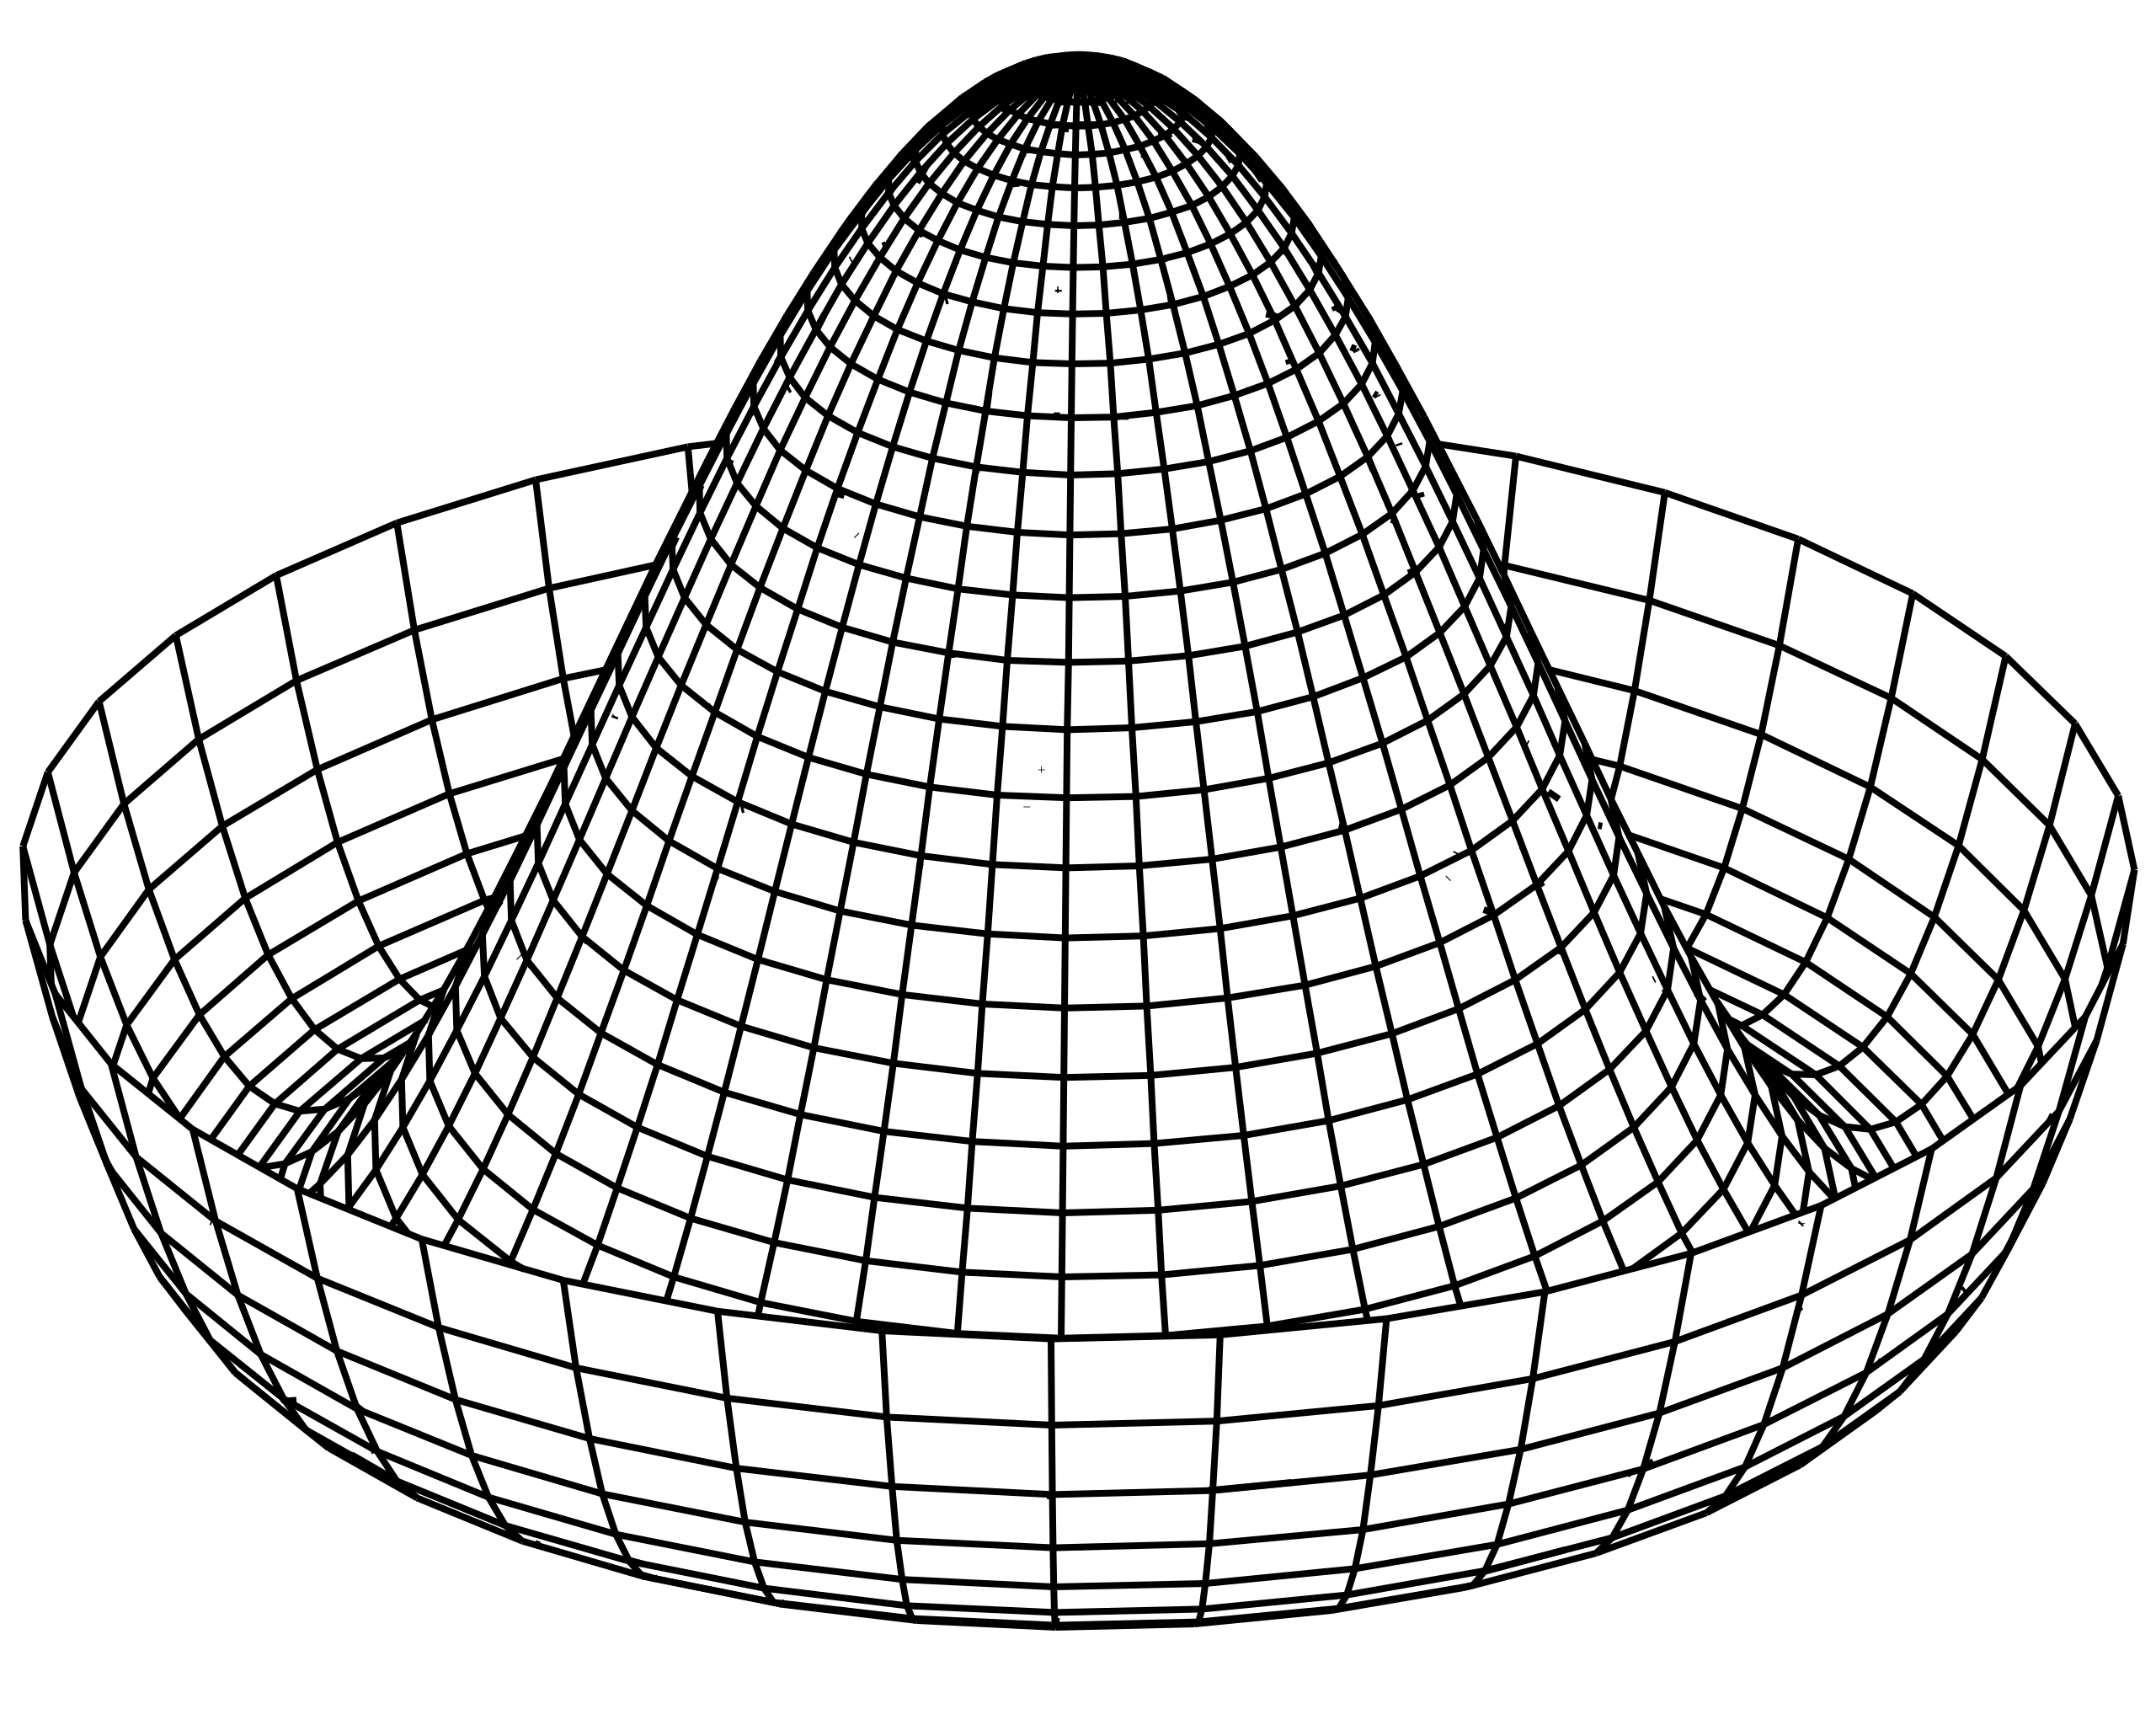
\includegraphics[width=0.5\textwidth]{figures/mexican_hat.png}
\caption{Visualization of $V(\phi)$ as the so-called ``Mexican hat'' potential.}
\label{fig:mexican_hat}
\end{figure}


Undertaking a unitary gauge transformation in SU(2), $\phi^+$ vanishes and $\phi^0$ remains as a physical scalar field.
Expanding this scalar field around the minimum of the potential in Equation~\ref{eq:higgsV}, $\phi^0 \rightarrow \frac{v+H(x)}{\sqrt{2}}$,
where $H(x)$ is a scalar at spacetime position $x$ with expected value 0.

Symmetry breaking alters the terms $\mathcal{L}_\mathrm{\phi}$ and $\mathcal{L}_\mathrm{Yukawa}$ in Equation~\ref{eq:EWpreSSB}, leaving the others unchanged. In a Lagrangian density, the kinetic and potential terms for such a scalar field $\phi$ are
\begin{equation}
\mathcal{L}_\phi = (D_\mu\phi)^\dagger(D^\mu\phi) - V(\phi) \label{eq:Lphi}
\end{equation}
Let us expand Equation~\ref{eq:Lphi} for the $\phi$-field using the previously defined $D_\mu$:
\begin{equation}
\begin{split}
%\mathcal{L}_\mathrm{Yukawa}  & = \sum_f -G_f \bar{f} f (v+H) \\
\mathcal{L}_\mathrm{\phi} & = \frac{1}{2} (\partial^\mu H) (\partial_\mu H) - \lambda\left[ v^2H^2 + vH^3 + \frac{1}{4}H^4\right] \\
& + \frac{1}{8} \left| g \hat{T}^1 A^1_\mu + g \hat{T}^2 A^2_\mu + g \hat{T}^3 A^3_\mu + g' Y B_\mu \right|^2 (v+H)^2
\end{split}
\end{equation}
Noting that $(\hat{T}^1 \pm i \hat{T}^2)/2 \equiv \hat{T}^\pm$ are the raising and lowering operators 
for the third component of weak isospin in the SU(2) symmetry,
and the charge operator $\hat{Q} = \hat{T}^3 - \hat{Y}$,
the last term in $\mathcal{L}_\mathrm{\phi}$ simplifies:
\begin{equation}
\mathcal{L}_\mathrm{\phi} = ... + \frac{1}{8}\left[ g^2(A^1_\mu)^2 + g^2(A^2_\mu)^2  + \left( gA^3_\mu + g' B_\mu \right)^2 \right] (v+H)^2
\end{equation}
If we define a weak angle $\theta_W = \mathrm{arctan}\frac{g'}{g}$, 
we view $gA^3_\mu + g' B_\mu$ as the $A^3$ and B bosons being rotated into two other bosons. 
These will be the massive Z boson and the massless $\gamma$ boson, also known as the photon \cite{Weinberg1967}.
Meanwhile, we can view the $A^1$ and $A^2$ bosons combining to give the charged $W^\pm$ bosons:
\begin{equation}
W^\pm = \frac{A^1 \mp iA^2}{\sqrt{2}} \label{eq:WpmA12}
\end{equation}
For completeness, let us rewrite the electroweak gauge covariant derivative in terms of the physical bosons.
The Z boson is represented by the gauge field $Z_\mu$ and the photon is represented by the gauge field $A_\mu$ without a superscript.
\begin{equation}
\label{eq:covariant_derivative}
D_\mu^\mathrm{EW} = \partial_\mu - \frac{ig}{\sqrt{2}} (W_\mu^+ \hat{T}^+ + W_\mu^- \hat{T}^-) - \frac{ig}{\mathrm{cos}\:\theta_W} Z_\mu( \hat{T}^3 - \mathrm{sin}^2 \: \theta_W \: \hat{Q}) - ie A_\mu \hat{Q}
\end{equation}
We can now rewrite $\mathcal{L}_\mathrm{\phi}$ from before, in terms of the physical W and Z bosons:
\begin{equation}
\label{eq:LhiggsWZ}
\begin{split}
\mathcal{L}_\mathrm{\phi} & = \frac{1}{2} (\partial^\mu H) (\partial_\mu H) - \lambda\left[ v^2H^2 + vH^3 + \frac{1}{4}H^4\right] \\
& + \left[ \frac{g^2}{4} W^+_\mu W^{{-}\mu}  + \frac{g^2}{8\:\mathrm{cos}^2\:\theta_W} Z_\mu Z^\mu \right](v+H)^2   \\
\end{split}
\end{equation}
From this expression, we can extract expressions for the W and Z bosons' masses at leading-order:
\begin{equation}
\label{eq:WZmass}
m_W = \frac{v g}{2},\:\:\:\:m_Z = \frac{vg}{2\:\mathrm{cos}\:\theta_W}
\end{equation}
Lastly, let us we reframe Equation~\ref{eq:EWpreSSB} in terms of the physical gauge bosons.
The antisymmetric photon, Z, and W field strength tensors $A_{\mu\nu}$, $Z_{\mu\nu}$, $W^{\pm}_{\mu\nu}$ are provided as
\begin{equation}
\begin{split}
A_{\mu\nu} &= \partial_\mu A_\nu - \partial_\nu A_\mu \\
Z_{\mu\nu} &= \partial_\mu Z_\nu - \partial_\nu Z_\mu \\
(\vec{\mathbf{W}}^{+}_{\mu\nu})_a &= \partial_\mu (\vec{\mathbf{W}}^{+}_\nu)_a - \partial_\nu (\vec{\mathbf{W}}^{+}_\mu)_a - ig\varepsilon_{abc}(\vec{\mathbf{W}}^{+}_\mu)_b (\vec{\mathbf{W}}^{+}_\nu)_c \\
\vec{\mathbf{W}}^{-}_{\mu\nu} &= (\vec{\mathbf{W}}^{+}_{\mu\nu})^\dagger
\end{split}
\end{equation}
where the vector notation indicates components in three-dimensional weak isospin space.
Einstein summation convention is used and $\varepsilon$ is the antisymmetric Levi-Civita symbol.

Finally, we can write down the full EW Lagrangian density after symmetry breaking. 
As before, $\mathcal{L}_\mathrm{EW} = \mathcal{L}_\mathrm{Gauge} + \mathcal{L}_\mathrm{Fermion} + \mathcal{L}_\mathrm{\phi} + \mathcal{L}_\mathrm{Yukawa}$. 
The $\mathcal{L}_\mathrm{Gauge}$ term contains the gauge field tensor dynamic terms, the triple-gauge couplings, and the quartic-gauge couplings:
\begin{equation} 
\begin{split}
\label{eq:L_Gauge}
\mathcal{L}_\mathrm{Gauge} & = -\frac{1}{4} \termLB A^{\mu\nu} A_{\mu\nu} + 2  W^+_{\mu\nu} W^{{-}\mu\nu} + Z_{\mu\nu} Z^{\mu\nu} \termRB  \\ 
 & - ig \termLB (W^+_{\mu\nu} W^{{-}\mu} - W^{+\mu} W^{{-}}_{\mu\nu})(A^\nu\mathrm{sin}\:\theta_W - Z^\nu \mathrm{cos}\:\theta_W)  \\
 & \qquad\qquad\qquad\qquad\qquad\qquad + W^{{-}}_{\nu} W^+_{\mu} (A^{\mu\nu} \mathrm{sin}\:\theta_W - Z^{\mu\nu} \mathrm{cos} \theta_W ) \termRB  \\
 & + \frac{g^2}{4} \termLB {-}\big( 2 W^+_\mu W^{{-}\mu} + (A_\mu \mathrm{sin}\:\theta_W - Z_\mu \mathrm{cos}\:\theta_W)^2 \big)^2 \\
 & \:\: + \big( W_\mu^+ W_\nu^{{-}} + W_\nu^+ W_\mu^{{-}} + (A_\mu \mathrm{sin}\:\theta_W - Z_\mu \mathrm{cos}\:\theta_W)(A_\nu\mathrm{sin}\:\theta_W - Z_\nu \mathrm{cos}\:\theta_W)\big)^2 \termRB
\end{split}
\end{equation}
The allowed gauge self-coupling vertices are pictured in Figures~\ref{fig:3GC} and~\ref{fig:4GC}.

The $\mathcal{L}_\mathrm{Fermion}$ term contains the interaction between the gauge bosons and the fermions, in the neutral current and the charged current:
\begin{equation}
\begin{split}
\label{eq:L_Fermion}
\mathcal{L}_\mathrm{Fermion} & = \termLB \frac{g}{\mathrm{cos}\:\theta_W} \big(J_\mu^\mathrm{3} - \mathrm{sin}^2\:\theta_W J_\mu^\mathrm{EM} \big) Z^\mu + eJ_\mu^\mathrm{EM} A^\mu \termRB \\
& - \frac{g}{\sqrt{2}} \termLB \big( \bar{u}_i \gamma^\mu \frac{1-\gamma^5}{2} V_{ij} d_j + \bar{\nu}_i \gamma^\mu \frac{1-\gamma^5}{2} e_i \big) W_\mu^+ + \mathrm{h.c.} \termRB
\end{split}
\end{equation}

The electromagnetic current is defined as $J^\mathrm{EM}_\mu \equiv \sum_f q_f \bar{f} \gamma_\mu f$ , with the bilinear covariant $\gamma_\mu$ representing the vector spin-1 coupling.
The weak neutral current is defined as $J^\mathrm{3}_\mu \equiv \sum_f T^3_f \bar{f} \gamma_\mu \frac{1-\gamma^5}{2} f$,
with the bilinear covariant representing the infamous ``vector minus axial'' spin-1 coupling.
The matrix $V_{ij}$ is the CKM matrix.

%This model is renormalizable

%\mathcal{L}_\mathrm{Fermion} & = \termLB \big( e A^\mu \sum_f q_f \bar{f} \gamma_\mu f \big) + \big( \frac{gZ^\mu}{\mathrm{cos}\:\theta_W}( \big)\termRB
%\mathcal{L}_\mathrm{Fermion} & = \sum_{f} \bar{f} i \gamma^\mu \partial_\mu - m_f) f \nonumber \\ 
%\mathcal{L}_\mathrm{\phi}    & = |D_\mu \phi|^2 - \lambda \left( |\phi|^2 - \frac{1}{2} v^2 \right)^2 \nonumber \\
%\mathcal{L}_\mathrm{Yukawa}  & = {-} \sum_f \frac{gm_f}{2m_W} \bar{f} f H \nonumber
%\end{align}
\begin{figure}[!hbt] % 3GC
 \centering
 \begin{tikzpicture} % WWZ
  \begin{feynman}
   \vertex (a2) {\(\boldsymbol{\W^\pm}\)};
   \vertex [right= 1.5cm of a2] (b1);
   \vertex [right= 1.1cm of b1] (c1);
   \vertex [above= 0.9cm of c1] (c2) {\(\boldsymbol{\Z}\)};
   \vertex [below= 0.9cm of c1] (c3) {\(\boldsymbol{\W^\pm}\)};
   
   \diagram* {
    (a2) -- [boson, very thick] (b1),
    (b1) -- [boson, very thick] (c2),
    (b1) -- [boson, very thick] (c3),
   };
  \end{feynman}
 \end{tikzpicture} \hspace{0.5cm}
 \begin{tikzpicture} % WWy
  \begin{feynman}
   \vertex (a2) {\(\boldsymbol{\W^\pm}\)};
   \vertex [right= 1.5cm of a2] (b1);
   \vertex [right= 1.1cm of b1] (c1);
   \vertex [above= 0.9cm of c1] (c2) {\(\boldsymbol{\gamma}\)};
   \vertex [below= 0.9cm of c1] (c3) {\(\boldsymbol{\W^\pm}\)};
   
   \diagram* {
    (a2) -- [boson, very thick] (b1),
    (b1) -- [boson, very thick] (c2),
    (b1) -- [boson, very thick] (c3),
   };
  \end{feynman}
 \end{tikzpicture} 
 \caption{Triple gauge boson vertices in the electroweak theory.} \label{fig:3GC}
\end{figure}

\begin{figure}[!hbt] % 4GC
 \centering
 \begin{tikzpicture} % WWWW
  \begin{feynman}
   \vertex (a1);
   \vertex [above= 0.8cm of a1] (a2) {\(\boldsymbol{\W}\)};
   \vertex [below= 0.8cm of a1] (a3) {\(\boldsymbol{\W}\)};
   \vertex [right= 1.2cm of a1] (b1);
   \vertex [right= 1.2cm of b1] (c1);
   \vertex [above= 0.8cm of c1] (c2) {\(\boldsymbol{\W}\)};
   \vertex [below= 0.8cm of c1] (c3) {\(\boldsymbol{\W}\)};
   
   \diagram* {
    (a2) -- [boson, very thick] (b1),
    (a3) -- [boson, very thick] (b1),
    (b1) -- [boson, very thick] (c2),
    (b1) -- [boson, very thick] (c3),
   };
  \end{feynman}
 \end{tikzpicture} \hspace{0.5cm}
 \begin{tikzpicture} % WWyy
  \begin{feynman}
   \vertex (a1);
   \vertex [above= 0.8cm of a1] (a2) {\(\boldsymbol{\W}\)};
   \vertex [below= 0.8cm of a1] (a3) {\(\boldsymbol{\W}\)};
   \vertex [right= 1.2cm of a1] (b1);
   \vertex [right= 1.2cm of b1] (c1);
   \vertex [above= 0.8cm of c1] (c2) {\(\boldsymbol{\gamma}\)};
   \vertex [below= 0.8cm of c1] (c3) {\(\boldsymbol{\gamma}\)};
   
   \diagram* {
    (a2) -- [boson, very thick] (b1),
    (a3) -- [boson, very thick] (b1),
    (b1) -- [boson, very thick] (c2),
    (b1) -- [boson, very thick] (c3),
   };
  \end{feynman}
 \end{tikzpicture} \hspace{0.5cm}
 \begin{tikzpicture} % WWyZ
  \begin{feynman}
   \vertex (a1);
   \vertex [above= 0.8cm of a1] (a2) {\(\boldsymbol{\W}\)};
   \vertex [below= 0.8cm of a1] (a3) {\(\boldsymbol{\W}\)};
   \vertex [right= 1.2cm of a1] (b1);
   \vertex [right= 1.2cm of b1] (c1);
   \vertex [above= 0.8cm of c1] (c2) {\(\boldsymbol{\gamma}\)};
   \vertex [below= 0.8cm of c1] (c3) {\(\boldsymbol{\Z}\)};
   
   \diagram* {
    (a2) -- [boson, very thick] (b1),
    (a3) -- [boson, very thick] (b1),
    (b1) -- [boson, very thick] (c2),
    (b1) -- [boson, very thick] (c3),
   };
  \end{feynman}
 \end{tikzpicture} \hspace{0.5cm}
 \begin{tikzpicture} % WWZZ
  \begin{feynman}
   \vertex (a1);
   \vertex [above= 0.8cm of a1] (a2) {\(\boldsymbol{\W}\)};
   \vertex [below= 0.8cm of a1] (a3) {\(\boldsymbol{\W}\)};
   \vertex [right= 1.2cm of a1] (b1);
   \vertex [right= 1.2cm of b1] (c1);
   \vertex [above= 0.8cm of c1] (c2) {\(\boldsymbol{\Z}\)};
   \vertex [below= 0.8cm of c1] (c3) {\(\boldsymbol{\Z}\)};
   
   \diagram* {
    (a2) -- [boson, very thick] (b1),
    (a3) -- [boson, very thick] (b1),
    (b1) -- [boson, very thick] (c2),
    (b1) -- [boson, very thick] (c3),
   };
  \end{feynman}
 \end{tikzpicture}
 \caption{Non-Abelian quartic gauge couplings in the electroweak theory.} \label{fig:4GC}
\end{figure}

\subsection{The Higgs boson}

Let us look at the second term of Equation~\ref{eq:LhiggsWZ}.
The portion $-\lambda v^2 H^2 $ suggests to us we can identify the quantum of the $H$-field as a physical boson with mass $m_H = \sqrt{2v^2\lambda}$.
We will call this quantum the Higgs boson, and the field, the Higgs field.

The $\mathcal{L}_\mathrm{\phi}$ term from the electroweak Lagrangian density can be expanded to find the Higgs couplings to itself and the other gauge bosons, in particular to the Z boson which is relevant to this work:

\begin{equation}
\begin{split}
\label{eq:L_phi}
\mathcal{L}_\mathrm{\phi} & = \termLB \frac{1}{2} (\partial^\mu H) (\partial_\mu H) - \frac{1}{2}m_H^2 H^2 \termRB - \termLB \frac{gm_H^2}{4m_W} H^3 + \frac{g^2m_H^2}{32m_W^2}H^4 \termRB \\
& + \termLB \left( W_\mu^+ W^{{-}\mu} + \frac{1}{2\mathrm{cos}^2\:\theta_W} Z_\mu Z^\mu \right) \left( gm_WH+\frac{g^2}{4}H^2 \right) \termRB
\end{split}
\end{equation}

Meanwhile, the $\mathcal{L}_\mathrm{Yukawa}$ term from the Lagrangian density becomes
\begin{equation}
\label{L_Yukawa}
\mathcal{L}_\mathrm{Yukawa} = {-} \sum_f \frac{gm_f}{2m_W} \bar{f}fH
\end{equation}
It provides for the Higgs boson to interact with and decay into fermions,
more likely for massive fermions.
The fermion mass $m_f$ truly arises from the coupling to the Higgs field, and not vice versa.

\begin{figure}[!hbt] % Higgs couplings
 \centering
\begin{tikzpicture} % VVH
  \begin{feynman}
   \vertex (a2) {\(\boldsymbol{\mathrm{V}}\)};
   \vertex [right= 1.3cm of a2] (b1);
   \vertex [right= 1.1cm of b1] (c1);
   \vertex [above= 0.9cm of c1] (c2) {\(\boldsymbol{\Hi}\)};
   \vertex [below= 0.9cm of c1] (c3) {\(\boldsymbol{\mathrm{V}}\)};
   
   \diagram* {
    (a2) -- [boson, very thick] (b1),
    (b1) -- [scalar, very thick] (c2),
    (b1) -- [boson, very thick] (c3),
   };
  \end{feynman}
 \end{tikzpicture} \hspace{0.5cm}
 \begin{tikzpicture} % Hff
  \begin{feynman}
   \vertex (a2) {\(\boldsymbol{f}\)};
   \vertex [right= 1.3cm of a2] (b1);
   \vertex [right= 1.1cm of b1] (c1);
   \vertex [above= 0.9cm of c1] (c2) {\(\boldsymbol{\Hi}\)};
   \vertex [below= 0.9cm of c1] (c3) {\(\boldsymbol{f}\)};
   
   \diagram* {
    (a2) -- [fermion, very thick] (b1),
    (b1) -- [scalar, very thick] (c2),
    (b1) -- [fermion, very thick] (c3),
   };
  \end{feynman}
 \end{tikzpicture} \hspace{0.5cm}
 \begin{tikzpicture} % HHH
  \begin{feynman}
   \vertex (a2) {\(\boldsymbol{\Hi}\)};
   \vertex [right= 1.3cm of a2] (b1);
   \vertex [right= 1.1cm of b1] (c1);
   \vertex [above= 0.9cm of c1] (c2) {\(\boldsymbol{\Hi}\)};
   \vertex [below= 0.9cm of c1] (c3) {\(\boldsymbol{\Hi}\)};
   
   \diagram* {
    (a2) -- [scalar, very thick] (b1),
    (b1) -- [scalar, very thick] (c2),
    (b1) -- [scalar, very thick] (c3),
   };
  \end{feynman}
 \end{tikzpicture} \hspace{0.5cm}
 \begin{tikzpicture} % HHHH
  \begin{feynman}
   \vertex (a1);
   \vertex [above= 0.8cm of a1] (a2) {\(\boldsymbol{\Hi}\)};
   \vertex [below= 0.8cm of a1] (a3) {\(\boldsymbol{\Hi}\)};
   \vertex [right= 1.2cm of a1] (b1);
   \vertex [right= 1.2cm of b1] (c1);
   \vertex [above= 0.8cm of c1] (c2) {\(\boldsymbol{\Hi}\)};
   \vertex [below= 0.8cm of c1] (c3) {\(\boldsymbol{\Hi}\)};
   
   \diagram* {
    (a2) -- [scalar, very thick] (b1),
    (a3) -- [scalar, very thick] (b1),
    (b1) -- [scalar, very thick] (c2),
    (b1) -- [scalar, very thick] (c3),
   };
  \end{feynman}
 \end{tikzpicture}
 \caption{Higgs boson couplings. V is a $\W^\pm$ or $\Z$ boson. $f$ are fermions.}
\end{figure}


\subsection{Strong nuclear force}

The strong nuclear force arises from the theory of the interactions of the quarks and the gluon, called quantum chromodynamics (QCD).
It is a non-Abelian gauge theory whose internal symmetry is represented by the group $\mathrm{SU}(3)$.

Quarks and gluons carry color charge, of which there are three kinds: red, green, and blue.
Negative color charge, carried by the antiquarks and the gluons, is usually represented by the prefix \textit{anti-}, e.g. anti-red.
In transmitting the strong force as its carrier, the gluon carries a positive color charge and a negative color charge.
A gluon could carry red and anti-blue color charge, for example.
There are eight such possible combinations, each of which is a different kind of gluon.
These eight gluons correspond to the eight generators of the $\mathrm{SU}(3)$ group.

Quarks are fermions, having intrinsic spin of 1/2. There are six quarks.
Each quark has a bare mass and an electric charge.
In bound states such as the proton, the quarks appear to weigh more.
This constituent quark mass is heavier because of the field of virtual quarks and gluons around the bare quarks.

\begin{table}[ht]
  \caption{The quarks. When significant, bare masses quote statistical followed by systematic uncertainty. \label{tab:quarks}}
  \begin{center} {\scriptsize
  \begin{tabular}{|p{1.5cm}|c|c|c|c|c|}
  \hline
  \bf{Quark} & \bf{Symbol} & \bf{Charge} & \bf{Isospin} & \bf{Bare mass} $\mathbf{[\MeV\:c^{-2}]}$ & \bf{Constituent mass} $\mathbf{[\MeV\:c^{-2}]}$ \\
  \hline
  Up         & $u$         & {+2/3}      & +1/2         & $2.3 \pm 0.7 \pm 0.5    $  & 336                               \\
  Down       & $d$         & {-1/3}      & -1/2         & $4.8 \pm 0.5 \pm 0.3    $  & 340                               \\
  Charm      & $c$         & {+2/3}      & 0            & $1275 \pm 25            $  & 1550                              \\
  Strange    & $s$         & {-2/3}      & 0            & $95 \pm 5               $  & 486                               \\
  Top        & $t$         & {+2/3}      & 0            & $173,210 \pm 510 \pm 710$  & 4730                              \\
  Bottom     & $b$         & {-1/3}      & 0            & $4180 \pm 30            $  & 177,000                           \\
  \hline
  \end{tabular}
  }
  \end{center}
\end{table}

The Dirac Lagrangian density which defines the interactions between quarks and gluons is
\begin{equation}
\mathcal{L}_\mathrm{QCD} = \sum_{\psi} \bar{\psi}_i \left( i \gamma^\mu ( \partial_\mu \delta_{ij} - i g_s G^a_\mu T^a_{ij}) - m_\psi \delta_{ij} \right) \psi_j - \frac{1}{4} G^a_{\mu\nu} G^{\mu\nu}_a
\end{equation}


\begin{itemize}
  \setlength\itemsep{0em}
  \item The index $a$ represents the eight gluons.
  \item The index $i$ represents the three colors.
  \item The indices $\mu,\nu$ represent spacetime.
  \item $g_s$ is the strong coupling constant, sometimes expressed as $\sqrt{4\pi\alpha_s}$ which varies as a function of energy scale (see Figure~\ref{fig:alphaS}.
  \item $\psi_i$ is a Dirac bi-spinor representing the field for a quark and its antiquark at spacetime point $x$. $\bar{\psi}_i$ is the adjoint as in section~\ref{qed}.
  \item $G^a_\mu$ is the $\mathrm{SU}(3)$ gauge field.
  \item $T^a_{ij}$ are the eight generators of the $\mathrm{SU}(3)$ group, also known as Gell-Mann matrices.
  \item Lastly, the symbol $G^a_{\mu\nu}$ is the gluon field strength tensor...
\end{itemize}
The gluon field strength tensor comes from the gluon fields, $\mathcal{A}^a_\mu(x)$, as such:
\begin{equation}
G^a_{\mu\nu} = \partial_\mu \mathcal{A}^a_\nu - \partial_\nu \mathcal{A}^a_\mu + g\:f^{abc} \mathcal{A}^b_\mu \mathcal{A}^c_\nu
\end{equation}
This quantum field theory permits the quark-quark-gluon vertex, the three-gluon vertex, and the four-gluon vertex.
\begin{figure}[!hbtp]
  \centering
    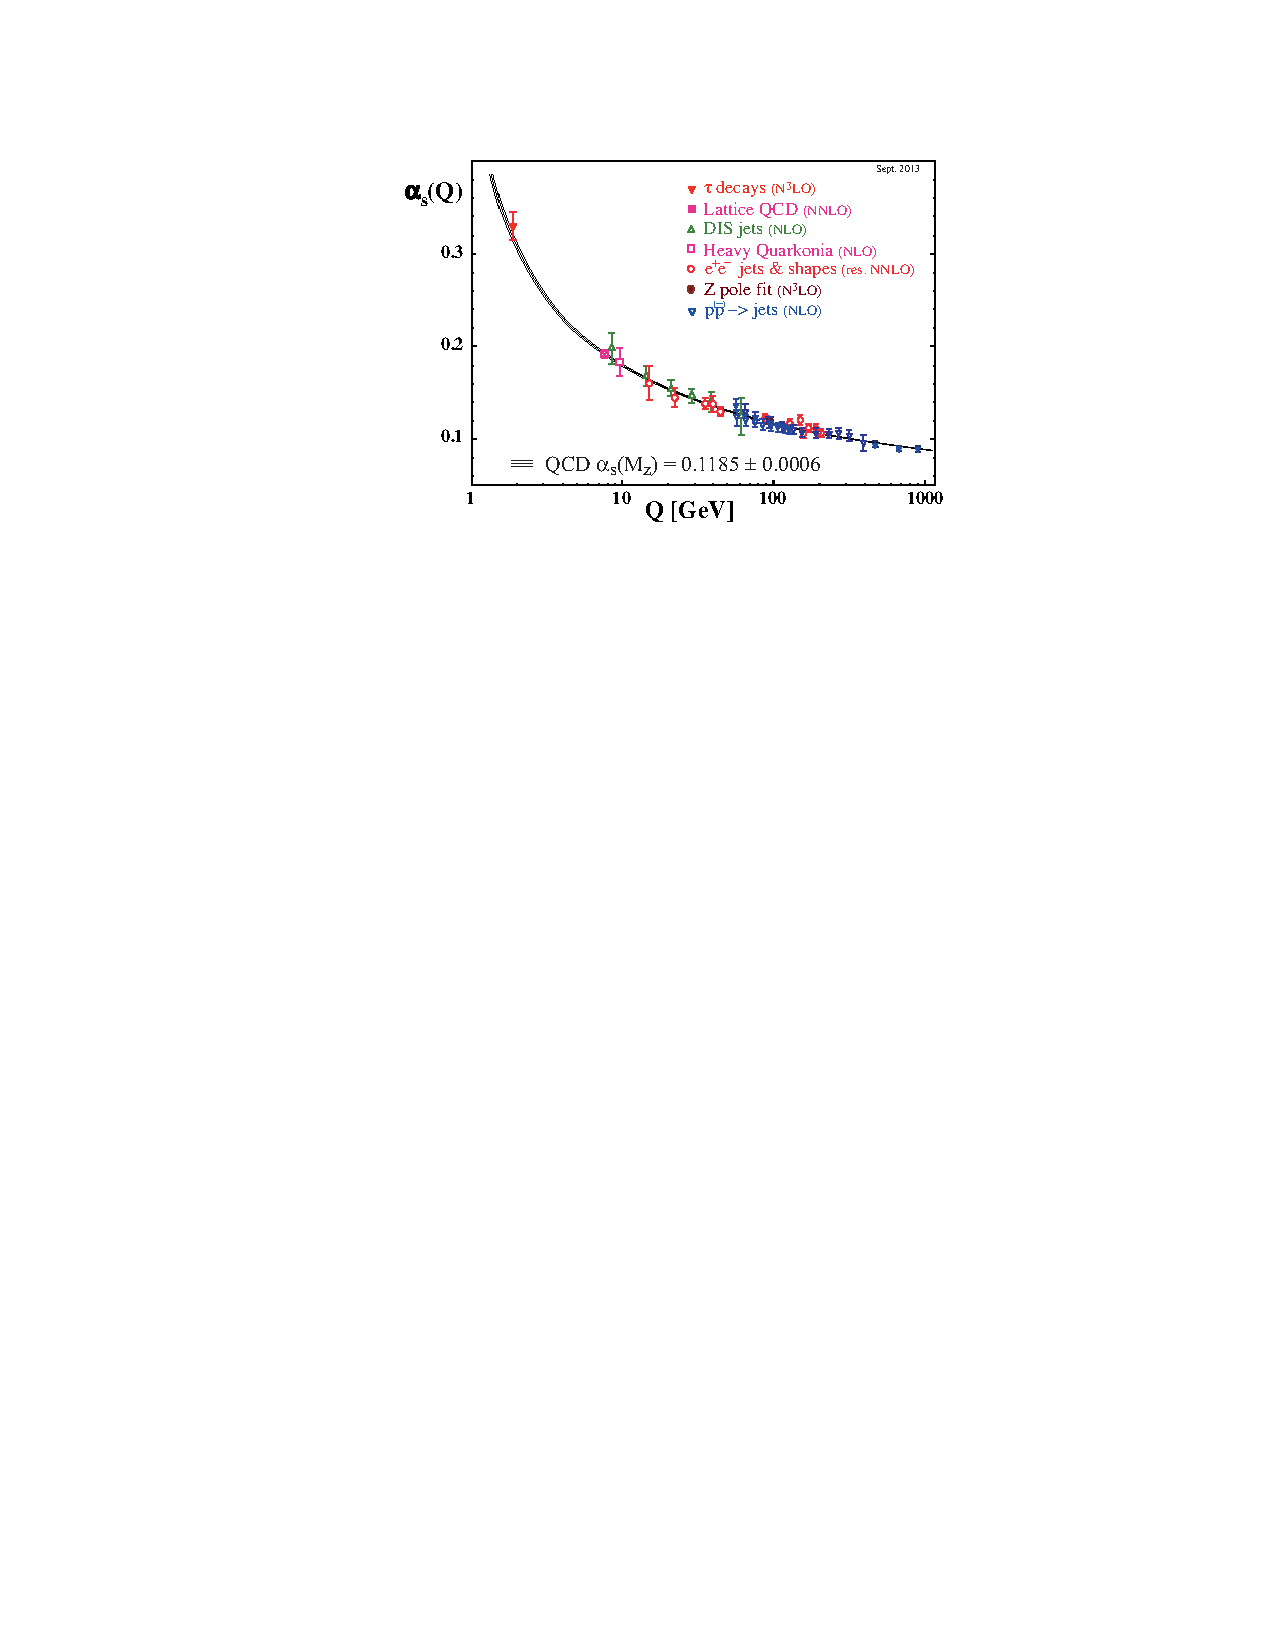
\includegraphics[width=0.80\textwidth]{figures/alphaS_running.pdf}
  \caption{The so-called ``running'' of $\alpha_S$ as the energy scale ~\cite{PhysRevD.98.030001}.} 
  \label{fig:alphaS}
\end{figure}

% Diagram
For experimental physics at the LHC, QCD is important even for studying electroweak processes.
Since we collide protons, the internal dynamics of the proton are an essential ingredient of Monte Carlo simulations.
The momentum fractions carried by the quarks and gluons are determined empirically as what are called the proton parton distribution functions.
Internal gluon loop corrections and the possibility of emitting extra gluons before or after the hard process can enhance the total cross section significantly for physics processes.
QCD activity resulting in charged hadrons may interfere with the ability to identify charged leptons in physics events of interest.
%Lastly, the hadronic radiation from the interaction point irradiates the detector components. This changes their material properties over time.
\clearpage
\section{Proton parton distribution functions}

The quarks and gluons inside a proton are collectively called partons.
The parton distribution functions (PDFs) $f_i(x,Q^2)$ give the probability of finding inside the proton a quark or gluon with momentum fraction $x$, in a hard process with momentum transfer $Q$.
According to the central feature of QCD, known as asymptotic freedom, the partonic interactions become asymptotically weak at short distances.
QCD can quantitatively predict the dependence of the PDFs on the energy scale, $Q^2$,
by way of the QCD evolution equations developed by Dokshitzer, Gribov, Lipatov, Altarelli, and Parisi (DGLAP).
These equations are valid in the regime where the strong coupling constant is small ($\alpha_S(Q^2) \ll 1$) so perturbative calculations are effective.
The DGLAP equations can make a statement about the $Q^2$ dependence, but the $x$ dependence is still unknown.
By the QCD factorization theorems, the PDFs can be related to the observable cross section of a
hard process by writing the cross section as a parton interaction convoluted with the PDFs \cite{Collins:1989gx}.
The parton interaction can be calculated using perturbative quantum field theory techniques.
The PDF shapes as a function of $x$ are not calculated theoretically and are instead determined empirically by experimental data.

\begin{figure}[hb]
  \centering
    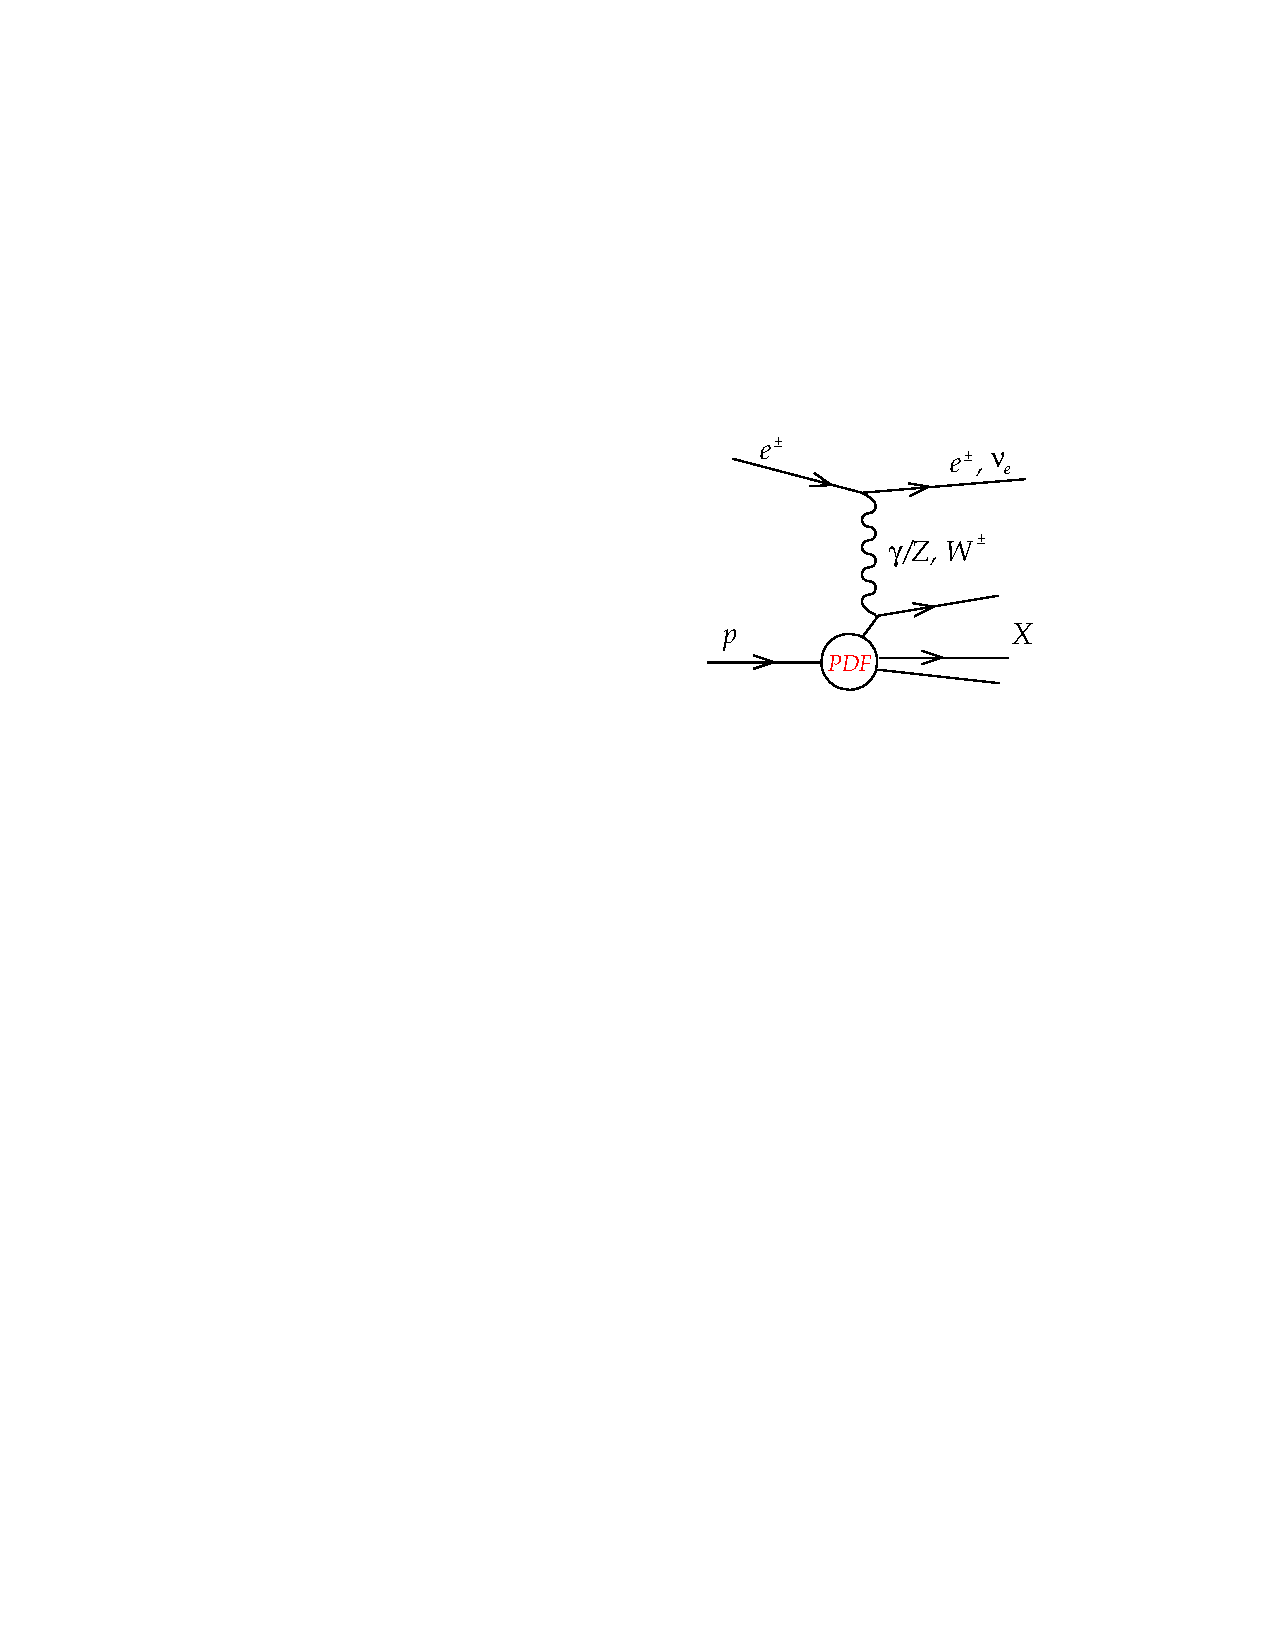
\includegraphics[width=0.50\textwidth]{figures/dis.pdf}
  \caption{Probing the PDFs with deep inelastic scattering. From \cite{Placakyte:2011az}.} 
  \label{fig:dis}
\end{figure}

The HERA experiment provided important data for the PDF determination by performing
deep inelastic scattering of electrons or positrons with protons, 
at center of mass energies of a few hundred \GeV.
Two different scattering processes can occur, called the neutral current and charged current; see Figure~\ref{fig:dis}.
In the charged current interaction, the cross sections of electron and positron on proton are sensitive to different quark PDFs.
%The neutral current $ep$ cross section can be expressed in terms of the structure functions $\tilde{F}$:
%\begin{equation}
%\frac{d^2 \sigma^{e^\pm p}_\mathrm{N.C.}}{dx\:dQ^2} = \frac{2 \pi \alpha^2}{xQ^4}\termLB Y_+ \tilde{F}^\pm_2 \mp Y_{-} x \tilde{F}^\pm_3 - y^2 \tilde{F}^\pm_L \termRB
%\end{equation}
%where $Y_\pm = 1 \pm (1-y^2)$ as a function of the inelasticity $y$.
%In general, $\tilde{F}_2$ dominates, $x\tilde{F^3}$ becomes important at higher $Q^2$,
%and $\tilde{F}_L$ only matters for significant $y$.
%The PDFs are directly related to these structure functions.
%Neglecting higher-order terms for the gluon density: $F_2$ is approximately the momentum sum of the 
%distributions of quarks and antiquarks ($F_2 \approx x\sum e_q^2 (q+\bar{q})$) 
%and $F_3$ is approximately their momentum difference ($xF_3 \approx x\sum 2e_qa_q(q-\bar{q}))$.
%
%The charged current $ep$ cross section can also be expressed in terms of structure functions.

In $p\bar{p}$ and $pp$ collisions at the Tevatron and LHC,
we can learn more about the proton PDFs through Standard Model precision measurements.
In particular, the Z boson differential cross section studied in this work contributes to the global fit of the quark distributions.
Meanwhile, ultraperipheral lead-lead heavy ion collisions are also an unconventional source of high energy photon probes which help us study the gluon distribution down to very small values of $x$ (see~\cite{Baltz:2007kq}).
Overall, the PDFs are an important quantity for simulating the Standard Model background in a search for new physics.
An example of the PDF set provided by the NNPDF collaboration at $Q=50 \GeV$ is shown in Figure~\ref{fig:pdfq50}.

\begin{figure}[hbtp]
  \centering
    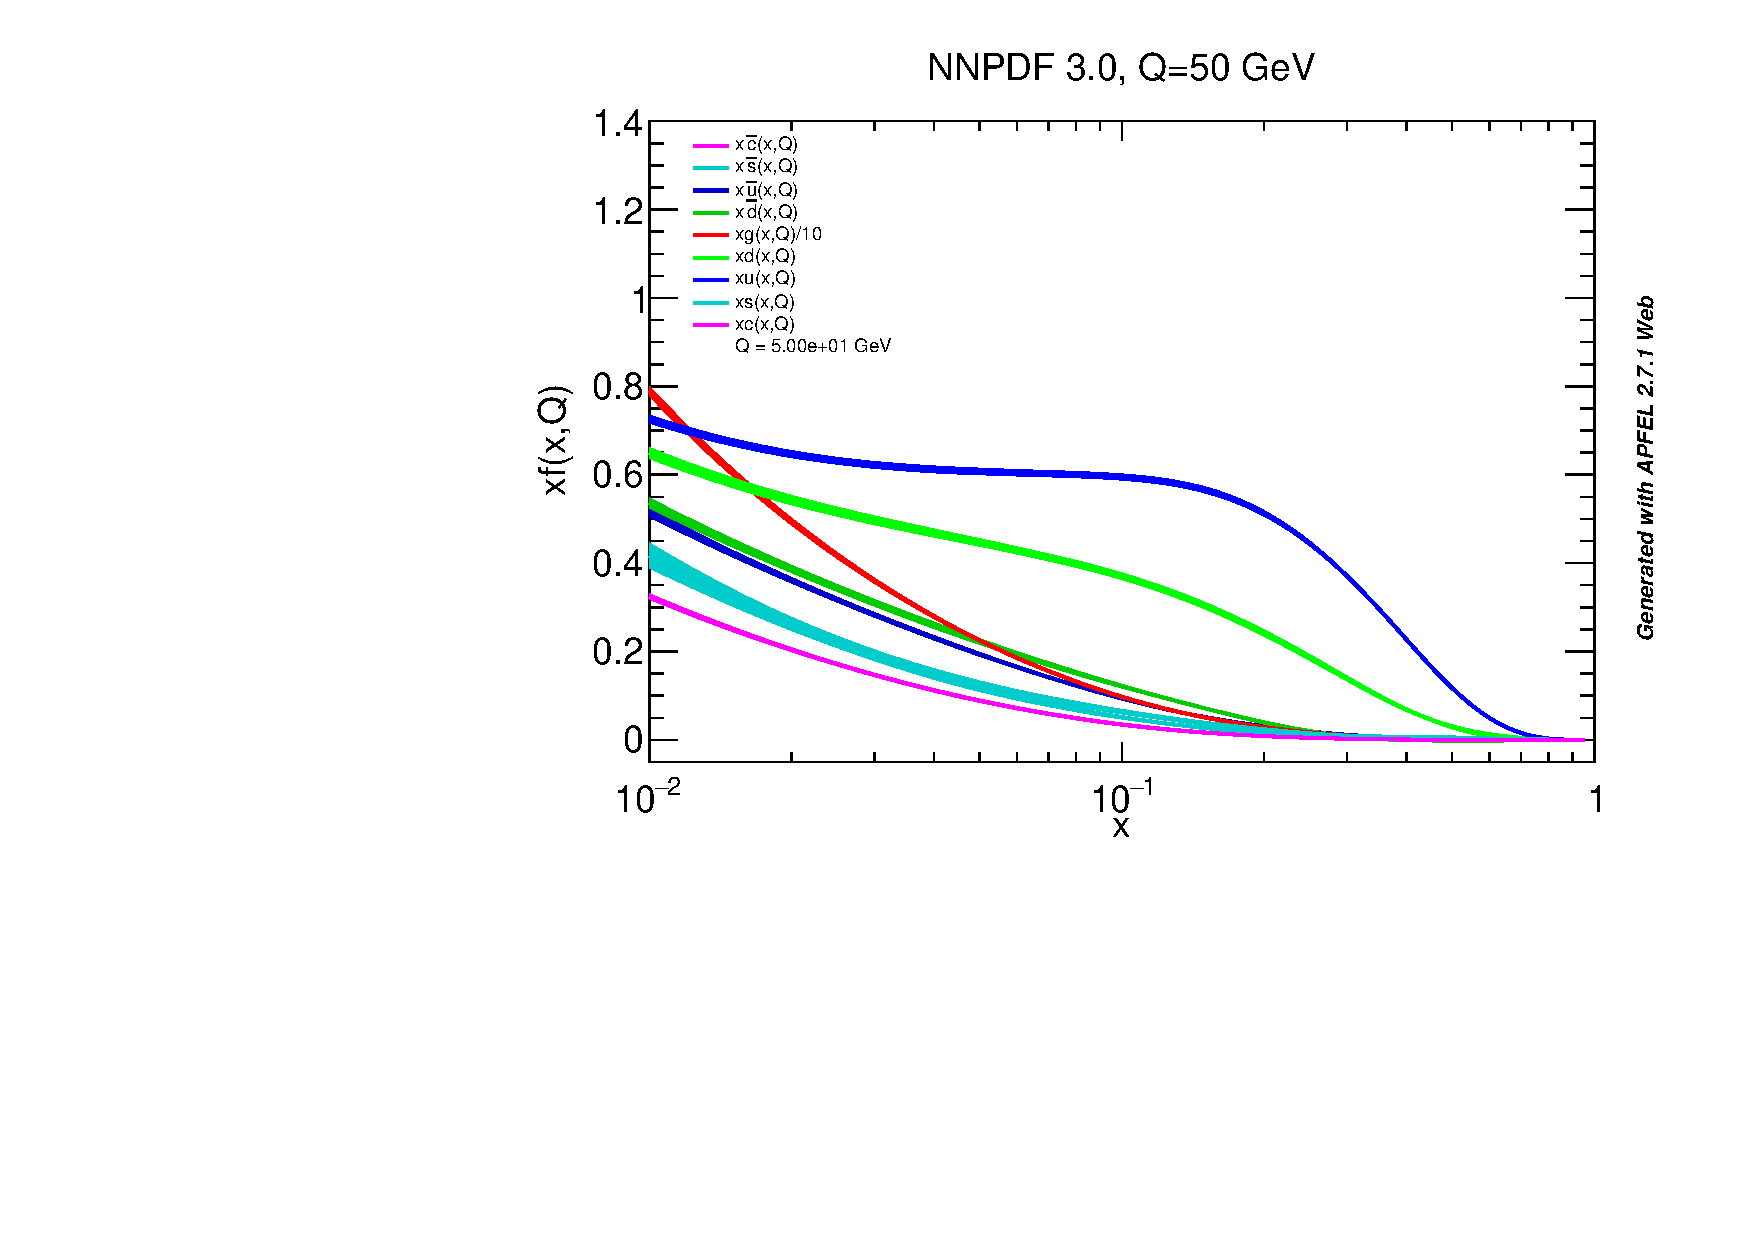
\includegraphics[width=0.90\textwidth]{figures/nnpdf30_115_Q50_v4.pdf}
  \caption{NNPDF 3.0 set at momentum transfer 50 \GeV. Presented in~\cite{nnpdf}.} 
  \label{fig:pdfq50}
\end{figure}

\section{New physics}
\label{sec:bsmtheory}
%In this work, we consider a scenario in which are produced a pair of charged leptons ($\ell^{+}\ell^{-}$, where $\ell=\Pe$ or $\Pgm$),
%consistent with the decay of a $\PZ$ boson, together with large missing transverse momentum ($\met$).

The study presented here considers one possible mechanism for producing weakly interacting massive particles at the LHC~\cite{Abercrombie:2015wmb}.
In this scenario, a $\PZ$ boson, produced in $pp$ collisions, recoils against a pair of DM particles, $\chi\overline\chi$.
The $\PZ$ boson subsequently decays into two charged leptons (electrons or muons), 
%producing a low-background dilepton signature, 
recoiling against $\met$ due to the undetected DM particles. 
We assume the final state dark matter particle $\chi$ is a Dirac fermion.

\begin{figure} % BSM models
 \centering
 \begin{tikzpicture} % ZH(inv)
  \begin{feynman}
   \vertex (q1) {\(\boldsymbol{\Pq}\)};
   \vertex [below= 3cm of q1] (q2) {\(\boldsymbol{\Paq}\)};
   \vertex [right= 1.6cm of q1] (a1);
   \vertex [below= 1.5cm of a1] (a2);
   \vertex [right= 1.6cm of a2] (b1);
   \vertex [right= 1.6cm of b1] (c1);
   \vertex [above= 1.3cm of c1] (c2);
   \vertex [below= 1.3cm of c1] (c3);
   \vertex [right= 1cm of c2] (d1);
   \vertex [right= 1cm of c3] (d2);
   \vertex [above= 0.3cm of d1] (f1) {\(\boldsymbol{\ell}\)};
   \vertex [below= 0.3cm of d1] (f2) {\(\boldsymbol{\bar{\ell}}\)};
   \vertex [above= 0.3cm of d2] (f3) {\(\boldsymbol{\chi}\)};
   \vertex [below= 0.3cm of d2] (f4) {\(\boldsymbol{\bar{\chi}}\)};
   
   \diagram* {
    (q1) -- [fermion, very thick] (a2),
    (q2) -- [anti fermion, very thick] (a2),
    (a2) -- [boson, very thick, edge label'=\(\boldsymbol{\Z^*}\)] (b1),
    (b1) -- [boson, very thick, edge label=\(\boldsymbol{\Z}\)] (c2),
    (b1) -- [scalar, very thick, edge label=\(\boldsymbol{\Hi}\)] (c3),
    (c2) -- [fermion, very thick] (f1),
    (c2) -- [anti fermion, very thick] (f2),
    (c3) -- [fermion, very thick] (f3),
    (c3) -- [anti fermion, very thick] (f4),
   };
  \end{feynman}
 \end{tikzpicture} \hspace{1cm}
 \begin{tikzpicture} % Simplified model spin-0 mediator
  \begin{feynman}
   \vertex (g1) {\(\boldsymbol{}\)};
   \vertex [below= 3.6cm of g1] (g2) {\(\boldsymbol{}\)};
   \vertex [right= 1.4cm of g1] (a1);
   \vertex [right= 1.4cm of g2] (a2);
   \vertex [below= 0.8cm of a1] (a3);
   \vertex [above= 0.8cm of a2] (a4);
   \vertex [right= 1.4cm of a3] (b1);
   \vertex [right= 1.4cm of a4] (b2);
   \vertex [right= 1.4cm of b1] (c1);
   \vertex [right= 1.4cm of b2] (c2);
   \vertex [right= 1cm of c1] (d1);
   \vertex [right= 1cm of c2] (d2);
   \vertex [above= 0.3cm of d1] (f1) {\(\boldsymbol{\ell}\)};
   \vertex [below= 0.3cm of d1] (f2) {\(\boldsymbol{\bar{\ell}}\)};
   \vertex [above= 0.3cm of d2] (f3) {\(\boldsymbol{\chi}\)};
   \vertex [below= 0.3cm of d2] (f4) {\(\boldsymbol{\bar{\chi}}\)};
   \vertex [below = 0.2cm of b2] (dm1) {\(\boldsymbol{g_\Pq}\)};
   \vertex [below = 0.2cm of c2] (dm2) {\(\boldsymbol{g_\mathrm{DM}}\)};
   
   \diagram* {
    (g1) -- [gluon, very thick] (a3),
    (g2) -- [gluon, very thick] (a4),
    (a3) -- [fermion, very thick, edge label'=\(\boldsymbol{\bar{\Top}}\)] (a4) -- [fermion, very thick, edge label=\(\boldsymbol{\Top}\)] (b2) -- [fermion, very thick, edge label=\(\boldsymbol{\bar{\Top}}\)] (b1) -- [fermion, very thick, edge label'=\(\boldsymbol{\Top}\)] (a3),
    (b1) -- [boson, very thick, edge label=\(\boldsymbol{\Z}\)] (c1),
    (b2) -- [scalar, very thick, edge label=\(\boldsymbol{\phi}\)] (c2),
    (c1) -- [fermion, very thick] (f1),
    (c1) -- [anti fermion, very thick] (f2),
    (c2) -- [fermion, very thick] (f3),
    (c2) -- [anti fermion, very thick] (f4),
   };
  \draw[fill=blue,line width=0pt] (b2) circle(1.5mm);
  \draw[fill=violet,line width=0pt] (c2) circle(1.5mm);
  \end{feynman}
 \end{tikzpicture} \vspace{1cm}
 
 \begin{tikzpicture} % Simplified model spin-1 mediator
  \begin{feynman}
   \vertex (q1) {\(\boldsymbol{\Pq}\)};
   \vertex [below= 3.6cm of q1] (q2) {\(\boldsymbol{\Paq}\)};
   \vertex [right= 2cm of q1] (a1);
   \vertex [right= 2cm of q2] (a2);
   \vertex [below= 0.8cm of a1] (a3);
   \vertex [above= 0.8cm of a2] (a4);
   \vertex [right= 2cm of a3] (b1);
   \vertex [right= 2cm of a4] (b2);
   \vertex [right= 1.5cm of b1] (c1);
   \vertex [right= 1.5cm of b2] (c2);
   \vertex [above= 0.3cm of c1] (f1) {\(\boldsymbol{\ell}\)};
   \vertex [below= 0.3cm of c1] (f2) {\(\boldsymbol{\bar{\ell}}\)};
   \vertex [below= 0.2cm of c2] (U) {\(\boldsymbol{\mathcal{U}/\mathcal{G}}\)};
   
   \diagram* {
    (q1) -- [fermion, very thick] (a3),
    (a3) -- [fermion, very thick] (a4),
    (q2) -- [anti fermion, very thick] (a4),
    (a3) -- [boson, very thick, edge label=\(\boldsymbol{\Z}\)] (b1),
    (a4) -- [ghost, very thick] (U),
    (b1) -- [fermion, very thick] (f1),
    (b1) -- [anti fermion, very thick] (f2),
   };
  \draw[fill=black,line width=0pt] (a4) circle(2.2mm);
  \draw[pattern=north east lines, pattern color=white] (a4) circle(2.2mm);
  \end{feynman}
 \end{tikzpicture} \hspace{1cm}  
 \begin{tikzpicture} % ADD/unparticles
  \begin{feynman}
   \vertex (q1) {\(\boldsymbol{\Pq}\)};
   \vertex [below= 3.6cm of q1] (q2) {\(\boldsymbol{\Paq}\)};
   \vertex [right= 2cm of q1] (a1);
   \vertex [right= 2cm of q2] (a2);
   \vertex [below= 0.8cm of a1] (a3);
   \vertex [above= 0.8cm of a2] (a4);
   \vertex [right= 2cm of a3] (b1);
   \vertex [right= 2cm of a4] (b2);
   \vertex [right= 1.5cm of b1] (c1);
   \vertex [right= 1.5cm of b2] (c2);
   \vertex [above= 0.3cm of c1] (f1) {\(\boldsymbol{\ell}\)};
   \vertex [below= 0.3cm of c1] (f2) {\(\boldsymbol{\bar{\ell}}\)};
   \vertex [above= 0.3cm of c2] (f3) {\(\boldsymbol{\chi}\)};
   \vertex [below= 0.3cm of c2] (f4) {\(\boldsymbol{\bar{\chi}}\)};
   \vertex [below = 0.2cm of a4] (dm1) {\(\boldsymbol{g_\Pq}\)};
   \vertex [below = 0.2cm of b2] (dm2) {\(\boldsymbol{g_\mathrm{DM}}\)};
   
   \diagram* {
    (q1) -- [fermion, very thick] (a3),
    (a3) -- [fermion, very thick] (a4),
    (q2) -- [anti fermion, very thick] (a4),
    (a3) -- [boson, very thick, edge label=\(\boldsymbol{\Z}\)] (b1),
    (a4) -- [boson, very thick, edge label=\(\boldsymbol{\mathcal{A}}\)] (b2),
    (b1) -- [fermion, very thick] (f1),
    (b1) -- [anti fermion, very thick] (f2),
    (b2) -- [fermion, very thick] (f3),
    (b2) -- [anti fermion, very thick] (f4),
   };
  \draw[fill=blue,line width=0pt] (a4) circle(1.5mm);
  \draw[fill=violet,line width=0pt] (b2) circle(1.5mm);
  \end{feynman}
 \end{tikzpicture}
 \caption{Some diagrams beyond the Standard Model in which are produced two charged leptons and missing energy. Clockwise from upper left: associated production of an invisible Higgs boson; gluon-induced production of a Z boson and a massive spin-0 dark matter mediator via top-quark loop; production of a Z boson and a massive spin-1 dark matter mediator; production of a Z boson in association with gravitons (ADD model) or unparticles.} \label{fig:BSMdiagrams}
\end{figure}

\subsection{Simplified models}
Four simplified models of DM production via an $s$-channel mediator exchange are considered.
In these models, the mediator has a spin of 1 (0) and vector or axial-vector (scalar or pseudoscalar) couplings to quarks and DM particles.
The free parameters of each model are the masses $m_{\rm med}$ and $m_{\rm DM}$ of the mediator and DM particle, respectively, as well as the coupling
constant $g_{\Pq}$ ($g_{\rm DM}$) between the mediator and the quarks (DM particles).
The vector coupling model is described with the following Lagrangian:

\begin{equation*}
\mathcal{L}_{\text{vector}} = g_{\rm DM} {Z'}_{\mu}\overline{\chi}\gamma^{\mu}\chi  + g_{\Pq} \sum_{\Pq} {Z'}_{\mu} \overline{\Pq}\gamma^{\mu}\Pq
\end{equation*}

\noindent where the spin-1 mediator is denoted as $\PZ'$ and the SM quark fields are referred to as \PQq and $\overline{\PQq}$.
The Lagrangian for an axial-vector coupling is obtained by making the replacement $\gamma^\mu\rightarrow\gamma^5\gamma^\mu$.
In the case of a spin-0 mediator $\phi$, the couplings between mediator and quarks are assumed to be Yukawa-like, with $g_{\Pq}$ acting as a 
multiplicative modifier for the SM Yukawa coupling ${y_{\Pq} = \sqrt{2}m_{\Pq}/v}$ (where $v = 246 \GeV$ is the SM Higgs field vacuum expectation value),
leading to the Lagrangian:

\begin{equation*}
\mathcal{L}_{\text{scalar}} = g_{\rm DM} {\phi}\overline{\chi}\chi  + g_{\Pq} \frac{\phi}{\sqrt{2}}\sum_{\Pq} y_{\Pq} \overline{\Pq}\Pq.
\end{equation*}

\noindent The Lagrangian with pseudoscalar couplings is obtained by inserting a factor of $i\gamma^5$ into each of the two terms (i.e., $\bar\chi\chi \to i\bar\chi\gamma^5\chi$ and $\bar \Pq \Pq \to i\bar \Pq\gamma^5 \Pq$). Example diagrams of DM production via spin-0 and spin-1 mediators are shown in Fig.~\ref{fig:BSMdiagrams} (upper right and lower right, respectively).

%\begin{figure}[!hbtp]
%  \centering
%    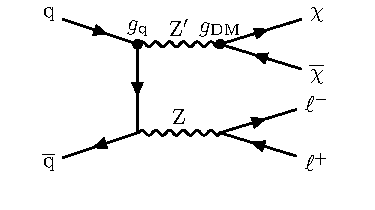
\includegraphics[width=0.45\textwidth]{figures/dmSimpFeynman.pdf}
%    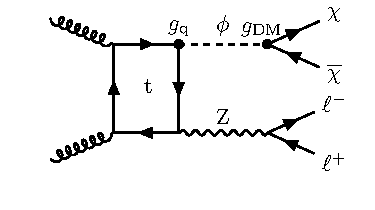
\includegraphics[width=0.45\textwidth]{figures/dmSimpFeynman_spin0.pdf}
%    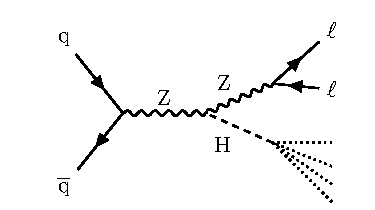
\includegraphics[width=0.45\textwidth]{figures/higgsInvisibleFeynman.pdf}
%    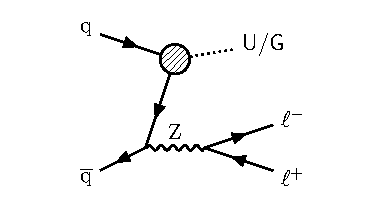
\includegraphics[width=0.45\textwidth]{figures/graph_UG.pdf}
%  \caption{Feynman diagrams illustrative of the processes beyond the SM considered in this paper:
%    (upper left)~DM production in a simplified model with a spin-1 mediator $\PZ'$;
%    (upper right)~DM production in a simplified model with a spin-0 mediator $\phi$;
%    (lower left)~production of a Higgs boson in association with Z boson with subsequent decay of the Higgs boson into invisible particles;
%    (lower right)~unparticle or graviton production. The diagrams were drawn using the {\sc TikZ-Feynman} package~\cite{Ellis:2016jkw}.
%  } 
%      \label{fig:Feynman}
%\end{figure}

\subsection{Invisible Higgs bosons}

A primary focus of the LHC physics program after the discovery of the Higgs boson ~\cite{AtlasPaperCombination,CMSPaperCombination} by
the ATLAS and CMS Collaborations is the study of the properties of this new particle. The observation of a sizable branching
fraction of the Higgs boson to invisible states~\cite{Ghosh:2012ep,Martin:1999qf,Bai:2011wz} would be a strong sign
of BSM physics.  Supersymmetric (SUSY) models embodying R-parity conservation contain a stable neutral lightest SUSY
particle (LSP), e.g., the lightest neutralino~\cite{Belanger:2001am}, leading to the possibility of decays of the Higgs boson into pairs of LSPs.
Certain models with extra spatial dimensions predict graviscalars that could mix with the
Higgs boson~\cite{Giudice:2000av}.  As a consequence, the Higgs boson could oscillate
to a graviscalar and disappear from the SM brane. The signature would be
equivalent to an invisible decay of the Higgs boson. There could also be contributions
from Higgs boson decays into graviscalars~\cite{Battaglia:2004js}.
Other ``Higgs portal'' models~\cite{Baek:2012se,Djouadi:2011aa,Djouadi:2012zc} construct
a generic connection between SM and DM particles via a Higgs boson mediator.
This work considers decays into invisible particles of an SM-like Higgs boson produced in association with a $\PZ$ boson, as shown in Fig.~\ref{fig:BSMdiagrams} (upper left).

\subsection{Extra dimensions}

A popular BSM paradigm considered here is the Arkani-Hamed--Dimopoulos--Dvali (ADD) model with large extra spatial dimensions~\cite{arkani98:hlz,arkani99:hlz,han99:hlz}, which
is motivated by the hierarchy problem, i.e., the disparity between the electroweak unification
scale ($M_\mathrm{EW} \sim 1\TeV$) and the Planck scale ($M_\mathrm{Pl} \sim 10^{16}\TeV$).
The Planck scale is the energy scale at which quantum effects of gravity become dominant and the Standard Model becomes unified with gravitation.
In the ADD model, the apparent Planck scale in four space-time dimensions
is given by $M_\mathrm{Pl}^2 \approx M_\mathrm{D}^{n+2}R^n$, where $M_\mathrm{D}$ is the true Planck scale of
the full $n$+4 dimensional space-time and $R$ is the compactification radius of the extra
dimensions.
The meaning of compactification is that the extra dimensions are finite or periodic in length.
In the limit of sufficiently high length scales or low energy scales, no fields depend on this extra dimension, so it reduces to a standard 4-dimensional space-time.
Assuming $M_\mathrm{D}$ is of the same order as $M_\mathrm{EW}$, the observed large value
of $M_\mathrm{Pl}$ points to an $R$ of order 1 mm to 1 fm for 2 to 7 extra dimensions.
The consequence of the large compactification scale is that the mass spectrum of the
Kaluza--Klein graviton states becomes nearly continuous, resulting in a broad $\PZ$ boson transverse momentum (\PT) spectrum.
Therefore, this model predicts graviton (\cPG) production via the process $\PQq\PAQq \rightarrow \PZ + \cPG$.
The graviton escapes detection, leading to the signature of a Z boson and missing energy (Fig.~\ref{fig:BSMdiagrams}, lower right).

\subsection{Unparticles}

The final BSM model considered in this work is the phenomenologically interesting concept of unparticles, which appear in the low-energy limit of conformal field theories.
In the Standard Model, only massless particles exhibit scale invariance.
Undertaking a scale transformation, all dimensional quantities are multipled by a rescaling factor
raised to the mass dimension. Thus, the massless particle's mass is unaffected.
Unparticles arise from massive BSM fields which scale with fractional dimensions ~\cite{Kang:2014cia,Rinaldi:2014gha,Cheng:1988zx}. 
In other words, the field's quantities are multiplied by fractional powers of the rescaling parameter, allowing for scale invariance.


In the high-energy regime, a scale invariant Banks--Zaks field with a nontrivial infrared fixed point is introduced~\cite{Banks:1981nn}.
The interaction between the SM and Banks--Zaks sectors is mediated by particles of large mass scale $M_{\textsf{U}}$, below which the interaction is suppressed and can be treated
via an effective field theory (EFT). The low-energy regime will include unparticles.
%, which have phase space factors equivalent to those of a noninteger
%number of ordinary particles
In this work, the emission of spin-0 unparticles from SM quarks is considered.
Because of the weakness of the unparticle interactions with the SM fields, the unparticle evades detection.
The EFT Lagrangian used to interpret the results is defined as follows:

\begin{equation*}
\mathcal{L}_{U}  = \frac{\lambda}{\LU^{\dU-1}} \mathcal{O}_{\textsf{U}} \overline{\PQq}\PQq,
\end{equation*}

\noindent where $\lambda$ represents the coupling between the SM and unparticle fields, \LU is the cutoff scale of the EFT, and \dU is the characteristic scaling dimension of the theory.
The unparticle operator is denoted as $\mathcal{O}_{\textsf{U}}$.
A representative Feynman diagram of the interaction is shown in Fig.~\ref{fig:BSMdiagrams} (lower right).



\chapter{Experimental apparatus}

The data studied in this work were collected at the Compact Muon Solenoid (CMS) Experiment.
The CMS detector is a multi-purpose apparatus which records the particle collisions
of the Large Hadron Collider.
It is installed about 100 meters underground close to the French village of Cessy,
between Lake Geneva and the Jura mountains.


\section{The Large Hadron Collider}

The LHC is a two-ring superconducting hadron accelerator \cite{lhcmachine}.
It is designed to collide counter-rotating proton beams with a center-of-mass energy of 14 TeV
and instantaneous luminosity of $10^{34}$ cm\textsuperscript{-2}s\textsuperscript{-1}.
In 2016, protons were collided at at center-of-mass energy of 13 TeV. 
The LHC has also collided lead ions with an energy of 2.8 TeV per nucleon and xenon ions with 2.72 TeV per nucleon.

First, hydrogen atoms are stripped of their protons with a large electric field.
They are accelerated to 450 GeV in the CERN LHC injector chain \cite{lhcinjector}.
The chain is as follows: Linac2 (50 MeV), Proton Synchotron Booster (1.4 GeV), Proton Synchotron (25 GeV), Super Proton Synchotron (450 GeV).
After the SPS, the protons are injected into the LHC's two separate rings in discrete proton bunches.
At the designed spacing of 25 nanoseconds between bunches, there are about 2800 proton bunches per beam.

The LHC achieves the final beam energy with 1232 dipole magnets, each 15 m in length with peak dipole field of 8.3 T.
The beam is focused using 492 quadrupole magnets of length 5-7 m.
These magnets are twin bore niobium-titanium superconducting electromagnets which operate at 1.9\textdegree~K.
The pipes for the counter-rotating beams are magnetically coupled and the magnets share the same cryostat.
Due to the necessity of very efficient heat transfer for prolonged periods, superfluid helium is used as a coolant.

The physics processes studied at the LHC are rare compared to the total proton-proton collision cross section.
A high beam intensity is needed to deliver them at a sufficient rate.
For a Gaussian beam distribution, the machine luminosity is
\begin{equation}
L = \frac{N_b^2 n_b f_\mathrm{rev} \gamma_r F}{4\pi\varepsilon_n \beta^*}
\end{equation}
where
\begin{itemize}
\item $N_b$ is the number of protons per bunch $\approx 10^{11}$
\item $n_b$ is the number of bunches per beam $\approx 2800$
\item $f_\mathrm{rev}$ is the revolution frequency 
\item $\gamma_r$ is the Lorentz factor,
\item $F$ is the reduction factor due to the geometric crossing angle
\item $\varepsilon_n$ is the transverse beam emittance normalized to the beam energy, describing the spread in position and momentum space
\item $\beta^*$ is the beta function at the interaction point, which alongside $\varepsilon_n$ determines the beam envelope
\end{itemize}

The LHC has 4 interaction points. The two general purpose, high luminosity experiments are ATLAS and CMS.
The LHCb experiment has only forward coverage and specializes in heavy flavor physics and spectroscopy.
The ALICE experiment studies heavy ion collisions.

In 2016, the LHC delivered around 36 inverse femtobarns worth of data which was recorded by CMS.

\begin{figure}[hbtp]
\centering
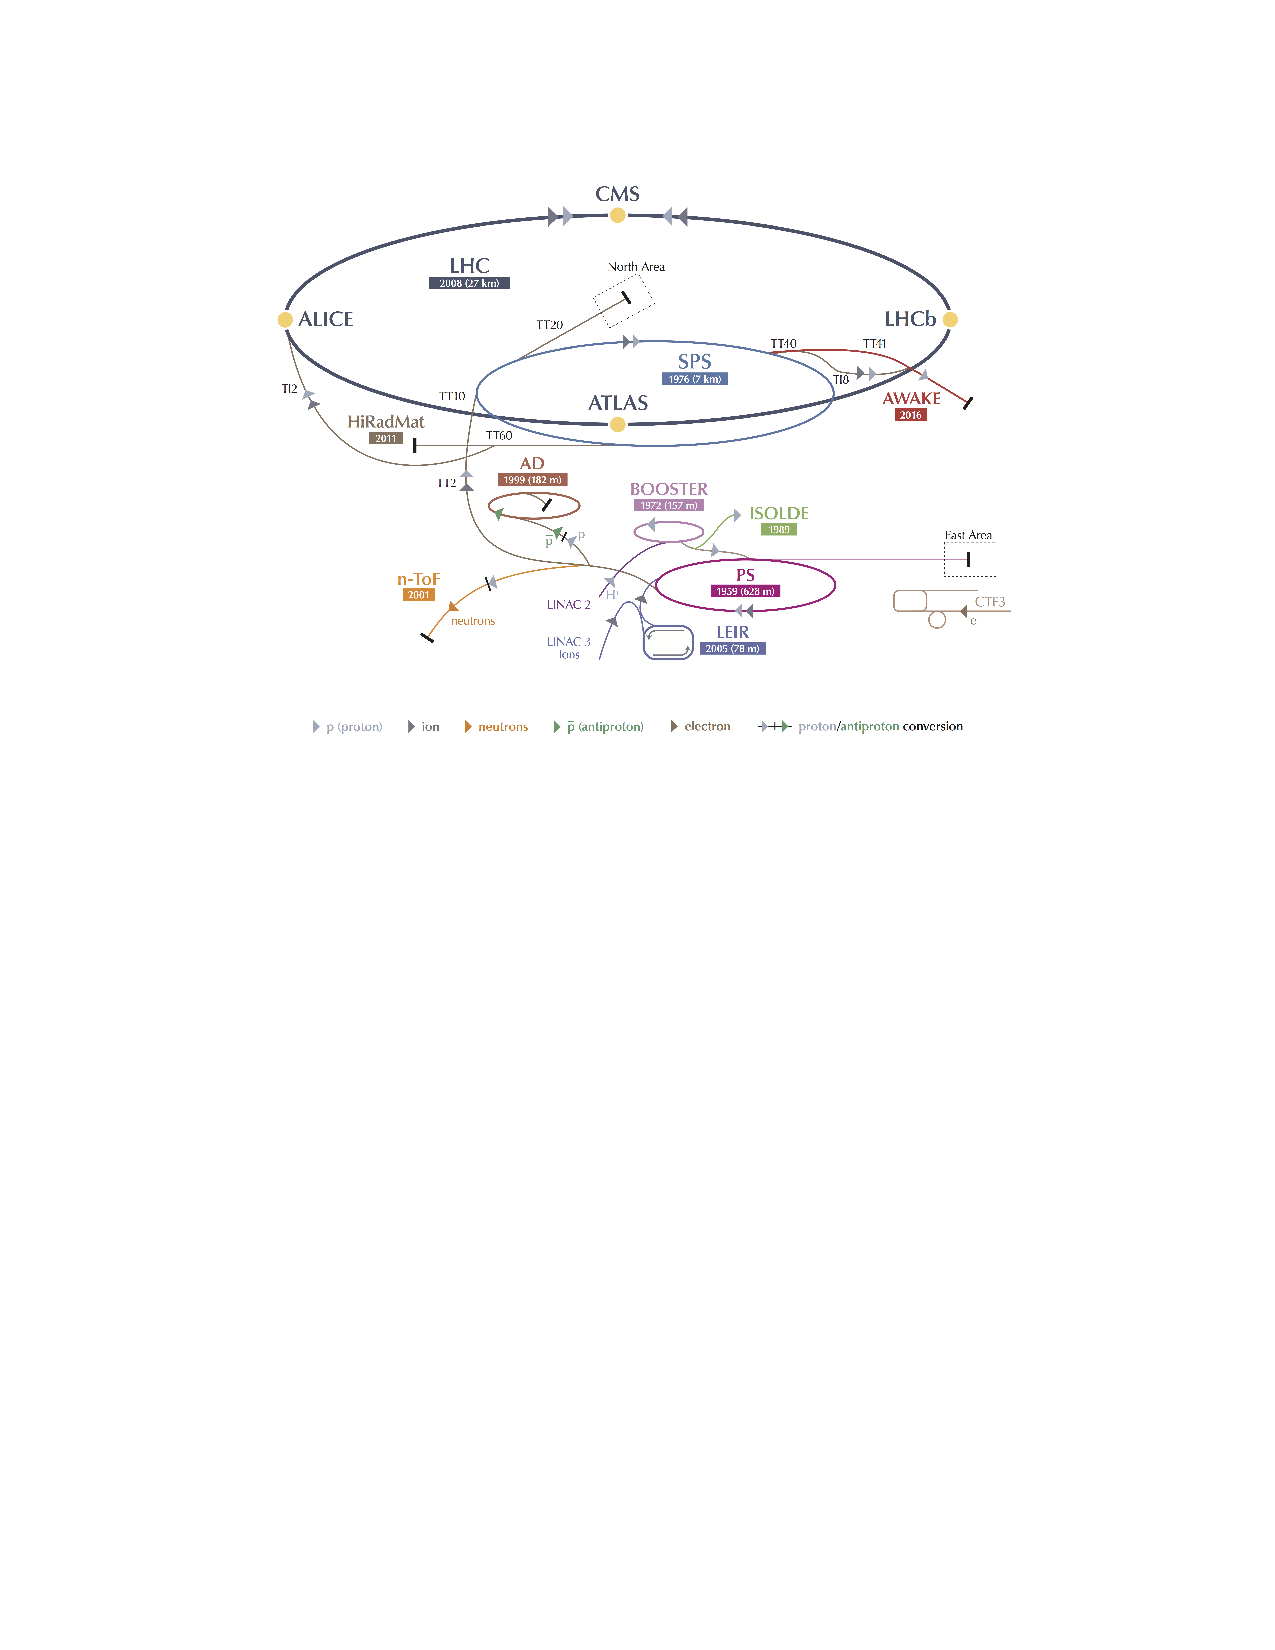
\includegraphics[width=0.9\textwidth]{figures/lhc_protons.pdf}
\caption{Schematic of the CERN accelerator complex.}
\label{fig:lhc}
\end{figure}


\section{The CMS detector}

CMS was designed with the following requirements in mind (in no particular order):
\begin{itemize}
\item Good muon identification and momentum resolution over a wide range of momenta and
angles, good dimuon mass resolution (1\% at 100 GeV), and the ability to determine unambiguously
the charge of muons with p < 1 TeV
\item Good charged-particle momentum resolution and reconstruction efficiency in the inner
tracker. Efficient triggering and offline tagging of $\tau$'s and b-jets, requiring pixel detectors
close to the interaction region
\item Good electromagnetic energy resolution, good diphoton and dielectron mass resolution (1\% at 100 GeV),
wide geometric coverage, ${\pi}^{0}$ meson rejection, and efficient photon and lepton
isolation at high luminosities
\item Good missing transverse energy and dijet mass resolution, requiring hadron calorimeters
with a large hermetic geometric coverage and with fine lateral segmentation
\end{itemize}

\begin{figure}[hb]
\centering
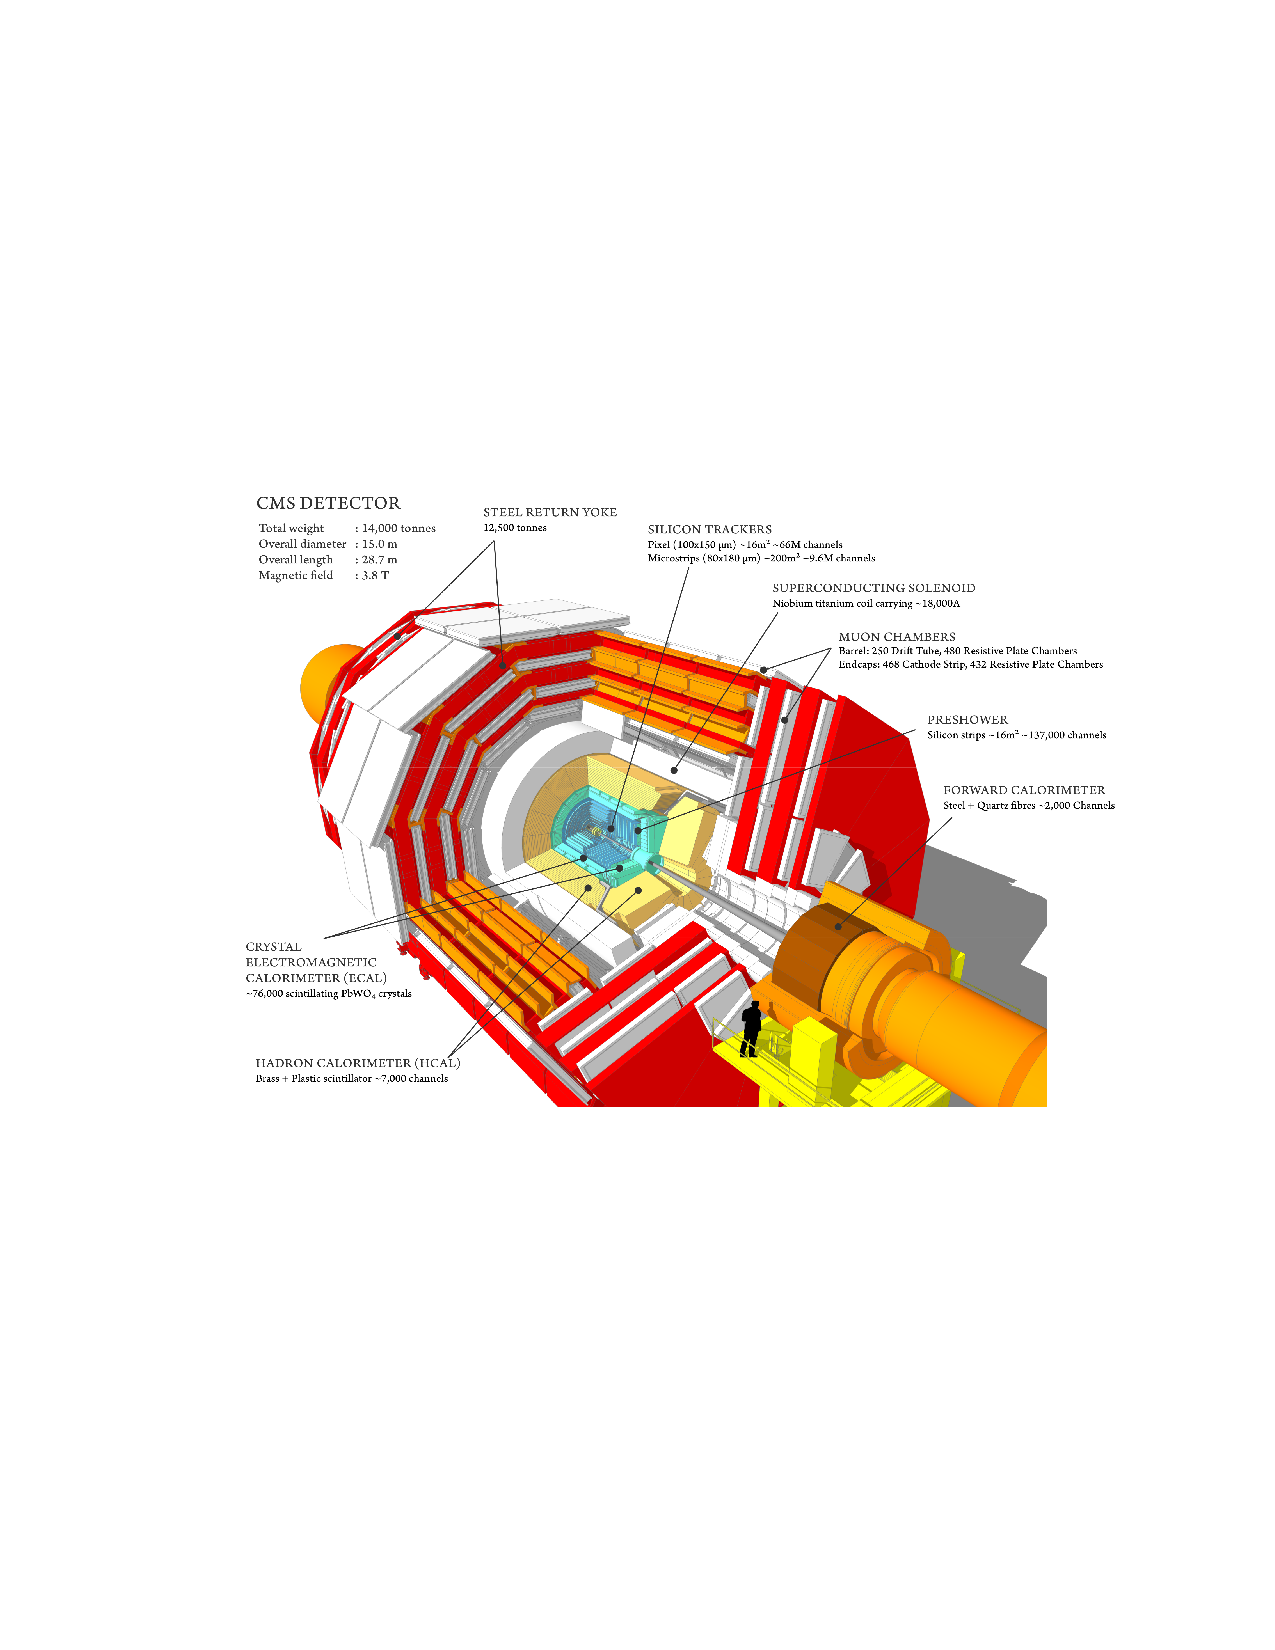
\includegraphics[width=0.95\textwidth]{figures/cms_detector.pdf}
\caption{Schematic of the CMS detector.}
\label{fig:cmsdetector}
\end{figure}

The central feature of the CMS apparatus is a superconducting solenoid of 6 m internal diameter, providing a magnetic field of 3.8 T.
Within the solenoid volume are a silicon pixel and strip tracker, a lead tungstate crystal electromagnetic calorimeter (ECAL), and a brass and scintillator hadron calorimeter (HCAL), each composed of a barrel and two endcap sections. 
Forward calorimeters extend the pseudorapidity coverage provided by the barrel and endcap detectors. 
Muons are detected in gas-ionization chambers embedded in the steel flux-return yoke outside the solenoid.

Events of interest are selected using a two-tiered trigger system~\cite{Khachatryan:2016bia}.
The first level, composed of custom hardware processors, uses information from the calorimeters and muon detectors to select events at a rate of around 100 kHz within a time interval of less than 4 $\mu$s.
The second level, known as the high-level trigger, consists of a farm of processors running a version of the full event reconstruction software optimized for fast processing, and reduces the event rate to around 1 kHz before data storage.

\subsubsection{Coordinate system}
To describe location, CMS uses a standard right-handed Cartesian coordinate system where 
the $x$ direction points to the center of the LHC ring, 
the $y$ direction points to the sky,
and the $z$ direction points in the counterclockwise beam direction at the interaction point.
This is used for locating interaction vertices and tracks' impact parameters with respect to those vertices.
However, this work will also frequently use a set of modified spherical coordinates $(r,\phi,\eta)$
which are conventional in particle physics.
Here, $r$ is the radial coordinate, $\phi$ is the azimuthal angle, and $\eta$ is the \textit{pseudorapidity}, given by
\begin{equation}
\eta  \equiv {-} \mathrm{ln}\:\mathrm{tan}\:\frac{\theta}{2} \implies \theta \equiv 2\:\mathrm{arctan} \left(e^{-\eta}\right)
\label{eq:eta}
\end{equation}
where $\theta$ is the polar angle. 
In these coordinates, the transverse momentum $p_T$ of a particle is related to its total momentum $|\vec{p}|$ and the hyperbolic secant of pseudorapidity as
\begin{equation}
p_T = |\vec{p}|~\mathrm{sech}~\eta
\end{equation}

A variable used to denote the angular separation between two objects in the detector is $\Delta R$,
which is defined as
\begin{equation}
\Delta R = \sqrt{(\phi_1-\phi_2)^2 + (\eta_1-\eta_2)^2}
\end{equation}

\subsection{Trackers}

The inner tracking system of CMS is designed to provide a precise and efficient measurement
of the trajectories of charged particles emerging from the LHC collisions, as well as a precise
reconstruction of secondary vertices. It surrounds the interaction point and has a length of 5.8 m
and a diameter of 2.5 m. The CMS solenoid provides a homogeneous magnetic field of 4 T over
the full volume of the tracker.

At the LHC design luminosity of 1034 cm\textsuperscript{-2} s\textsuperscript{-1},
there are on average about 1000 particles from more than 20 overlapping proton-proton interactions traversing
the tracker for each bunch crossing, i.e. every 25 ns. Therefore, a detector technology featuring high
granularity and fast response is required, such that the trajectories can be identified reliably and
attributed to the correct bunch crossing. However, these features imply a high power density of
the on-detector electronics which in turn requires efficient cooling. This is in direct conflict with
the aim of keeping to the minimum the amount of material in order to limit multiple scattering,
bremsstrahlung, photon conversion, and nuclear interactions. Thus, the design was optimized to balance these competing needs.

The intense particle flux will also cause severe radiation damage to the tracking system.
The main challenge in the design of the tracking system was to develop detector components able
to operate in this harsh environment for an expected lifetime of 10 years. These requirements on
granularity, speed and radiation hardness lead to a tracker design entirely based on silicon detector
technology. The CMS tracker is composed of a pixel detector with three barrel layers at radii
between 4.4 cm and 10.2 cm and a silicon strip tracker with 10 barrel detection layers extending
outwards to a radius of 1.1 m. Each system is completed by endcaps which consist of 2 disks in
the pixel detector and 3 plus 9 disks in the strip tracker on each side of the barrel, extending the
acceptance of the tracker up to a pseudorapidity of $|\eta| < 2.5$. With about 200 m\textsuperscript{2} of active silicon
area the CMS tracker is the largest silicon tracker ever built.

\begin{figure}[hbtp]
\centering
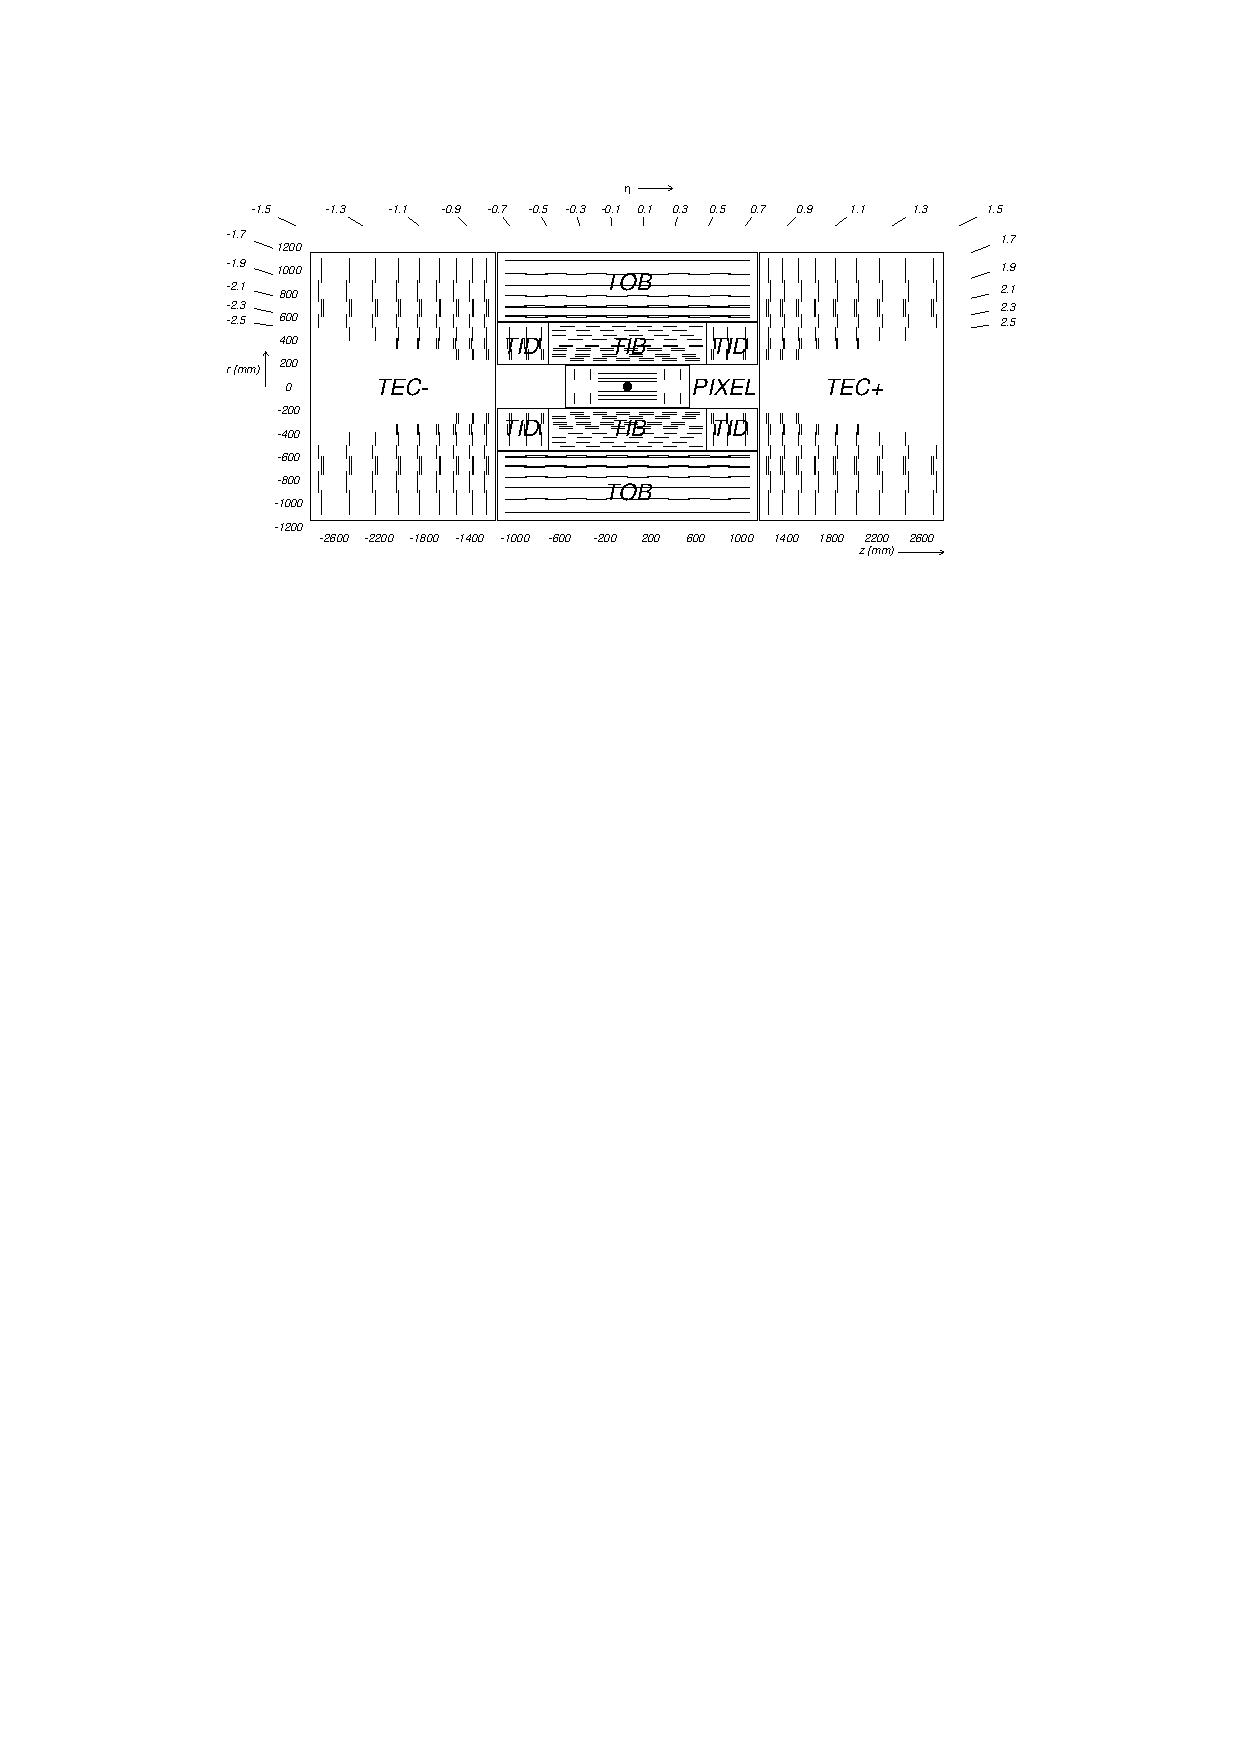
\includegraphics[width=0.9\textwidth]{figures/cms_tracker.pdf}
\caption{Layout of the CMS tracker. From \cite{Chatrchyan:2008aa}.}
\label{fig:cms_tracker}
\end{figure}

\subsection{Electromagnetic calorimeter}
The electromagnetic calorimeter of CMS (ECAL) is a hermetic homogeneous calorimeter made of
61,200 lead tungstate ($\textrm{PbWO}_{\textrm{4}}$) crystals mounted in the central barrel part,
and 7,324 crystals in each of the two endcaps. 
A preshower detector is placed in front of the endcap crystals.
Avalanche photodiodes (APDs) are used as photodetectors in the barrel and vacuum phototriodes
(VPTs) in the endcaps. The use of high density crystals has allowed the design of a calorimeter
which is fast, has fine granularity and is radiation resistant, all important characteristics in the LHC
environment. 
One of the driving criteria in the design was the capability to detect the decay to two
photons of the postulated Higgs boson.
This capability is enhanced by the good energy resolution
provided by a homogeneous crystal calorimeter.

\begin{figure}
\centering
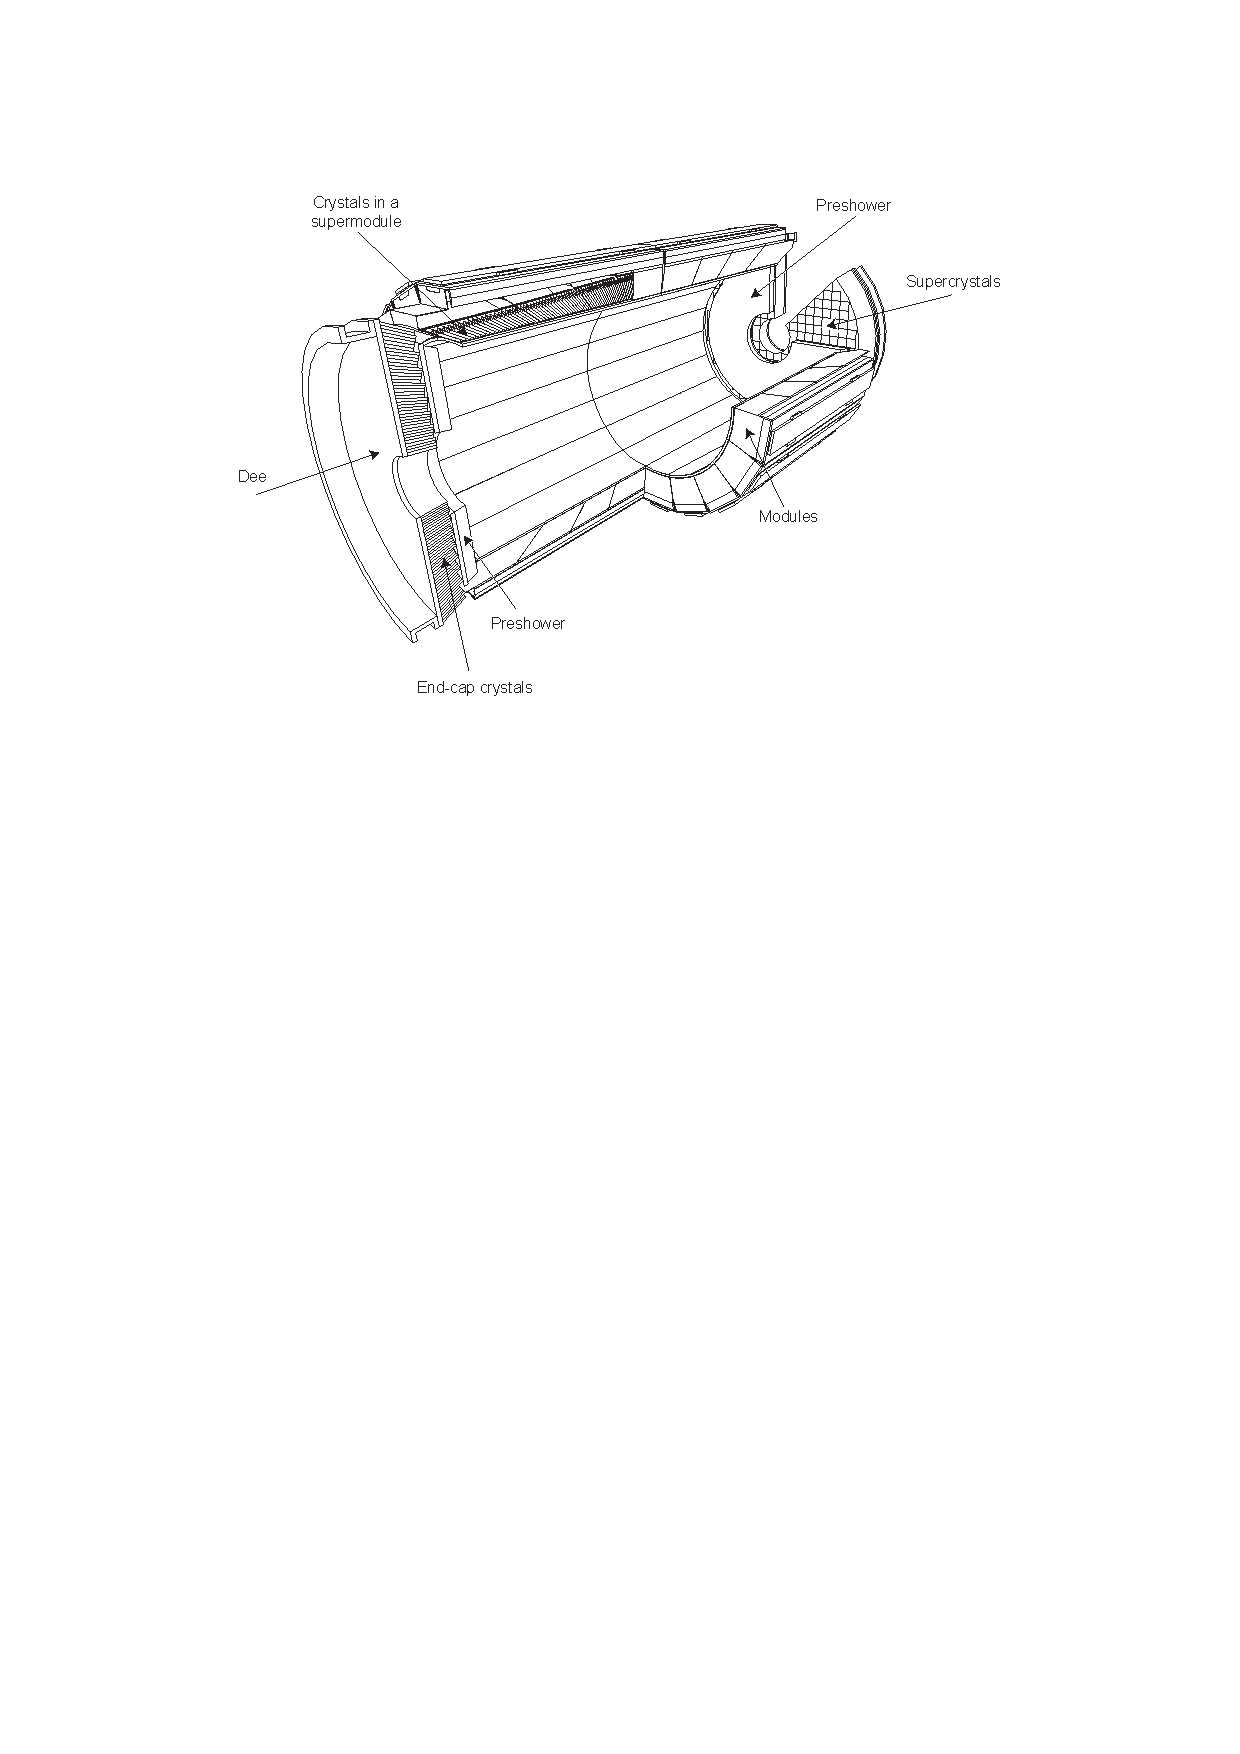
\includegraphics[width=0.9\textwidth]{figures/ecal_layout.pdf}
\caption{Layout of the CMS electromagnetic calorimeter showing the arrangement of crystal
modules, supermodules and endcaps, with the preshower in front. From \cite{Chatrchyan:2008aa}.}
\label{fig:ecal_layout}
\end{figure}

The number of scintillation photons and the electronic amplification thereof both are decreasing with temperature. 
So the ECAL must be kept at a stable temperature of $18\pm0.05$\textdegree~ C.
Water cooling and aluminum tubing are used to meet this need.

\subsubsection{ECAL barrel}
The ECAL barrel (EB) covers the pseudorapidity range $|\eta|<1.479$.
The granularity is 360 in $\phi$ and 170 in $\eta$, giving 61,200 crystals in all.
The crystals have a tapered shape.
They are mounted in a quasi-projective geometry to avoid cracks aligned with particle trajectories.
In other words, their central axes are not exactly parallel to a path from the interaction point, 
in either the $\phi$ or $\eta$ projections.
The crystal cross-section corresponds to approximately $0.0174 \times 0.0174$ in $\eta\times\phi$
or $22 \times 22$ mm\textsuperscript{2} at the front face of the crystal--and $26 \times 26$ mm\textsuperscript{2}
at the rear face.
The crystals' radial length is 230 mm, corresponding to 25.8 radiation lengths.

\begin{figure}
\centering
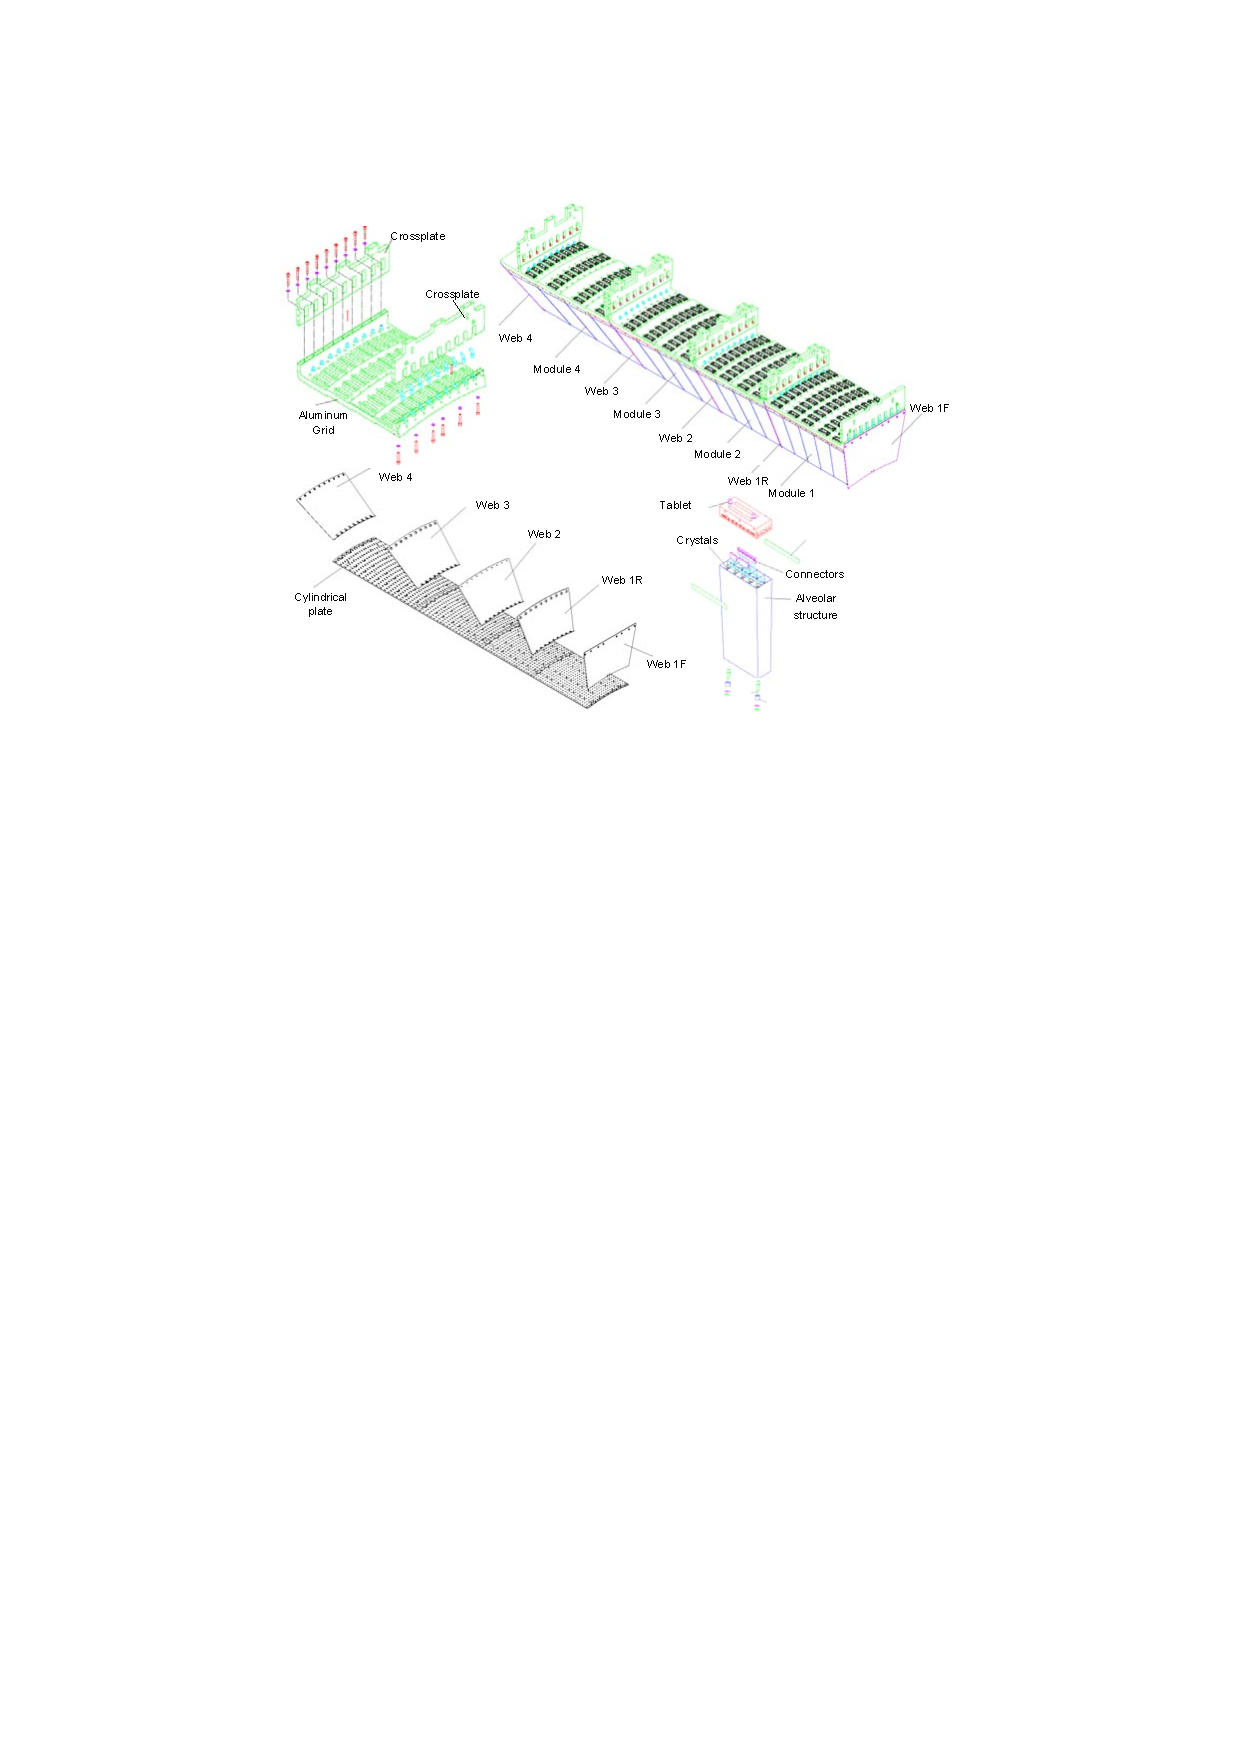
\includegraphics[width=0.9\textwidth]{figures/ecal_barrel.pdf}
\caption{Layout of the ECAL barrel. From \cite{Chatrchyan:2008aa}.}
\label{fig:ecal_barrel}
\end{figure}

In the barrel, the scintillation photons are collected by Hamamatsu type S8148 reverse structure avalanche photodiodes.
Their active area is $5\times5$ mm\textsuperscript{2}. Two are mounted on each crystal.

\subsubsection{ECAL endcaps}
The ECAL endcaps (EE) cover the rapidity range $1.479 < \eta < 2.5$.
The distance from the interaction point and the endcaps is 315.4 cm with the 4 T magnetic field on.
Most of each endcap consists of identically shaped crystals grouped in mechanical units of $5\times5$ crystals, called supercrystals.
As with the EB crystals, the central axes of the EE supercrystals are not exactly parallel to a path from the interaction point. 
The front face of these crystals has an area of $28.62\times28.62$ mm\textsuperscript{2}.
The rear face has an area of $30\times30$ mm\textsuperscript{2}.
The crystals' length is 220 mm or 24.7 radiation lengths.

In the endcaps, the scintillation photons are collected by type PMT188 vacuum phototriodes
from National Research Institute Electron in St. Petersburg.
Their active area is 280 mm\textsuperscript{2}. One is mounted on each crystal.

It is relevant to make a note here that the physical cracks between the EB and EEs exist at $1.4442 < |\eta| < 1.566$. 
This has a negative effect on the electron identification efficiency, to be described in great detail later.
This motivates the non-intuitive kinematic binnings in $\eta$ which are used later
in Chapter~\ref{chap:efficiency} and Appendix~\ref{app:efficiency}.

\subsection{Hadron calorimeters}
The hadron calorimeters (HCALs) exist to measure the energy of hadrons and hadronic jets.
Most hadrons pass through the ECAL due to its limited stopping power and then deposit the rest of their energy in the HCAL.
Muons, and the few energetic hadrons which punch through the HCAL, traverse past it and reach the muon system.
From the visible particle energies recorded in the ECAL, HCAL, and muon systems, 
it is possible to construct the quantity of missing transverse energy in order to
infer the production of neutrinos or exotic particles.
Figure~\ref{fig:hcalslice} shows the longitudinal view of the CMS detector. The dashed lines are at fixed $\eta$ values. 
The hadron calorimeter barrel and endcaps sit behind the tracker and the electromagnetic
calorimeter as seen from the interaction point. The hadron calorimeter barrel is radially restricted
between the outer extent of the electromagnetic calorimeter (R = 1.77 m) and the inner extent of
the magnet coil (R = 2.95 m). This constrains the total amount of material which can be put in
to absorb the hadronic shower. Therefore, an outer hadron calorimeter or tail catcher is placed
outside the solenoid complementing the barrel calorimeter. Beyond $|\eta| = 3$, the forward hadron
calorimeters placed at 11.2 m from the interaction point extend the pseudorapidity coverage down
to $|\eta| = 5.2$ using a Cherenkov-based, radiation-hard technology.
The HCAL subsystems are described briefly below, with more detailed information on the geometry and 
readout being available in~\cite{CMSTDR}.

\begin{figure}
\centering
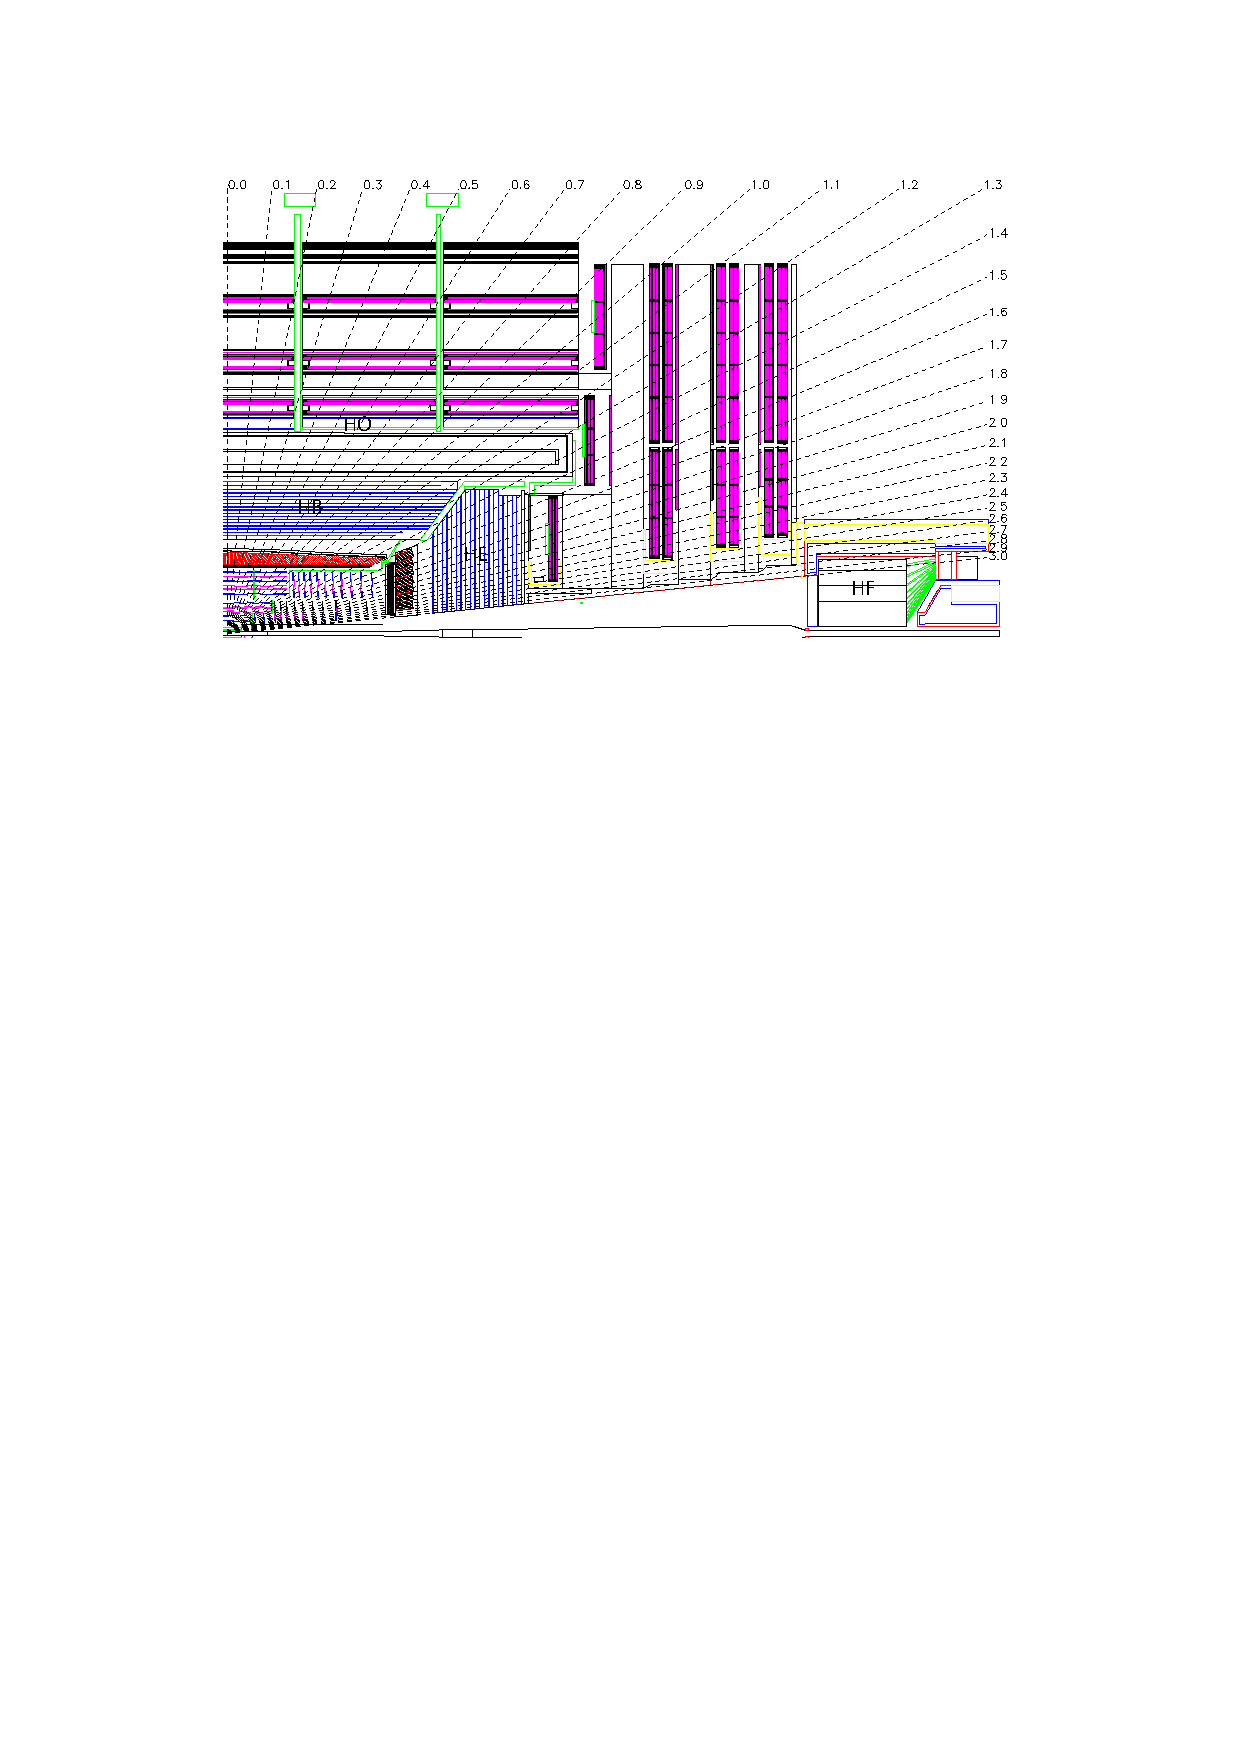
\includegraphics[width=0.98\textwidth]{figures/hcalslice.pdf}
\caption{Longitudinal slice of the CMS detector showing the locations of the hadron barrel
(HB), endcap (HE), outer (HO) and forward (HF) calorimeters.}
\label{fig:hcalslice}
\end{figure}

\subsubsection{HCAL barrel}
The HCAL barrel (HB) is a sampling calorimeter and covers the pseudorapidity range $|\eta| < 1.3$.
It consists of 36 identical azimuthal wedges which form two half-barrels. 
The wedges are constructed out of flat brass absorber plates which are parallel
to the beam axis.  Each wedge is segmented into four azimuthal angle ($\phi$) sectors. 
The innermost and outermost plates are made of stainless steel for structural strength.

The absorber consists of a front steel plate 40 mm thick,
followed by eight 50.5 mm thick brass plates, six 56.5 mm thick brass plates,
and a 75 mm thick steel back plate.
The last layer is thicker to correct for late developing showers which could leak out the back.
The total absorber thickness at 90\textdegree~is 5.82 interaction lengths ($\lambda_I$).
The HB effective thickness increases with polar angle ($\theta$) as $1/\textrm{sin}\:\theta$,
resulting in 10.6 $\lambda_I$ at $|\eta| = 1.3$. 

The HB baseline active material is 3.7 mm thick Kuraray SCSN81 plastic scintillator, 
chosen for its long-term stability and moderate radiation hardness. 
The first layer of scintillator is located in front of the steel support plate, 
and is made of 9 mm thick Bicron BC408. 
Its purpose is to sample hadronic showers developing in the inert material between
the ECAL barrel and the HCAL barrel.
The plastic scintillator is divided into 16 $\eta$ sectors, resulting in a segmentation of $(\Delta\eta, \Delta\phi) = (0.087, 0.087)$. 

\subsubsection{HCAL endcaps}

The hadron calorimeter endcaps (HE) cover the rapidity range $1.3 < |\eta| < 3$. 
It is designed for high radiation tolerance, in order to survive 10 MRad after 10 years of operation.
The total length of the endcap calorimeter, after the ECAL and HCAL endcaps, is about 10 interaction lengths. 

The absorber is made of C26000 cartridge brass. The material was chosen because it is non-magnetic, has a short interaction length and was available at a relatively low cost.
The absorber is assembled in a staggered geometry which minimizes the cracks between HB and HE and contains no projective dead material. 

The scintillators are of trapezoidal shape and there are 18 layers of them in total. 
The first layer are made of 9 mm thick Bicron BC408. All the rest are made of 3.7 mm thick SCSN81.
The scintillation light is read out via wavelength shifting fibers. 
The granularity of the calorimeters is $(\Delta\eta, \Delta\phi) = (0.087, 0.087)$ for $|\eta| < 1.6$ and $(\Delta\eta, \Delta\phi) = (0.170, 0.170)$ for $|\eta| \geq 1.6$.

\subsubsection{HCAL outer}
The combined stopping power of the ECAL and HCAL barrels does not provide adequate stopping
power in the central region $|\eta| < 1.3$. This is problematic for the missing energy resolution.
To further measure and contain these showers, the hadron calorimeter is extended outside the solenoid with a tail catcher called the HO. Only 40 mm of space in the radial direction is available, 
24 mm of which is used for aluminum honeycomb support structures.

The scintillator plates of the HO are made of 10 mm thick Bicron BC408. There are 5 rings in $\eta$, each of those rings having 12 identical $\phi$ sectors, and each of those sectors having 6 azimuthal slices.
The sizes and positions of the tiles in HO are supposed to roughly map the layers of HB
to make towers of granularity $(\Delta\eta, \Delta\phi) = (0.087, 0.087)$.

The magnetic solenoid coil is used as an additional absorber equal to $1.4/\textrm{sin}\:\theta$ interaction lengths.
Outside the vacuum tank, the magnetic field is returned through an iron yoke roughly 20 mm thick, with 5 rings corresponding to the scintillator plates.
The central ring has scintillators both inside and outside of the iron yoke ring.
The others have scintillators only outside their yoke rings.
All told, the total depth of the calorimeter system is extended to a minimum of
$11.8\:\lambda_I$ except at the barrel-endcap boundary region at around $|\eta|=1.4$.

\subsubsection{HCAL forward}
The forward calorimeter, or HF, exists in an extremely hostile environment. 
At $|\eta|=5$ we expect to have delivered 10 MGy after 10 years of operation.
The active material is fused-silica core, polymer hard-cladded quartz fibers, which have sufficient radiation hardness.
These fibers measure 600 $\pm$ \SI{10}{\micro\meter} in diameter for the fused-silica core,
$ {630}^{+5}_{-10}$ \SI{}{\micro\meter} with the polymer hard-cladding, 
and 800 $\pm$ \SI{30}{\micro\meter} with the protective acrylate buffer.

The geometry consists of a steel absorber structure composed of 5 mm thick grooved
plates. Fibers are inserted in these grooves.
The detector is functionally subdivided into two longitudinal segments. 
Half of the fibers run over the full depth of the absorber (165 cm $\approx 10\:\lambda_I$)
while the other half starts at a depth of 22 cm from the front of the detector.
These two sets of fibers are read out separately. 
This arrangement makes it possible to distinguish showers generated by electrons and photons,
which deposit the majority of their energy in the first 22 cm,
from those generated by hadrons, which produce nearly equal signals in both calorimeter segments on average. 
The absorber has grooves which make a square grid separated by 5.0 $\pm$ 0.1 mm center-to-center, with long and short fibers alternating in the grooves. 

This calorimeter is mostly sensitive to the electromagnetic component of hadronic showers.
Only light that hits the core-cladding interface at an angle larger than the critical angle (71\textdegree) contributes to the calorimeter signal in the form of Cherenkov light. 
After the quoted 10 MGy dose has accumulated over the HF lifetime, the optical transmission of the fibers is reduced just by a factor of 2.

\subsection{Muon system}
\label{ss:muonsystem}
The CMS muon system is capable of reconstructing the momentum and charge of muons over the entire
kinematic range of the LHC. 
Due to the shape of the CMS solenoid magnet, the muon system has a barrel section and 2 endcap sections.
Three types of gaseous particle detectors are used.
Since the total area of the muon detection planes is around 25,000 $\textrm{m}^2$, the 
detectors were chosen to be inexpensive but reliable.

In the barrel region, rectangular drift tubes (DT) are used, 
since there is little neutron-induced muon background, the magnetic field is uniform,
and the real muon rate is relatively low.
In the endcap regions, there is a high muon rate, high muon background, and a
very nonuniform magnetic field, so cathode strip chambers (CSC) are used there.
The third subsystem is the resistive plate chambers (RPC). Their spatial resolution is relatively poor.
But their fast response and good time resolution are useful for the trigger.
They also help resolve ambiguity in the standalone muon reconstruction,
which only uses information from the muon system.

The DTs and CSCs are each capable of triggering on muon $p_T$ independently of the other detector subsystems.
The $p_T$ resolution of this triggering muon object is 15\% in the barrel and 25\% in the endcap.
For muon $p_T$ up to $200 \GeV$, the DTs and CSCs together can give a standalone momentum resolution of 9\%.
Approaching muon momenta of $1 \TeV$, the standalone momentum resolution is 5\%.
The muon resolution is improved when combined with the tracker information in the Particle Flow algorithm.

Lastly, an alignment system measures the relative positions of the muon detectors amidst the inner tracker to optimize the momentum resolution of muons.

\begin{figure}[hbtp]
\centering
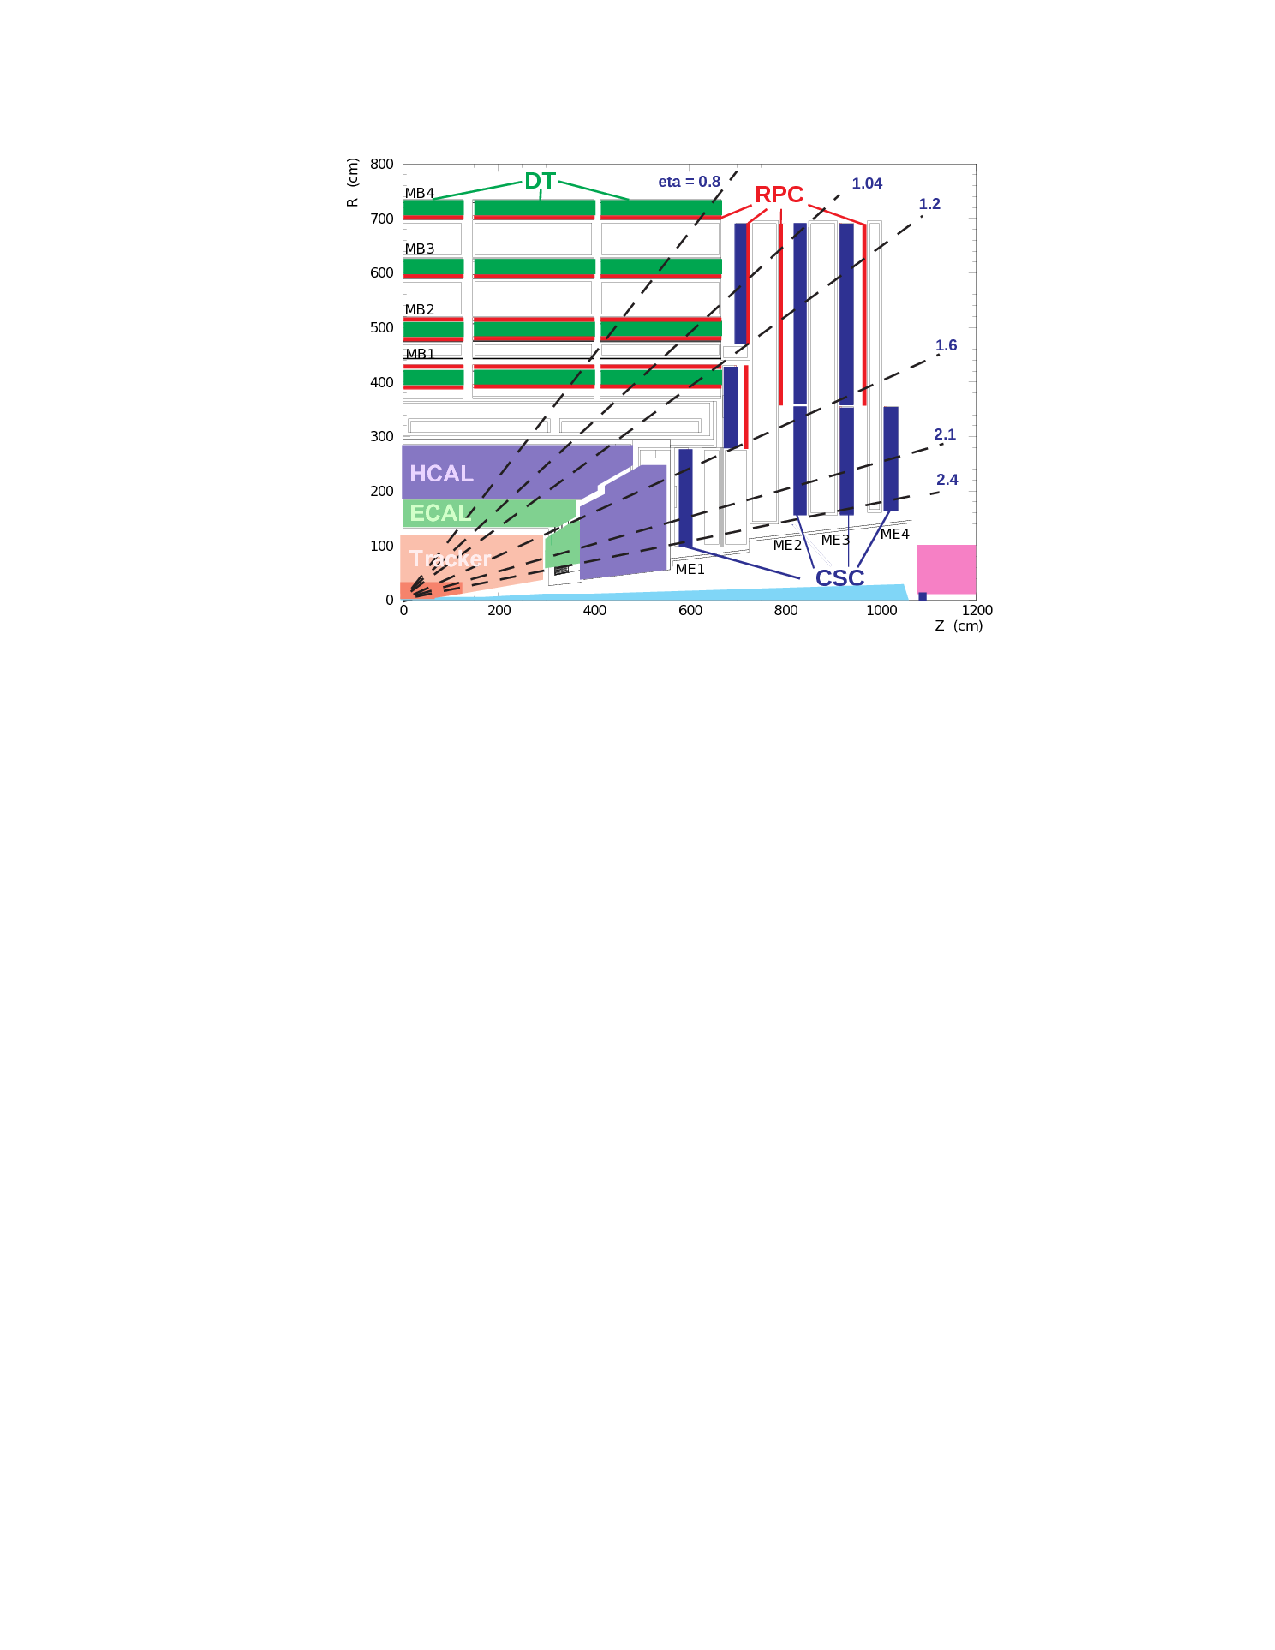
\includegraphics[width=0.8\textwidth]{figures/cms_muon_systems.pdf}
\caption{
Quarter-view of the CMS detector showing the muon system components. 
From \cite{Chatrchyan:2008aa}.
}
\label{fig:muonsystem}
\end{figure}

\subsubsection{Drift tubes}
The DTs cover the pseudorapidity region $|\eta|<1.2$.
There are 4 stations forming concentric cylinders around the beam line.
The 3 inner cylinders have 60 drift chambers each and the outer cylinder has 70.
There are about 172,000 sensitive wires of about 2.4m in length.
The maximum drift path length is 21 mm. In a gaseous admixture of 85\% Ar and 15\% $\mathrm{CO}_2$ the maximum drift time is 380 ns.
This produces a negligible occupancy and permits the use of single-hit electronics.
Meanwhile, the cell size is sufficiently large to keep the number of electronic channels low and affordable.

Each DT chamber is made of 2 or 3 superlayers (SL).
Each SL is made of layers of rectangular drift cells staggered by half a cell.
The wires in the 2 outer SLs are parallel to the beam line and provide a track measurement
in the magnetic bending plane. 
The wires in the inner SL are orthogonal to the beam line and measure the $z$ position.
This innermost SL is not present in the fourth DT station
Thus, a muon first encounters a $\phi$-measuring SL, passes through a honeycomb spacer plate,
then crosses the $z$-measuring SL and the second $\phi$-measuring SL.
Due to discontinuities in the design,
a muon could end up crossing only two stations instead of the maximum four.

One superlayer has time resolution on the order of nanoseconds.
The time measurement is delayed by the drift-time, determined by the design parameters of the drift tubes.
Using the SL information, pattern recognition circuits deliver the position and angle 
of the track segment's center of gravity with precision of 1.5 mm and 20 mrad, respectively.

\begin{figure}[hbtp]
\centering
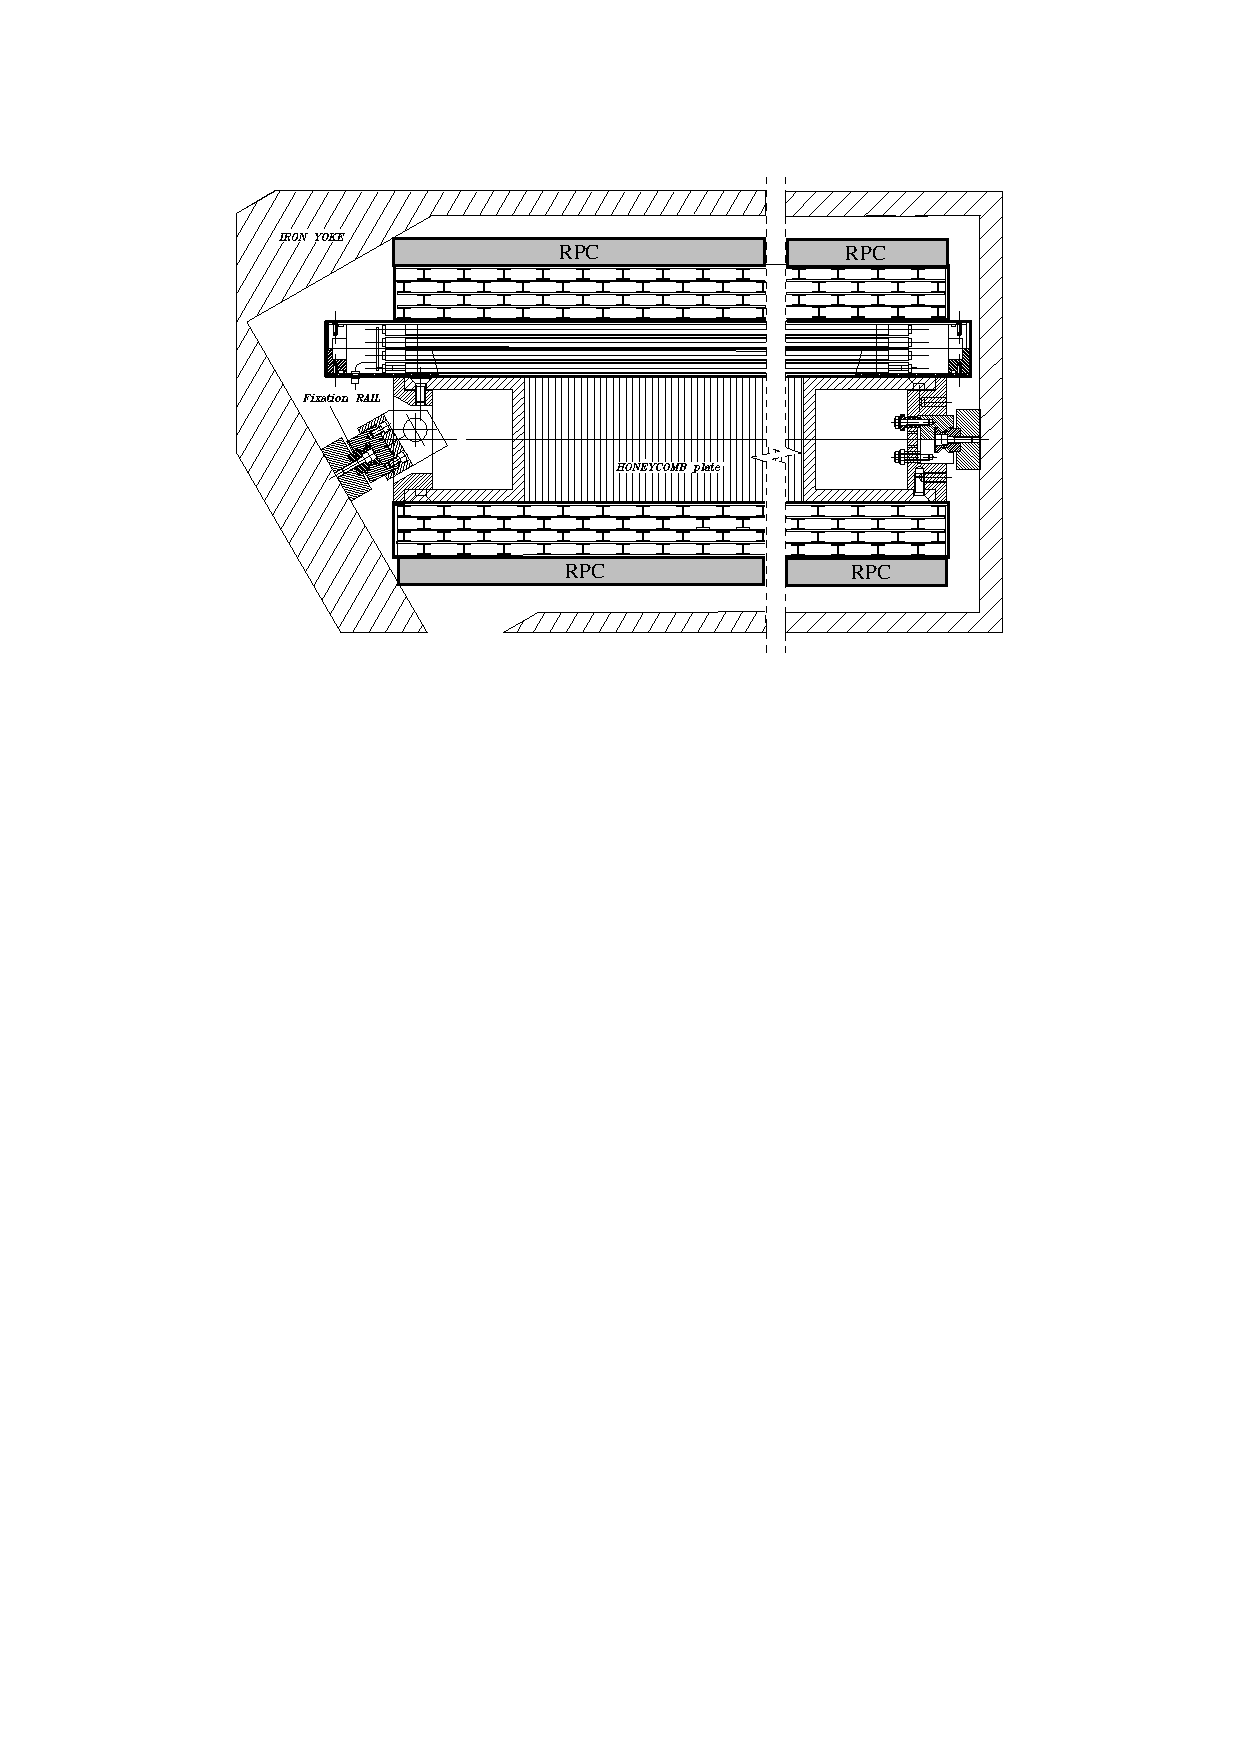
\includegraphics[width=0.80\textwidth]{figures/cms_muonsystem_honeycomb.pdf}
\caption{Chambers of the CMS DT system including the honeycomb support. From \cite{Chatrchyan:2008aa}.}
\label{fig:dt_chambers}
\end{figure}

\begin{figure}[hbtp]
\centering
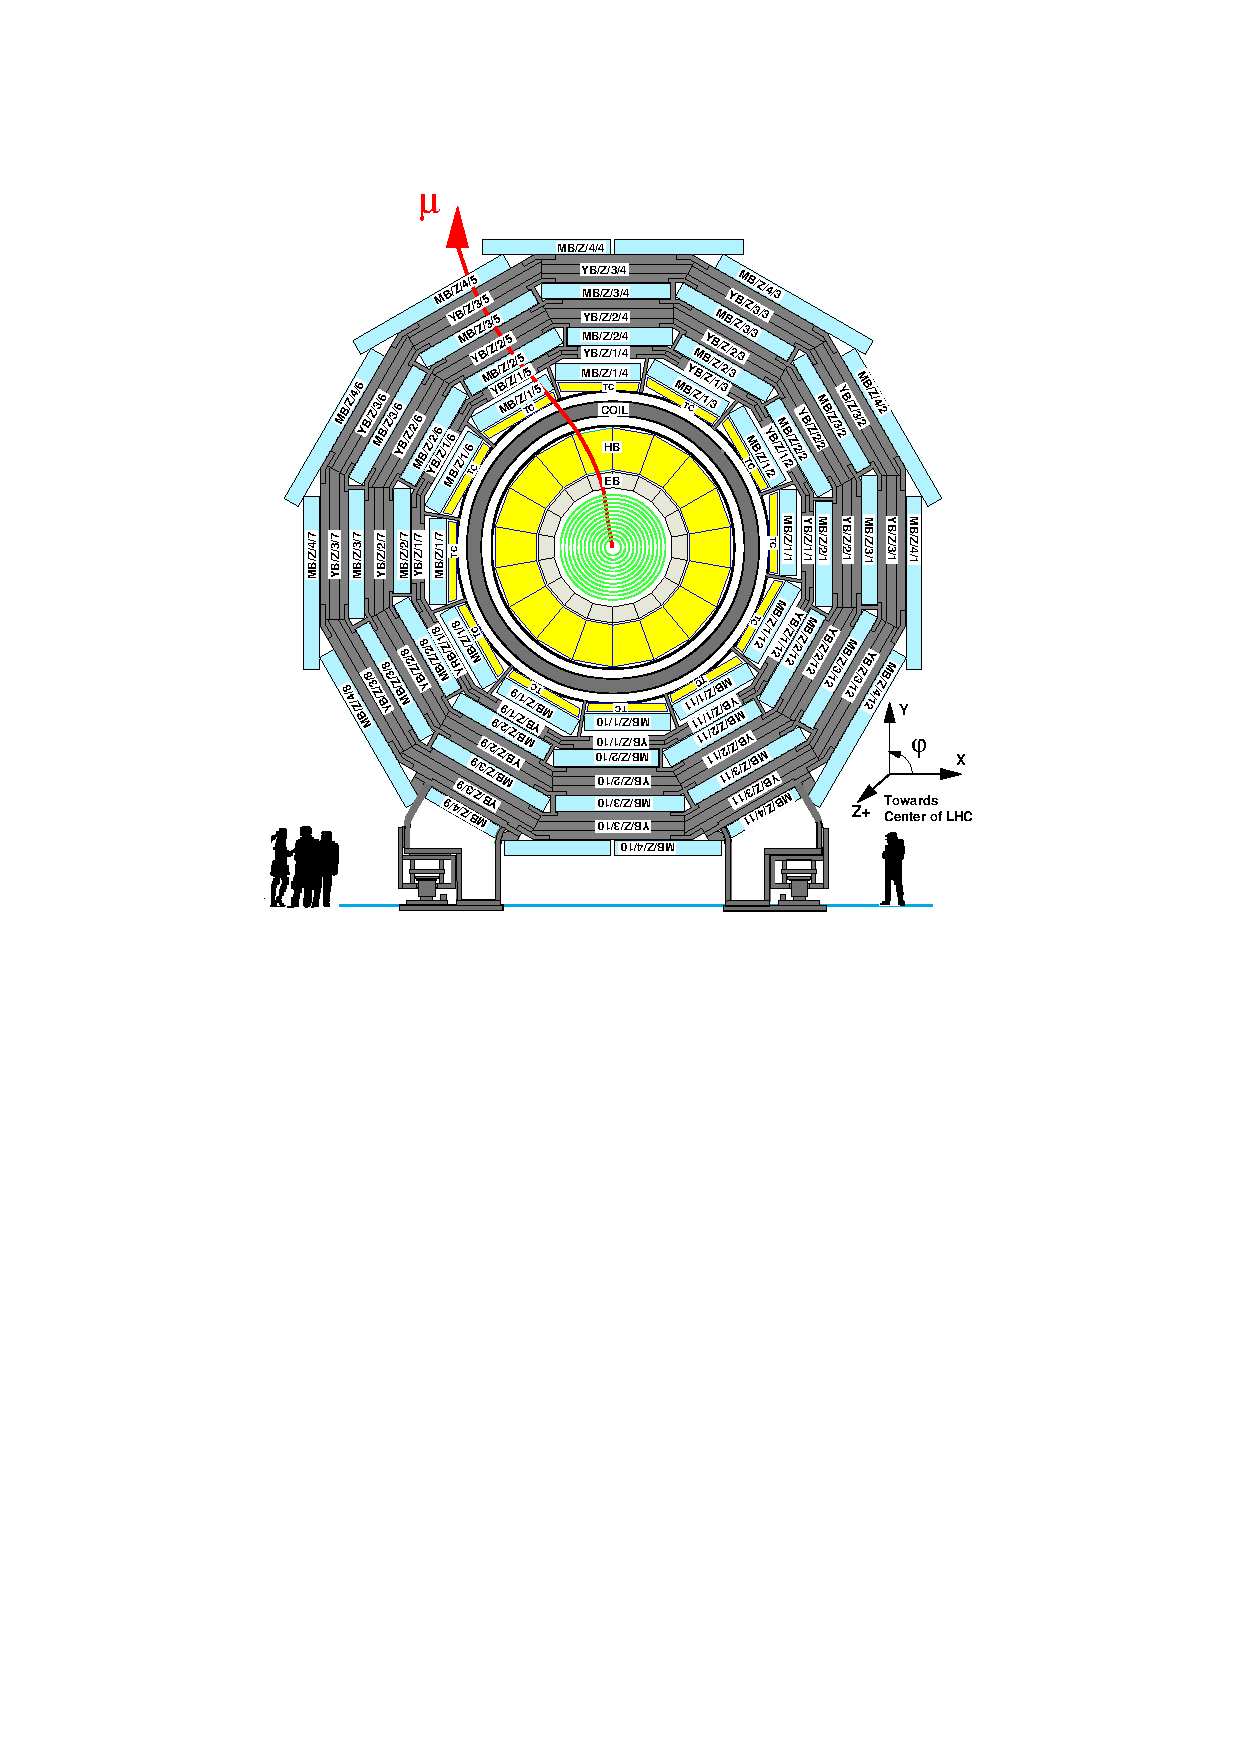
\includegraphics[width=0.8\textwidth]{figures/cms_drifttubes_slice.pdf}
\caption{ Layout of the CMS barrel muon DT chambers in one of the 5 wheels. From \cite{Chatrchyan:2008aa}.}
\label{fig:dt_barrel}
\end{figure}

\subsubsection{Cathode strip chambers}
The CSCs cover the pseudorapidity region $0.9<|\eta|<2.4$.
There are 4 stations of CSCs in each endcap.
The chambers are perpendicular to the beamline and interspersed between the magnetic flux return plates.
The cathode strips point radially outward from the beamline and provide a precision measurement in the $r-\phi$ bending plane.

The CSCs are multiwire proportional chambers comprised of 6 anode wire planes interleaved
among 7 cathode panels. Wires run azimuthally and define a track’s radial coordinate.
Strips are milled on cathode panels and run lengthwise at constant $\Delta\phi$ width. 
The muon coordinate along the wires is obtained by interpolating between charges induced on strips.
The largest chambers, ME2/2 and ME3/2, are about 3.4 × 1.5 m\textsuperscript{2} in size.
The overall area covered by the sensitive planes of all chambers is about 5,000 m\textsuperscript{2},
the gas volume is over 50 m\textsuperscript{3}, and there are about 2 million wires.
There are about 9000 high-voltage channels in the system, 
about 220,000 cathode strip read-out channels with 12-bit signal digitization,
and about 180 000 anode wire read-out channels.

An avalanche on a wire induces charge on a cathode plane.
The charge shape can be approximately parameterized by the Gatti function~\cite{GATTI197983}.
Given the CSC geometry, most of the induced charge is shared among three or four strips.
A strip signal waveform is sampled and digitized every 50 ns.
The overal pulse duration is about 300 ns.
The charge cluster is fit to obtain the spatial coordinate, time, and cluster charge.
Using this method, the spatial resolution for a 6-plane chamber is 80 $\mathrm{\mu m}$.

\begin{figure}[hbtp]
\centering
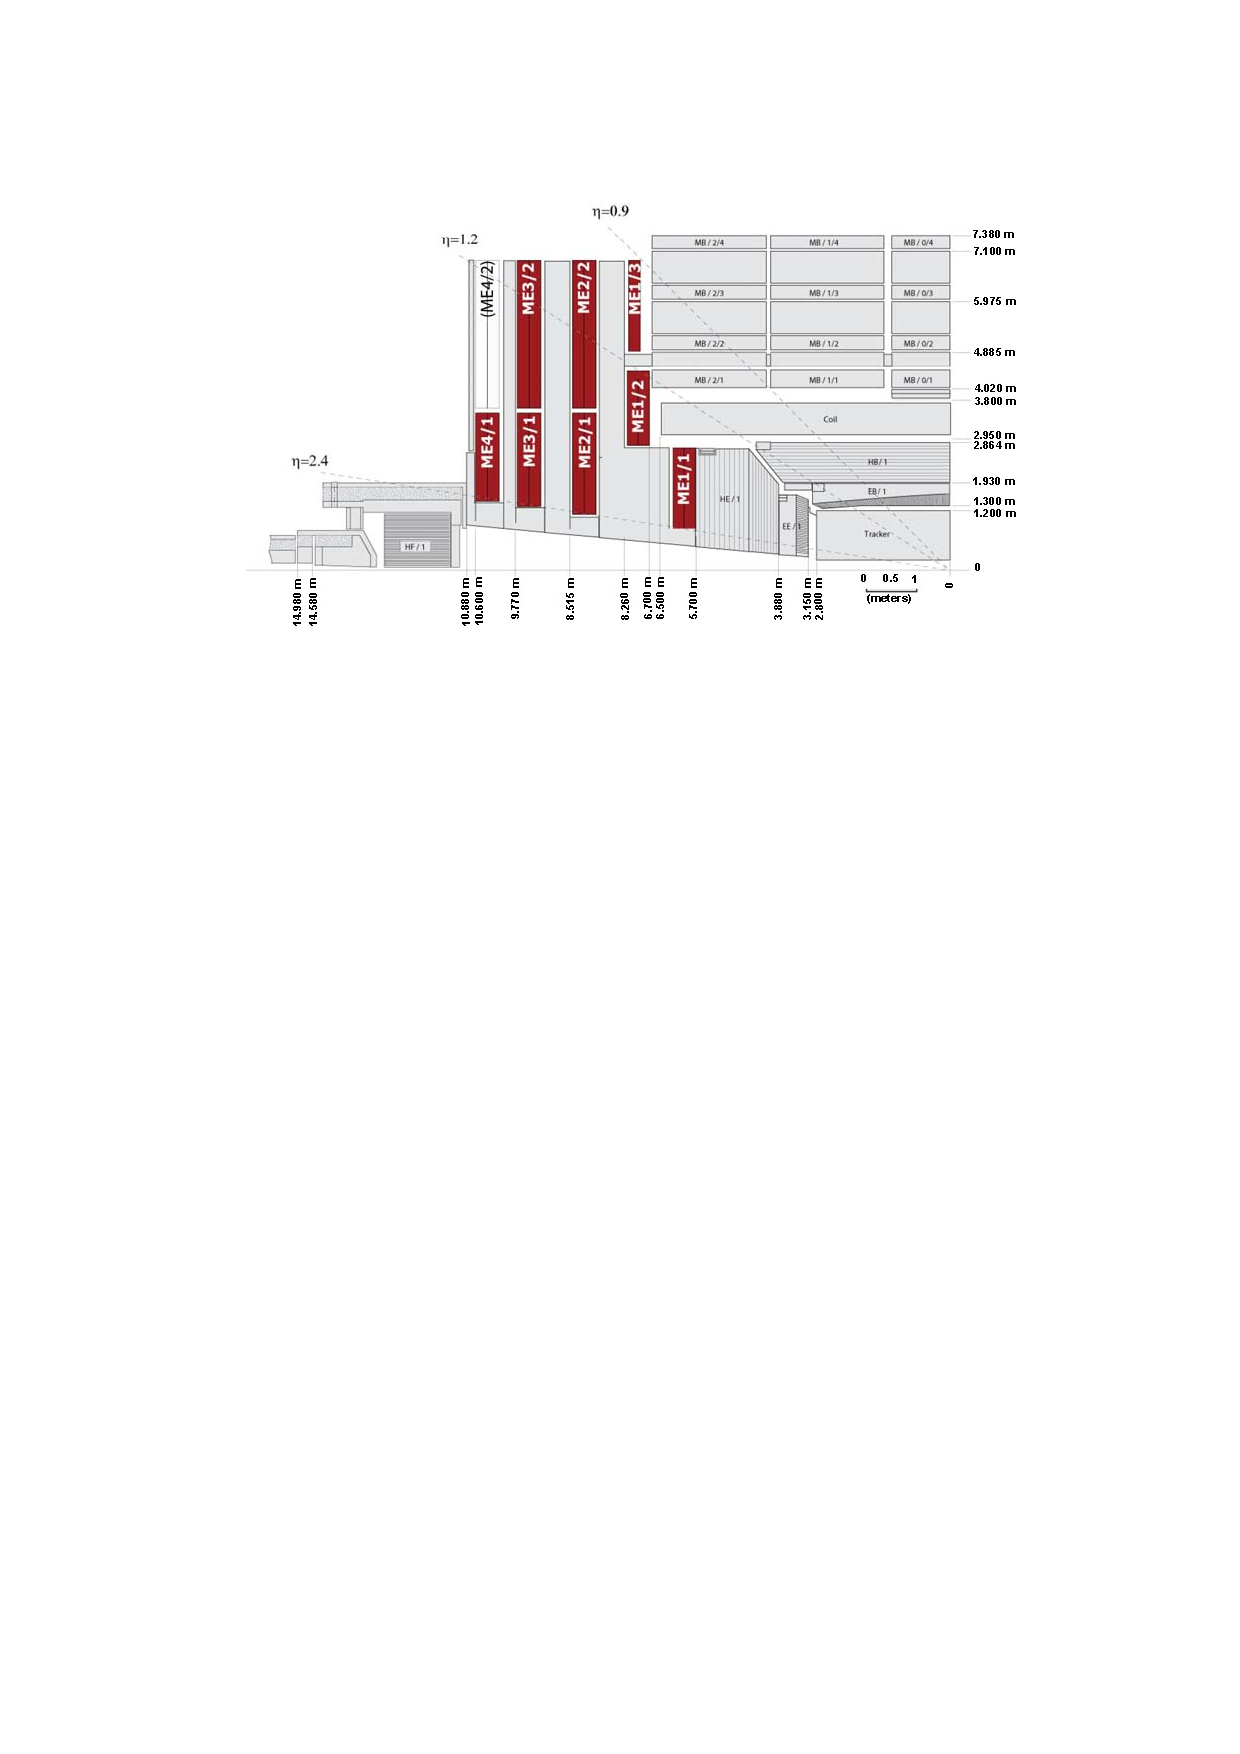
\includegraphics[width=0.8\textwidth]{figures/cms_quarter_csc_red.pdf}
\caption{
Quarter-view of the CMS detector. Cathode strip chambers of the Endcap Muon
system are highlighted.
From \cite{Chatrchyan:2008aa}.
}
\label{fig:cms_quarter_csc_red}
\end{figure}

\begin{figure}[hbtp]
\centering
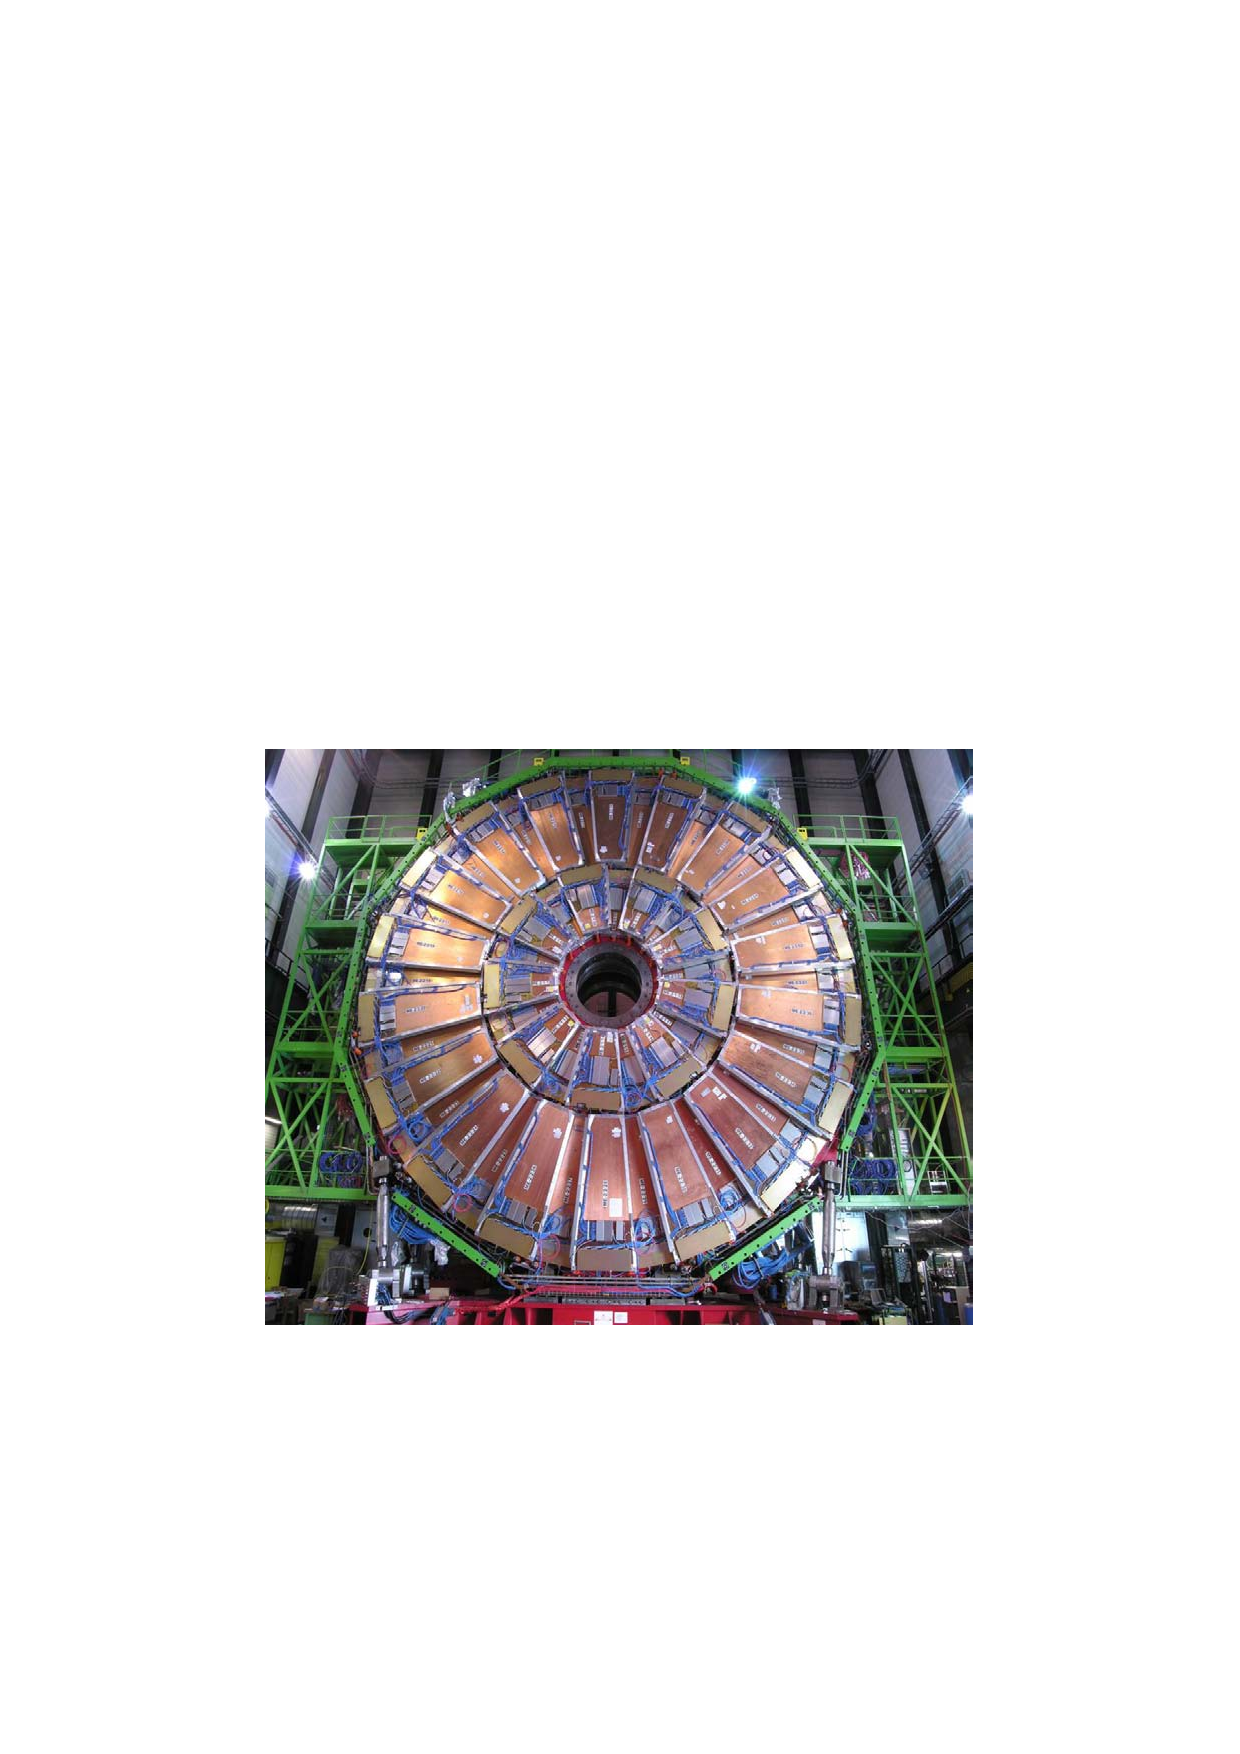
\includegraphics[width=0.8\textwidth]{figures/cms_cscs_me2.pdf}
\caption{
The ME2 station of CSCs. The outer ring consists of 36 ME2/2 chambers, each
spanning 10\degree in $\phi$, and the inner ring of eighteen 20\degree ME2/1 chambers.
The chambers overlap to provide contiguous coverage in $\phi$.
From \cite{Chatrchyan:2008aa}.
}
\label{fig:cms_cscs_me2}
\end{figure}

\subsubsection{Resistive plate chambers}

The RPCs are gaseous parallel-plate detectors with adequate spatial resolution and scintillator-level time resolution.
They are much faster than the 25 ns proton bunch crossing period at the LHC.
Using the RPC information, there is no ambiguity in the association of muon tracks and bunch crossings.

The CMS RPC basic double-gap module consists of two gaps operated in avalanche mode with common
pickup readout strips between them.
The total induced signal is the sum of the two single-gap signals.
Thus, the single-gaps can operate at a lower voltage gap,
with better effective efficiency than a single gap.

In the barrel iron return yoke, the RPC chambers form 6 coaxial sensitive cylinders
that are approximated with concentric dodecagon arrays arranged into 4 stations. See Figure~\ref{fig:cms_rpc_barrel}.

\begin{figure}[hbtp]
\centering
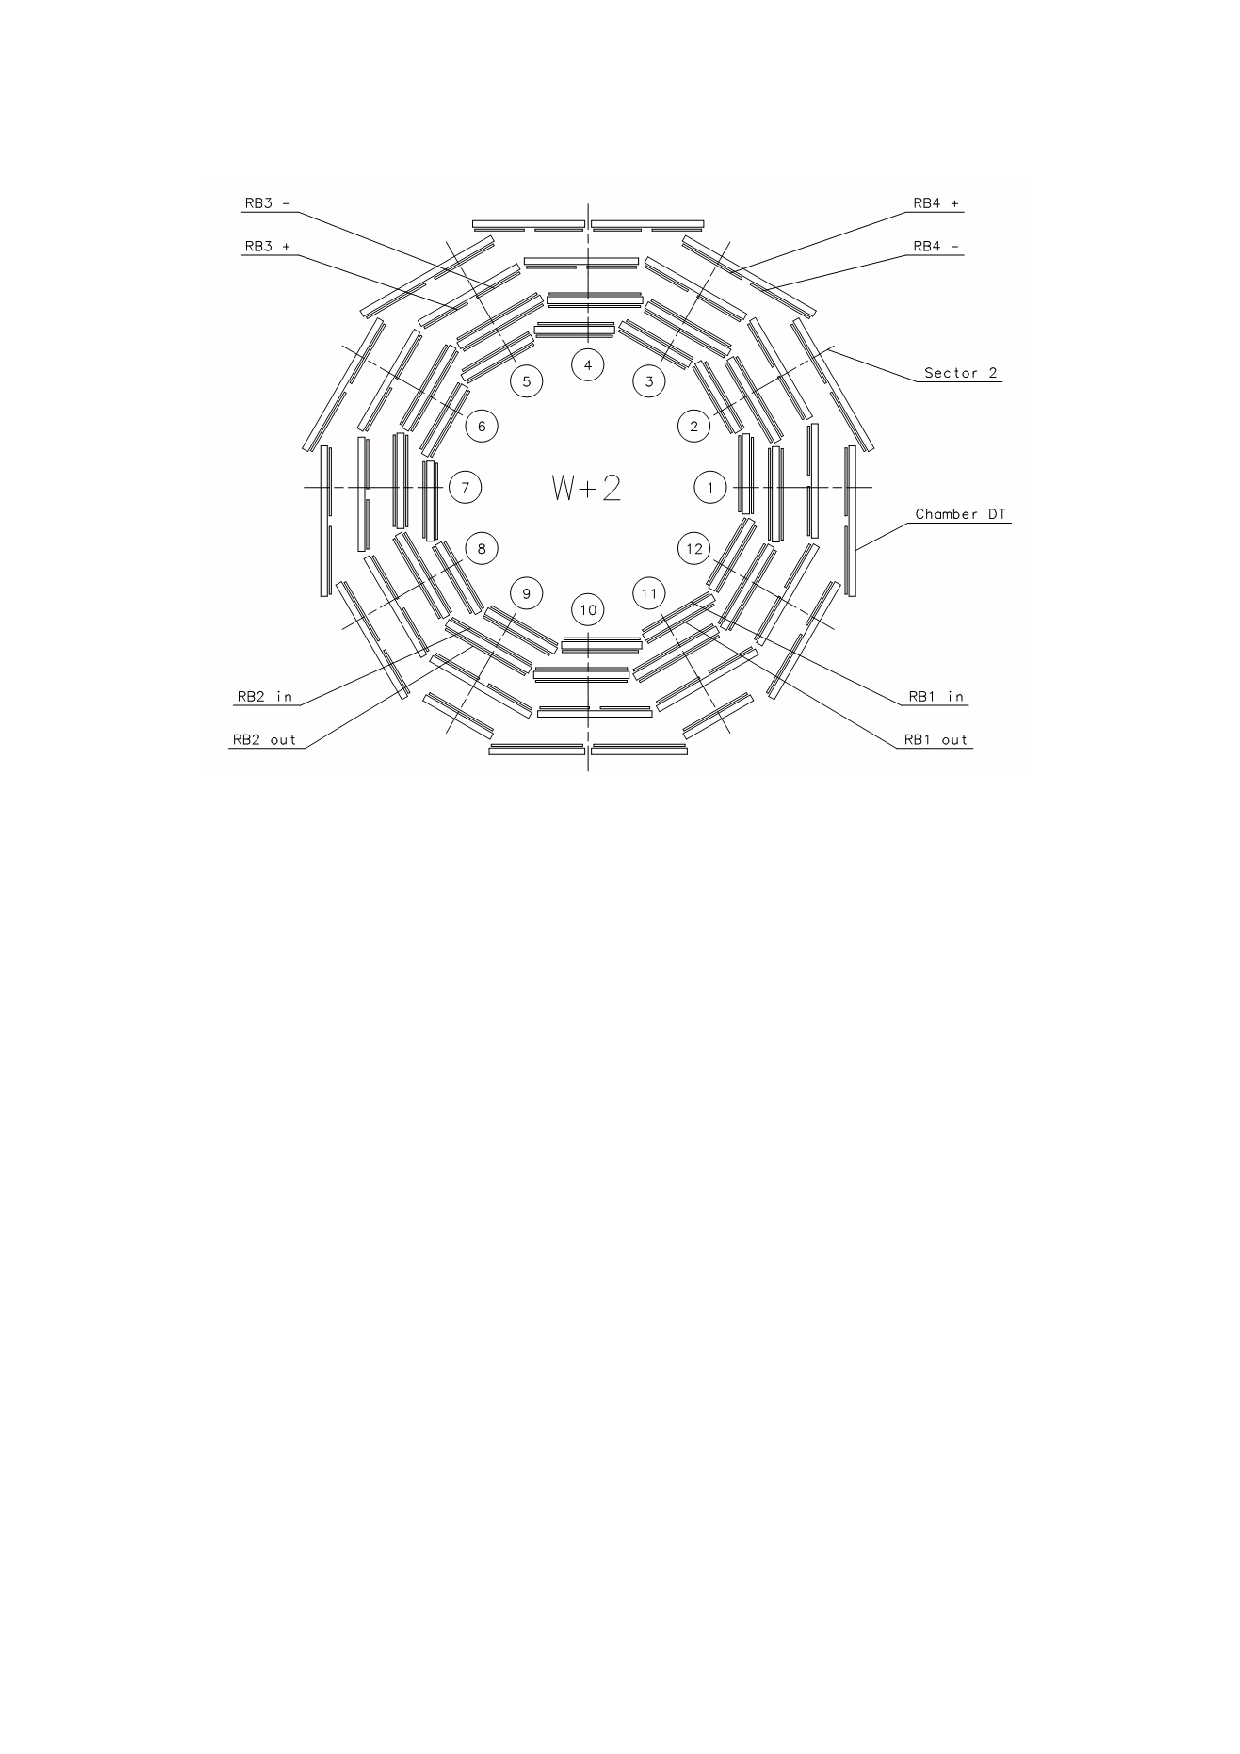
\includegraphics[width=0.8\textwidth]{figures/cms_rpc_barrel.pdf}
\caption{
Schematic layout of one of the 5 RPC barrel wheels. Each wheel is divided into 12 sectors.
From \cite{Chatrchyan:2008aa}.
}
\label{fig:cms_rpc_barrel}
\end{figure}
\clearpage

\subsection{Trigger system}
Triggering algorithms decide which data are recorded in the experiment.
They are implemented in two stages via a combination of hardware and software.

\subsubsection{Level-1 trigger}
The trigger decision process begins with the Level-1 Trigger (L1T) \cite{Khachatryan:2016bia}.  
The hardware implementation of the Level-1 Trigger is in the form of application-specific
integrated circuits (ASICs), field-programmable gate arrays (FPGAs), 
programmable logic devices (PLDs), and random access memory used for memory look-up tables (LUTs).
The FPGAs and LUTs may be reprogrammed, allowing for the algorithms to be revised.

The Level-1 Trigger is subject to a large data flow carried on optical fibers, 
copper cables, and backplanes within hardware crates. 
The data is transmitted in parallel at frequencies which are integer multiples of 40 MHz.
Data events passing the Level-1 Trigger are then transmitted to the so-called ``high-level trigger,'' described next.

\subsubsection{High-Level Trigger}
Data events accepted by the Level-1 Trigger are next processed by the High-Level Trigger (HLT).
Unlike the L1T's readout boards, the HLT is implemented on a commercial Linux computing cluster
called the File-based Filter Farm (F\textsuperscript{3}). There are three types of computing units in the F\textsuperscript{3}:
\begin{itemize}
\item The Readout Units take the information from the readout boards and assemble event fragments from a given detector partition.
\item The Builder Units take the event fragments and assemble full events. The full events are buffered here during the next step.
\item The Filter Units apply the final event selection of the HLT algorithms.
\end{itemize}
The HLT algorithms running on the FUs operate on full-granularity event data
from all subdetector systems. They accept between 1-10\% of events accepted by the L1T.
The algorithms make use of the CMS offline reconstruction framework called CMSSW.

\subsection{Offline world}
Events accepted by the HLT are merged into larger agglomerate files which are stored
locally in a Lustre parallel distributed file system.
Then, they are transferred from the ``online'' CMS experimental site to the
``offline'' CERN Tier-0 computing center at the main CERN campus in Meyrin for processing.
This transfer system is a multithreaded software,
optimized to handle rates of several gigabytes per second during data taking.
Finally, data are distributed worldwide from Tier-0 to the global CMS computing grid for physics studies.

\chapter{Data samples}
\section{The LHC and its proton injection system}


\chapter{Efficiency of lepton trigger, reconstruction, and identification}
\label{chap:efficiency}
%\autoref{chap:efficiency}
After reconstructing leptons in CMS using the information from the detector subsystems,
further offline requirements are applied for the purpose of high quality and low background lepton identification.
The choice of these requirements depends on the analysis, and several well-defined working points are optimized
and released by the relevant Physics Object Groups. The figure of merit for lepton identification is the efficiency,
and the various working points are usually described qualitatively in terms of "tightness,"
with a tighter selection corresponding to lower efficiency and higher purity.
In this note we refer to the whole slew of offline requirements applied to reconstructed leptons under the umbrella term of identification, including quantities such as relative isolation.

Previously, at lower center-of-mass energies, resonant leptonic decays of the $J/\psi$ meson were used to measure lepton identification efficiency.
In Run II at the LHC, we make use of the large cross section of the Z boson resonance and observe its leptonic decays to extract the lepton efficiencies for a wide range of lepton energies and rapidity;
while the $J/\psi$ meson is also still used for efficiency studies at lower transverse momentum.
This chapter describes how the efficiency is measured in data and simulation by studying dilepton events with invariant mass close to the Z boson resonance peak at 91.1876 $\GeV$.
The ensuing discussion presents results for the "Medium 2016" cut-based identification algorithm.

\section{Event selections for the tag-and-probe method}
\label{sec:tnpsel}
The so-called "tag-and-probe" selection consists of a high purity $\dyll$ selection with a
well-identified tag lepton and an oppositre sign probe.
The tag electron (muon) must pass the tight identification, have transverse momentum greater than 30 (25) $\GeV$, 
have $\abs{\eta}<$ 2.5 (2.4), and be matched to the leptonic trigger firing.
The probe electron must have transverse momentum greater than 10 $\GeV$ and $\abs{\eta}<$ 2.5.
For the probe muons, we consider a collection of general tracks. These tracks must have transverse momentum 
greater than 10 $\GeV$, $\abs{\eta}<$ 2.4, and a vertex whose longitudinal position is within 4 cm of that of the tag.

The selection also includes a truth-matching procedure when applied to simulated Drell-Yan samples,
so that all simulated reconstructed dileptons come from leptonic Z decays.
The reconstructed leptons must each have a small angular separation $\Delta R = \sqrt{ \Delta\phi^{2} + \Delta\eta^{2} }$ 
less than 0.3 with a final-state lepton of the same flavor at generator level. For muons, the generator-level and reconstructed
transverse momenta must also be compatible within 10\%.

\subsection{Probe multiplicity calculation}
In order to increase the signal purity of the muon selection, we perform a probe multiplicity calculation to
remove combinatorial background. The track collection as described above is considered, albeit with a 
lowered transverse momentum cut of 3 $\GeV$. Then, the number of opposite sign tag-track pairs having invariant mass above
60 $\GeV$ is counted for each tag; this gives the probe multiplicity. Any muon tags having probe multiplicity
greater than 1 are not considered in the ensuing tag and probe analysis.

\section{Control samples for the lepton efficiencies}
Two independent data samples are chosen to faithfully represent the background distributions for the
tag-and-probe fitting methods. They are defined below.
\label{sec:tnpcontrol}

\subsection{Lepton pion selection}
The mass spectrum of the combinatorial background in the Z selection can be modeled well by selecting
essentially random pairs of tag leptons and charged hadrons whose invariant mass falls within the relevant window.
We select a tag electron (muon) exactly the same as before, along with a PF charged hadron having $\pt>10~\GeV$ and $\abs{\eta}<2.5$
which must originate from the primary event vertex.

The charged hadrons selected in such a way are predominantly but not exclusively pions.
As the CMS detector does not have charged hadron particle ID capabilities beyond $\frac{dE}{dx}$,
which is ineffective for such boosted particles, we have little way of knowing if they are really pions
instead of kaons, protons, or something even more charming.
Thus, we refer to them somewhat ignorantly using $\pi^{\pm}$ as shorthand.

To obtain a data sample orthogonal to the Z selection, and to suppress contamination by Z events,
we remove events from the \ensuremath{\ell^{\pm}\pi^{\pm}} selection with the following cuts:
\begin{itemize}
\item Reject events containing a tag electron (muon) and another reconstructed electron (muon)
\item Reject \ensuremath{\pi^{\pm}} probes with separation $\Delta R$ less than 0.3 with any reconstructed electron or muon
\item Require the same charge assignment for the tag lepton and the pion probe
\end{itemize}

Furthermore, due to low event yields in this selection at higher probe energies for the electron case,
we use an $\eta$-inclusive form of this selection to build the shapes that are used in each bin of probe $\eta$ for probes with $p_{T} > 50~\GeV$.

The \ensuremath{\ell^{\pm}\pi^{\pm}} selection is effective at modeling the background combinatorics, largely
arising from QCD and the W+jets process. However, it fails to accurately
model the lower energy contribution from the non-resonant background processes e.g. $\ttbar \to 2\ell 2\nu 2b$ and $\dytt$.
\subsection{Electron muon selection}
The Z(ee) background can also be modeled by selecting a muon tag along with an electron probe.
In this case, we choose tags from the muons passing tight identification, with kinematic cuts the same as the electron tags,
but the probes are chosen as in the Z(ee) selection. The opposite sign charge requirement is dropped. 
As with the \ensuremath{\ell^{\pm}\pi^{\pm}} selection, we also use an $\eta$-inclusive selection for the \ensuremath{e\mu}-derived shape at probe $p_{T} > 50~\GeV$.
The shape obtained this way is effective for lower energy electrons, but does not accurately model the electron tag kinematics nor the lepton fake rate at higher energies.

Thus, the most effective data-driven background shape for the Z(ee) selection was determined to be a linear combination of
the \ensuremath{\ell^{\pm}\pi^{\pm}} and \ensuremath{e\mu} selections, with the relative contribution a floating parameter.
This allows the efficiency extraction procedure to empirically determine what would otherwise be a
complicated expression of the lepton fake rates, the lepton efficiencies, 
the cross-sections of contributing background processes, and numerous other factors.

Figure~\ref{fig:ZeeEPiEMu} shows how the true background shape is approximated using this linear combination of the two data-driven shapes.

\begin{figure}
	\centering
	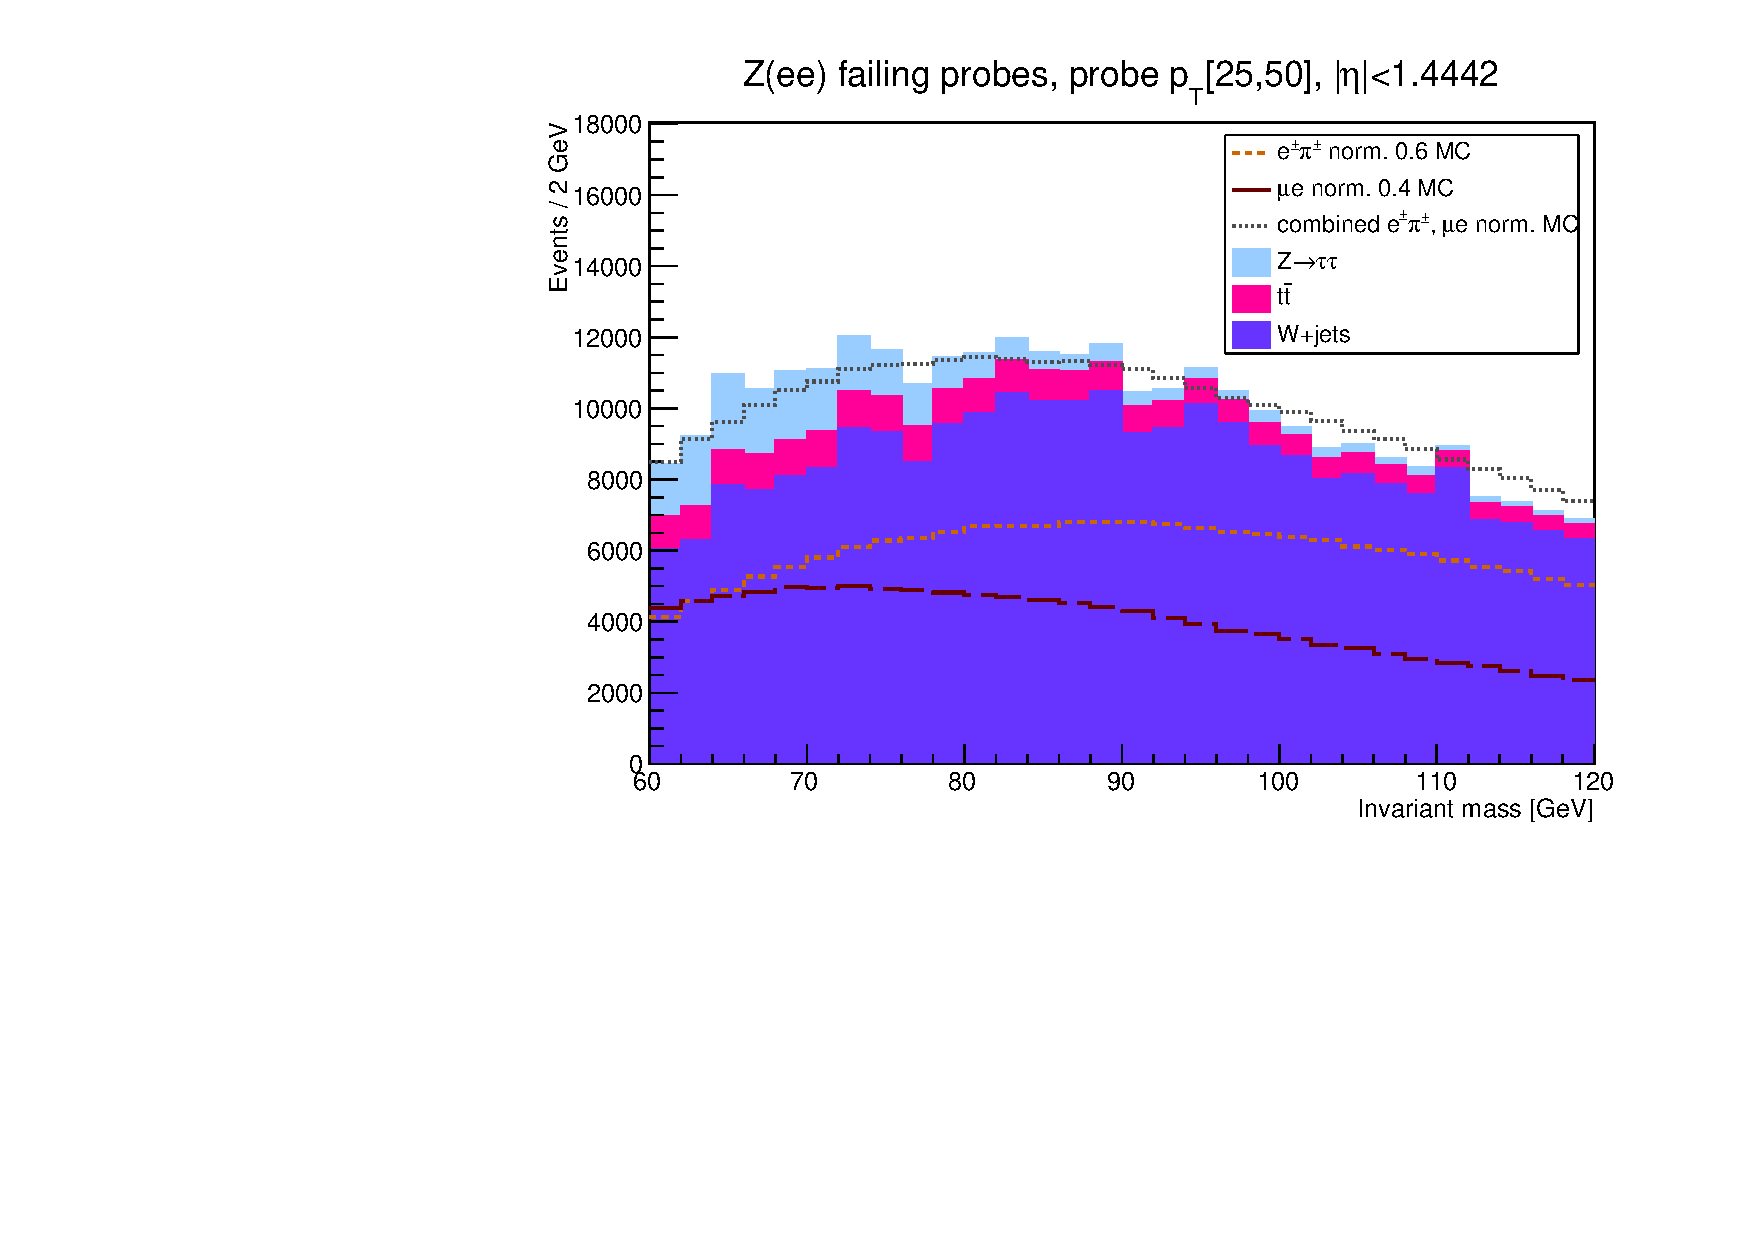
\includegraphics[width=0.75\textwidth]{figures/ZeeEPiEMu.pdf}
	\caption{Simulation of the true background shape, compared with the shapes of the \ensuremath{\ell^{\pm}\pi^{\pm}} selection, the \ensuremath{e\mu} selection, and a linear combination of the two.
    The background is normalized to the integrated luminosity of the 2016 dataset.}
	\label{fig:ZeeEPiEMu}
\end{figure}
\section{Fitting techniques}
\label{sec:tnpfits}
The data efficiency is determined by performing a combined signal plus background fit to each of the
passing and failing categories, in each of the bins of kinematic phase space. 
The efficiency extraction fit provides the number of signal Z events in the passing and failing categories 
by measuring the relative contribution of signal and background.
The nominal values for the signal and background yields in data are fit using a signal hypothesis
of truth-matched Drell-Yan Monte Carlo templates (as described in Section~\ref{sec:tnpsel}),
convoluted with a Gaussian resolution function which allows for widening and shifting of the
simulated peak position. The background hypothesis is a fixed shape derived from data, as
described in Section~\ref{sec:tnpcontrol}.
In the dielectron fits, the relative contribution of \ensuremath{e^{\pm}\pi^{\pm}} versus 
{\ensuremath{e\mu} data is a free parameter in the fit.

The binning choice for the probe leptons is the following:
\begin{itemize}
\item Probe electron $\pt$: $\{$10, 15, 20, 25, 30, 35, 40, 42, 44, 46, 48, 50, 55, 60, 70, 100$\}$ $\GeV$;
\item Probe electron $\eta$: $\{$-2.5, -2.4, -2.3, -2.2, -2.1, -2.0, -1.8, -1.566, -1.4442, -1.2, -1, -0.8, -0.6, -0.4, -0.2, 0, 0.2, 0.4, 0.6, 0.8, 1, 1.2, 1.4442, 1.566, 1.8, 2.0, 2.1, 2.2, 2.3, 2.4, 2.5$\}$;
\item Probe muon $\pt$: $\{$10, 15, 20, 25, 30, 35, 40, 45, 50, 55, 60, 120$\}$ $\GeV$;
\item Probe muon $\eta$: $\{$-2.4, -2.1, -1.6, -1.2, -0.9, -0.3, -0.2, 0.2, 0.3, 0.9, 1.2, 1.6, 2.1, 2.4$\}$;
\end{itemize}

Representing the phase space bin and the pass/fail category with the index $i$,
the number of signal events $N_{sig}^{i}$ (and associated statistical uncertainty) in this bin
is calculated as the total number of data events $N_{total}^{i}$ (Poisson distributed),
minus the estimated background yield $N_{bkg}^{i}$
(with statistical uncertainty from the negative likelihood minimization procedure).
Then, in each phase space bin, the efficiency is determined as
\begin{align*}
  \varepsilon = \frac{N_{sig}^{pass}}{N_{sig}^{pass}+N_{sig}^{fail}}
\end{align*}
and the statistical errors are propagated conservatively assuming zero, not negative
correlation between the passing and failing signal yields.

Examples of the nominal efficiency extraction fits for dimuons are shown in Figures~\ref{fig:ZmmNominalFits1} and~\ref{fig:ZmmNominalFits2}.
Similar examples for dielectrons are shown in Figures~\ref{fig:ZeeNominalFits1} and~\ref{fig:ZeeNominalFits2}.
In order to assess the goodness-of-fit, we compute a modified $\chi^2$ test which accounts for
statistical uncertainties in the data as well as the MC signal template, as shown in the plots.

The MC efficiency is determined by counting the normalized yields of the passing and failing templates described above.
\begin{figure}
\centering
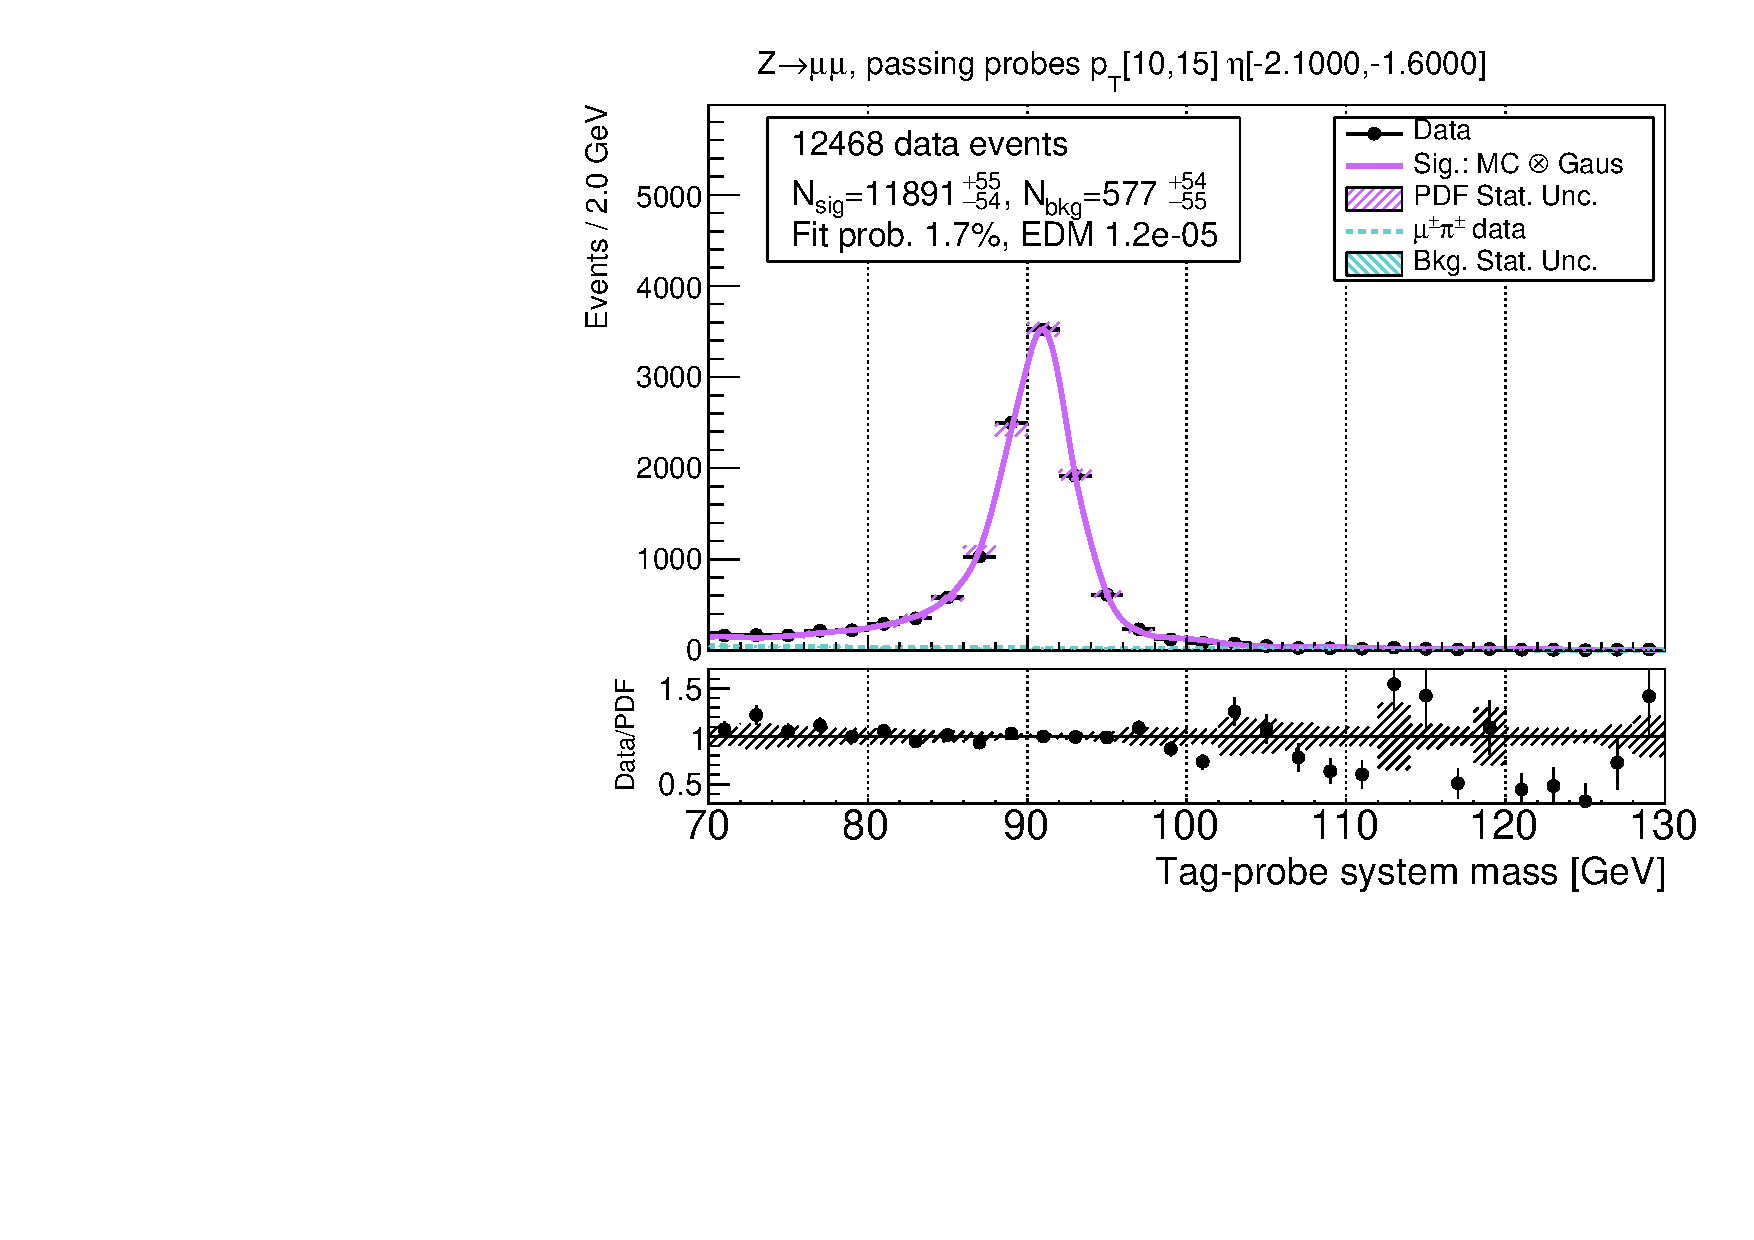
\includegraphics[width=0.49\textwidth]{figures/Zmm_RecoTemplate_BkgLPi_pass_ptBin0_etaBin1.pdf}
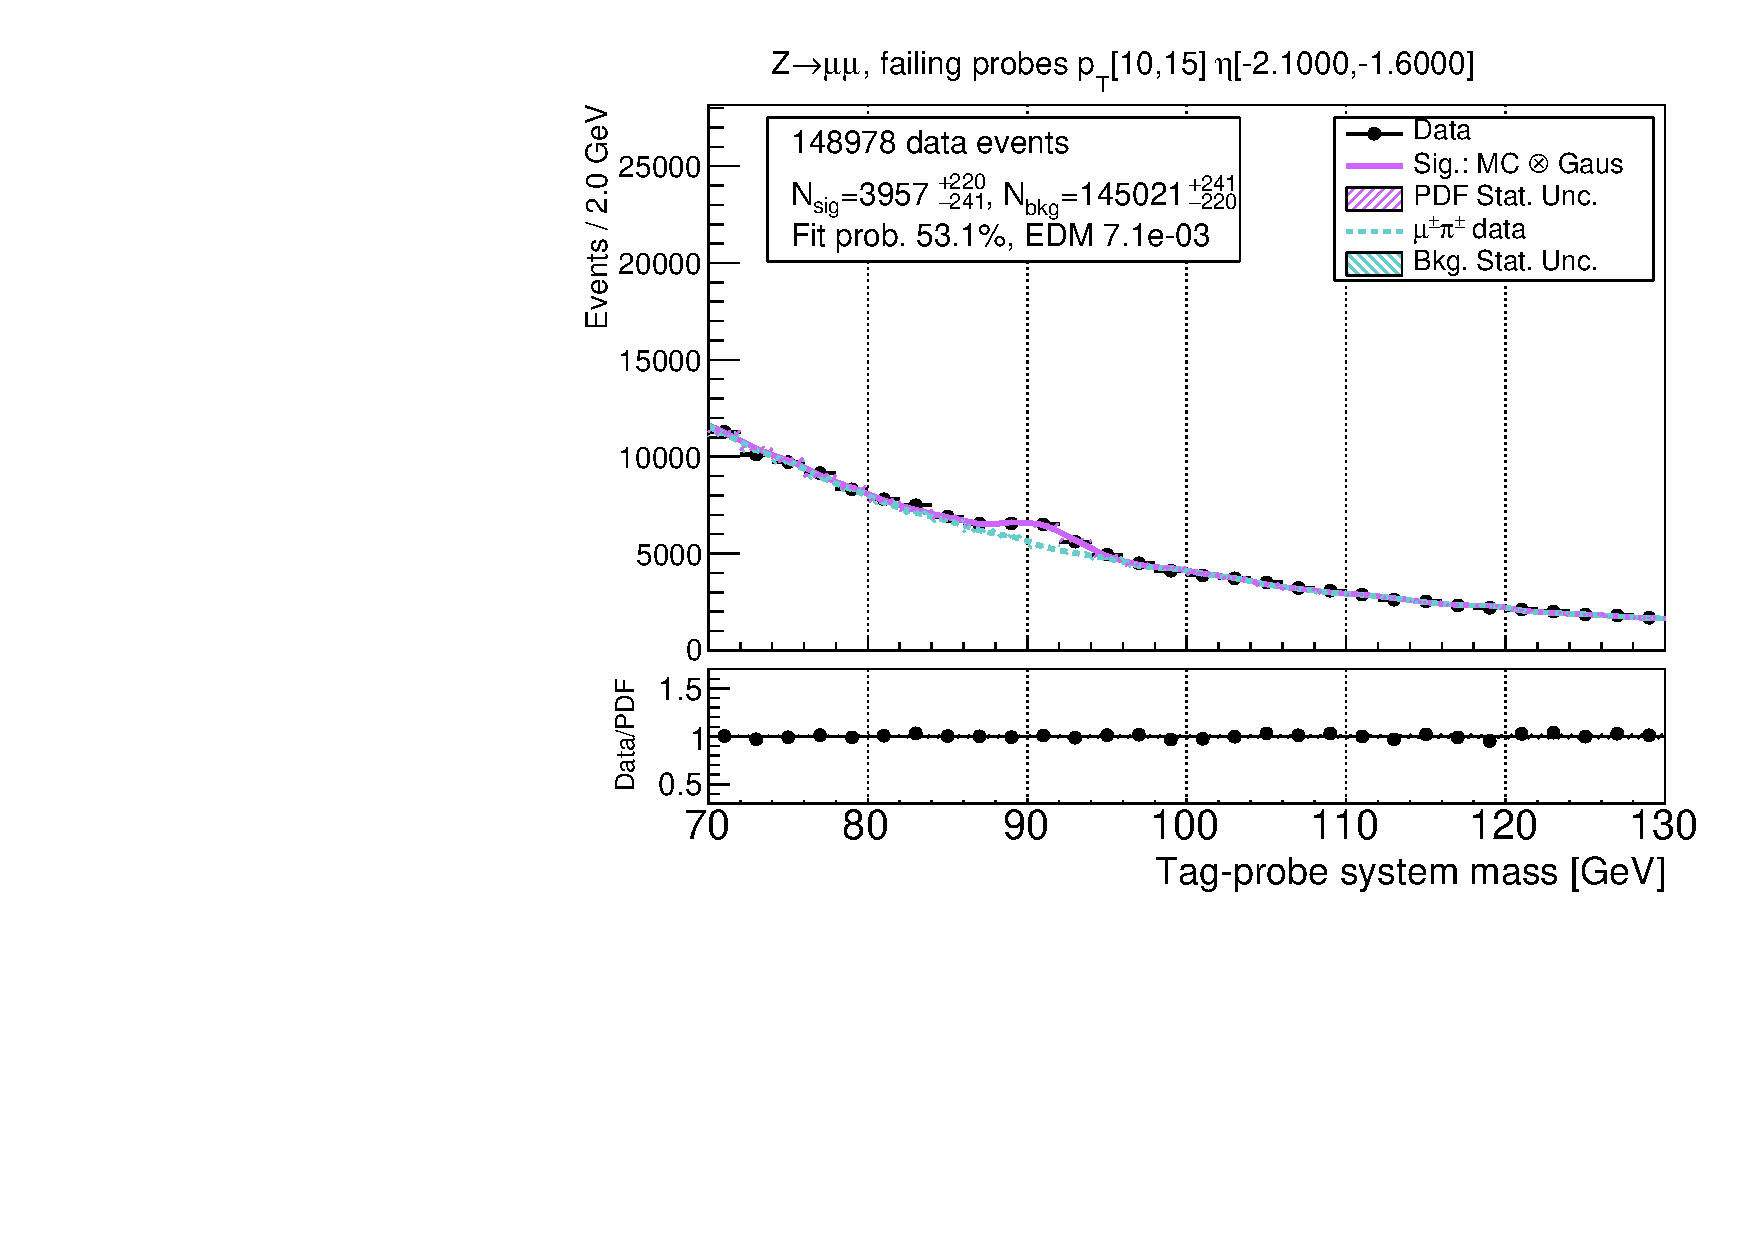
\includegraphics[width=0.49\textwidth]{figures/Zmm_RecoTemplate_BkgLPi_fail_ptBin0_etaBin1.pdf}
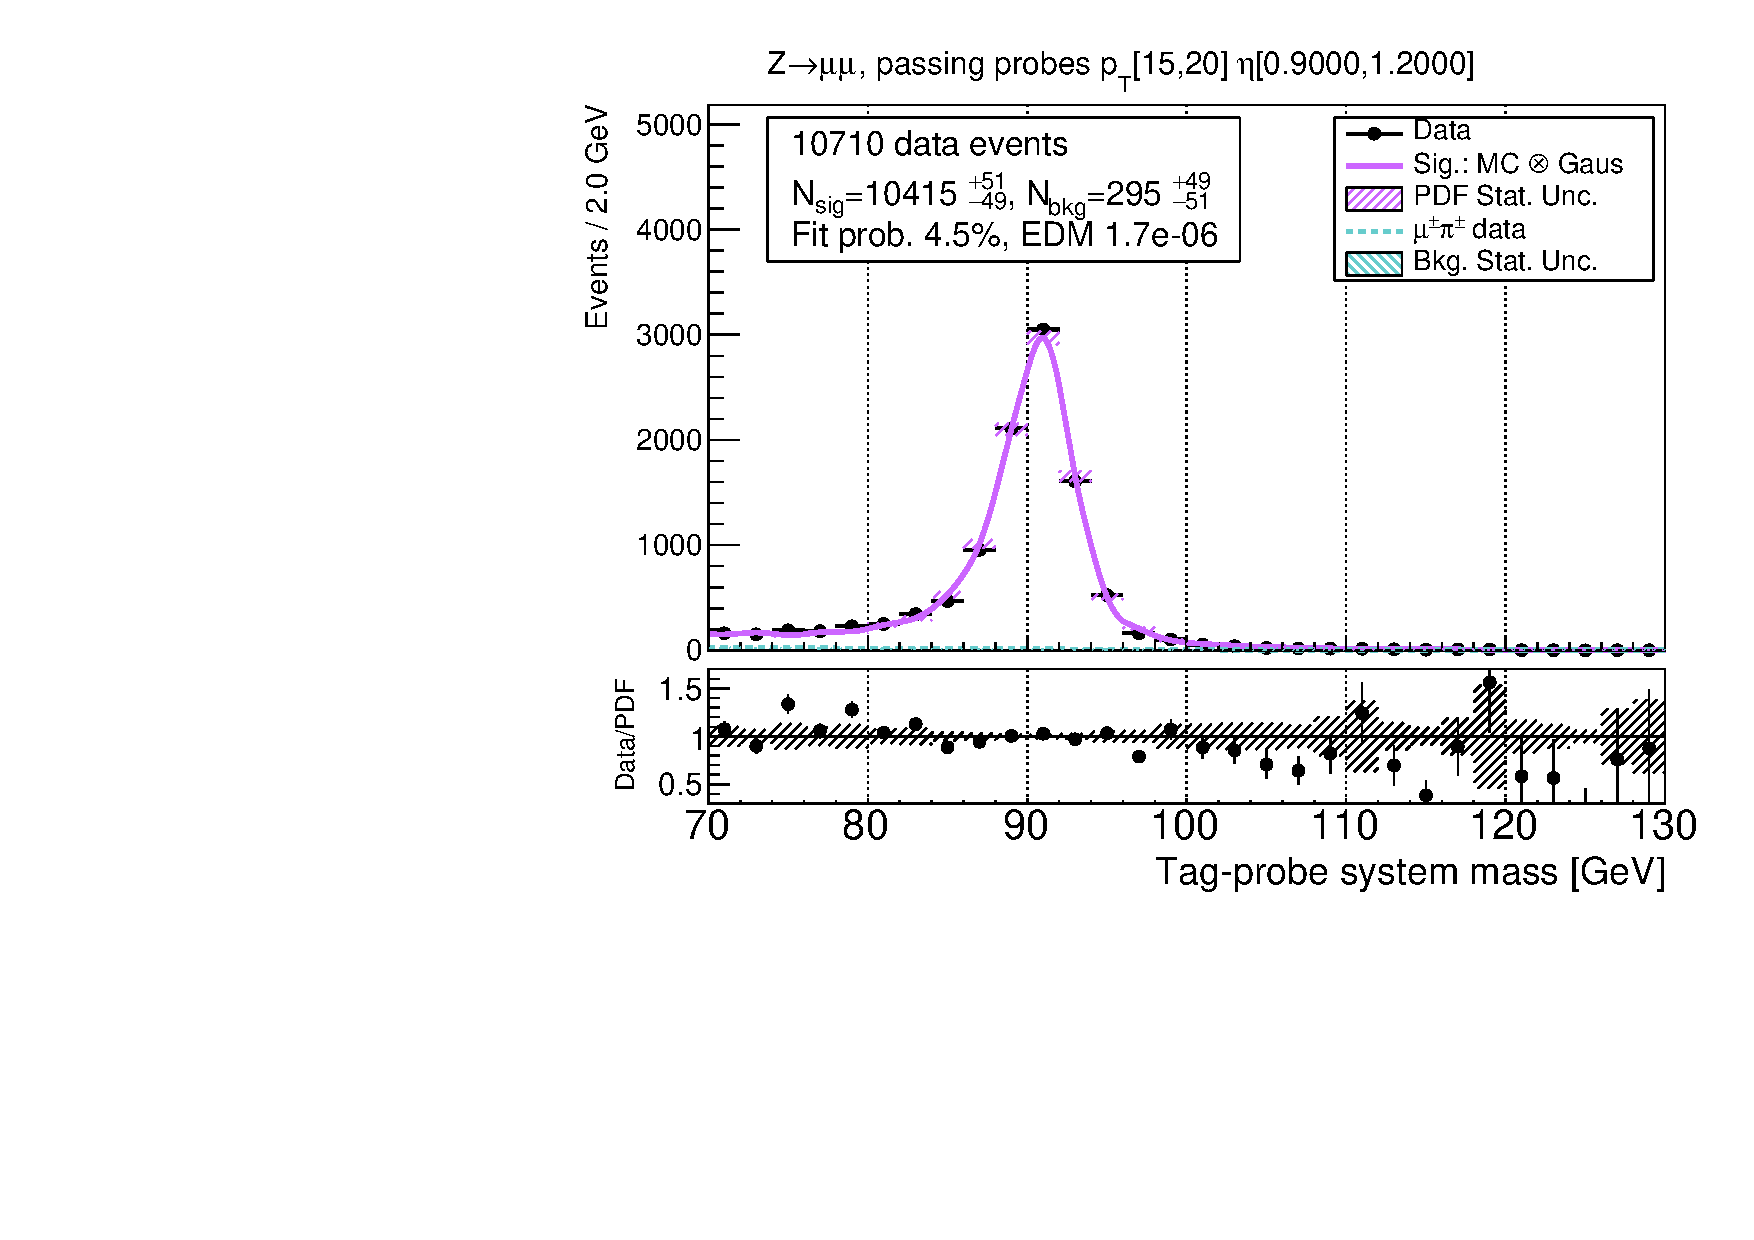
\includegraphics[width=0.49\textwidth]{figures/Zmm_RecoTemplate_BkgLPi_pass_ptBin1_etaBin9.pdf}
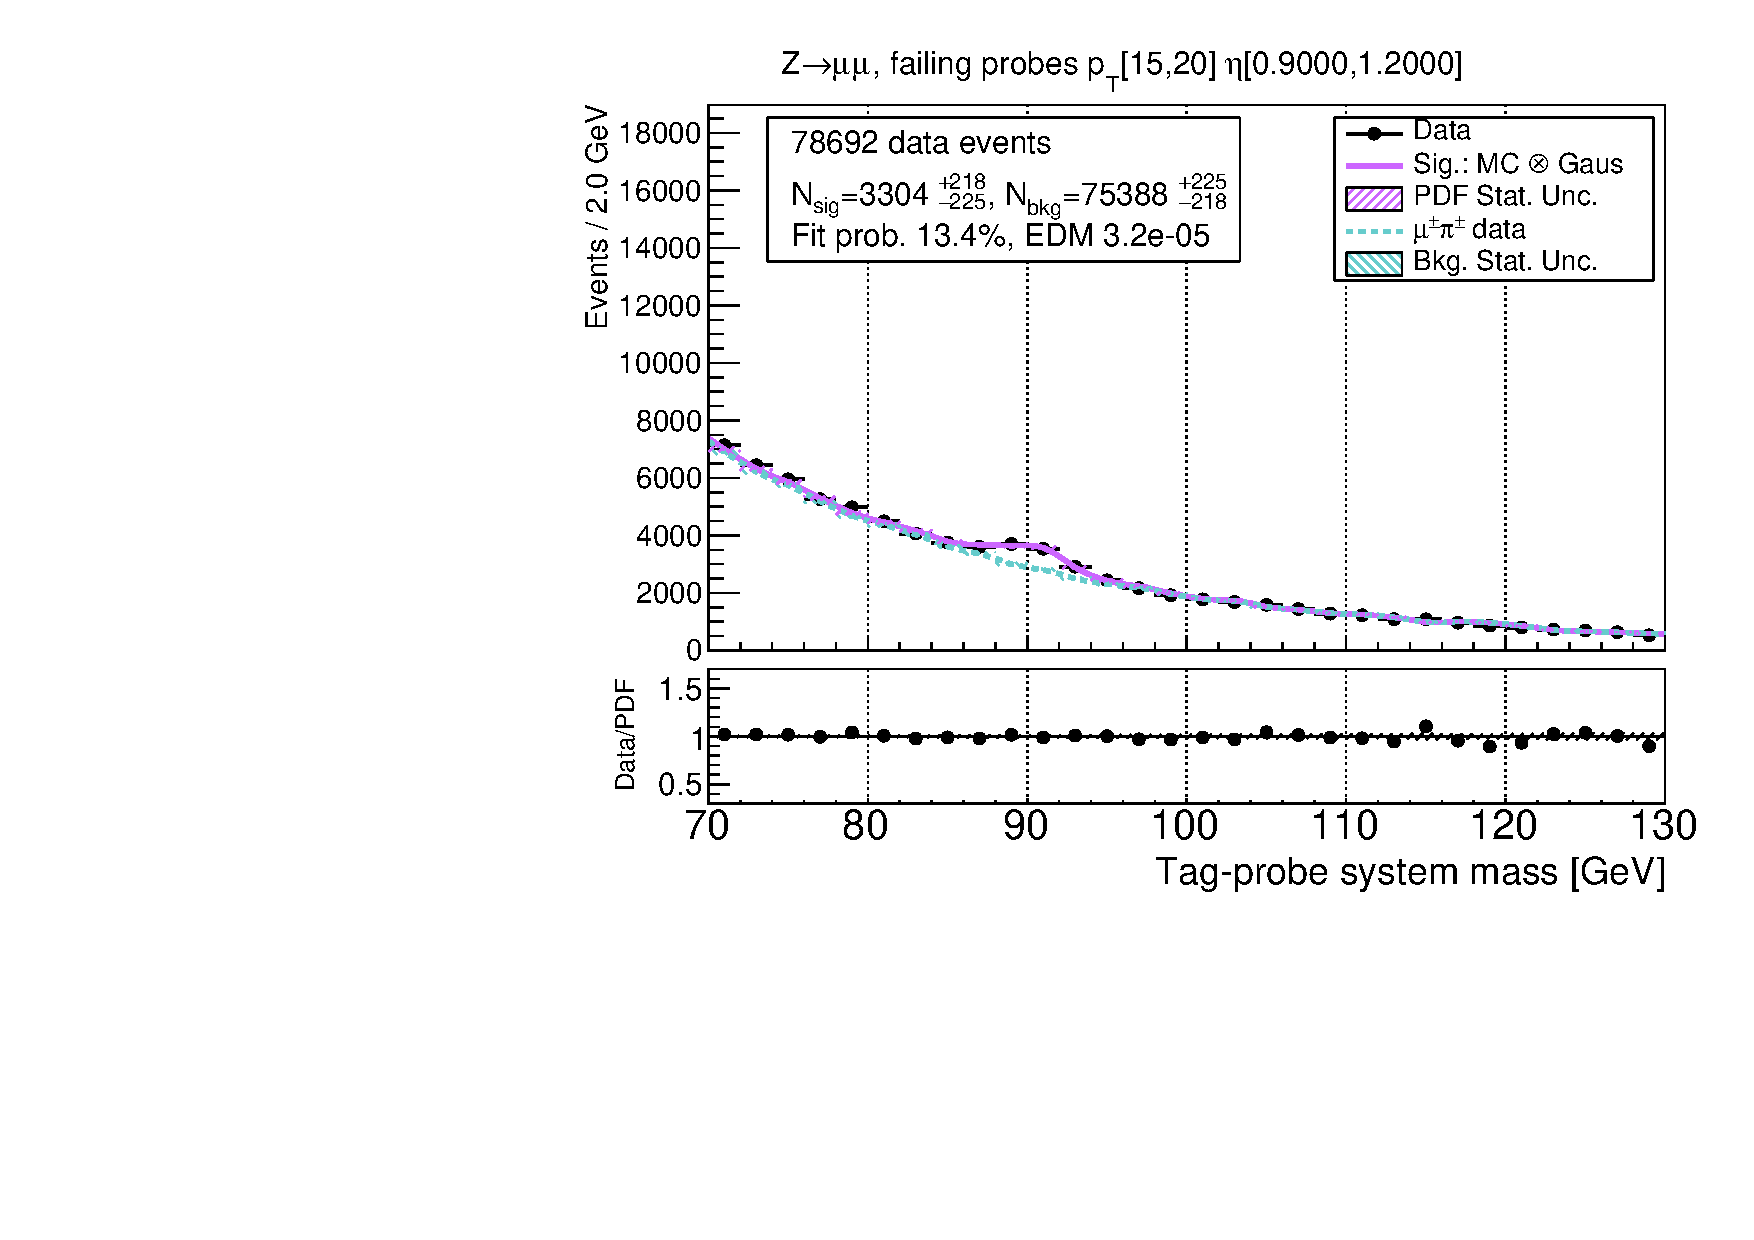
\includegraphics[width=0.49\textwidth]{figures/Zmm_RecoTemplate_BkgLPi_fail_ptBin1_etaBin9.pdf}
\caption{Efficiency extraction fits for the Medium muon working point using the data-driven background shape, at low muon transverse momentum.}
\label{fig:ZmmNominalFits1}
\end{figure}
\begin{figure}
\centering
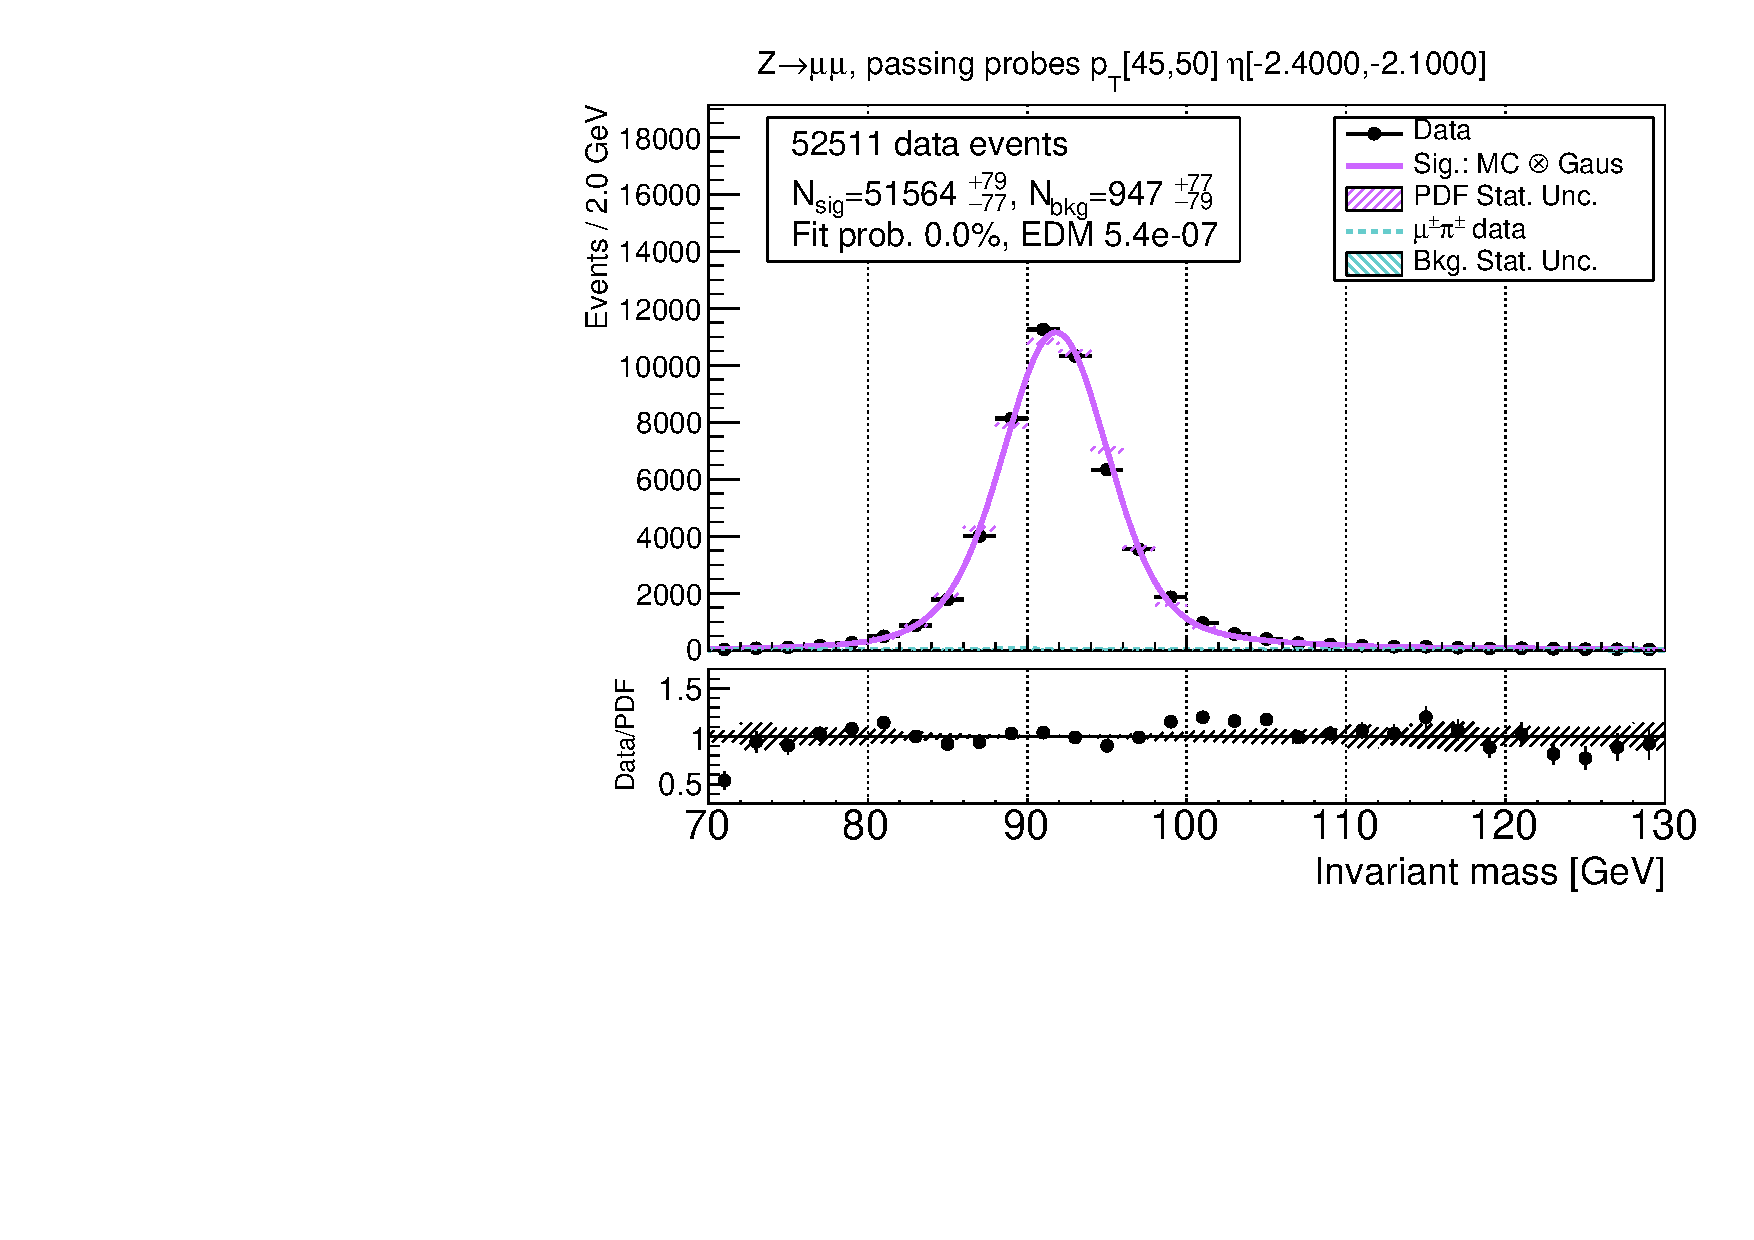
\includegraphics[width=0.49\textwidth]{figures/Zmm_RecoTemplate_BkgLPi_pass_ptBin7_etaBin0.pdf}
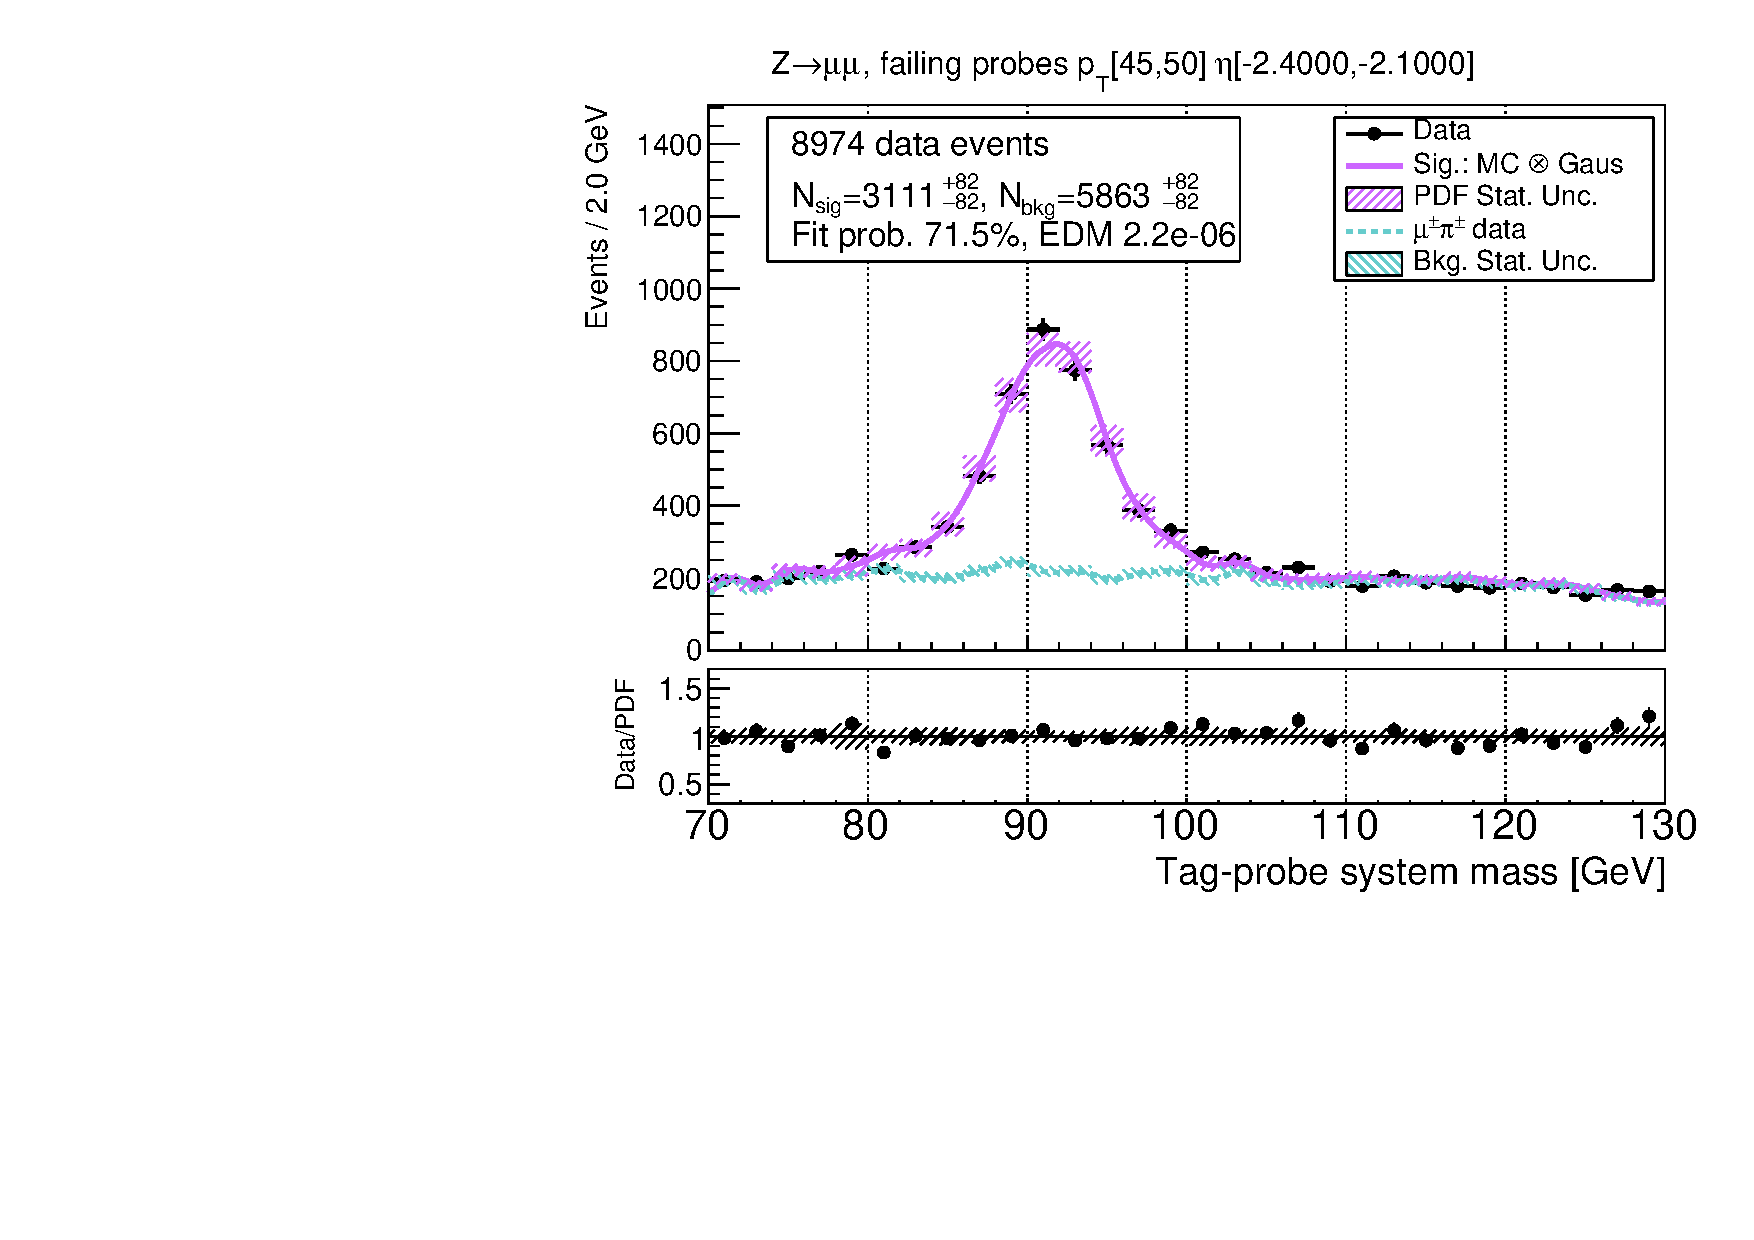
\includegraphics[width=0.49\textwidth]{figures/Zmm_RecoTemplate_BkgLPi_fail_ptBin7_etaBin0.pdf}
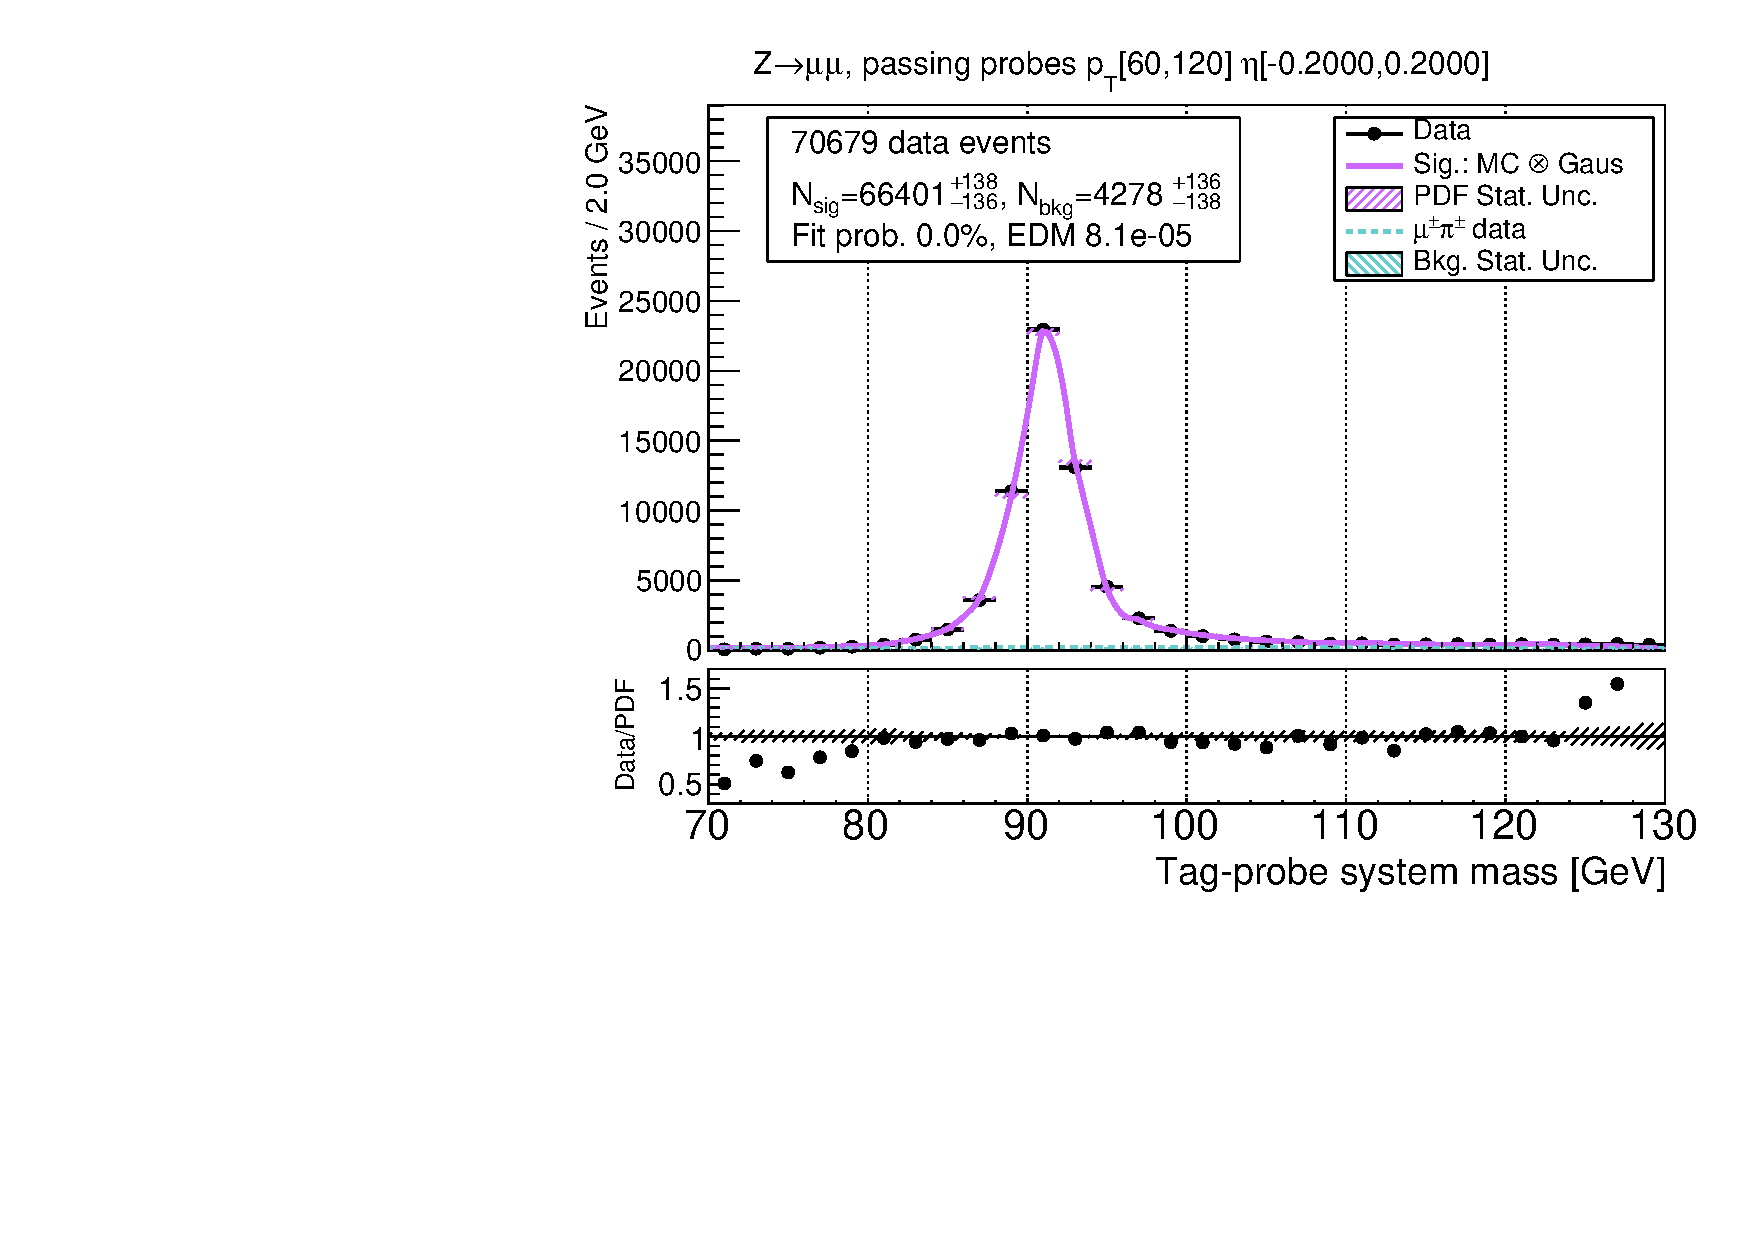
\includegraphics[width=0.49\textwidth]{figures/Zmm_RecoTemplate_BkgLPi_pass_ptBin10_etaBin6.pdf}
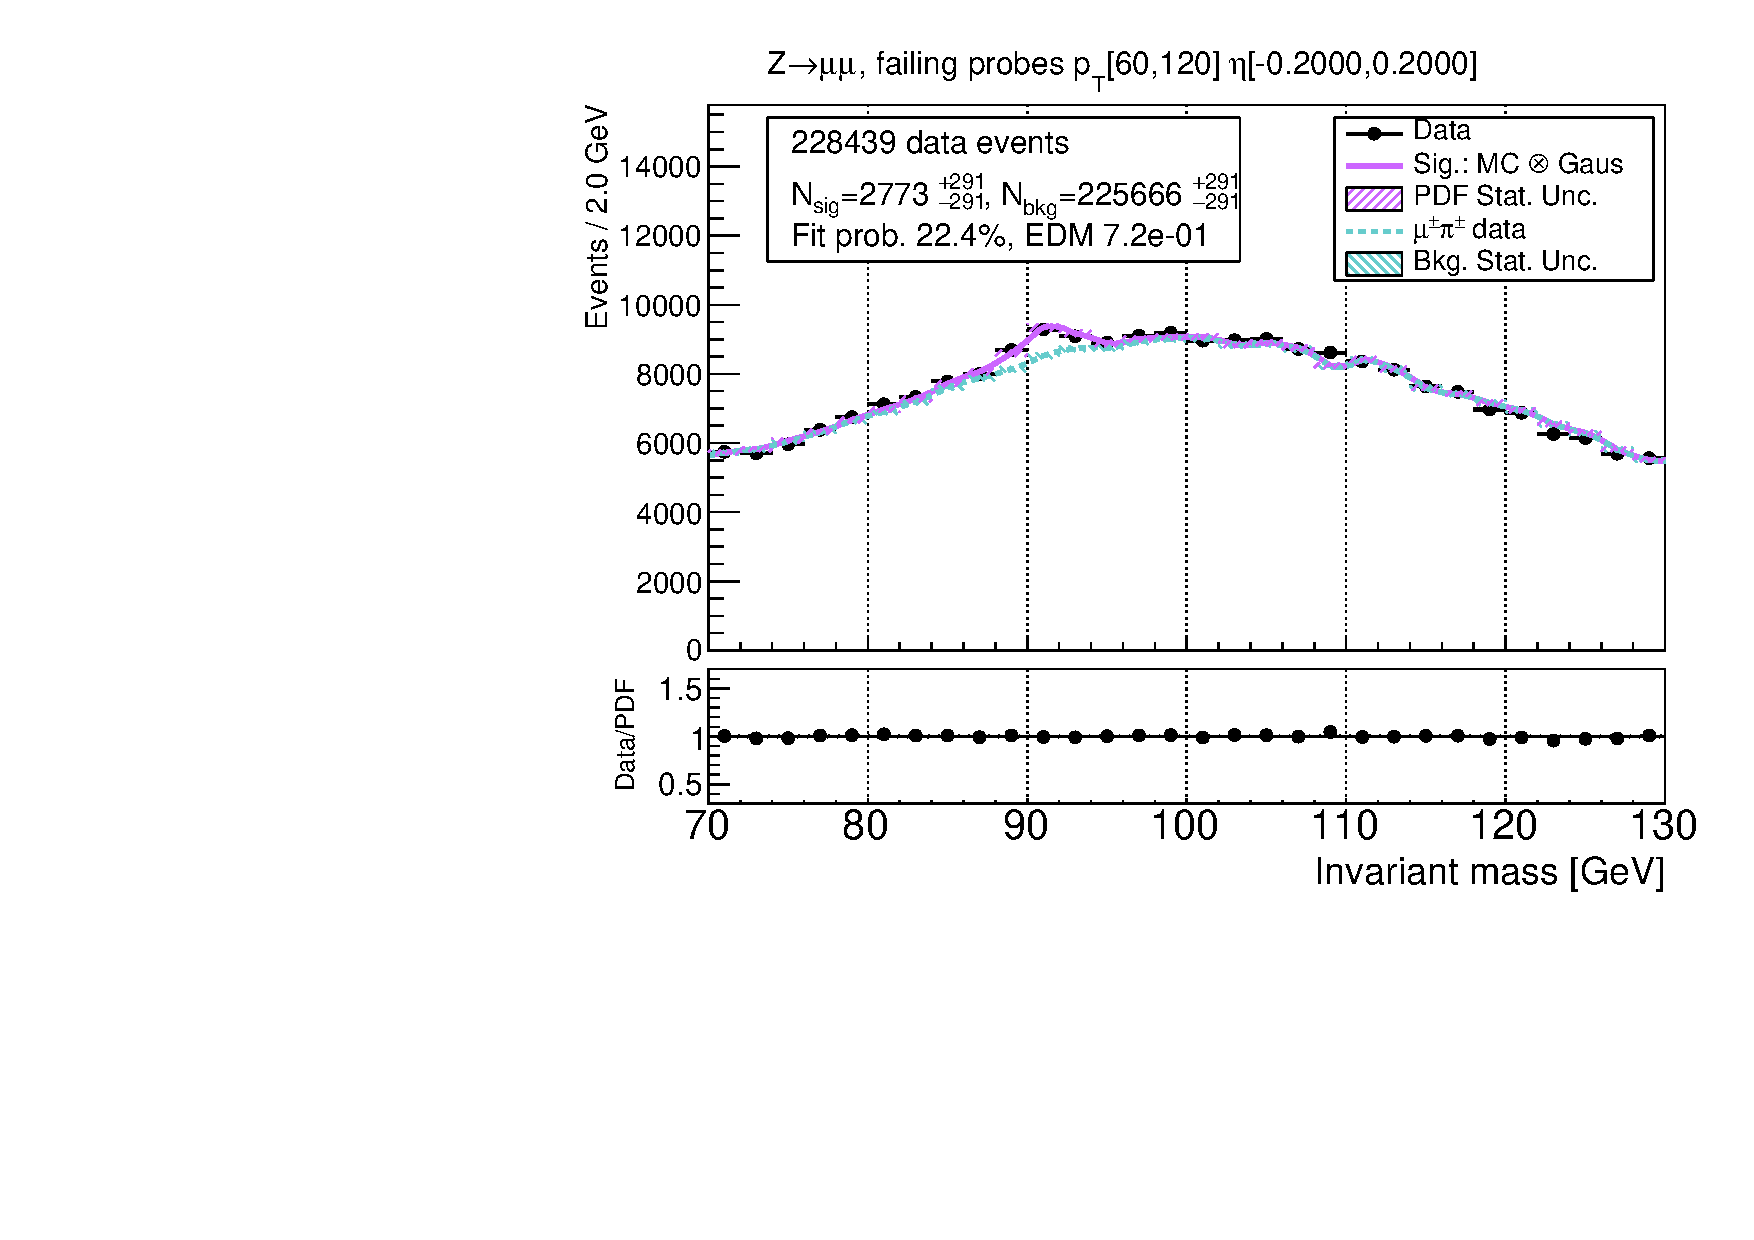
\includegraphics[width=0.49\textwidth]{figures/Zmm_RecoTemplate_BkgLPi_fail_ptBin10_etaBin6.pdf}
\caption{Efficiency extraction fits for the Medium muon working point using the data-driven background shape, at higher values of muon transverse momentum.}
\label{fig:ZmmNominalFits2}
\end{figure}

\begin{figure}
\centering
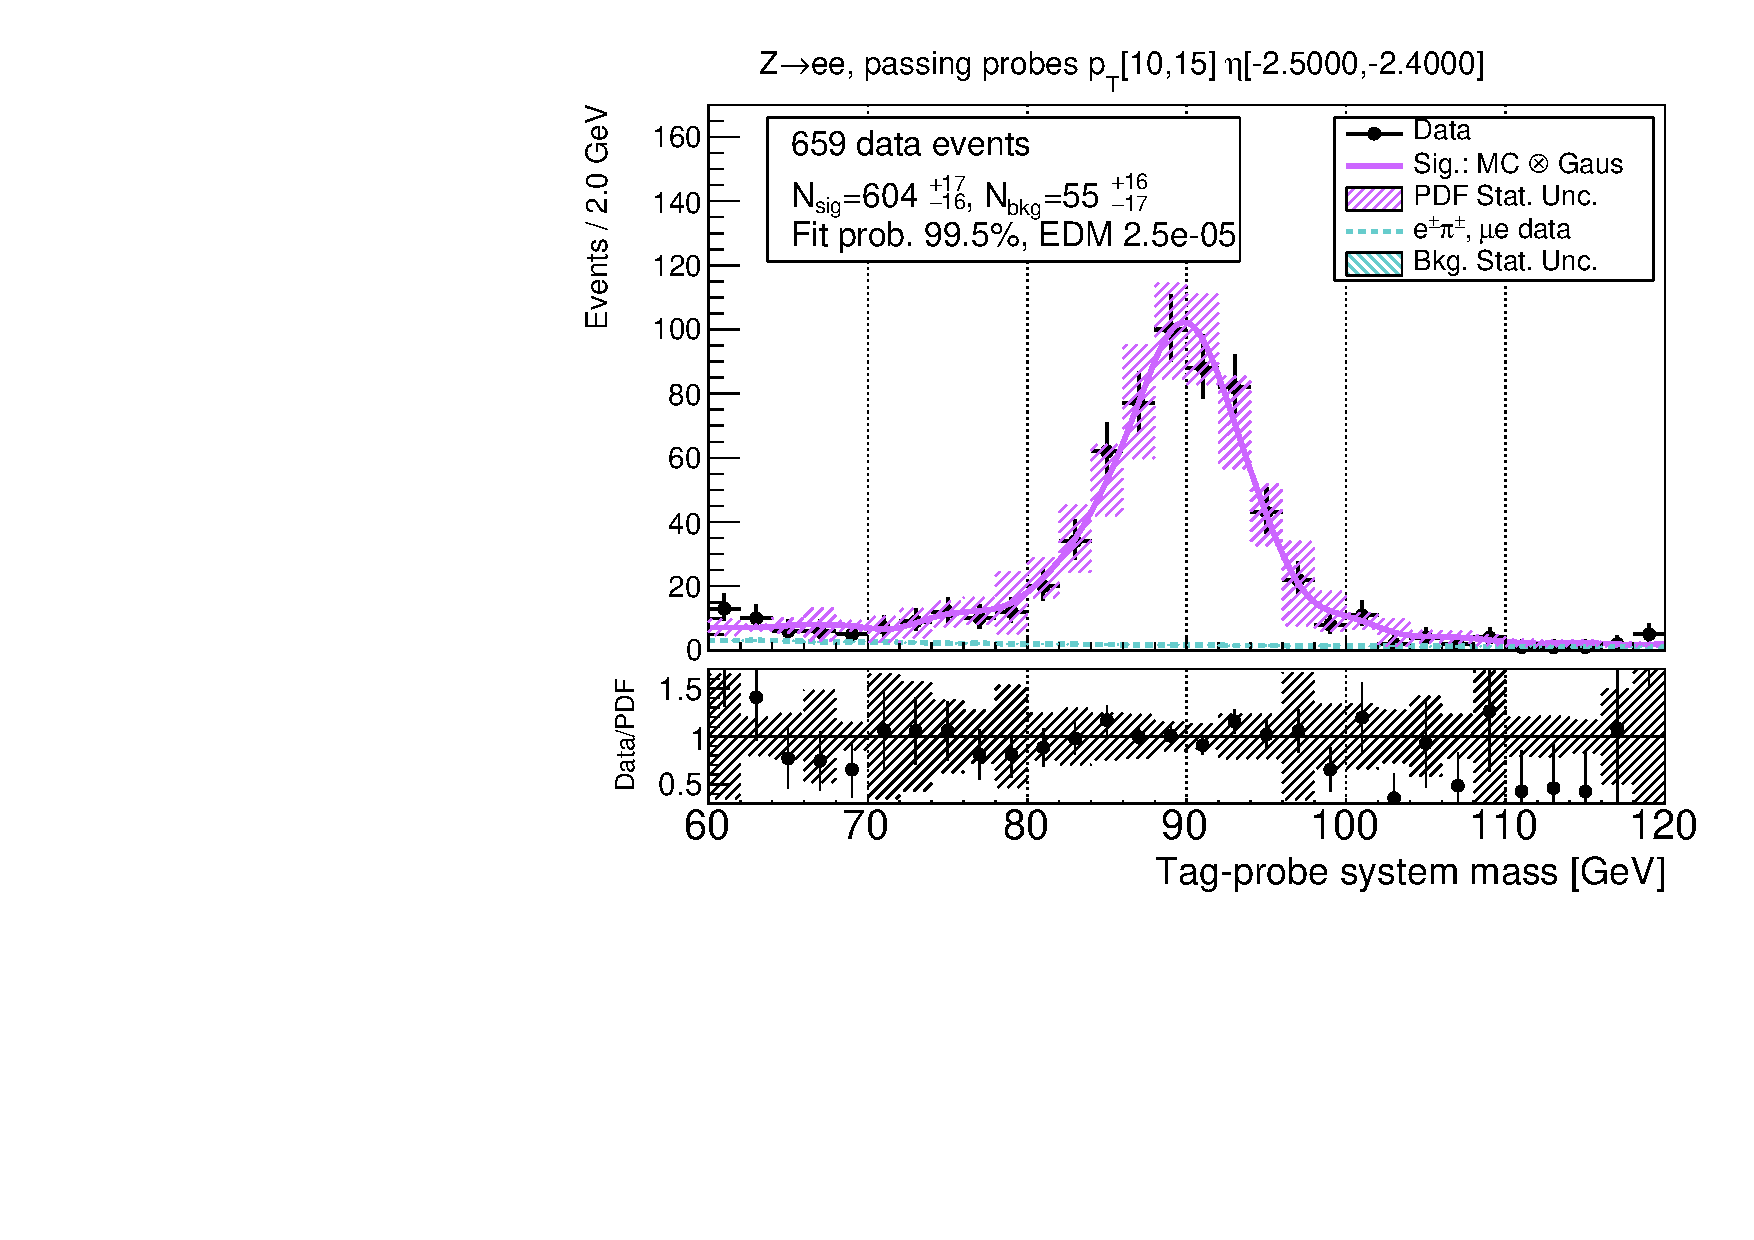
\includegraphics[width=0.49\textwidth]{figures/Zee_RecoTemplate_BkgLPiEMu_pass_ptBin0_etaBin0.pdf}
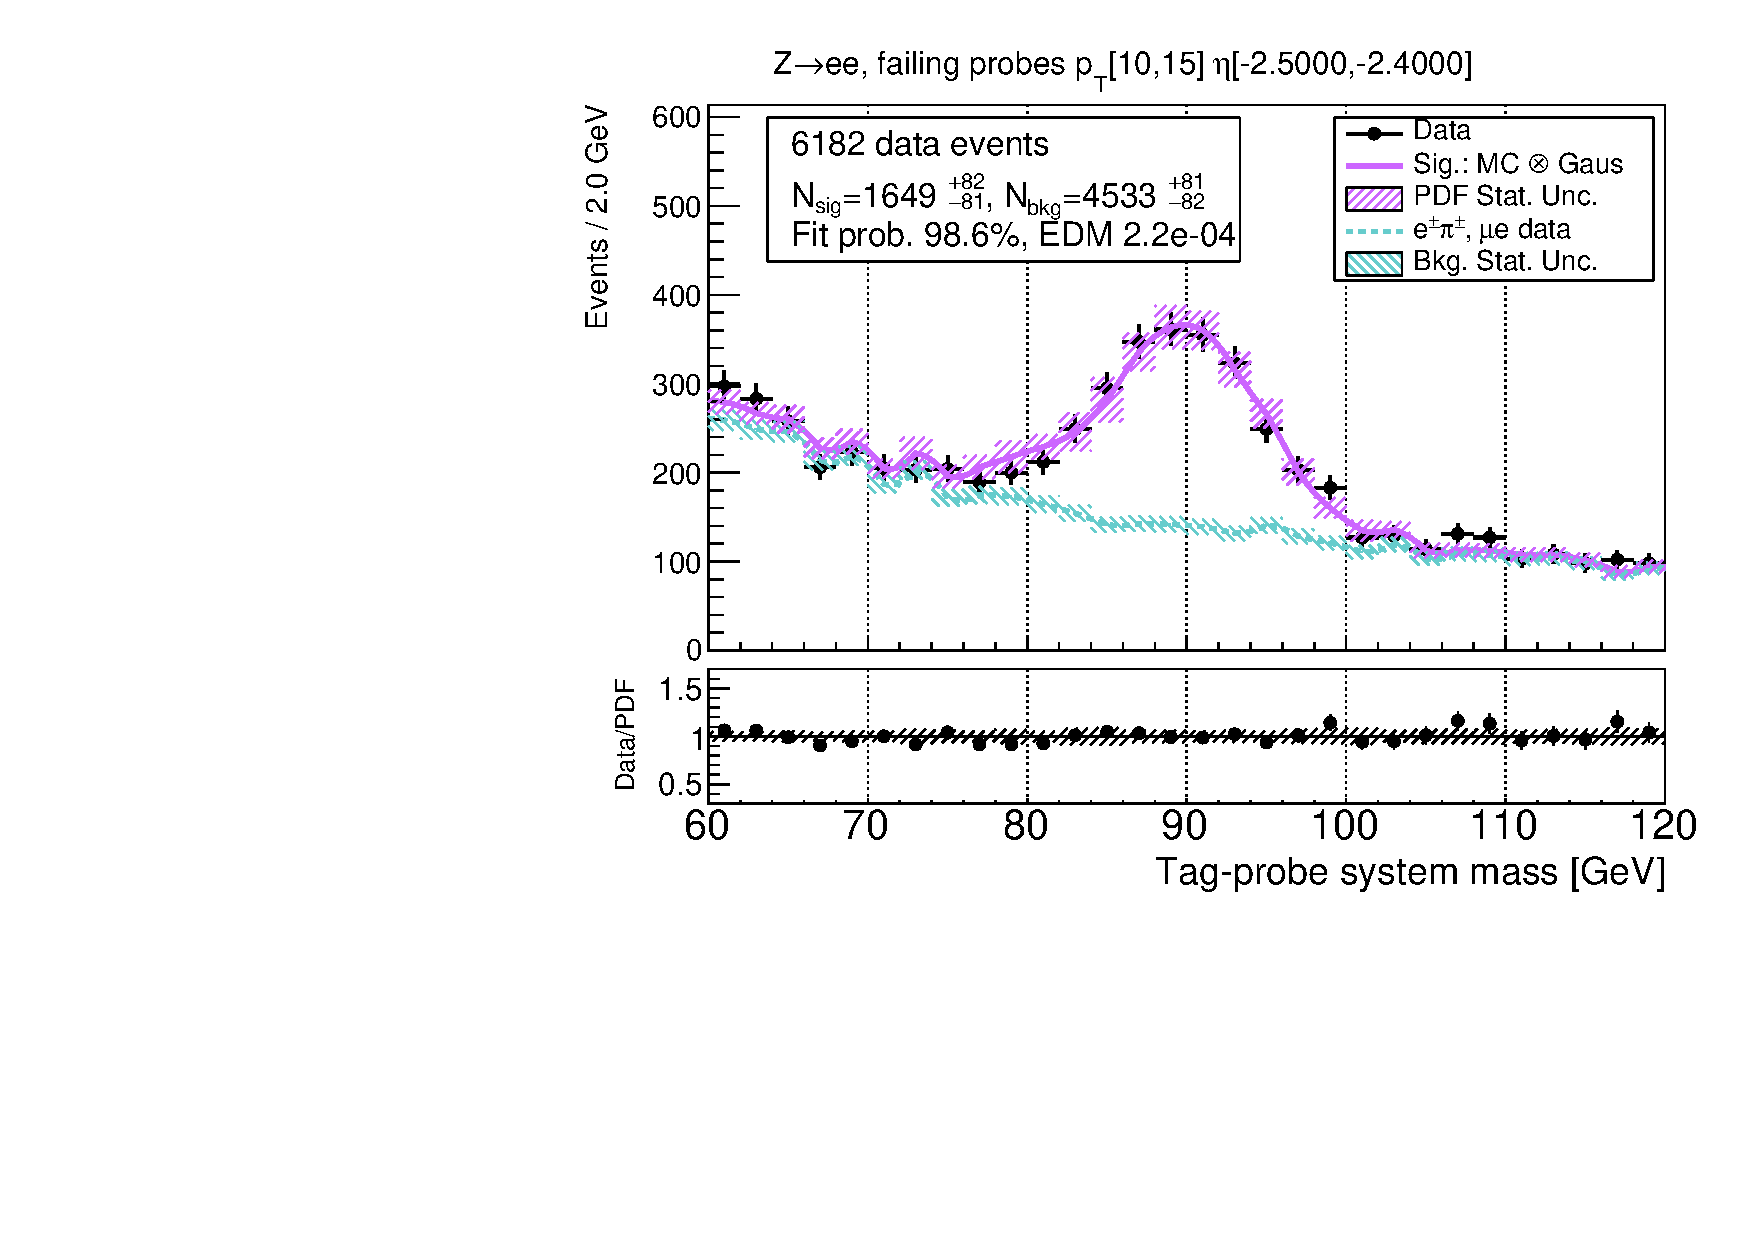
\includegraphics[width=0.49\textwidth]{figures/Zee_RecoTemplate_BkgLPiEMu_fail_ptBin0_etaBin0.pdf}
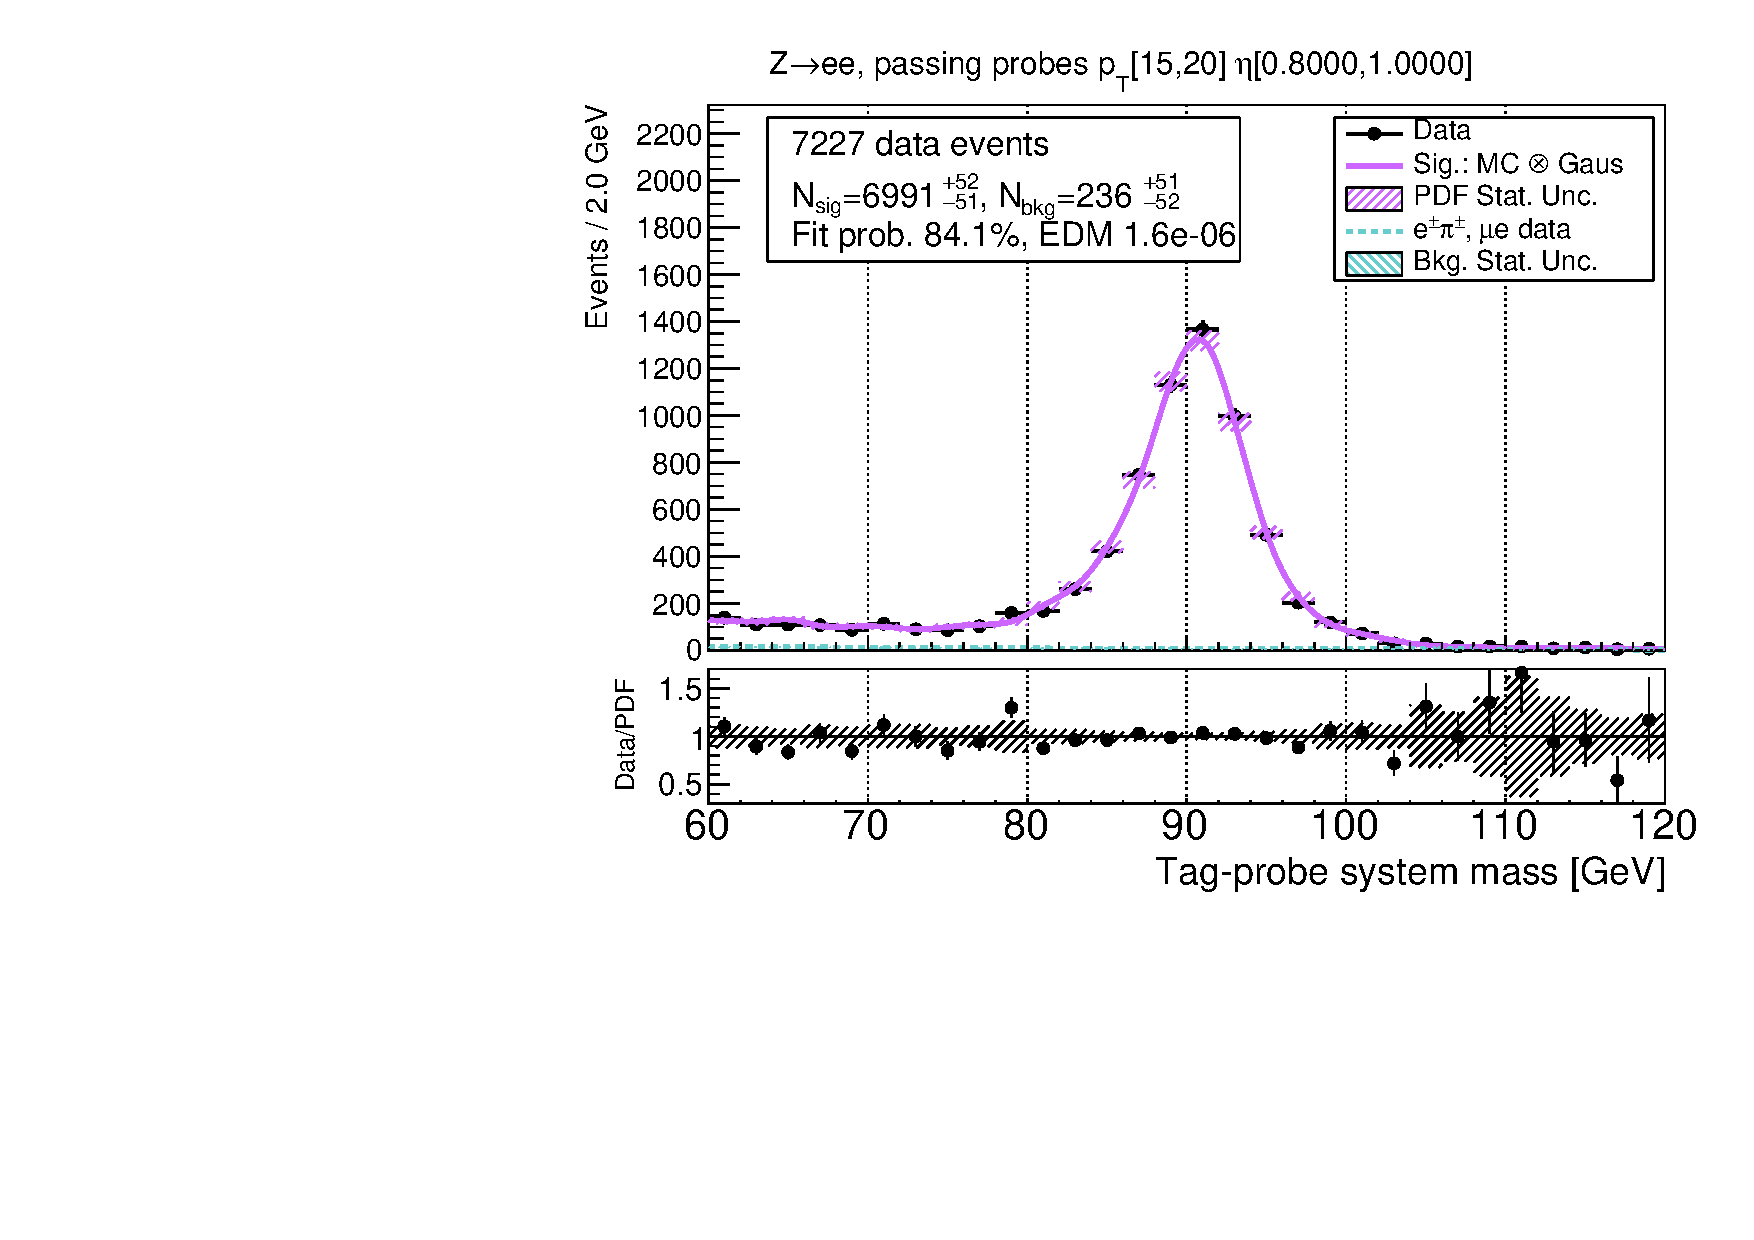
\includegraphics[width=0.49\textwidth]{figures/Zee_RecoTemplate_BkgLPiEMu_pass_ptBin1_etaBin19.pdf}
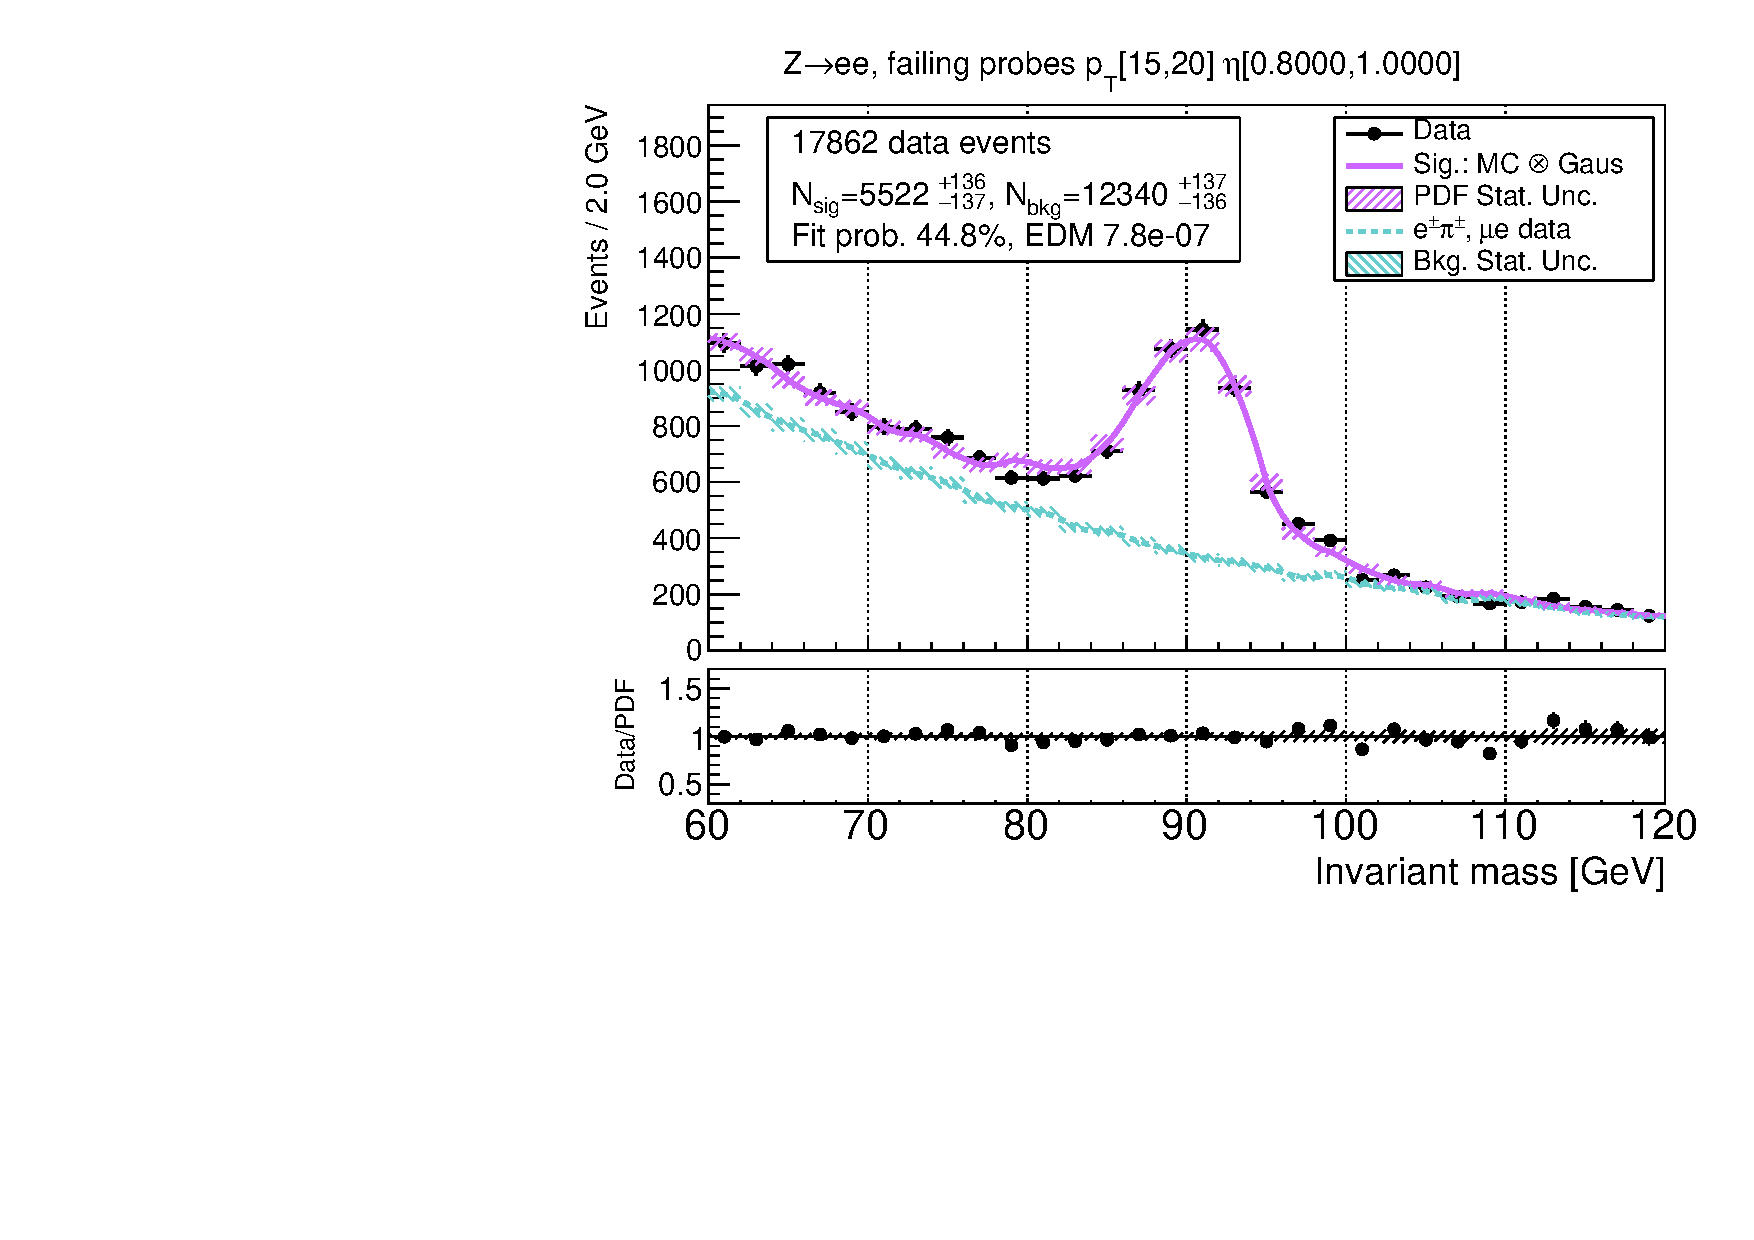
\includegraphics[width=0.49\textwidth]{figures/Zee_RecoTemplate_BkgLPiEMu_fail_ptBin1_etaBin19.pdf}
\caption{Efficiency extraction fits for the Medium electron working point using the data-driven background shape, at low electron transverse momentum.}
\label{fig:ZeeNominalFits1}
\end{figure}
\begin{figure}
\centering
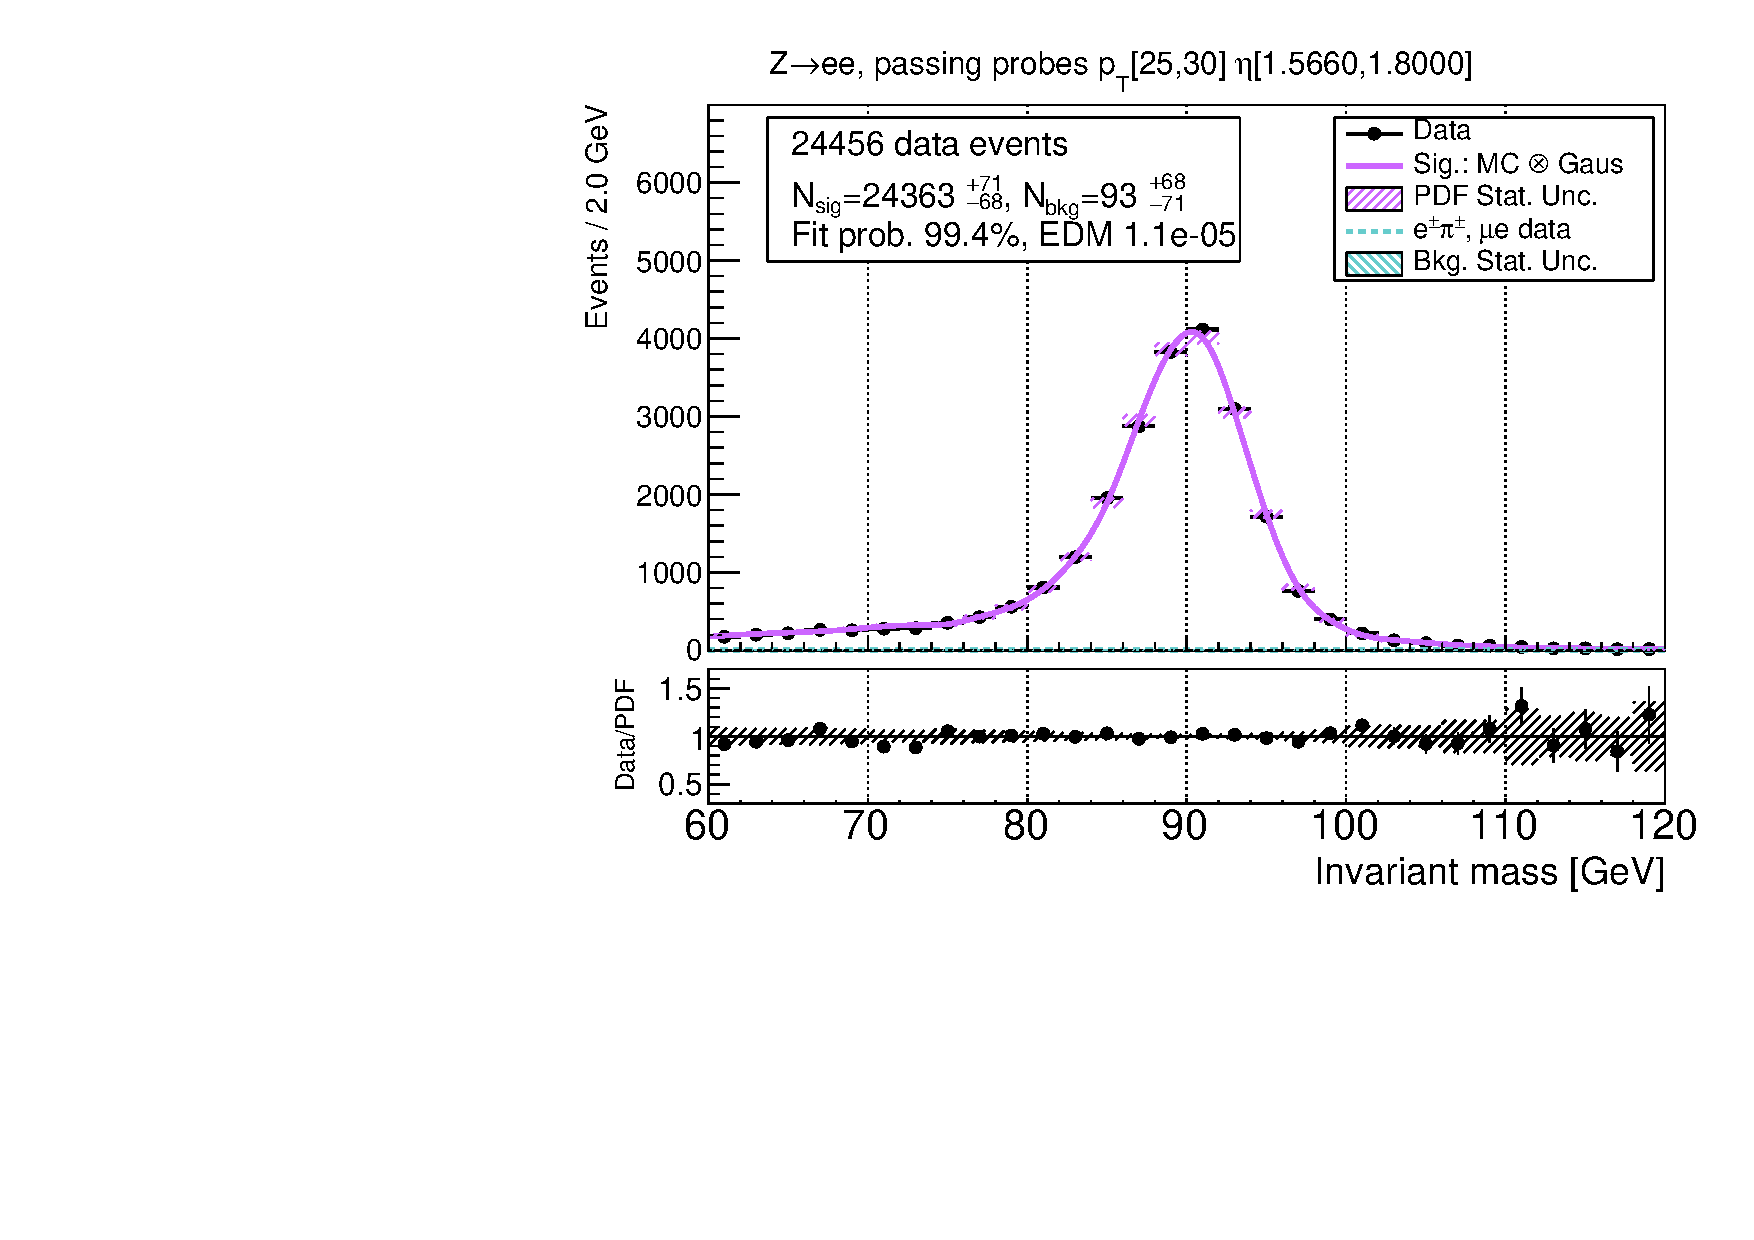
\includegraphics[width=0.49\textwidth]{figures/Zee_RecoTemplate_BkgLPiEMu_pass_ptBin3_etaBin23.pdf}
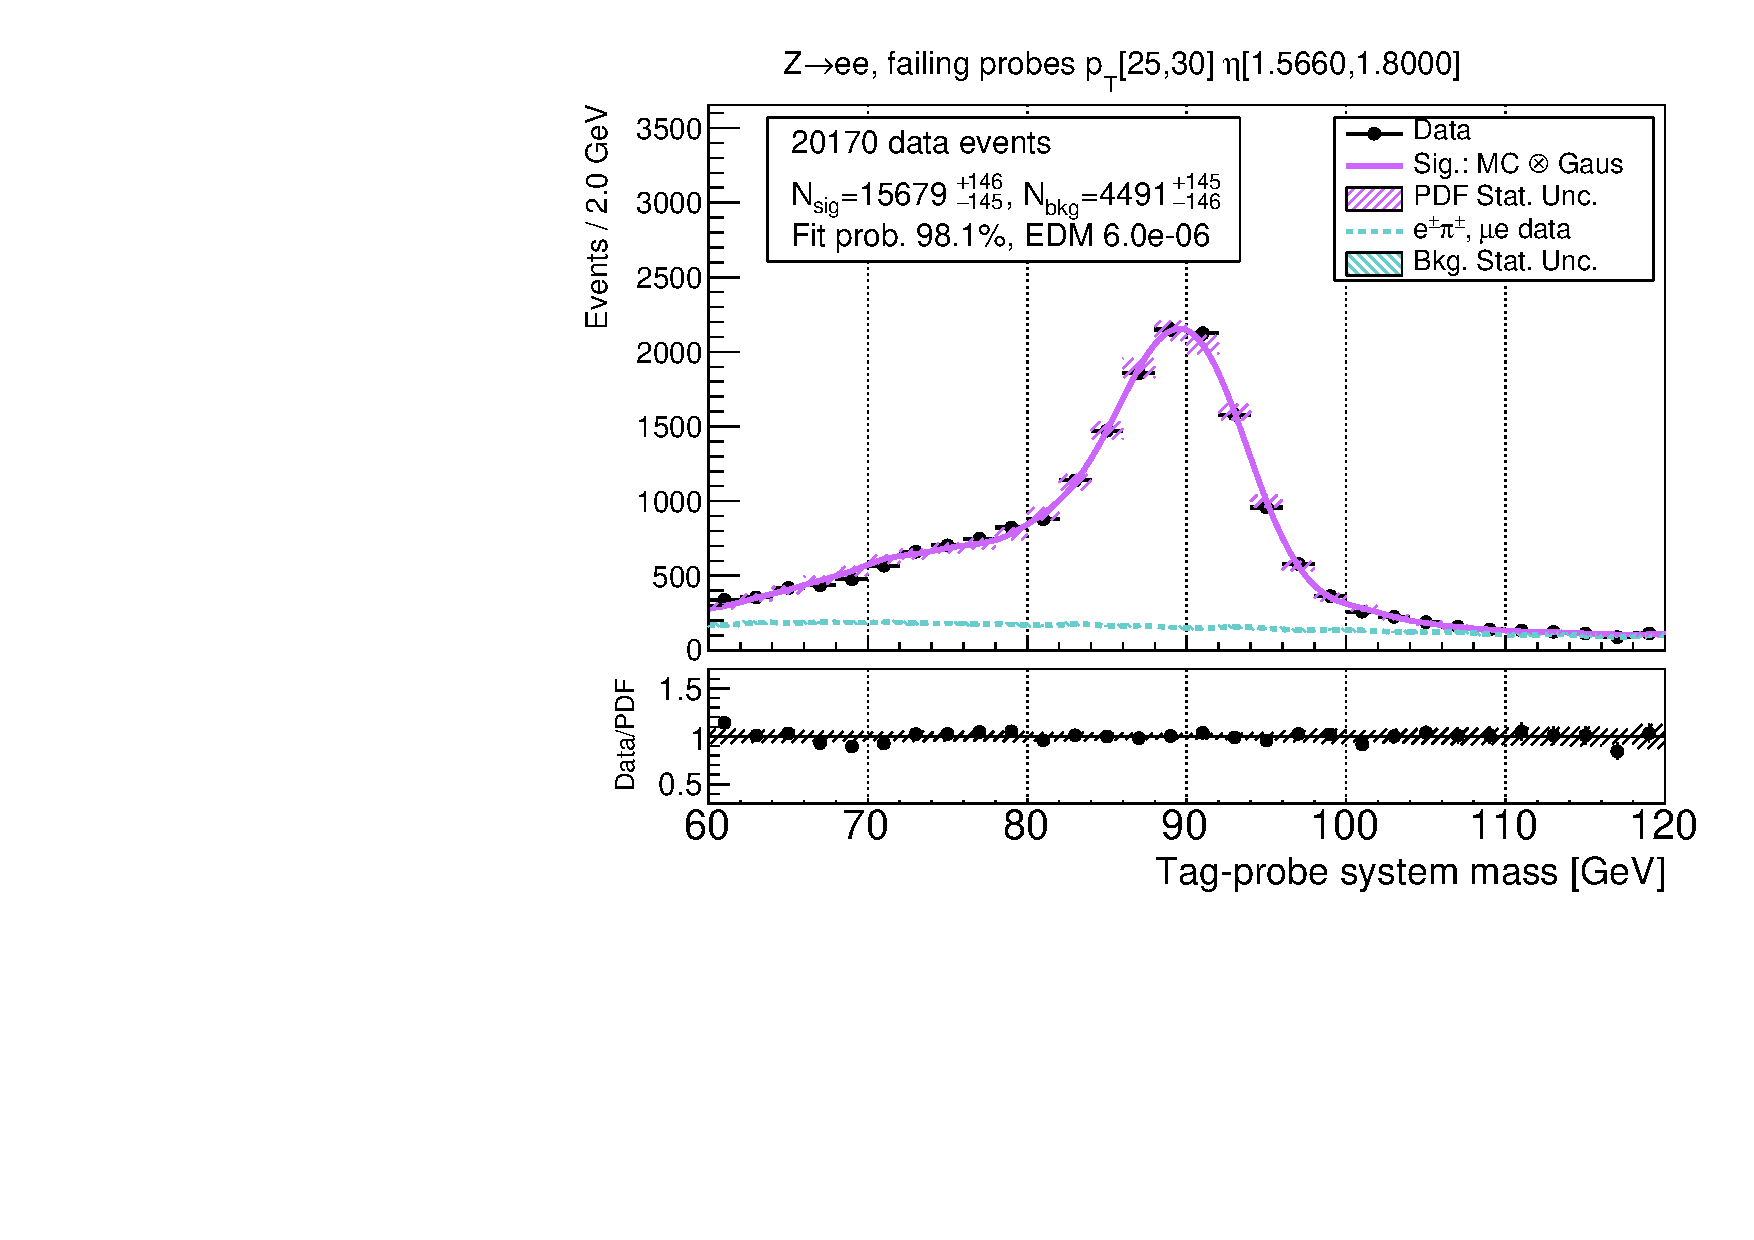
\includegraphics[width=0.49\textwidth]{figures/Zee_RecoTemplate_BkgLPiEMu_fail_ptBin3_etaBin23.pdf}
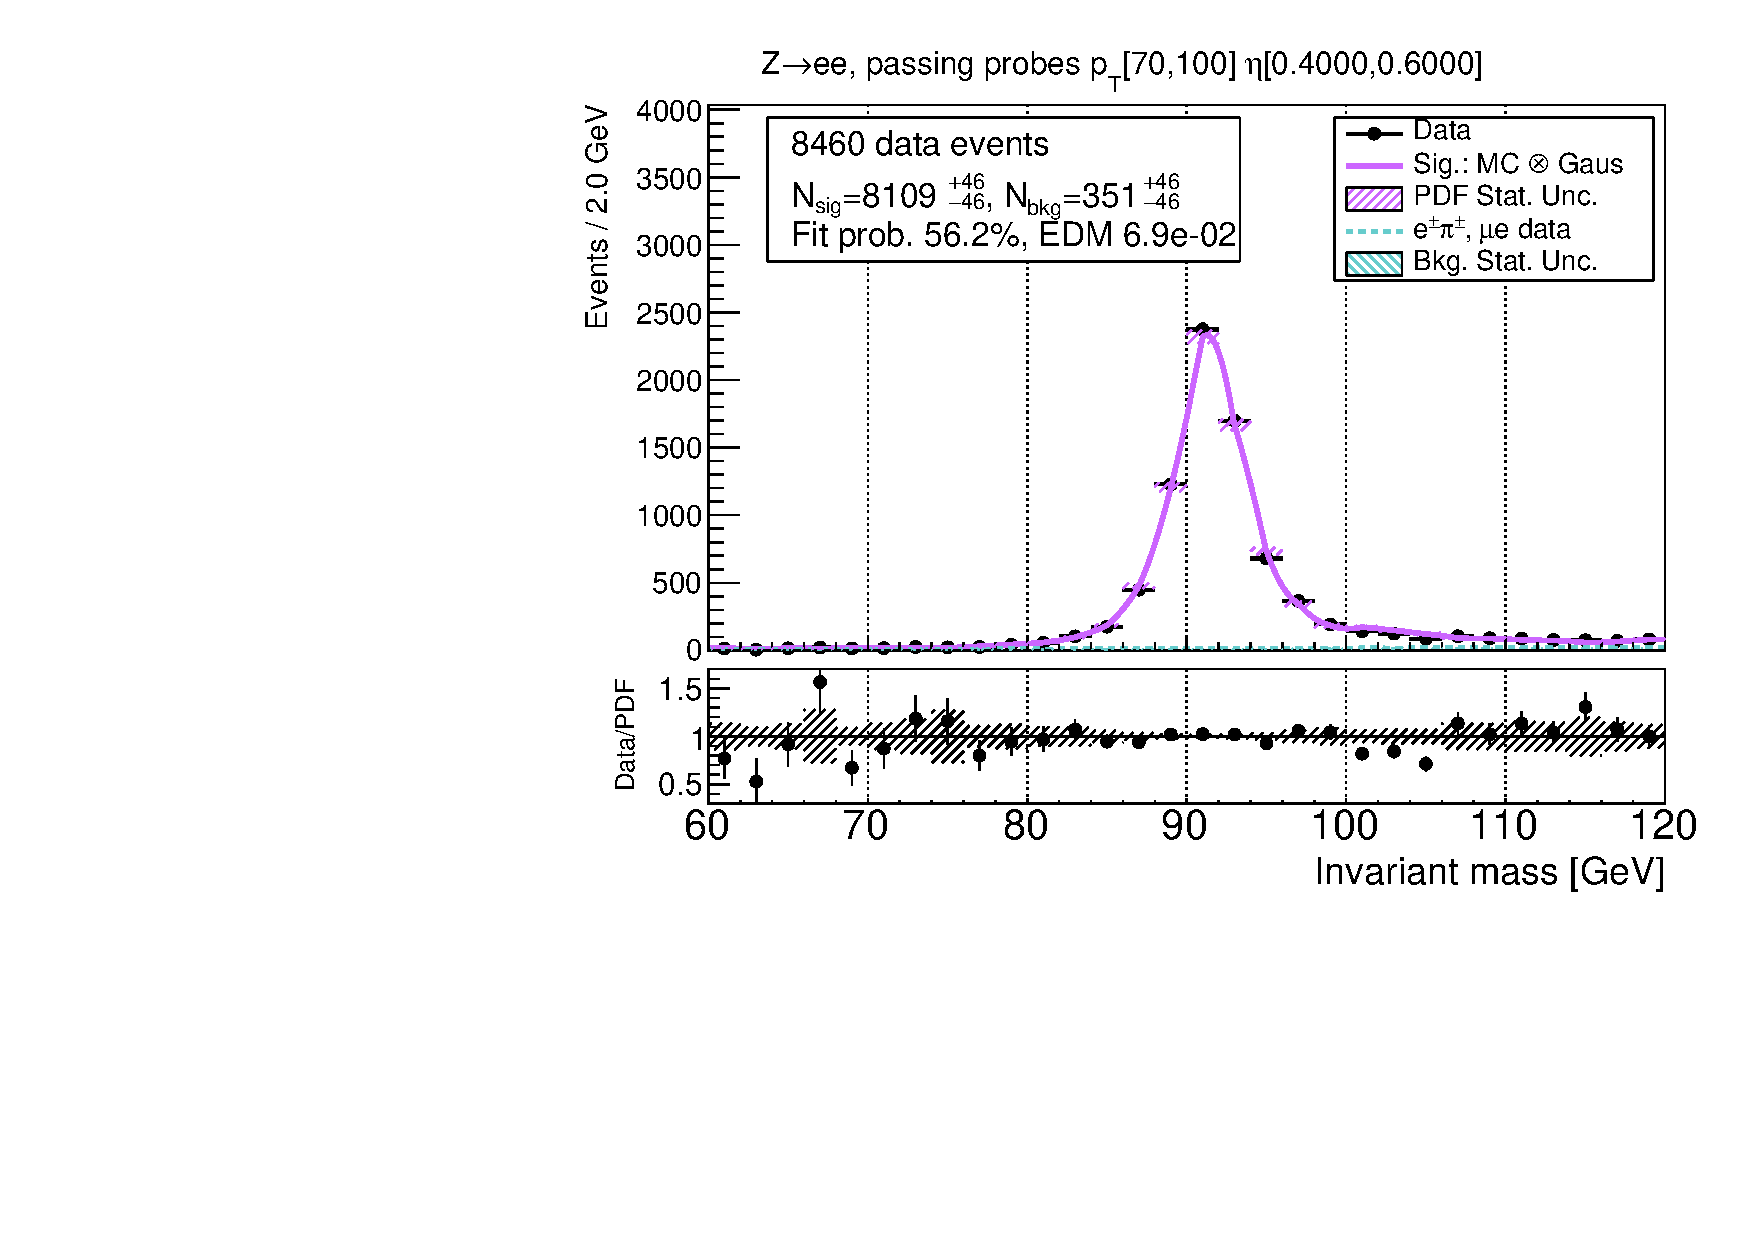
\includegraphics[width=0.49\textwidth]{figures/Zee_RecoTemplate_BkgLPiEMu_pass_ptBin14_etaBin17.pdf}
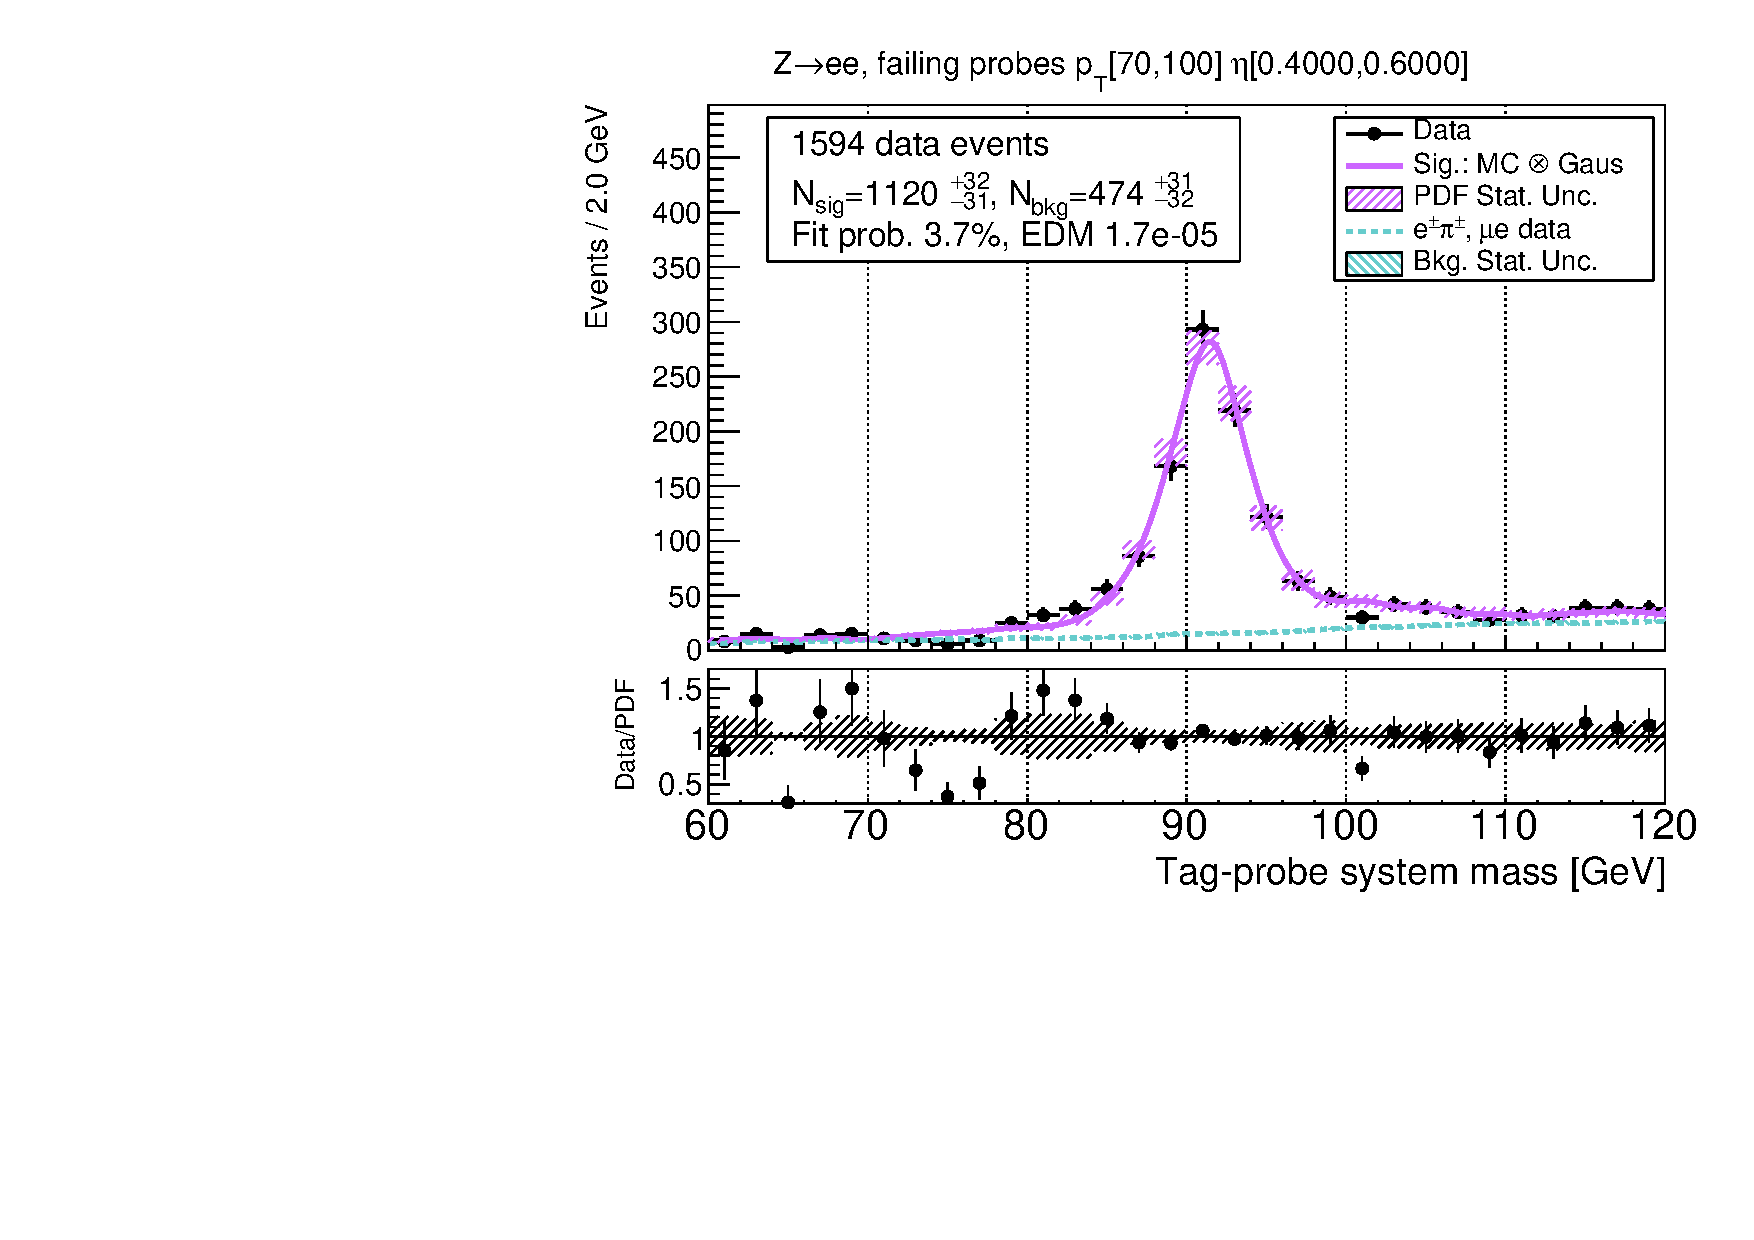
\includegraphics[width=0.49\textwidth]{figures/Zee_RecoTemplate_BkgLPiEMu_fail_ptBin14_etaBin17.pdf}
\caption{Efficiency extraction fits for the Medium electron working point using the data-driven background shape, at higher values of electron transverse momentum.}
\label{fig:ZeeNominalFits2}
\end{figure}

\section{Lepton efficiencies and scale factors}
\textcolor{red}{\bf{MOVE THIS TO APPENDICES?}}
\subsection{Medium muon efficiencies and scale factors}
The extracted data efficiencies are shown in Figure~\ref{fig:ZmmDataEff}.
The MC efficiencies from counting are shown in Figure~\ref{fig:ZmmMCEff}.
The Data/MC efficiency scale factors are shown in Figure~\ref{fig:ZmmScaleFactors}, with
propagated statistical errors in Figures~\ref{fig:ZmmScaleFactorsErrorHi} and~\ref{fig:ZmmScaleFactorsErrorLo}.
The main feature is a drop in the efficiency for low-energy muons in the central detector region.
\begin{figure}
\centering
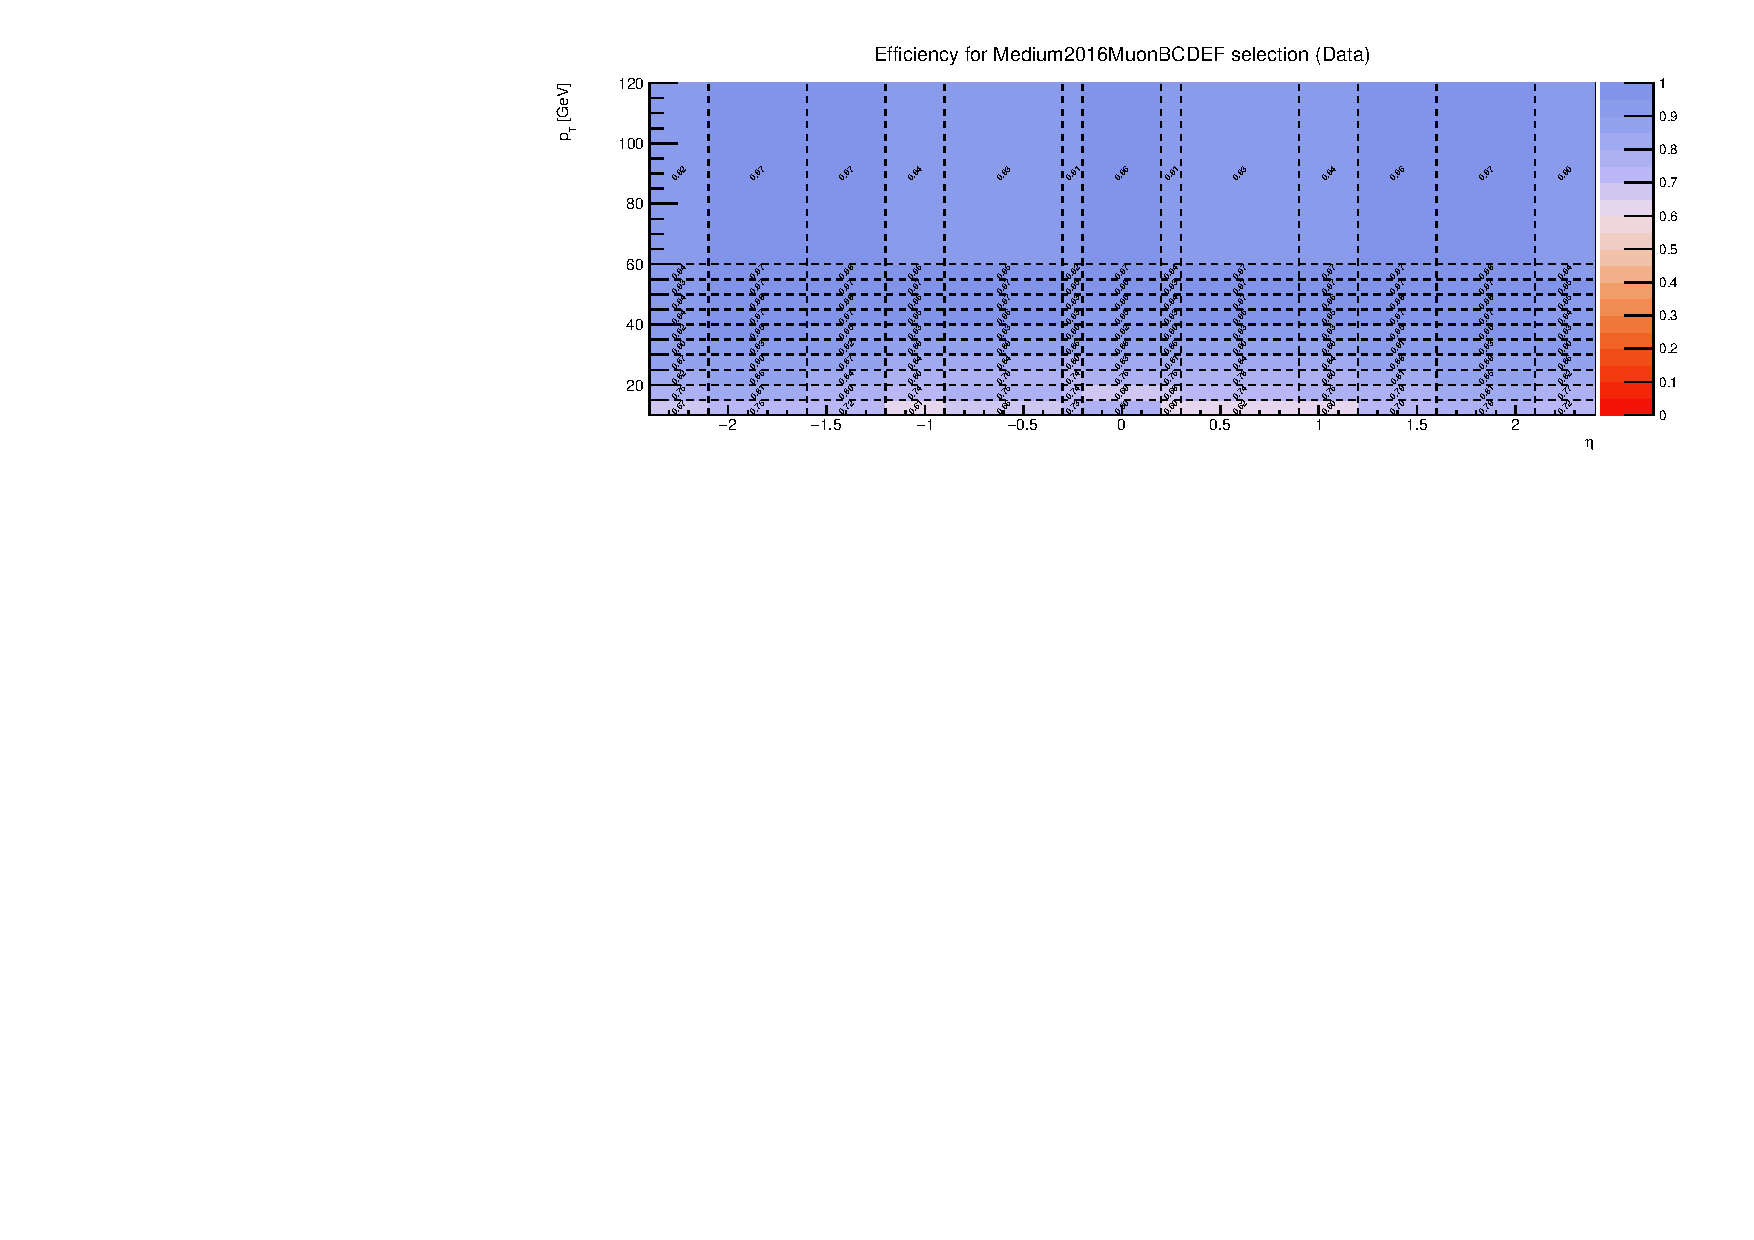
\includegraphics[width=1.00\textwidth]{{figures/eff_data_Medium2016MuonBCDEF_0.0-0.0_10.0-120.0}.pdf}
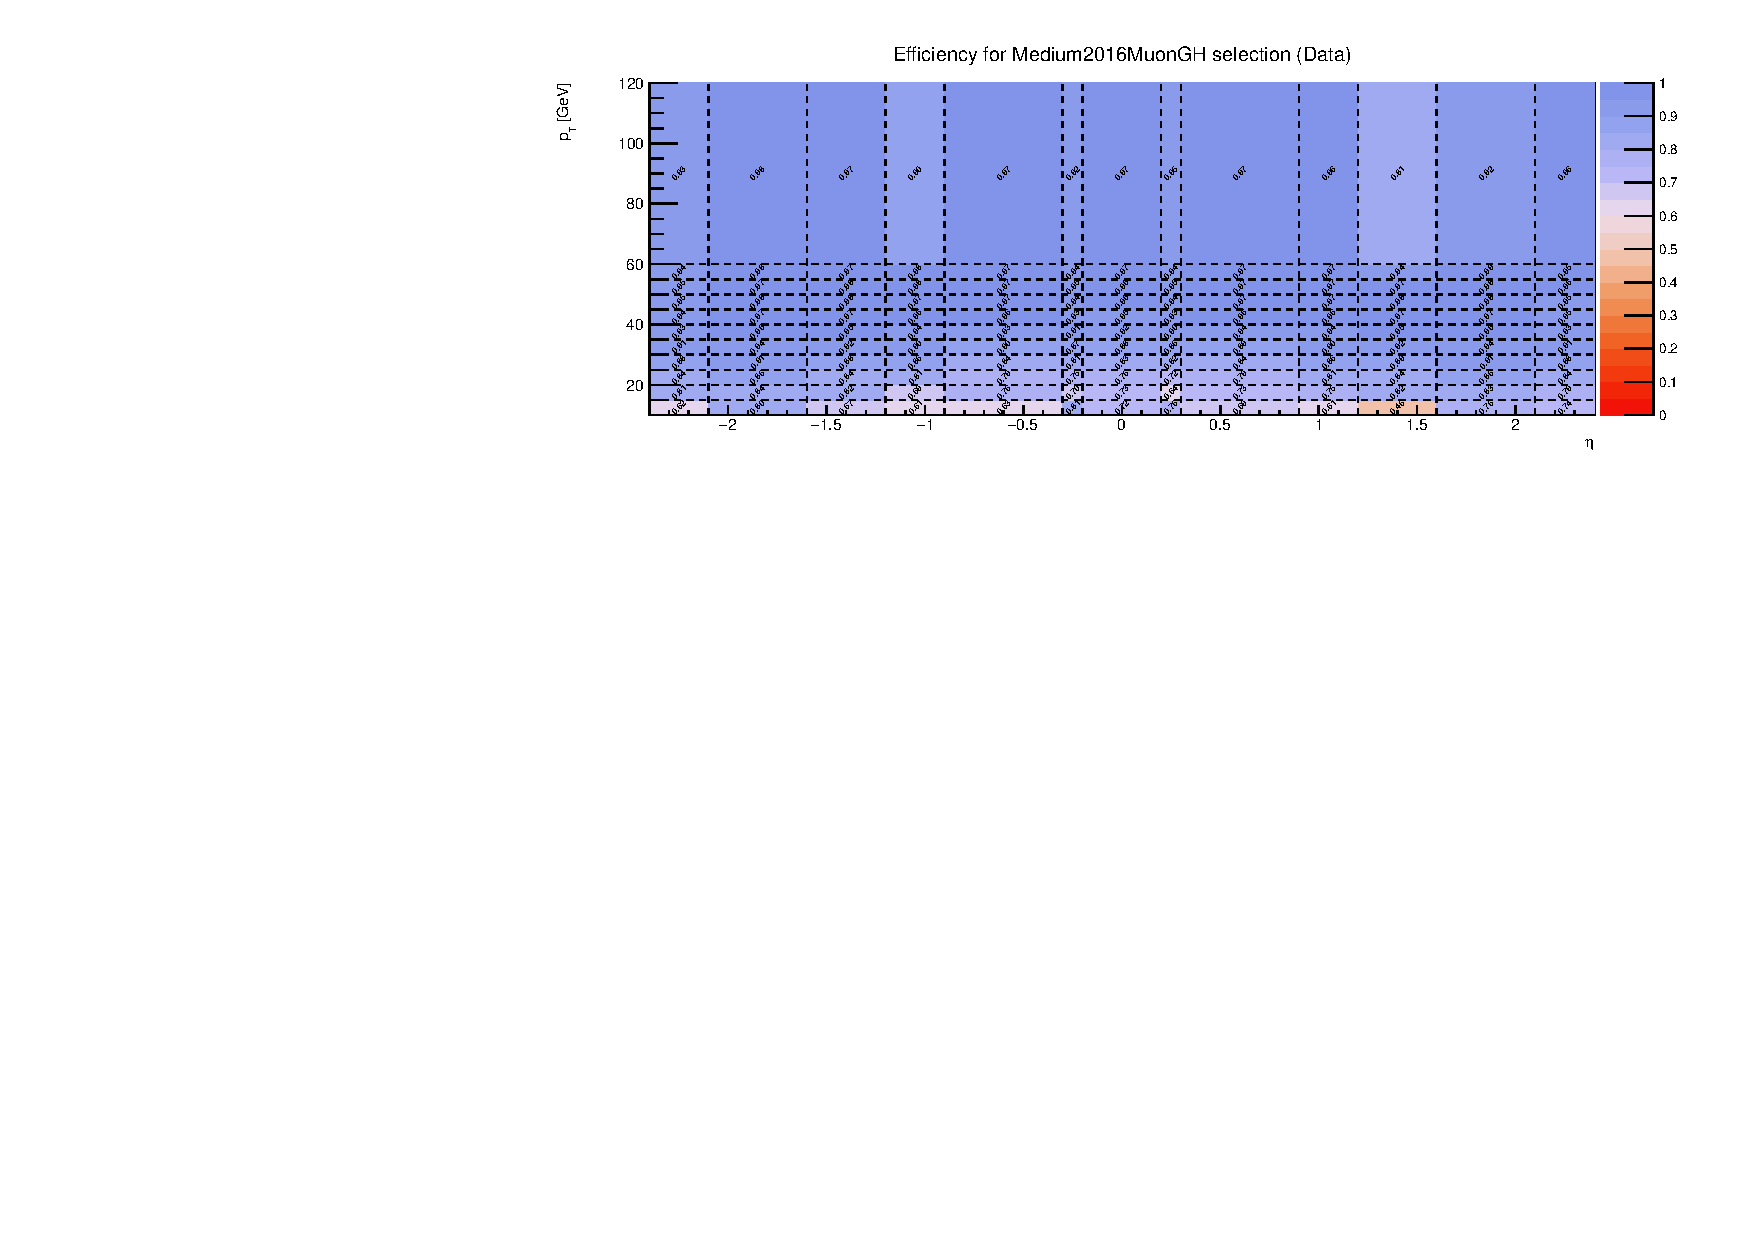
\includegraphics[width=1.00\textwidth]{{figures/eff_data_Medium2016MuonGH_0.0-0.0_10.0-120.0}.pdf}
\caption{Efficiencies extracted from data for the Medium muon working point in 2016 run eras B to F, and G to H.}
\label{fig:ZmmDataEff}
\end{figure}
\begin{figure}
\centering
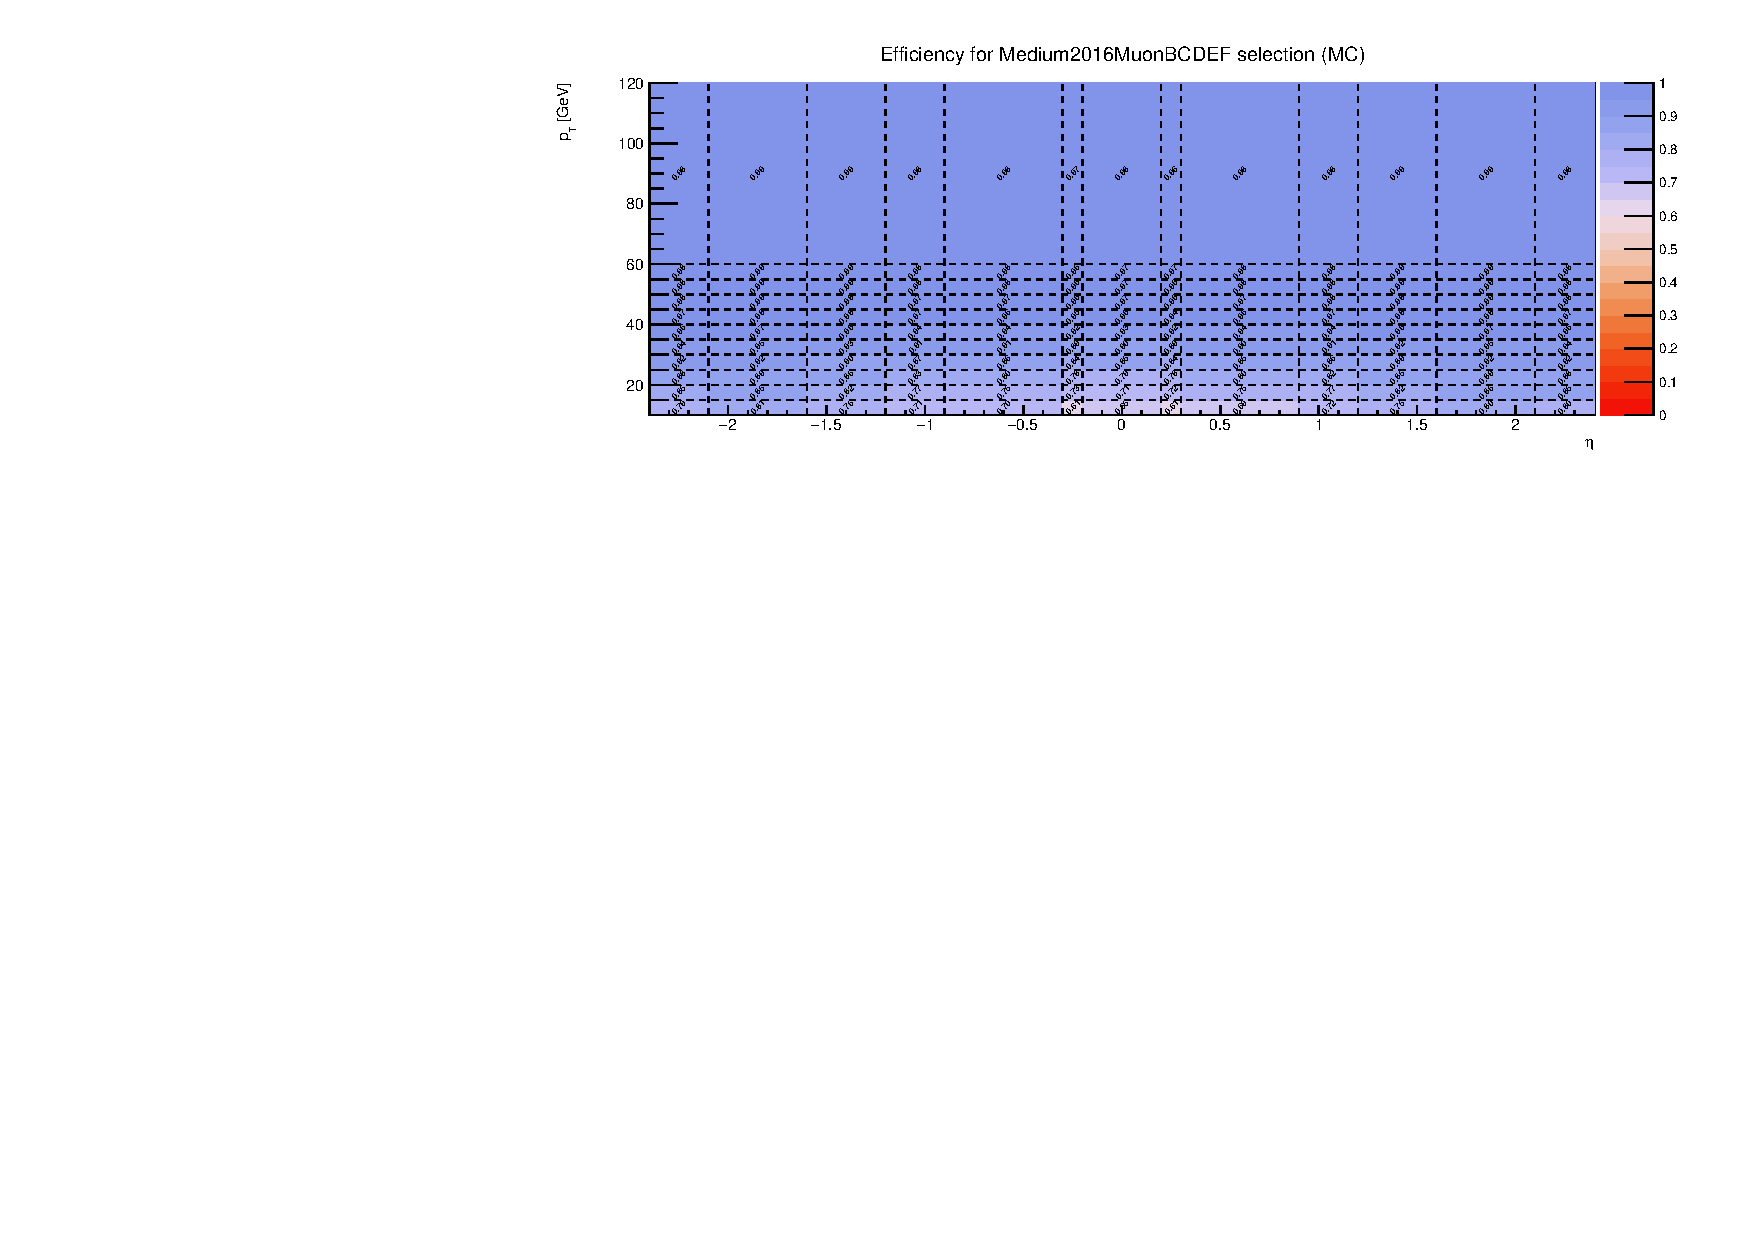
\includegraphics[width=1.00\textwidth]{{figures/eff_mc_Medium2016MuonBCDEF_0.0-0.0_10.0-120.0}.pdf}
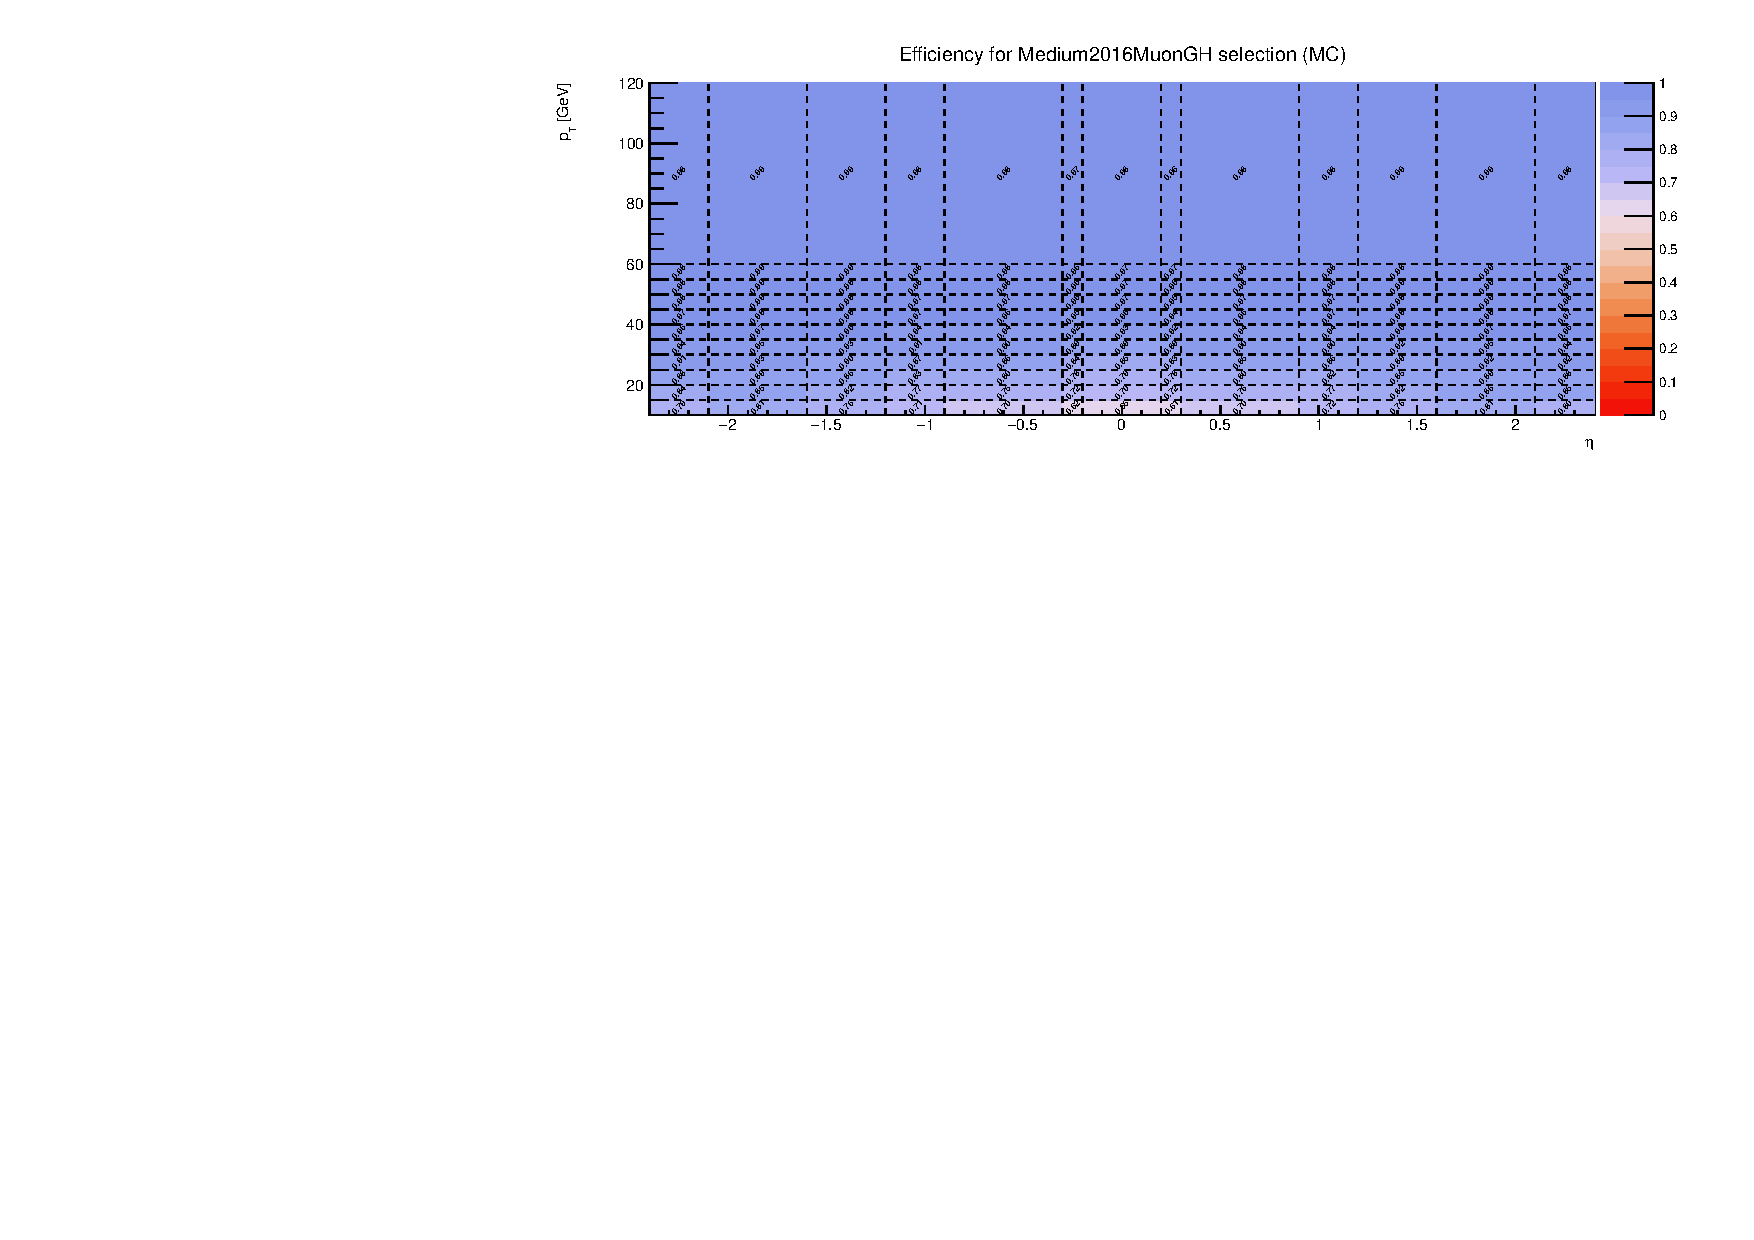
\includegraphics[width=1.00\textwidth]{{figures/eff_mc_Medium2016MuonGH_0.0-0.0_10.0-120.0}.pdf}
\caption{Efficiencies extracted from MC for the Medium muon working point after reweighting to the pileup profile in 2016 run eras B to F, and G to H.}
\label{fig:ZmmMCEff}
\end{figure}
\begin{figure}
\centering
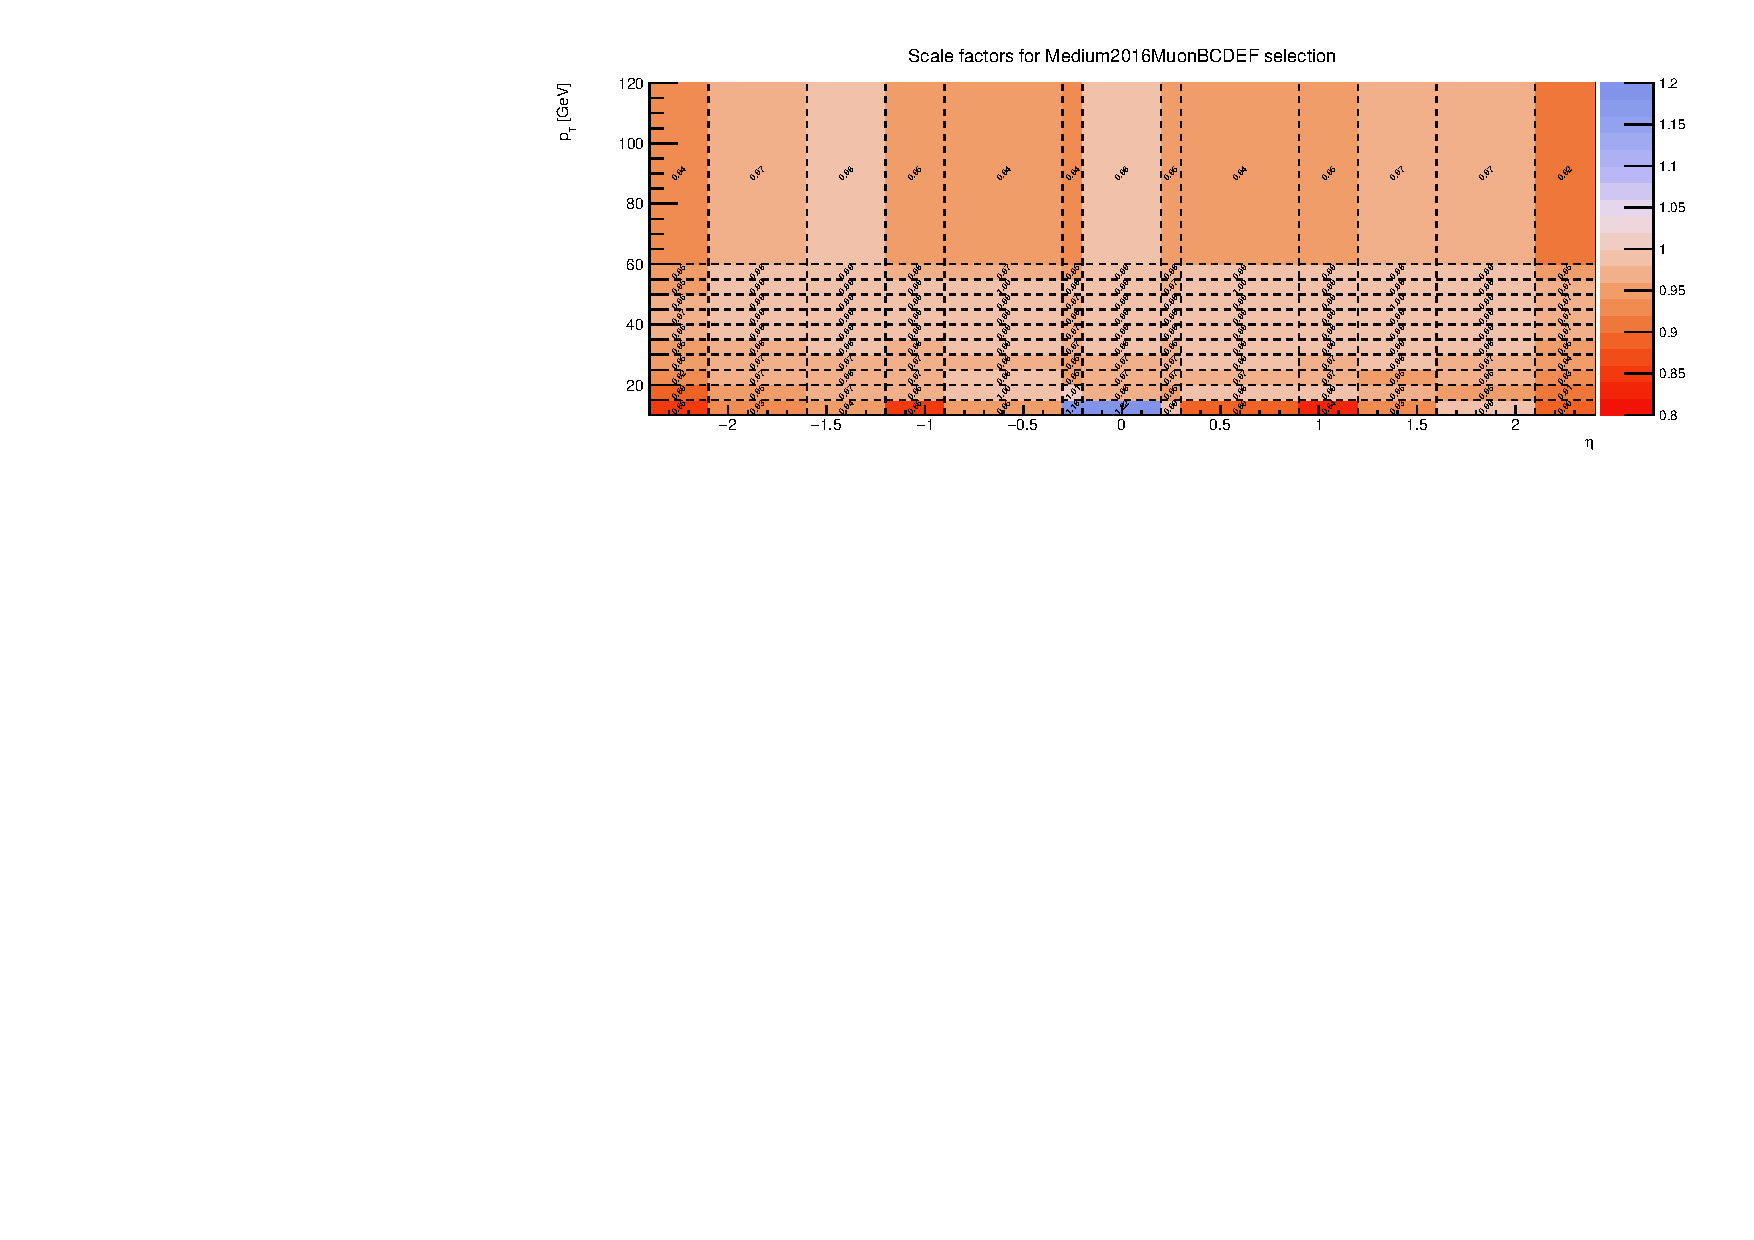
\includegraphics[width=1.00\textwidth]{{figures/scalefactors_Medium2016MuonBCDEF_0.0-0.0_10.0-120.0}.pdf}
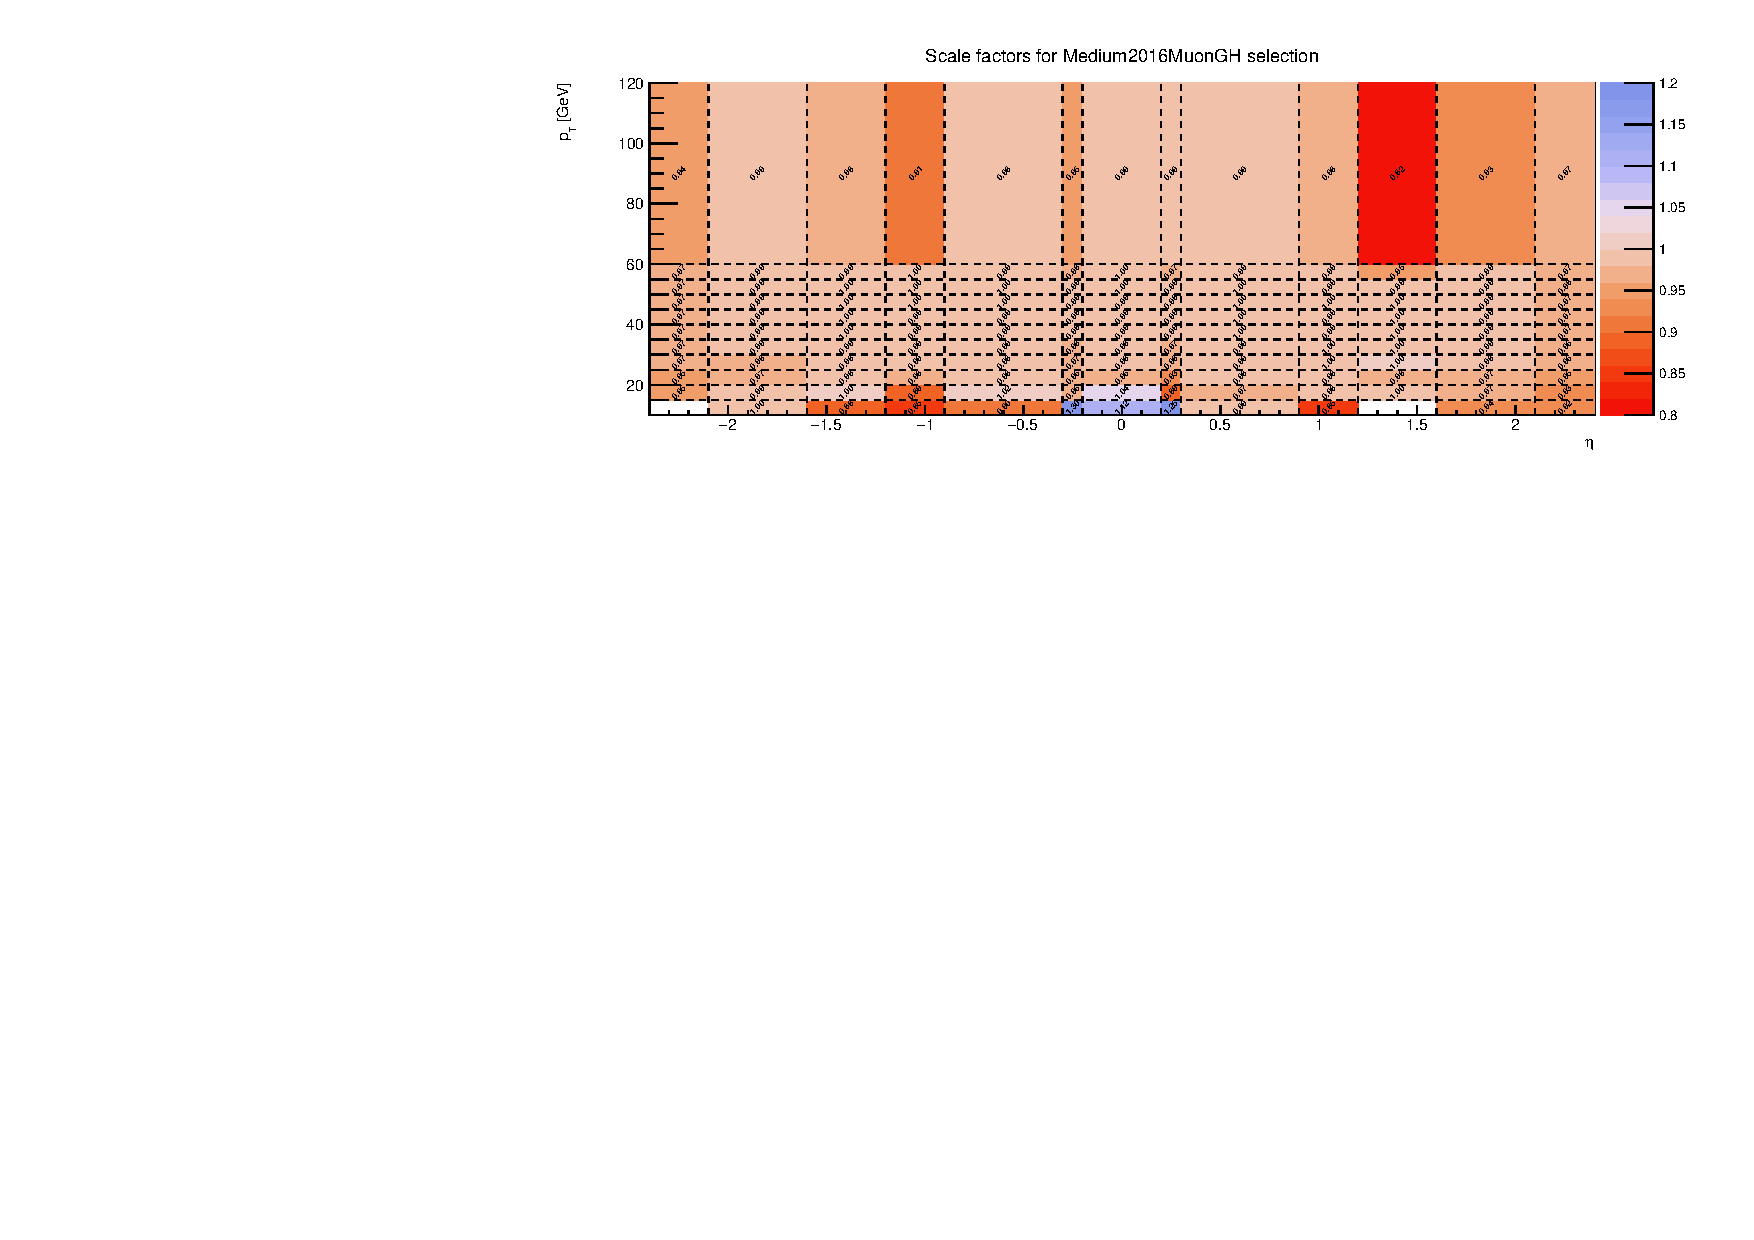
\includegraphics[width=1.00\textwidth]{{figures/scalefactors_Medium2016MuonGH_0.0-0.0_10.0-120.0}.pdf}
\caption{Scale factors derived from Data/MC efficiencies for the Medium muon working point in 2016 run eras B to F, and G to H.}
\label{fig:ZmmScaleFactors}
\end{figure}
\begin{figure}
\centering
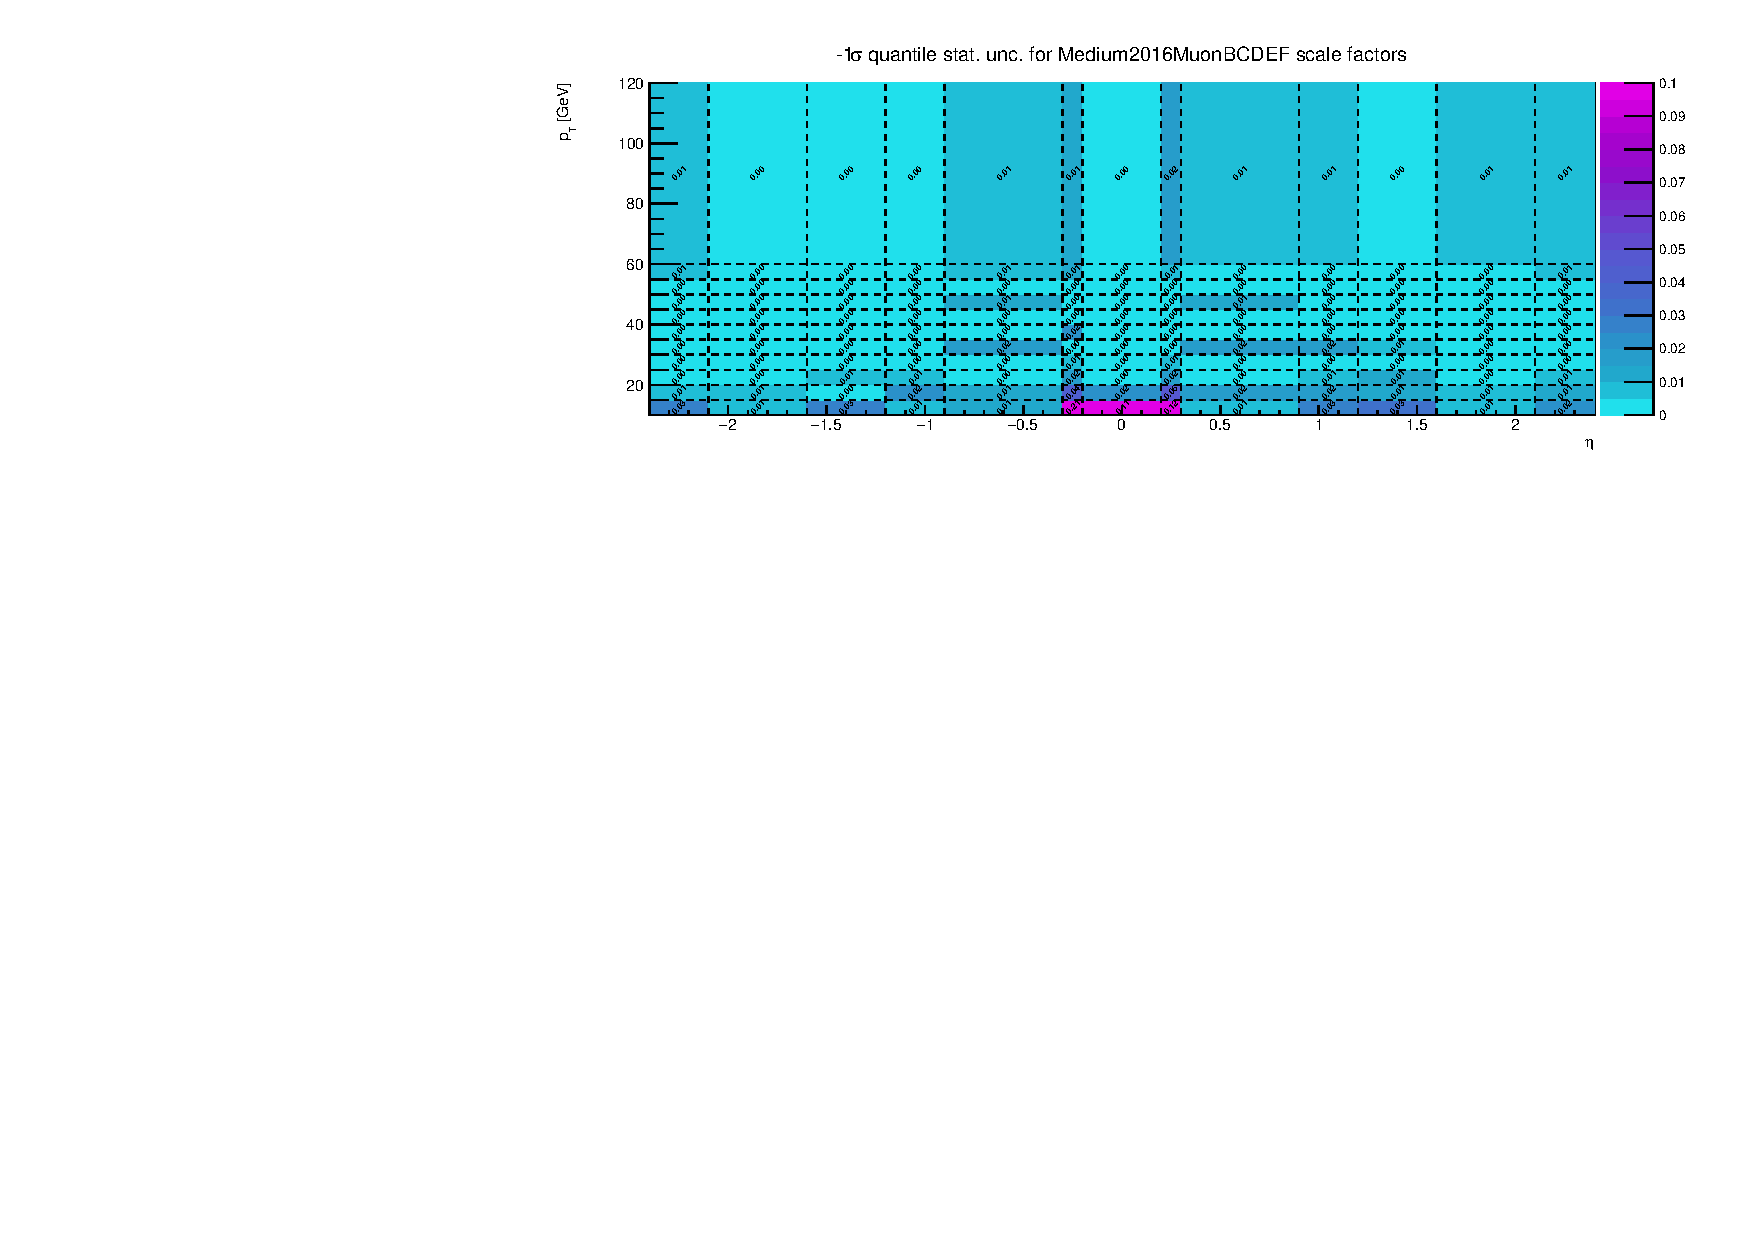
\includegraphics[width=1.00\textwidth]{{figures/scalefactors_Medium2016MuonBCDEF_statErrorLow_0.0-0.0_10.0-120.0}.pdf}
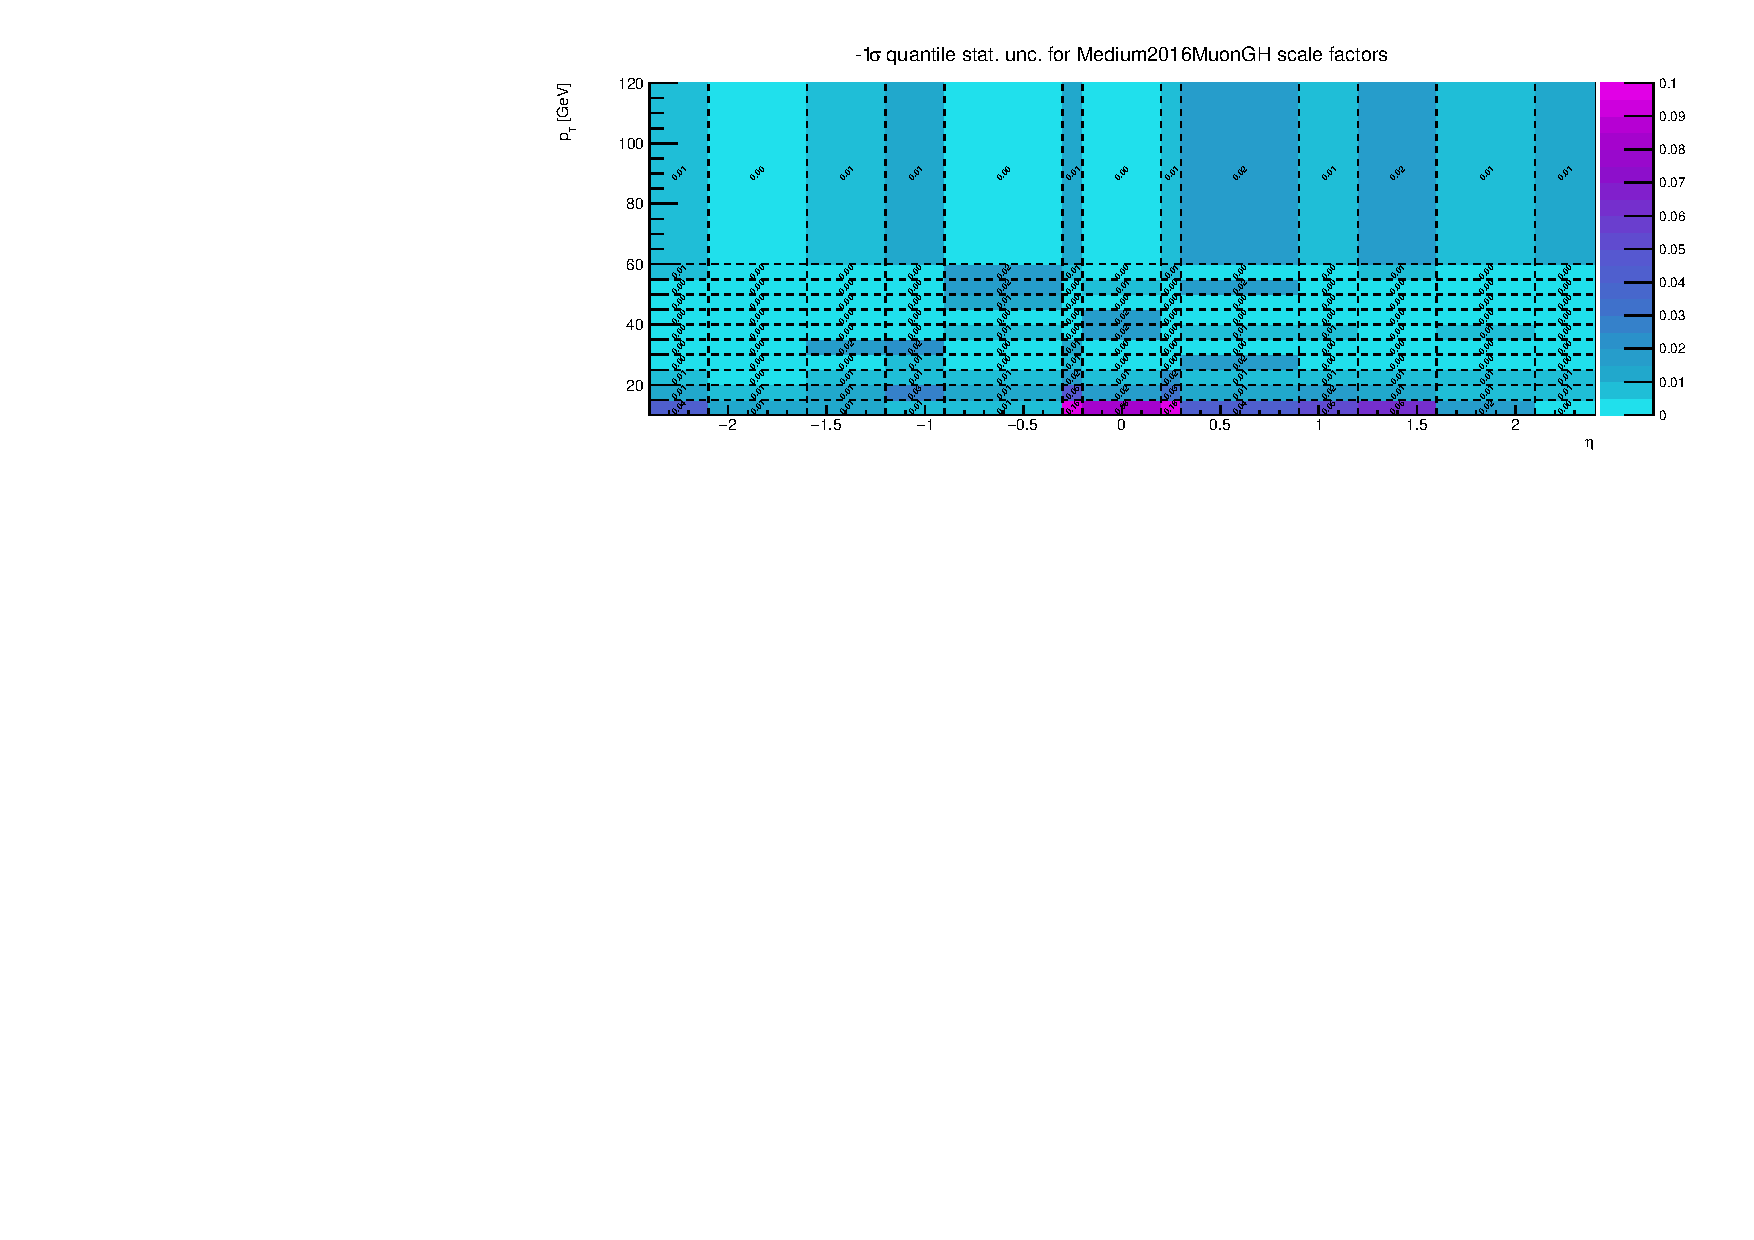
\includegraphics[width=1.00\textwidth]{{figures/scalefactors_Medium2016MuonGH_statErrorLow_0.0-0.0_10.0-120.0}.pdf}
\caption{Statistical uncertainties on the Medium muon scale factors (negative error) in 2016 run eras B to F, and G to H.}
\label{fig:ZmmScaleFactorsErrorHi}
\end{figure}
\begin{figure}
\centering
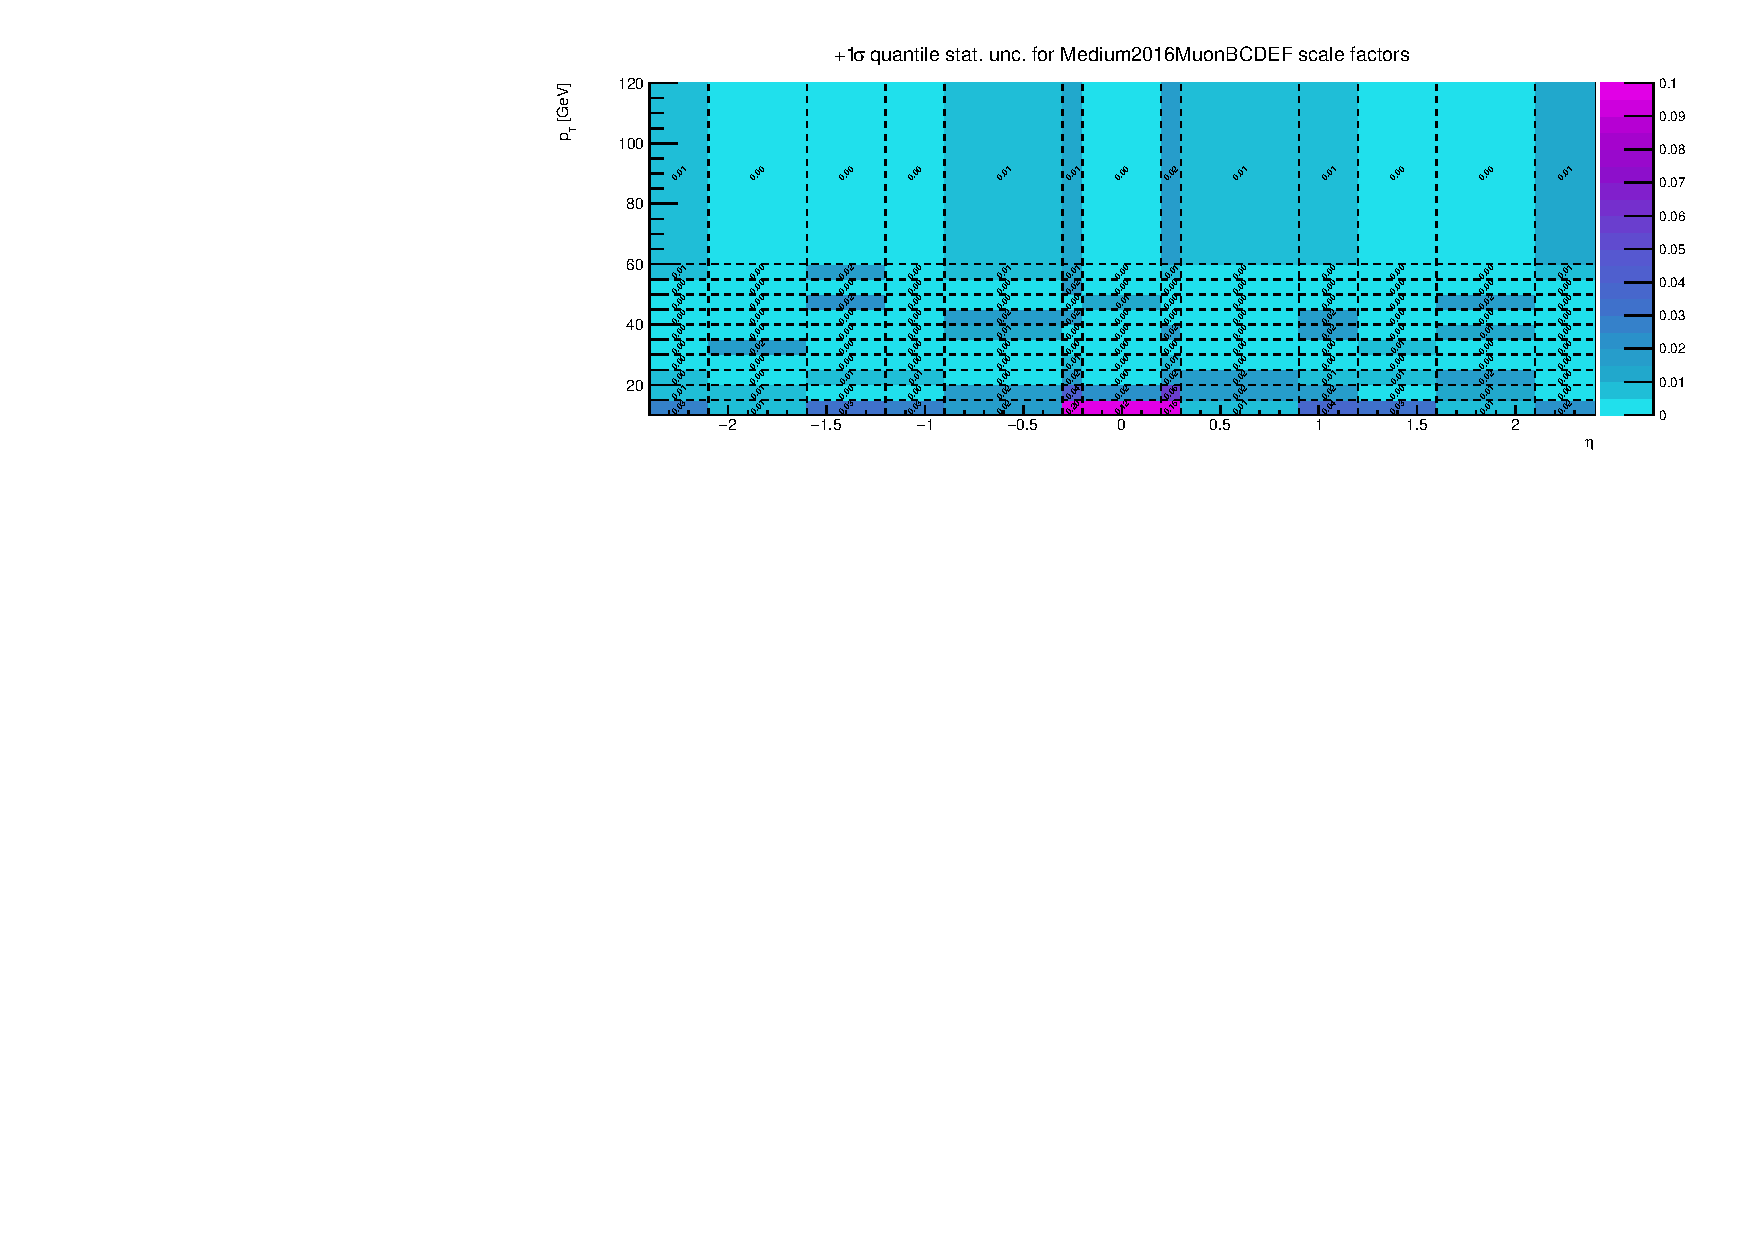
\includegraphics[width=1.00\textwidth]{{figures/scalefactors_Medium2016MuonBCDEF_statErrorHigh_0.0-0.0_10.0-120.0}.pdf}
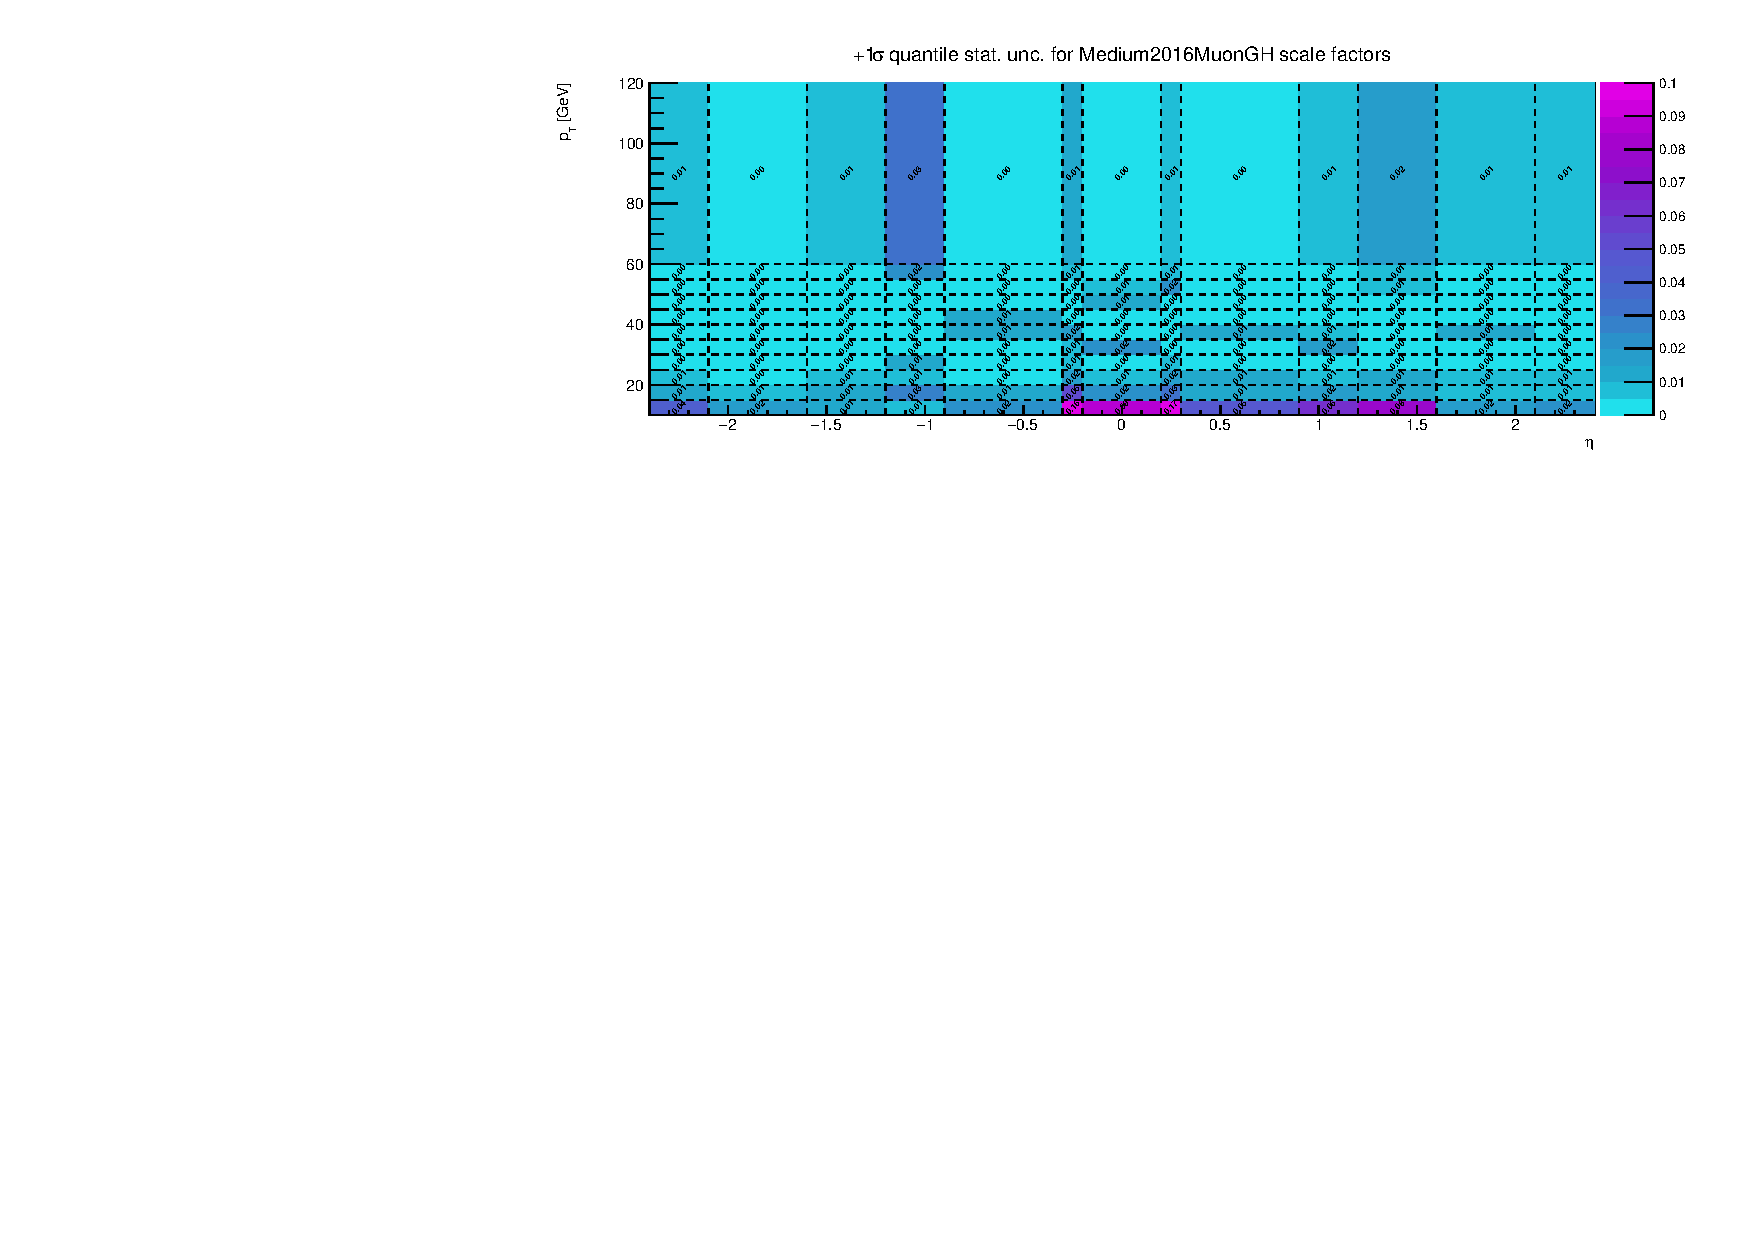
\includegraphics[width=1.00\textwidth]{{figures/scalefactors_Medium2016MuonGH_statErrorHigh_0.0-0.0_10.0-120.0}.pdf}
\caption{Statistical uncertainties on the Medium muon scale factors (positive error) in 2016 run eras B to F, and G to H.}
\label{fig:ZmmScaleFactorsErrorLo}
\end{figure}

\clearpage
\subsection{Medium electron efficiencies and scale factors}
The extracted data efficiencies are shown in Figure~\ref{fig:ZeeDataEff}.
The MC efficiencies from counting are shown in Figure~\ref{fig:ZeeMCEff}.
The Data/MC efficiency scale factors are shown in Figure~\ref{fig:ZeeScaleFactors}, with
propagated statistical errors in Figures~\ref{fig:ZeeScaleFactorsErrorHi} and~\ref{fig:ZeeScaleFactorsErrorLo}.
In general, the efficiencies are lower at lower energies or in the detector endcap ($\abs{\eta}>1.566$).
The scale factors reflect significant asymmetry in positive and negative values of $\eta$ and have a 
nonlinear structure in the endcap.

\begin{figure}
\centering
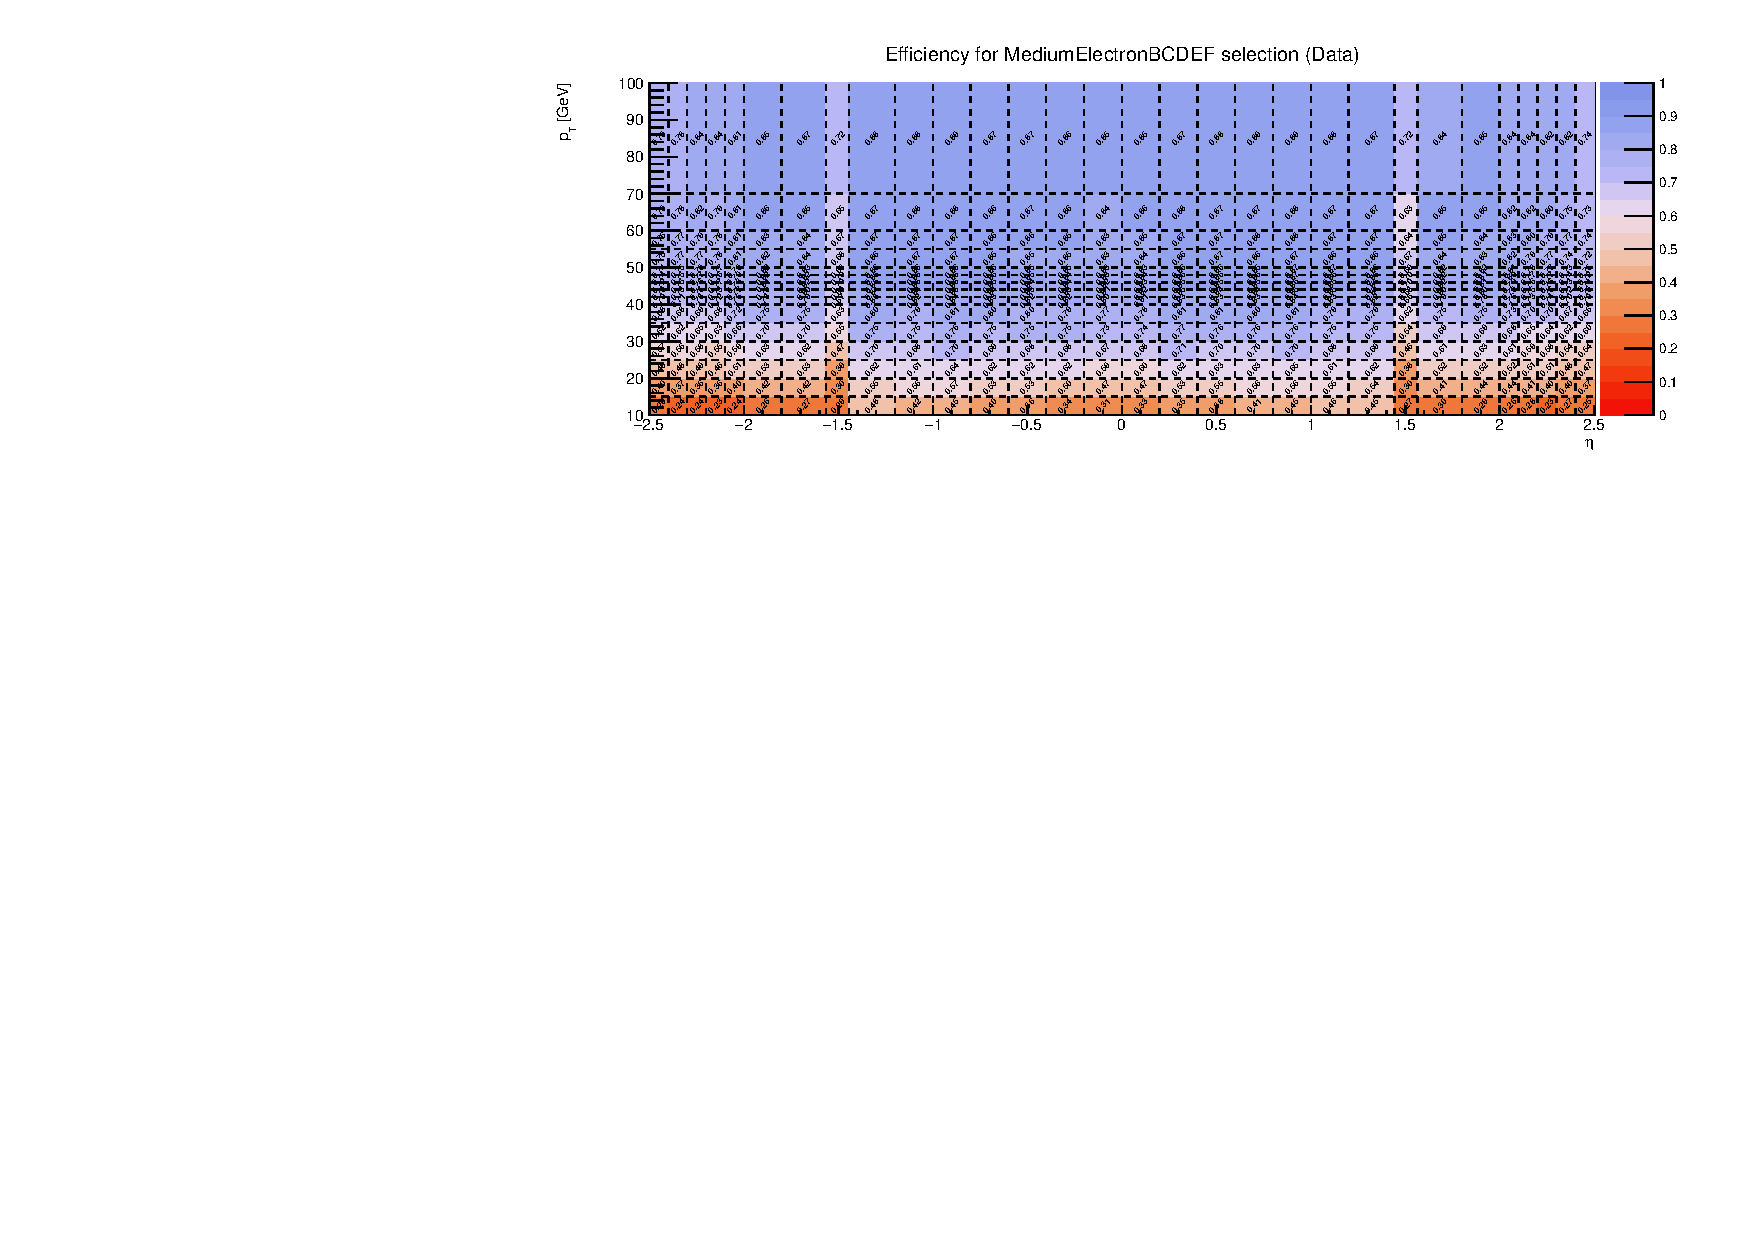
\includegraphics[width=1.00\textwidth]{{figures/eff_data_MediumElectronBCDEF_0.0-0.0_10.0-100.0}.pdf}
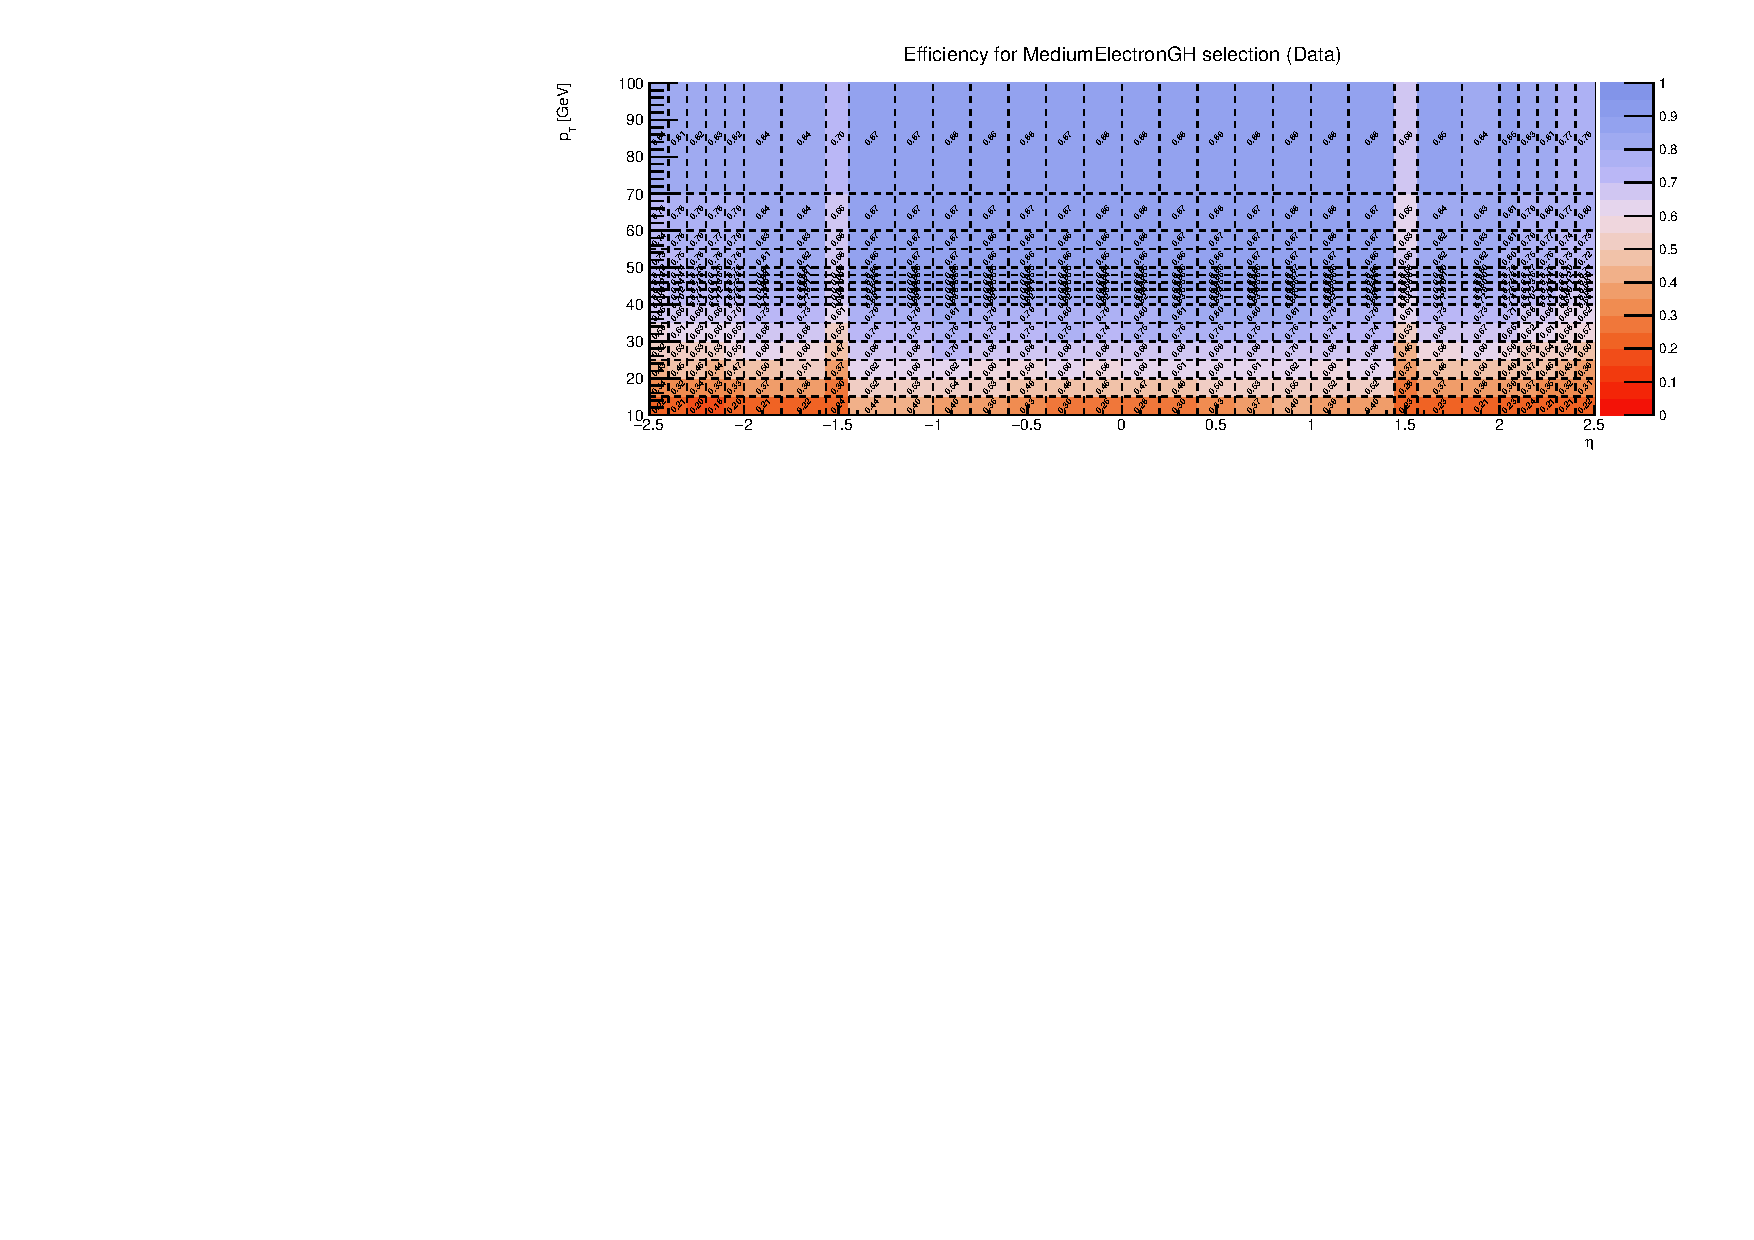
\includegraphics[width=1.00\textwidth]{{figures/eff_data_MediumElectronGH_0.0-0.0_10.0-100.0}.pdf}
\caption{Efficiencies extracted from data for the Medium electron working point in 2016 run eras B to F, and G to H.}
\label{fig:ZeeDataEff}
\end{figure}
\begin{figure}
\centering
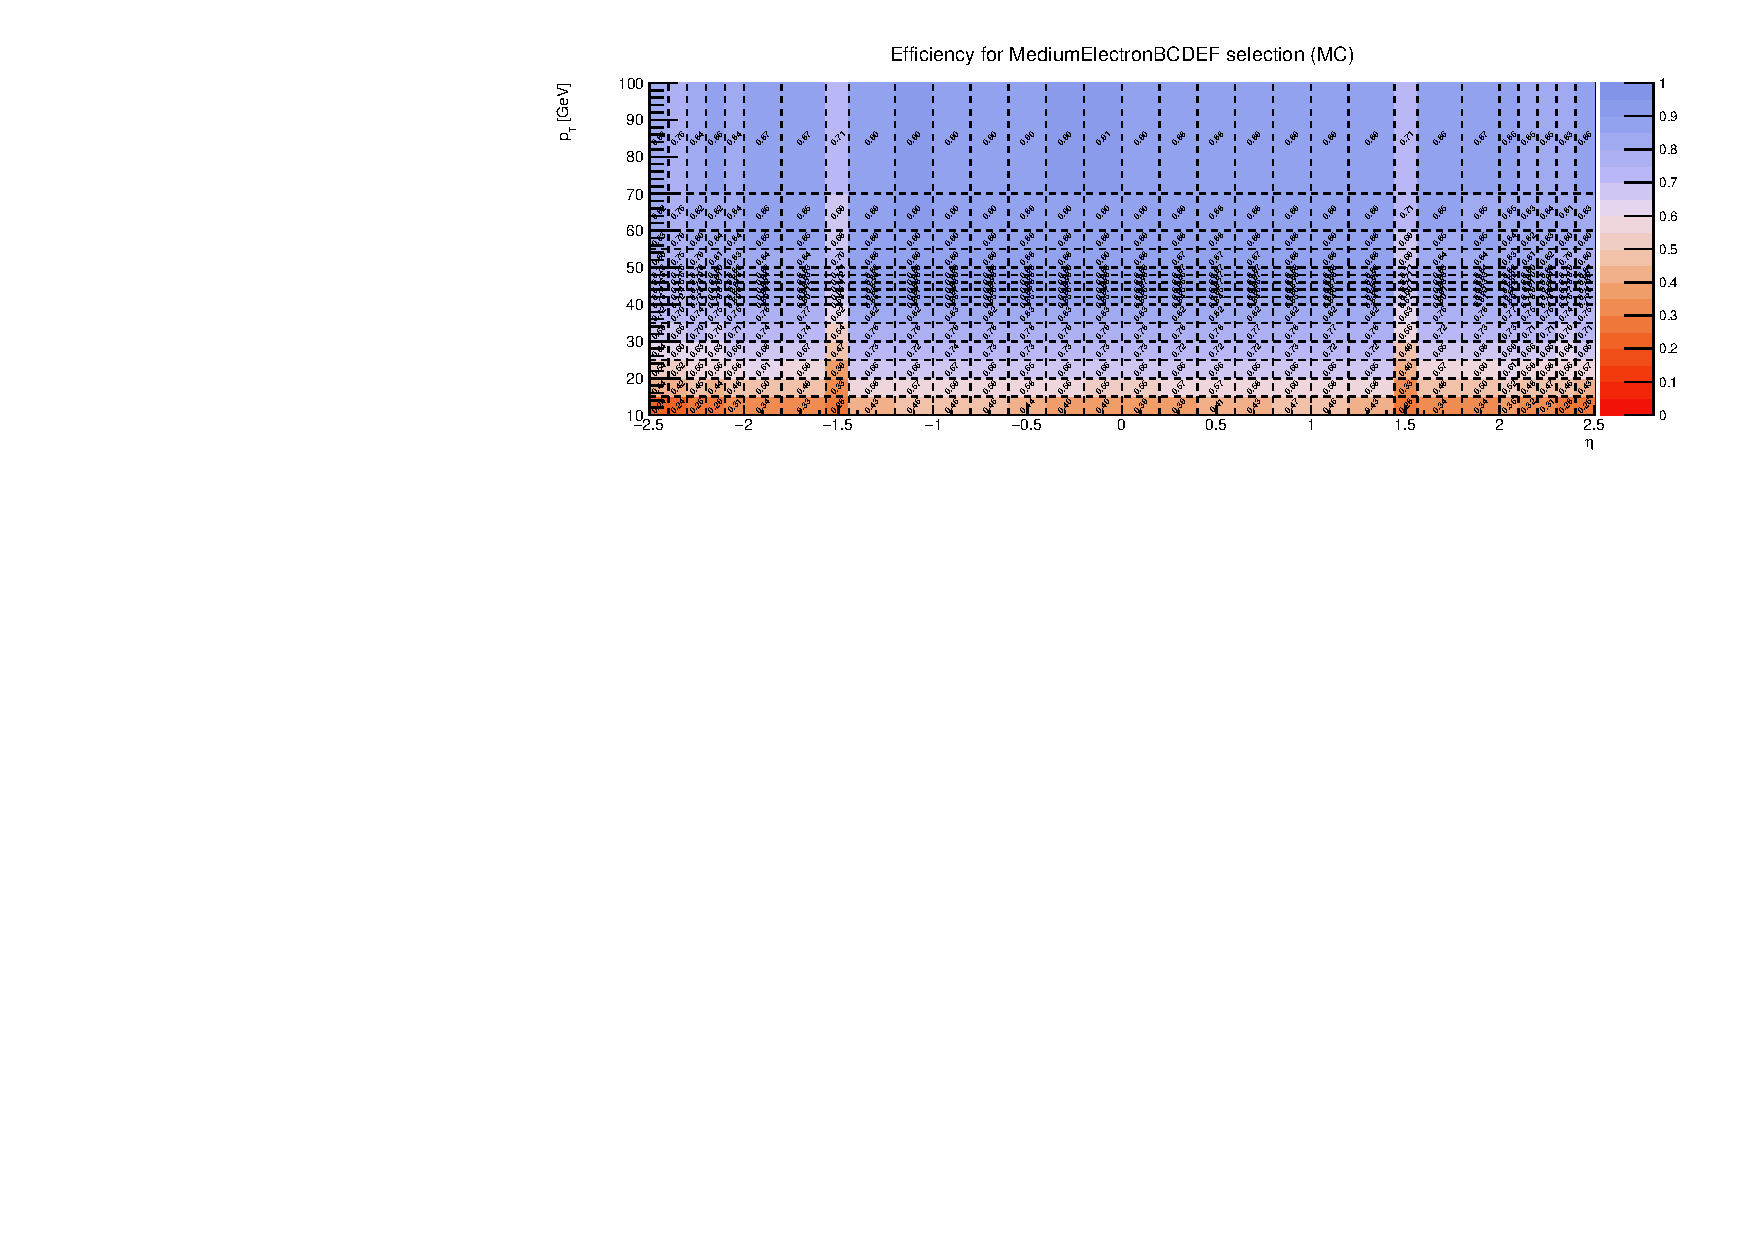
\includegraphics[width=1.00\textwidth]{{figures/eff_mc_MediumElectronBCDEF_0.0-0.0_10.0-100.0}.pdf}
\includegraphics[width=1.00\textwidth]{{figures/eff_mc_MediumElectronGH_0.0-0.0_10.0-100.0}.pdf} 
\caption{Efficiencies extracted from MC for the Medium electron working point after reweighting to the pileup profile in 2016 run eras B to F, and G to H.}
\label{fig:ZeeMCEff}
\end{figure}
\begin{figure}
\centering
\includegraphics[width=1.00\textwidth]{{figures/scalefactors_MediumElectronBCDEF_0.0-0.0_10.0-100.0}.pdf}
\includegraphics[width=1.00\textwidth]{{figures/scalefactors_MediumElectronGH_0.0-0.0_10.0-100.0}.pdf} 
\caption{Scale factors derived from Data/MC efficiencies for the Medium electron working point in 2016 run eras B to F, and G to H.}
\label{fig:ZeeScaleFactors}
\end{figure}
\begin{figure}
\centering
\includegraphics[width=1.00\textwidth]{{figures/scalefactors_MediumElectronBCDEF_statErrorLow_0.0-0.0_10.0-100.0}.pdf}
\includegraphics[width=1.00\textwidth]{{figures/scalefactors_MediumElectronGH_statErrorLow_0.0-0.0_10.0-100.0}.pdf} 
\caption{Statistical uncertainties on the Medium electron scale factors (negative error) in 2016 run eras B to F, and G to H.}
\label{fig:ZeeScaleFactorsErrorHi}
\end{figure}
\begin{figure}
\centering
\includegraphics[width=1.00\textwidth]{{figures/scalefactors_MediumElectronBCDEF_statErrorHigh_0.0-0.0_10.0-100.0}.pdf}
\includegraphics[width=1.00\textwidth]{{figures/scalefactors_MediumElectronGH_statErrorHigh_0.0-0.0_10.0-100.0}.pdf} 
\caption{Statistical uncertainties on the Medium electron scale factors (positive error) in 2016 run eras B to F, and G to H.}
\label{fig:ZeeScaleFactorsErrorLo}
\end{figure}

\section{Assessment of systematic uncertainty}
\label{sec:tnpsyst}
In this section, we quantify the systematic uncertainty arising from five distinct sources related to our ignorance
of the true signal and background shapes, the generator-related uncertainty, and possible selection bias.
In each case, the absolute difference between two alternative methods is taken as the systematic uncertainty.
\subsection{Background shape modeling}
To quantify the uncertainty in deriving the background shape from the data-driven method,
we use an analytic function as an alternative background shape.
The function chosen is a linear combination of: a decaying exponential to model low-energy fakes,
and a wide Gaussian with exponential tails to represent the peaking structure
sculpted by applying energy cuts to a falling combinatorial background mass distribution.
Previously, an error function multiplied with a decaying exponential was used, but this function
has problems related to fit convergence due to poor parameterization.

Examples of fits for 2016 run eras B to F with the analytic background are shown for dimuons in
Figures ~\ref{fig:ZmmAltBkgFits1} and~\ref{fig:ZmmAltBkgFits2}, 
and for dielectrons in Figures~\ref{fig:ZeeAltBkgFits1} and~\ref{fig:ZeeAltBkgFits2}.
These may be compared with the fits using the data-driven background shape 
in section \ref{sec:tnpfits}.
The difference in the Data/MC scale factors derived using the two methods is taken as a systematic; 
see Figures~\ref{fig:ZmmSystBkgModel} and~\ref{fig:ZeeSystBkgModel}.

\begin{figure}
\centering
\includegraphics[width=0.49\textwidth]{figures/Zmm_RecoTemplate_BkgAnalytic_pass_ptBin0_etaBin1.pdf}
\includegraphics[width=0.49\textwidth]{figures/Zmm_RecoTemplate_BkgAnalytic_fail_ptBin0_etaBin1.pdf}
\includegraphics[width=0.49\textwidth]{figures/Zmm_RecoTemplate_BkgAnalytic_pass_ptBin1_etaBin9.pdf}
\includegraphics[width=0.49\textwidth]{figures/Zmm_RecoTemplate_BkgAnalytic_fail_ptBin1_etaBin9.pdf}
\caption{Efficiency extraction fits for the Medium muon working point using the alternative analytic background shape, at low muon transverse momentum.}
\label{fig:ZmmAltBkgFits1}
\end{figure}

\begin{figure}
\centering
\includegraphics[width=0.49\textwidth]{figures/Zmm_RecoTemplate_BkgAnalytic_pass_ptBin7_etaBin0.pdf}
\includegraphics[width=0.49\textwidth]{figures/Zmm_RecoTemplate_BkgAnalytic_fail_ptBin7_etaBin0.pdf}
\includegraphics[width=0.49\textwidth]{figures/Zmm_RecoTemplate_BkgAnalytic_pass_ptBin10_etaBin6.pdf}
\includegraphics[width=0.49\textwidth]{figures/Zmm_RecoTemplate_BkgAnalytic_fail_ptBin10_etaBin6.pdf}
\caption{Efficiency extraction fits for the Medium muon working point using the alternative analytic background shape, at higher values of muon transverse momentum.}
\label{fig:ZmmAltBkgFits2}
\end{figure}

\begin{figure}
\centering
\includegraphics[width=0.49\textwidth]{figures/Zee_RecoTemplate_BkgAnalytic_pass_ptBin0_etaBin0.pdf}
\includegraphics[width=0.49\textwidth]{figures/Zee_RecoTemplate_BkgAnalytic_fail_ptBin0_etaBin0.pdf}
\includegraphics[width=0.49\textwidth]{figures/Zee_RecoTemplate_BkgAnalytic_pass_ptBin1_etaBin19.pdf}
\includegraphics[width=0.49\textwidth]{figures/Zee_RecoTemplate_BkgAnalytic_fail_ptBin1_etaBin19.pdf}
\caption{Efficiency extraction fits for the Medium electron working point using the alternative analytic background shape, at low electron transverse momentum.}
\label{fig:ZeeAltBkgFits1}
\end{figure}

\begin{figure}
\centering
\includegraphics[width=0.49\textwidth]{figures/Zee_RecoTemplate_BkgAnalytic_pass_ptBin3_etaBin23.pdf}
\includegraphics[width=0.49\textwidth]{figures/Zee_RecoTemplate_BkgAnalytic_fail_ptBin3_etaBin23.pdf}
\includegraphics[width=0.49\textwidth]{figures/Zee_RecoTemplate_BkgAnalytic_pass_ptBin14_etaBin17.pdf}
\includegraphics[width=0.49\textwidth]{figures/Zee_RecoTemplate_BkgAnalytic_fail_ptBin14_etaBin17.pdf}
\caption{Efficiency extraction fits for the Medium electron working point using the alternative analytic background shape, at higher values of electron transverse momentum.}
\label{fig:ZeeAltBkgFits2}
\end{figure}

\begin{figure}
\centering
\includegraphics[width=1.00\textwidth]{{figures/scalefactors_Medium2016MuonBCDEF_AltBkg_0.0-0.0_10.0-120.0}.pdf}
\includegraphics[width=1.00\textwidth]{{figures/scalefactors_Medium2016MuonGH_AltBkg_0.0-0.0_10.0-120.0}.pdf} 
\caption{Systematic uncertainties from choice of background model for the Medium muon scale factors in 2016 run eras B to F (top), and G to H (bottom).}
\label{fig:ZmmSystBkgModel}
\end{figure}

\begin{figure}
\centering
\includegraphics[width=1.00\textwidth]{{figures/scalefactors_MediumElectronBCDEF_AltBkg_0.0-0.0_10.0-100.0}.pdf}
\includegraphics[width=1.00\textwidth]{{figures/scalefactors_MediumElectronGH_AltBkg_0.0-0.0_10.0-100.0}.pdf} 
\caption{Systematic uncertainties from choice of background model for the Medium electron scale factors in 2016 run eras B to F (top), and G to H (bottom).}
\label{fig:ZeeSystBkgModel}
\end{figure}
\clearpage
\subsection{Signal resolution modeling}
We consider the uncertainty from using the simulation of the reconstructed Z resonance signal shape
by convolution with an analytic function more complex than a Gaussian to try to capture more detector resolution effects.
The difference in scale factors derived from the data efficiency extraction fits using the two methods
is taken as the systematic uncertainty due to signal resolution modeling.
The alternative function is a single Gaussian with asymmetric, exponential tails.

Examples of fits for 2016 run eras B to F with the alternative resolution function are shown for dimuons in
Figures ~\ref{fig:ZmmAltSigResFits1} and~\ref{fig:ZmmAltSigResFits2}, 
and for dielectrons in Figures~\ref{fig:ZeeAltSigResFits1} and~\ref{fig:ZeeAltSigResFits2}.
These may be compared with the fits using the nominal resolution function
in section \ref{sec:tnpfits}.
The difference in the Data/MC scale factors derived using the two methods is taken as a systematic; 
see Figures~\ref{fig:ZmmSystSigRes} and~\ref{fig:ZeeSystSigRes}.

\begin{figure}
\centering
\includegraphics[width=0.49\textwidth]{figures/Zmm_ResFunc_BkgLPi_pass_ptBin0_etaBin1.pdf}
\includegraphics[width=0.49\textwidth]{figures/Zmm_ResFunc_BkgLPi_fail_ptBin0_etaBin1.pdf}
\includegraphics[width=0.49\textwidth]{figures/Zmm_ResFunc_BkgLPi_pass_ptBin1_etaBin9.pdf}
\includegraphics[width=0.49\textwidth]{figures/Zmm_ResFunc_BkgLPi_fail_ptBin1_etaBin9.pdf}
\caption{Efficiency extraction fits for the Medium muon working point using the analytic detector resolution function, at low muon transverse momentum.}
\label{fig:ZmmAltSigResFits1}
\end{figure}

\begin{figure}
\centering
\includegraphics[width=0.49\textwidth]{figures/Zmm_ResFunc_BkgLPi_pass_ptBin7_etaBin0.pdf}
\includegraphics[width=0.49\textwidth]{figures/Zmm_ResFunc_BkgLPi_fail_ptBin7_etaBin0.pdf}
\includegraphics[width=0.49\textwidth]{figures/Zmm_ResFunc_BkgLPi_pass_ptBin10_etaBin6.pdf}
\includegraphics[width=0.49\textwidth]{figures/Zmm_ResFunc_BkgLPi_fail_ptBin10_etaBin6.pdf}
\caption{Efficiency extraction fits for the Medium muon working point using the analytic detector resolution function, at higher values of muon transverse momentum.}
\label{fig:ZmmAltSigResFits2}
\end{figure}

\begin{figure}
\centering
\includegraphics[width=0.49\textwidth]{figures/Zee_ResFunc_BkgLPiEMu_pass_ptBin0_etaBin0.pdf}
\includegraphics[width=0.49\textwidth]{figures/Zee_ResFunc_BkgLPiEMu_fail_ptBin0_etaBin0.pdf}
\includegraphics[width=0.49\textwidth]{figures/Zee_ResFunc_BkgLPiEMu_pass_ptBin1_etaBin19.pdf}
\includegraphics[width=0.49\textwidth]{figures/Zee_ResFunc_BkgLPiEMu_fail_ptBin1_etaBin19.pdf}
\caption{Efficiency extraction fits for the Medium electron working point using the analytic detector resolution function, at low electron transverse momentum.}
\label{fig:ZeeAltSigResFits1}
\end{figure}

\begin{figure}
\centering
\includegraphics[width=0.49\textwidth]{figures/Zee_ResFunc_BkgLPiEMu_pass_ptBin3_etaBin23.pdf}
\includegraphics[width=0.49\textwidth]{figures/Zee_ResFunc_BkgLPiEMu_fail_ptBin3_etaBin23.pdf}
\includegraphics[width=0.49\textwidth]{figures/Zee_ResFunc_BkgLPiEMu_pass_ptBin14_etaBin17.pdf}
\includegraphics[width=0.49\textwidth]{figures/Zee_ResFunc_BkgLPiEMu_fail_ptBin14_etaBin17.pdf}
\caption{Efficiency extraction fits for the Medium electron working point using the analytic detector resolution function, at higher values of electron transverse momentum.}
\label{fig:ZeeAltSigResFits2}
\end{figure}

\begin{figure}
\centering
\includegraphics[width=1.00\textwidth]{{figures/scalefactors_Medium2016MuonBCDEF_ResFunc_0.0-0.0_10.0-120.0}.pdf}
\includegraphics[width=1.00\textwidth]{{figures/scalefactors_Medium2016MuonGH_ResFunc_0.0-0.0_10.0-120.0}.pdf} 
\caption{Systematic uncertainties from signal resolution modeling for the Medium muon scale factors in 2016 run eras B to F (top), and G to H (bottom).}
\label{fig:ZmmSystSigRes}
\end{figure}

\begin{figure}
\centering
\includegraphics[width=1.00\textwidth]{{figures/scalefactors_MediumElectronBCDEF_ResFunc_0.0-0.0_10.0-100.0}.pdf}
\includegraphics[width=1.00\textwidth]{{figures/scalefactors_MediumElectronGH_ResFunc_0.0-0.0_10.0-100.0}.pdf} 
\caption{Systematic uncertainties from signal resolution modeling for the Medium electron scale factors in 2016 run eras B to F (top), and G to H (bottom).}
\label{fig:ZeeSystSigRes}
\end{figure}

\clearpage
\subsection{Signal final state radiation modeling}
\textcolor{red}{\bf{WE ARE CURRENTLY REDOING THIS WITH PHOTOS}}

The reconstructed dilepton mass shape has a fat tail on the left side because of the effect of final state radiation (FSR).
In these tail events, at least one of the final state leptons radiates a photon,
reducing the energy of the dilepton system and changing the momentum of the emitting lepton.
It is more prevalent for electrons than for muons since bremsstrahlung is suppressed as the fourth power of lepton mass.

Simulation addresses the phenomenon of FSR well in Z boson reconstruction, but we must assess the uncertainty on
how FSR is modeled in the MC generator, which is only an approximation.
We make the unsupported claim that the generator cannot be more incorrect than treating the final state radiation
of electrons as if they were muons and vice versa.

\begin{figure}
\centering
\includegraphics[width=0.49\textwidth]{figures/genTemplatesPlot.pdf}
\includegraphics[width=0.49\textwidth]{figures/genTemplatesPlot2.pdf}
\caption{Left: Difference between the dimuon and dielectron generator-level mass distribution, compared to the reconstructed dielectron mass distribution. Right: Example of how the FSR tail is wagged up and down for a Z(ee) mass distribution.}
\label{fig:ExampleFsrWagging}
\end{figure}

In order to propagate the effect of incorrect FSR simulation to the data efficiency extraction fits
in each phase space bin, we first observe the generator-level final state
dilepton mass distributions for dielectrons and dimuons.
After normalizing both distributions to 1, the ratio of the dielectron to dimuon mass distribution 
is taken as the "wagging" function:

\begin{align*}
  W(M) = \frac{dN}{dM_{\mathrm{Gen}}(ee)} / \frac{dN}{dM_{\mathrm{Gen}}(\mu\mu)}
\end{align*}

The wagging function $W(M)$ is bounded between 0.5 and 2.
We then multiply and divide the reconstructed, simulated, truth-matched mass distribution
by the wagging function to wag the FSR tail up and down, respectively.
See Figure~\ref{fig:ExampleFsrWagging} for an example of this procedure.

These distributions with the FSR tail wagged up and down are used as alternative signal templates
for the data efficiency extraction fits. Examples for 2016 run eras B to F are shown for dimuons in
Figures ~\ref{fig:ZmmAltSigFSRFits1},~\ref{fig:ZmmAltSigFSRFits2},~\ref{fig:ZmmAltSigFSRFits3}, and~\ref{fig:ZmmAltSigFSRFits4};
and for dielectrons in Figures~\ref{fig:ZeeAltSigFSRFits1},~\ref{fig:ZeeAltSigFSRFits2},~\ref{fig:ZeeAltSigFSRFits3}, and~\ref{fig:ZeeAltSigFSRFits4}.
These may be compared with the fits using the nominally simulated FSR tail
in section \ref{sec:tnpfits}.
The maximum difference in the Data/MC scale factors from wagging the FSR tail up or down compared to the nominal value
is taken as the symmetric systematic uncertainty due to FSR modeling;
see Figures~\ref{fig:ZmmSystSigFSR} and~\ref{fig:ZeeSystSigFSR}.

\begin{figure}
\centering
\includegraphics[width=0.49\textwidth]{figures/Zmm_WagFsrUp_BkgLPi_pass_ptBin0_etaBin1.pdf}
\includegraphics[width=0.49\textwidth]{figures/Zmm_WagFsrUp_BkgLPi_fail_ptBin0_etaBin1.pdf}
\includegraphics[width=0.49\textwidth]{figures/Zmm_WagFsrUp_BkgLPi_pass_ptBin1_etaBin9.pdf}
\includegraphics[width=0.49\textwidth]{figures/Zmm_WagFsrUp_BkgLPi_fail_ptBin1_etaBin9.pdf}
\caption{Efficiency extraction fits for the Medium muon working point wagging the FSR tail up, at low muon transverse momentum.}
\label{fig:ZmmAltSigFSRFits1}
\end{figure}
\begin{figure}
\centering
\includegraphics[width=0.49\textwidth]{figures/Zmm_WagFsrUp_BkgLPi_pass_ptBin7_etaBin0.pdf}
\includegraphics[width=0.49\textwidth]{figures/Zmm_WagFsrUp_BkgLPi_fail_ptBin7_etaBin0.pdf}
\includegraphics[width=0.49\textwidth]{figures/Zmm_WagFsrUp_BkgLPi_pass_ptBin10_etaBin6.pdf}
\includegraphics[width=0.49\textwidth]{figures/Zmm_WagFsrUp_BkgLPi_fail_ptBin10_etaBin6.pdf}
\caption{Efficiency extraction fits for the Medium muon working point wagging the FSR tail up, at higher values of muon transverse momentum.}
\label{fig:ZmmAltSigFSRFits2}
\end{figure}
\begin{figure}
\centering
\includegraphics[width=0.49\textwidth]{figures/Zmm_WagFsrDown_BkgLPi_pass_ptBin0_etaBin1.pdf}
\includegraphics[width=0.49\textwidth]{figures/Zmm_WagFsrDown_BkgLPi_fail_ptBin0_etaBin1.pdf}
\includegraphics[width=0.49\textwidth]{figures/Zmm_WagFsrDown_BkgLPi_pass_ptBin1_etaBin9.pdf}
\includegraphics[width=0.49\textwidth]{figures/Zmm_WagFsrDown_BkgLPi_fail_ptBin1_etaBin9.pdf}
\caption{Efficiency extraction fits for the Medium muon working point wagging the FSR tail down, at low muon transverse momentum.}
\label{fig:ZmmAltSigFSRFits3}
\end{figure}
\begin{figure}
\centering
\includegraphics[width=0.49\textwidth]{figures/Zmm_WagFsrDown_BkgLPi_pass_ptBin7_etaBin0.pdf}
\includegraphics[width=0.49\textwidth]{figures/Zmm_WagFsrDown_BkgLPi_fail_ptBin7_etaBin0.pdf}
\includegraphics[width=0.49\textwidth]{figures/Zmm_WagFsrDown_BkgLPi_pass_ptBin10_etaBin6.pdf}
\includegraphics[width=0.49\textwidth]{figures/Zmm_WagFsrDown_BkgLPi_fail_ptBin10_etaBin6.pdf}
\caption{Efficiency extraction fits for the Medium muon working point wagging the FSR tail down, at higher values of muon transverse momentum.}
\label{fig:ZmmAltSigFSRFits4}
\end{figure}

\begin{figure}
\centering
\includegraphics[width=0.49\textwidth]{figures/Zee_WagFsrUp_BkgLPiEMu_pass_ptBin0_etaBin0.pdf}
\includegraphics[width=0.49\textwidth]{figures/Zee_WagFsrUp_BkgLPiEMu_fail_ptBin0_etaBin0.pdf}
\includegraphics[width=0.49\textwidth]{figures/Zee_WagFsrUp_BkgLPiEMu_pass_ptBin1_etaBin19.pdf}
\includegraphics[width=0.49\textwidth]{figures/Zee_WagFsrUp_BkgLPiEMu_fail_ptBin1_etaBin19.pdf}
\caption{Efficiency extraction fits for the Medium electron working point wagging the FSR tail up, at low electron transverse momentum.}
\label{fig:ZeeAltSigFSRFits1}
\end{figure}
\begin{figure}
\centering
\includegraphics[width=0.49\textwidth]{figures/Zee_WagFsrUp_BkgLPiEMu_pass_ptBin3_etaBin23.pdf}
\includegraphics[width=0.49\textwidth]{figures/Zee_WagFsrUp_BkgLPiEMu_fail_ptBin3_etaBin23.pdf}
\includegraphics[width=0.49\textwidth]{figures/Zee_WagFsrUp_BkgLPiEMu_pass_ptBin14_etaBin17.pdf}
\includegraphics[width=0.49\textwidth]{figures/Zee_WagFsrUp_BkgLPiEMu_fail_ptBin14_etaBin17.pdf}
\caption{Efficiency extraction fits for the Medium electron working point wagging the FSR tail up, at higher values of electron transverse momentum.}
\label{fig:ZeeAltSigFSRFits2}
\end{figure}
\begin{figure}
\centering
\includegraphics[width=0.49\textwidth]{figures/Zee_WagFsrDown_BkgLPiEMu_pass_ptBin0_etaBin0.pdf}
\includegraphics[width=0.49\textwidth]{figures/Zee_WagFsrDown_BkgLPiEMu_fail_ptBin0_etaBin0.pdf}
\includegraphics[width=0.49\textwidth]{figures/Zee_WagFsrDown_BkgLPiEMu_pass_ptBin1_etaBin19.pdf}
\includegraphics[width=0.49\textwidth]{figures/Zee_WagFsrDown_BkgLPiEMu_fail_ptBin1_etaBin19.pdf}
\caption{Efficiency extraction fits for the Medium electron working point wagging the FSR tail down, at low electron transverse momentum.}
\label{fig:ZeeAltSigFSRFits3}
\end{figure}

\begin{figure}
\centering
\includegraphics[width=0.49\textwidth]{figures/Zee_WagFsrDown_BkgLPiEMu_pass_ptBin3_etaBin23.pdf}
\includegraphics[width=0.49\textwidth]{figures/Zee_WagFsrDown_BkgLPiEMu_fail_ptBin3_etaBin23.pdf}
\includegraphics[width=0.49\textwidth]{figures/Zee_WagFsrDown_BkgLPiEMu_pass_ptBin14_etaBin17.pdf}
\includegraphics[width=0.49\textwidth]{figures/Zee_WagFsrDown_BkgLPiEMu_fail_ptBin14_etaBin17.pdf}
\caption{Efficiency extraction fits for the Medium electron working point wagging the FSR tail down, at higher values of electron transverse momentum.}
\label{fig:ZeeAltSigFSRFits4}
\end{figure}

\begin{figure}
\centering
\includegraphics[width=1.00\textwidth]{{figures/scalefactors_Medium2016MuonBCDEF_FsrModeling_0.0-0.0_10.0-120.0}.pdf}
\includegraphics[width=1.00\textwidth]{{figures/scalefactors_Medium2016MuonGH_FsrModeling_0.0-0.0_10.0-120.0}.pdf} 
\caption{Systematic uncertainties from signal FSR modeling for the Medium muon scale factors in 2016 run eras B to F (top), and G to H (bottom).}
\label{fig:ZmmSystSigFSR}
\end{figure}
\begin{figure}
\centering
\includegraphics[width=1.00\textwidth]{{figures/scalefactors_MediumElectronBCDEF_FsrModeling_0.0-0.0_10.0-100.0}.pdf}
\includegraphics[width=1.00\textwidth]{{figures/scalefactors_MediumElectronGH_FsrModeling_0.0-0.0_10.0-100.0}.pdf} 
\caption{Systematic uncertainties from signal FSR modeling for the Medium electron scale factors in 2016 run eras B to F (top), and G to H (bottom).}
\label{fig:ZeeSystSigFSR}
\end{figure}
\clearpage
\subsection{Choice of generator}
The choice of generator used to determine the MC can affect the scale factor determination.
The differences in generator implementations, including leading-order versus next-to-leading order simulation,
can affect the fraction of passing and failing probes, and the truth-matching efficiency.
Therefore we use a different implementation (\textsc{MadGraph5} at leading-order)
instead of the nominal (\textsc{MadGraph5\_aMC@NLO}) to determine the MC efficiency and the signal PDF,
and take the size of the change in the scale factors as the symmetric systematic uncertainty
from the choice of generator.
See Figures~\ref{fig:ZmmSystMCGen} and~\ref{fig:ZeeSystMCGen}.

\begin{figure}
\centering
\includegraphics[width=1.00\textwidth]{{figures/scalefactors_Medium2016MuonBCDEF_AltGen_0.0-0.0_10.0-120.0}.pdf}
\includegraphics[width=1.00\textwidth]{{figures/scalefactors_Medium2016MuonGH_AltGen_0.0-0.0_10.0-120.0}.pdf} 
\caption{Systematic uncertainties from generator choice for the Medium muon scale factors in 2016 run eras B to F (top), and G to H (bottom).}
\label{fig:ZmmSystMCGen}
\end{figure}

\begin{figure}
\centering
\includegraphics[width=1.00\textwidth]{{figures/scalefactors_MediumElectronBCDEF_AltGen_0.0-0.0_10.0-100.0}.pdf}
\includegraphics[width=1.00\textwidth]{{figures/scalefactors_MediumElectronGH_AltGen_0.0-0.0_10.0-100.0}.pdf} 
\caption{Systematic uncertainties from generator choice for the Medium electron scale factors in 2016 run eras B to F (top), and G to H (bottom).}
\label{fig:ZeeSystMCGen}
\end{figure}
\clearpage
\subsection{Bias from choice of tag selection}
The choice of tag selection cuts is motivated by the realities of the experiment, such as
detector acceptance and trigger $p_{T}$ thresholds. The tag selection can bias the data efficiency,
so we account for this by observing the change in the Data/MC scale factors when the 
tag selection is changed. The alternative tag selection has a $p_{T}$ threshold 5 $\GeV$ higher, and 
uses the Medium working point for identification and isolation.

Examples of fits for 2016 run eras B to F with the alternative tag selection applied to Data and MC are shown for dimuons in
Figures ~\ref{fig:ZmmAltAltTagFits1} and~\ref{fig:ZmmAltAltTagFits2}, 
and for dielectrons in Figures~\ref{fig:ZeeAltAltTagFits1} and~\ref{fig:ZeeAltAltTagFits2}.
These may be compared with the fits using the nominal tag selection in section \ref{sec:tnpfits}.
The difference in the Data/MC scale factors derived using the two methods is taken as a systematic; 
see Figures~\ref{fig:ZmmSystAltTag} and~\ref{fig:ZeeSystAltTag}.

\begin{figure}
\centering
\includegraphics[width=0.49\textwidth]{figures/Zmm_AltTag_pass_ptBin0_etaBin1.pdf}
\includegraphics[width=0.49\textwidth]{figures/Zmm_AltTag_fail_ptBin0_etaBin1.pdf}
\includegraphics[width=0.49\textwidth]{figures/Zmm_AltTag_pass_ptBin1_etaBin9.pdf}
\includegraphics[width=0.49\textwidth]{figures/Zmm_AltTag_fail_ptBin1_etaBin9.pdf}
\caption{Efficiency extraction fits for the Medium muon working point using the alternative tag selection, at low muon transverse momentum.}
\label{fig:ZmmAltAltTagFits1}
\end{figure}

\begin{figure}
\centering
\includegraphics[width=0.49\textwidth]{figures/Zmm_AltTag_pass_ptBin7_etaBin0.pdf}
\includegraphics[width=0.49\textwidth]{figures/Zmm_AltTag_fail_ptBin7_etaBin0.pdf}
\includegraphics[width=0.49\textwidth]{figures/Zmm_AltTag_pass_ptBin10_etaBin6.pdf}
\includegraphics[width=0.49\textwidth]{figures/Zmm_AltTag_fail_ptBin10_etaBin6.pdf}
\caption{Efficiency extraction fits for the Medium muon working point using the alternative tag selection, at higher values of muon transverse momentum.}
\label{fig:ZmmAltAltTagFits2}
\end{figure}

\begin{figure}
\centering
\includegraphics[width=0.49\textwidth]{figures/Zee_AltTag_pass_ptBin0_etaBin0.pdf}
\includegraphics[width=0.49\textwidth]{figures/Zee_AltTag_fail_ptBin0_etaBin0.pdf}
\includegraphics[width=0.49\textwidth]{figures/Zee_AltTag_pass_ptBin1_etaBin19.pdf}
\includegraphics[width=0.49\textwidth]{figures/Zee_AltTag_fail_ptBin1_etaBin19.pdf}
\caption{Efficiency extraction fits for the Medium electron working point using the alternative tag selection, at low electron transverse momentum.}
\label{fig:ZeeAltAltTagFits1}
\end{figure}

\begin{figure}
\centering
\includegraphics[width=0.49\textwidth]{figures/Zee_AltTag_pass_ptBin3_etaBin23.pdf}
\includegraphics[width=0.49\textwidth]{figures/Zee_AltTag_fail_ptBin3_etaBin23.pdf}
\includegraphics[width=0.49\textwidth]{figures/Zee_AltTag_pass_ptBin14_etaBin17.pdf}
\includegraphics[width=0.49\textwidth]{figures/Zee_AltTag_fail_ptBin14_etaBin17.pdf}
\caption{Efficiency extraction fits for the Medium electron working point using the alternative tag selection, at higher values of electron transverse momentum.}
\label{fig:ZeeAltAltTagFits2}
\end{figure}

\begin{figure}
\centering
\includegraphics[width=1.00\textwidth]{{figures/scalefactors_Medium2016MuonBCDEF_AltTag_0.0-0.0_10.0-120.0}.pdf}
\includegraphics[width=1.00\textwidth]{{figures/scalefactors_Medium2016MuonGH_AltTag_0.0-0.0_10.0-120.0}.pdf} 
\caption{Systematic uncertainties from choice of tag selection for the Medium muon scale factors in 2016 run eras B to F (top), and G to H (bottom).}
\label{fig:ZmmSystAltTag}
\end{figure}

\begin{figure}
\centering
\includegraphics[width=1.00\textwidth]{{figures/scalefactors_MediumElectronBCDEF_AltTag_0.0-0.0_10.0-100.0}.pdf}
\includegraphics[width=1.00\textwidth]{{figures/scalefactors_MediumElectronGH_AltTag_0.0-0.0_10.0-100.0}.pdf} 
\caption{Systematic uncertainties from choice of tag selection for the Medium electron scale factors in 2016 run eras B to F (top), and G to H (bottom).}
\label{fig:ZeeSystAltTag}
\end{figure}
\clearpage
\subsection{Total impact of systematic uncertainties}
The percent impacts of each source of uncertainty on the inclusive Z(ll) cross section
are shown in Table~\ref{tab:ZYieldImpacts}.
This uncertainty essentially defines the sensitivity of the momentum spectra measurement.
On the other hand, for the dark matter search against the diboson final states, it is nearly irrelevant.
There, it is sufficient to apply a flat uncertainty of this size, independent of kinematics.

\begin{table}[htbp]
  \begin{center}
 {\small
  \begin{tabular} {lrr}
\hline
  \multirow{2}{*}{Source of Uncertainty} & Z(ee) Yield& Z($\mu\mu$) Yield \\
                                         & \% Impact  & \% Impact         \\
  \hline
  Background shape                       & 0.58       & 0.61              \\
  Signal resolution                      & 0.06       & 0.32              \\
  Signal FSR model                       & 0.80       & 0.48              \\
  Generator choice                       & 0.88       & 0.31              \\
  Tag selection                          & 0.51       & 0.32              \\
  \hline                                                           
  Total scale factor impact              & 1.4        & 0.95              \\
  \hline
  \end{tabular}
}
  \caption{Impact of the scale factor uncertainties on the inclusive cross section.}
  \label{tab:ZYieldImpacts}
  \end{center}
\end{table}




\chapter{Diboson studies}
\label{chap:dibosons}

The resonant diboson processes $\Z\Z$ and $\W\Z$ are an irreducible background of the
dark matter searches involving any Z boson in the final state.
In final states with little hadronic activity e.g. this work, 
the other background processes which contribute substantially are easy to reject and pare down.
Then, the diboson becomes the main problem due to our limited theoretical understanding, and nothing beside remains.

Below, I survey the current status of theoretical calculations for dibosons. 
Then, I discuss a strategy which makes use of independent control samples from the experimental data,
to improve upon inaccuracies arising from those calculations.

\section{Limitations of simulating diboson processes}

All simulated physics processes in this work are susceptible to uncertainties due to: the proton parton distribution functions; the QCD scale, $\alpha_s$; and the renormalization and factorization scales in the quantum field theory.
Consistent with the other processes, these effects are propagated to both the overall cross sections and the transverse momentum spectra of the $\Z\Z$ and $\W\Z$ processes.
The details of this propagation are described later, in section ??.
For the purposes of motivating this chapter, it suffices to say that the effect of these is roughly 10\%. 

Meanwhile, as previously outlined in \ref{sec:higher-order-corrections}, the endgame-level precision for the $\Z\Z$ and $\W\Z$ simulations is NNLO in QCD and NLO in electroweak.
Since no cohesive theoretical calculation is available at this level of precision, our duct-tape assembly of higher-order corrections come at a price.
Namely, we do not count the contribution from diagrams at NLO in both QCD and electroweak. Thus arises the so-called "QCD-electroweak cross-term."

The overall electroweak NLO correction to the $\W\Z$ process is relatively small, since the virtual corrections and photon-induced corrections partially cancel.
Therefore, the NLO QCD-electroweak cross-term for the $\W\Z$ process is also small.
On the other hand, the electroweak NLO corrections to the $\Z\Z$ process are large and momentum-dependent.
They bring a 10\% net reduction of the overall $\Z\Z$ yield, with a strong dependence on the lesser boson $p_T$.
The $\met$ spectrum becomes much softer, with a correction of around $-40\%$ at lesser Z boson $p_T$ of $700 \GeV$.
For this reason, we cannot neglect the QCD-electroweak cross term for the $\Z\Z$ process, and a conservative
assessment of this missing term gives an overall effect of roughly $25\%$.

Yet another conservative step is taken regarding the NNLO QCD corrections.
For lack of a better method, we carry forward the PDF and QCD scale uncertainties from the original POWHEG calculation at NLO in QCD,
even though the final distributions are corrected to NNLO in QCD.
This represents another setback in our understanding of the diboson processes.

So far, in this chapter I have presented a bleak picture of the diboson calculations.
There is a silver lining to this: it is possible to control these cumbersome uncertainties by exploring the experimental data.
The name of the game is to extrapolate from diboson events with fully visible decays, to the transverse momentum spectrum of diboson processes with substantial missing energy. 
The sections below outline the statistically independent control samples, in which are gathered these aforementioned visible diboson decays.

\section{Three-lepton control sample}
\label{sec:wz3l}
The $\WZ$ process is estimated from events with three well-reconstructed leptons and a nominal amount of $\met$.

Events must have exactly two opposite-charged electrons/muons with $\pt > 25/20~\GeV$ each.
The mass of this dilepton system ($\mll$) is required to be $\left|\mll-m_{\Z}\right| < 15\GeV$, consistent with the decay of a $\Z$ boson.
An additional well-identified electron or muon is required, representing the W boson.
To enhance the purity of the $\WZ$ selection, $\met$ of at least 30\GeV is required,
the invariant mass of all three leptons $m_{3\Lep}$ is required to be larger than $100\GeV$,
and the invariant mass between all opposite sign-same flavour lepton pairs ($m_{2\Lep}$) is required to be larger than $4\GeV$.
These requirements follow the procedure used in the CMS measurement of the $\WZ$ production cross-section~\cite{Khachatryan:2016tgp}.

Since there is no danger of contamination, no veto on additional hadronically-decaying $\tau$ leptons is applied.
A relaxed b-jet veto is applied which rejects events where a jet passes the most stringent b-jet identification requirement.

\section{Four-lepton control sample}
\label{sec:zz4l}
The $\ZZ$ process is estimated from events with four well-reconstructed leptons.
In addition to a stringently-identified $\Z$ candidate as in Section~\ref{sec:wz3l}, 
a second candidate is required, whose decay products only need to pass loose identification requirement.
This choice reflects the very high purity of the four-lepton selection. 
For both candidates, the $\Z$ mass requirement is enforced.

Again as in Section~\ref{sec:wz3l}, there is no hadronic $\tau$ veto, and a relaxed b-jet veto is applied.

\section{Emulation of the missing energy}
\label{sec:fakemet}
We now seek to solve the aforementioned problem. 
Using the pure control samples with three or four leptons, the aim is to extrapolate
to an estimation of the missing energy spectra for $\Z\Z$ and $\W\Z$ events 
with only two reconstructed leptons and missing energy in the final state.
The $\W\Z$ process can appear this way due to a lost lepton.
A lepton can be lost due to inefficiency in the reconstruction and identification of leptons, or otherwise the limited detector acceptance.

We extrapolate to the $2\ell+\met$ final state by furnishing a quantity known as the emulated $\met$ or so-called ``fake $\met$.''
For the $\WZ$ process, the fake $\met$ is the true $\W$ boson $\pt$.
It is estimated by calculating the vectorial sum of the $\met$ vector and the transverse momentum vector of the third lepton.
For the $\Z\Z$ process, the fake $\met$ comes from taking the sum of any nominal true $\met$ and one of the leptonically-decaying $\Z$ bosons.
The $\Z$ boson which is made to vanish in this disappearing act is chosen to be the one whose reconstructed invariant mass is further from the
nominal $\Z$ mass of $91.1876 \GeV$.
\footnote{The choice of which $\Z$ candidate to use for the emulation of the $\met$ is arbitrary and has almost no effect on the resulting distribution.}.

The resulting emulated \met spectra are shown in Fig.~\ref{fig:histo_fakemet}.

\begin{figure}[htbp]
\centering
\includegraphics[width=0.48\textwidth]{figures/wz_fakemet_allcuts_postfit.pdf}
\includegraphics[width=0.48\textwidth]{figures/zz_fakemet_allcuts_postfit.pdf}
\includegraphics[width=0.48\textwidth]{figures/ratio_zzvswz.pdf}
\caption{Emulated $\met$
distribution for  the $\W\Z \to 3\Lep\nu$(top left) and $\Z\Z \to 4\Lep$ (top right)
control regions, and the ratio between both distributions in data and simulation (bottom).
 Uncertainty bands correspond to both statistical and systematic uncertainty.}
\label{fig:histo_fakemet}
\end{figure}



\chapter{Search for dark matter produced in association with a boosted Z boson}
\label{chap:zlldm}

In this chapter, I will describe the analysis for the dark matter search from start to finish.
The final state in this search is a Z boson candidate decaying to charged leptons, recoiling against a lot of missing energy from the undetectable particles.
Suppose that significantly more of these events were to be observed compared to the Standard Model prediction.
Then we could interpret that result under a variety of theoretical models (described in Section~\ref{sec:bsmtheory}.

An event selection is constructed to analyze the events collected using the leptonic triggers.
The relevant background processes are estimated using either real data or simulated events.
After assessing the systematic uncertainties in the methodology, a maximum likelihood fit is performed to test the Standard Model versus the exotic predictions.
I will discuss the pursuit of a multivariate analysis to maximize our sensititivity to the invisible Higgs model.
Finally, the results are quoted for the search.

\section{Event selection}
\label{sec:zlldmsel}
In this section, I describe the criteria applied to events in order to select and extract a possible dark matter signature from the data.
A preselection is applied to attest to the veracity of the Drell-Yan simulation.
Then, the full selection is applied, to kill off the reducible backgrounds and enhance the purity of the dark matter signal as much as possible.

\subsection{Preselection}
\label{ss:zlldmpresel}
First, Z candidates are selected by choosing events with at least two electrons or muons.
They must be opposite-charged electrons (muons) each with $\pt > 25~(20)~\GeV$.
The mass of the dilepton system ($\mll$) is required to be $\left|\mll-m_{\Z}\right| < 15\GeV$, consistent with the decay of a $\Z$ boson of mass 91.1876 \GeV.
Plots showing basic event-level variables such as the number of jets or leptons after the Z candidate selection stage are shown in Figures~\ref{fig:distributions_zsel_nlep}-\ref{fig:distributions_zsel_dphiZMET}.

Next, topological criteria are imposed to move closer to the dark matter signature.
The $\met$ is required to be larger than 40~$\GeV$ and the dilepton $\pt$ ($\pt^{\ell\ell}$) is required to be larger than 60~$\GeV$,
in order to reject the bulk of the background from the Drell-Yan process.
A few distributions for each flavor channel after this stage are shown in 
Figures~\ref{fig:distributions_presel_ptll} to~~\ref{fig:distributions_presel_met}.

\begin{figure}[!hbtp]
\begin{center}
\includegraphics[width=\cmsFigWidth]{figures/zsel_nlep_ee.pdf}
\includegraphics[width=\cmsFigWidth]{figures/zsel_nlep_mm.pdf}
\caption{
  Lepton multiplicity for each flavor channel in $\zll$ candidate events.
  The uncertainty band corresponds to the statistical uncertainty only. Left: dielectron channel. Right: dimuon channel.
}
\label{fig:distributions_zsel_nlep}
\end{center}
\end{figure}
\begin{figure}[!hbtp]
\begin{center}
\includegraphics[width=\cmsFigWidth]{figures/zsel_njets_ee.pdf}
\includegraphics[width=\cmsFigWidth]{figures/zsel_njets_mm.pdf}
\caption{
  Jet multiplicity for each flavor channel in $\zll$ candidate events.
  The uncertainty band corresponds to the statistical uncertainty only. Left: dielectron channel. Right: dimuon channel.
}
\label{fig:distributions_zsel_njets}
\end{center}
\end{figure}
\begin{figure}[!hbtp]
\begin{center}
\includegraphics[width=\cmsFigWidth]{figures/zsel_bjets_ee.pdf}
\includegraphics[width=\cmsFigWidth]{figures/zsel_bjets_mm.pdf}
\caption{
  Number of jets passing the requirements for b-tagging for each flavor channel in $\zll$ candidate events.
  The uncertainty band corresponds to the statistical uncertainty only. Left: dielectron channel. Right: dimuon channel.
}
\label{fig:distributions_zsel_bjets}
\end{center}
\end{figure}
\begin{figure}[!hbtp]
\begin{center}
\includegraphics[width=\cmsFigWidth]{figures/zsel_dphiZMET_ee.pdf}
\includegraphics[width=\cmsFigWidth]{figures/zsel_dphiZMET_mm.pdf}
\caption{
  Azimuthal separation between the dilepton system and the missing transverse energy for each flavor channel in $\zll$ candidate events.
  The uncertainty band corresponds to the statistical uncertainty only. Left: dielectron channel. Right: dimuon channel.
}
\label{fig:distributions_zsel_dphiZMET}
\end{center}
\end{figure}

\begin{figure}[!hbtp]
\begin{center}
\includegraphics[width=\cmsFigWidth]{figures/presel_ptll_ee.pdf}
\includegraphics[width=\cmsFigWidth]{figures/presel_ptll_mm.pdf}
\caption{
  Distributions of the $\pt^{\ell\ell}$ for each flavor channel in $\zll$ events with $\pt^{\ell\ell} > 60~\GeV$ and $\met > 40~\GeV$.
  The uncertainty band corresponds to the statistical uncertainty only. Left: dielectron channel. Right: dimuon channel.
}
\label{fig:distributions_presel_ptll}
\end{center}
\end{figure}
\begin{figure}[!hbtp]
\begin{center}
\includegraphics[width=\cmsFigWidth]{figures/presel_balance_ee.pdf}
\includegraphics[width=\cmsFigWidth]{figures/presel_balance_mm.pdf}
\caption{
  Distributions of the balance variable $|\met-\pt^{\ell\ell}|/\pt^{\ell\ell}$ for each flavor channel in $\zll$ events with $\pt^{\ell\ell} > 60~\GeV$ and $\met > 40~\GeV$. 
  The uncertainty band corresponds to the statistical uncertainty only. Left: dielectron channel. Right: dimuon channel.
}
\label{fig:distributions_presel_balance}
\end{center}
\end{figure}
\clearpage

\begin{figure}[!hbtp]
\begin{center}
\includegraphics[width=\cmsFigWidth]{figures/presel_met_ee.pdf}
\includegraphics[width=\cmsFigWidth]{figures/presel_met_mm.pdf}
\caption{
  Distributions of the missing transverse energy for each flavor channel in $\zll$ events with $\pt^{\ell\ell} > 60~\GeV$ and $\met > 40~\GeV$.
  The uncertainty band corresponds to the statistical uncertainty only. Left: dielectron channel. Right: dimuon channel.
}
\label{fig:distributions_presel_met}
\end{center}
\end{figure}

\subsection{Signal selection}
\label{ss:zlldmsigsel}
After the preselection, more stringent criteria are applied to enhance the significance of a dark matter signal.
Firstly, events with more than two well-identified charged leptons are rejected.
There are nonresonant background processes which do not have anything to do with a Z boson,
but they can end up looking like a signal event by way of combinatorics.
A great example of this is two independent objects each eventually producing a charged lepton and missing energy, such as leptonic WW decays.
Another example is top-quark backgrounds such as the ubiquitous ditop production.
There, each top-quark decays to a b-quark and a $\mathrm{W^\pm}$ boson, which decays leptonically.
These nonresonant backgrounds are already partially mitigated by the Z candidate mass window requirement in the preselection.
It can be further reduced by requiring a small angular separation of the leptons, $\Delta R < 1.8$.

All of the dark matter models considered are quark-induced processes 
with no extra quarks or gluons produced in the final state.
Refer to the diagrams in Figure~\ref{fig:BSMdiagrams}.
Hadronic activity in a dark matter signal event is minimal and only arises from the initial-state radiation of a gluon or secondary pileup interactions.
Top-quark backgrounds are not quark-induced, and produce b-jets from the top-quark decays as well as extra jets in general.
They are easily reduced by requiring that events have no more than one jet with $\pt^{j} > 30~\GeV$ and $|\eta|<2.4$.
Furthermore, a b-jet veto is imposed.
Events are rejected if a central jet is found which passes the ``Medium'' working point of the CSVv2 b-tagging algorithm ($>0.8484$).


\begin{figure}[!thbp]
 \centering
 \begin{tikzpicture}
  \begin{feynman}
   \vertex (g1) {\(\boldsymbol{g}\)};
   \vertex [below= 2cm of g1] (g2) {\(\boldsymbol{g}\)};
   \vertex [right= 2cm of g1] (a1);
   \vertex [right= 2cm of g2] (a2);
   \vertex [right= 1.5cm of a1] (b1);
   \vertex [right= 1.5cm of a2] (b2);
   \vertex [right= 1.5cm of b1] (c1);
   \vertex [right= 1.5cm of b2] (c2);
   \vertex [right= 1.5cm of c1] (e1);
   \vertex [right= 1.5cm of c2] (e2);
   \vertex [above= 0.3cm of e1] (f1) {\(\boldsymbol{\nu_{\ell}}\)};     
   \vertex [below= 0.3cm of e1] (f2) {\(\boldsymbol{\ell^{+}}\)};       
   \vertex [above= 0.3cm of e2] (f3) {\(\boldsymbol{\ell^{-}}\)};       
   \vertex [below= 0.3cm of e2] (f4) {\(\boldsymbol{\bar{\nu}_{\ell}}\)};
   \vertex [right= 1.0cm of b1] (e3);
   \vertex [above= 0.5cm of e3] (e5);
   \vertex [right= 1.0cm of b2] (e4);
   \vertex [below= 0.5cm of e4] (e6);
   
   \diagram* {
    (g1) -- [gluon, very thick] (a1),
    (g2) -- [gluon, very thick] (a2),
    (a2) -- [fermion, very thick] (a1),
    (a1) -- [fermion, very thick, edge label'=\(\boldsymbol{t}\)] (b1),
    (a2) -- [anti fermion, very thick, edge label=\(\boldsymbol{\bar{t}}\)] (b2),
    (b1) -- [boson, very thick, edge label'=\(\boldsymbol{\W^{+}}\)] (c1),
    (b2) -- [boson, very thick, edge label=\(\boldsymbol{\W^{-}}\)] (c2),
    (c1) -- [fermion, very thick] (f1),
    (c1) -- [anti fermion, very thick] (f2),
    (c2) -- [fermion, very thick] (f3),
    (c2) -- [anti fermion, very thick] (f4),
    (b1) -- [fermion, very thick, edge label=\(\boldsymbol{b}\)] (e5),
    (b2) -- [anti fermion, very thick, edge label'=\(\boldsymbol{\bar{b}}\)] (e6),
   };
  \end{feynman}
 \end{tikzpicture} \hspace{1cm}
 \begin{tikzpicture}
  \begin{feynman}
   \vertex (q1) {\(\boldsymbol{\Pq}\)};
   \vertex [below= 2cm of q1] (q2) {\(\boldsymbol{\Paq}\)};
   \vertex [right= 2cm of q1] (a);
   \vertex [right= 2cm of q2] (b);
   \vertex [right= 2cm of a] (c);
   \vertex [right= 2cm of b] (d);
   \vertex [right= 1.5cm of c] (e);
   \vertex [right= 1.5cm of d] (f);
   \vertex [above= 0.3cm of e] (f1) {\(\boldsymbol{\ell^{-}}\)};
   \vertex [below= 0.3cm of e] (f2) {\(\boldsymbol{\bar{\nu}_{\ell}}\)};
   \vertex [above= 0.3cm of f] (f3) {\(\boldsymbol{\nu_{\ell}}\)};
   \vertex [below= 0.3cm of f] (f4) {\(\boldsymbol{\ell^{+}}\)};
   
   \diagram* {
    (q1) -- [fermion, very thick] (a),
    (q2) -- [anti fermion, very thick] (b),
    (a) -- [fermion, very thick] (b),
    (a) -- [boson, very thick, edge label'=\(\boldsymbol{\W^{-}}\)] (c),
    (b) -- [boson, very thick, edge label'=\(\boldsymbol{\W^{+}}\)] (d),
    (c) -- [fermion, very thick] (f1),
    (c) -- [anti fermion, very thick] (f2),
    (d) -- [fermion, very thick] (f3),
    (d) -- [anti fermion, very thick] (f4),
   };
  \end{feynman}
 \end{tikzpicture} 
 \caption{Nonresonant backgrounds. Left: ditop production resulting in two b-jets, two charged leptons, and missing energy. Right: WW production producing two charged leptons and missing energy.}
 \label{fig:dmnrb}
\end{figure}

Events are rejected if a third, additional electron or muon is reconstructed with $\pt > 10~\GeV$ using a loose selection; 
or if they contain a reconstructed hadronically decaying $\tau$ lepton with $\pt>18\GeV$.
These criteria reduce the background contribution from $\W\Z$ events
where the lepton originating from the $\W$ boson decay is not reconstructed.

Last but not least, the Drell-Yan process must still be dealt with.
It is important to note that the Drell-Yan process cannot generate real missing energy.
It can only look like a signal event due to detector acceptance effects and mismeasurement of jets.
This is handled in the signal selection in several ways.
The Z candidate and the missing transverse energy are required to be back-to-back in the transverse plane: $\Delta \phi_{\ell\ell,\met} > 2.6$.
Their momenta in the transverse plane must also be balanced\footnote{This is frequently referred to as ``the balance.''}: $|\met-\pt^{\ell\ell}|/\pt^{\ell\ell} < 0.4$.
A mismeasurement of an energetic jet will induce missing energy in the same angular direction of the jet.
So if there is a jet in the event, it must not be in the same azimuthal direction as the jet: $\Delta \phi_{{\rm jet},\met} > 0.5~ \mathrm{Rad}$.
This also helps deal with the aforementioned lost WZ, in the case that the lepton is
mistakenly reconstructed as a jet or the $\tau$ lepton reconstruction fails.
Finally, since the missing energy distribution of the Drell-Yan background is a sharply falling spectrum,
events must have $\met$ larger than 100 \GeV.

A summary of the criteria for the signal region are given in Table~\ref{tab:zlldmsigsel}.
Following this selection, a dark matter signature could, in principle, appear prominently in the spectrum of missing transverse energy.
A maximum likelihood fit is performed to test the compatibility of the observed spectrum with signal+background and background-only hypotheses.
The likelihood is described below in Section~\ref{sec:likelihood}.

\begin{table}[hbtp]
  \begin{center}
 {\scriptsize
  \begin{tabular} {lcc}
\hline
  Variable & Selection  & Rejection Target \\
\hline
$N_{\ell}$                                & == 2                                         & $\W\Z$, $\V\V\V$      \\
\multirow{2}{*}{$\pt^{\ell}$}             & $>$25/20\GeV (electrons)                     & QCD \\
                                          & $>$20\GeV (muons)                            & QCD  \\
$\Z$ boson requirement ($\GeV$)           & $\left|\mll-m_{\Z}\right| < 15\GeV$          & $\W\W$, top-quark         \\
Jet counting                              & $\leq$ 1 jet with $\pt^{\rm j} > 30~\GeV$    & $\dyll$, top-quark, $\V\V\V$ \\
$\pt^{\ell\ell}$ ($\GeV$)                 & $>$ 60                                       & $\dyll$           \\
B-tagging veto                            & CSVv2 $<$ 0.8484                             & Top-quark, $\V\V\V$   \\
Tau veto                                  & 0 $\Pgt_{\rm h}$ candidates with $\pt^{\Pgt}>18\GeV$ & $\W\Z$   \\
$\met$  ($\GeV$)                          & $>$ 100                                      & $\dyll$, $\W\W$, top-quark   \\
$\Delta \phi_{\ell\ell,\met}$             & $>$ 2.6                                      & $\dyll$           \\
$|\met-\pt^{\ell\ell}|/\pt^{\ell\ell}$    & $<$ 0.4                                      & $\dyll$             \\
$\Delta \phi_{{\rm jet},\met}$            & $>$ 0.5                                      & $\dyll$, $\W\Z$         \\
$\Delta R_{\ell\ell}$                     & $<$ 1.8                                      & $\W\W$, top-quark       \\
  \hline
  \end{tabular}
}
  \caption{Summary of the kinematic selection requirements for the $\met$-based analysis.}
  \label{tab:zlldmsigsel}
  \end{center}
\end{table}

\clearpage
\begin{figure}[!htb]
\centering
\setlength{\fboxsep}{0pt}
\setlength{\fboxrule}{0.3pt}
\fbox{\includegraphics[width=1.0\textwidth]{figures/cmsShow_ZeeMET_MET300-281707_1721423933_1040_3DTower.png}}\vspace{1cm}

\fbox{\includegraphics[width=1.0\textwidth]{figures/cmsShow_ZmmMET_MET300-283043_473634957_254_3DTower.png}}\vspace{1cm}

\caption{3D event displays of Z($\ell\ell$) events with $\met > 300 \GeV$.
\eventDisplayCaption
\label{fig:zllmet_eventdisplay}}
\end{figure}
\clearpage

%\clearpage
\section{Background estimation}
\label{sec:dmbkg}
A combination of data-driven methods and detailed simulated studies is used to
estimate background contributions.
The spectra of diboson processes are taken from simulation with conservative systematic uncertainties, but the ratio of ZZ/WZ is measured from data.
The nonresonant background processes may just as well produce different-flavor lepton pairs, so we extrapolate from those data events to estimate the yield of same-flavor lepton pairs.
The Drell-Yan process is estimated from a sideband of low $\met$. Its contribution for higher values of $\met$ is very small, but in order to verify the accurate simulation of the $\met$ spectrum, several cross-checks are performed.


%%%%%%%%%%%

\subsection{Diboson processes}
\label{sec:vvbkg}
Contributions from the ZZ and WZ processes are estimated from control regions in data.
These processes contribute to the signal region via the
$\ZZ\rightarrow\Lep\Lep\nu\nu$ and $\WZ\rightarrow\Lep\Lep\Lep\nu$ decay modes, respectively.
In both cases, the observed $\met$ corresponds to the \pt of one of the bosons.
The processes are estimated from the control samples described in Chapter~\ref{chap:dibosons}, Sections~\ref{sec:wz3l} and~\ref{sec:zz4l}. 
The visible decay modes allow us to probe the boson \pt distribution, which is expected to be independent of the decay mode.

Using the pure control samples with three or four leptons, an extrapolation is performed
to the missing energy spectra for $\Z\Z$ and $\W\Z$ events 
with only two reconstructed leptons and missing energy in the final state
\footnote{The $\W\Z$ process can appear this way due to a lost lepton, either from inefficiency in the reconstruction and identification or the non-hermetic tracking acceptance}.
Extrapolation to the $2\ell+\met$ final state is accomplished by furnishing a quantity
known as the emulated $\met$.
For the $\WZ$ process, the fake $\met$ is the true $\W$ boson $\pt$.
It is estimated by calculating the vectorial sum of the $\met$ vector and the transverse momentum vector of the third lepton.
For the $\Z\Z$ process, the fake $\met$ comes from taking the sum of any nominal true $\met$ and one of the leptonically-decaying $\Z$ bosons.
The $\Z$ boson which is made to vanish is chosen to be the one whose reconstructed 
mass is further from the nominal Z boson mass, previously denoted
as $\mathrm{Z}_2$ in Section~\ref{sec:zz4l}.
The choice of which Z candidate to use for the fake $\met$ is arbitrary,
and has almost no effect on the resulting distribution.

After the emulated \met procedure, the kinematic criteria of the selection in
Section~\ref{sec:zlldmsel} are applied.
The resulting emulated \met spectra are shown in Fig.~\ref{fig:histo_fakemet}.

\begin{figure}[htbp]
\centering
\includegraphics[width=0.48\textwidth]{figures/wz_fakemet_allcuts_postfit.pdf}
\includegraphics[width=0.48\textwidth]{figures/zz_fakemet_allcuts_postfit.pdf}
\includegraphics[width=0.48\textwidth]{figures/ratio_zzvswz.pdf}
\caption{Emulated $\met$
distribution for  the $\W\Z \to 3\Lep\nu$ (top left) and $\Z\Z \to 4\Lep$ (top right)
control regions, and the ratio between both distributions in data and simulation (bottom).
Simulated distributions correspond to the result of the maximum likelihood fit described in Section~\ref{sec:likelihood}.
 Uncertainty bands correspond to both statistical and systematic uncertainty.}
\label{fig:histo_fakemet}
\end{figure}

\subsection{Nonresonant backgrounds}
\label{ss:dm_nrb}
The contribution of the nonresonant flavor symmetric backgrounds is estimated from a control
sample of events with dilepton of different flavors
($\Pe^{\pm}\Pgm^{\mp}$) that pass all analysis selections.
Nonresonant backgrounds (NRB) consists mainly of leptonic \PW\ decays in
$\ttbar$, $\cPqt\PW$ decays and 
$\PW\PW$ events. Small contributions from single top-quark events produced from
$s$-channel and $t$-channel processes, and $\cPZ\rightarrow \Pgt\Pgt$
events in which $\Pgt$ leptons produce light leptons and \ETm are also
considered in this NRB estimation. 

The method assumes the lepton flavor symmetry in the final states of these processes.
Since the leptonic decay branching ratios for the $ee$, $\mu\mu$ and $e\mu$ final states from NRB are 1:1:2,
the $e\mu$ events selected inside the $\Z$-mass window can be extrapolated to the $ee$ and $\mu\mu$ channels.
To account for differences in efficiency for electrons and muons, a correction factor $k_{ee}$ can be derived
by comparing the NRB yields in the $ee$ and $\mu\mu$ channels,
exactly as is done in Formulas~\ref{eq:kee} and~\ref{eq:nrb_xfer} from Section~\ref{sec:zptbkg}:

\begin{equation}
k_{ee} = \frac{\epsilon_e}{\epsilon_{\mu}} \approx \sqrt{\frac{N^{ee}_{NRB}}{N^{\mu\mu}_{NRB}}}
\end{equation}
once again under the assumption that each lepton leg acts independently.
In simulation, $k_{ee}$ is found to be about $0.88$ after all selection criteria are applied.
With this correction factor, the relation between the NRB yields in the signal and control region is:

\begin{equation}
\begin{split}
  N^{ee}_{NRB}     &= \frac{1}{2} k_{ee} N^{e\mu}_{NRB} \\
  N^{\mu\mu}_{NRB} &= \frac{1}{2} \frac{1}{k_{ee}} N^{e\mu}_{NRB} \\
\rightarrow N^{2\ell}_{NRB}  &= \frac{1}{2} \left( k_{ee} + \frac{1}{k_{ee}} \right) N^{e\mu}_{NRB} \\
&= f_{NRB} N^{e\mu}_{NRB}
\end{split}
\end{equation}
This transfer factor $f_{NRB}$ is implied by the MC estimates in the likelihood (Sec.~\ref{sec:likelihood}),
and the MC yields are found to be consistent with the derived relation within the statistical uncertainty.
Perturbations in the predicted transfer factor are suppressed upon summing the $ee+\mu\mu$ channels, as shown:
\begin{equation}
\begin{split}
  f + \delta f &= \frac{1}{2} \left( k + \delta k + \frac{1}{k + \delta k} \right) \\
  &= f + \frac{k^2-1}{2k^2} \delta k + \mathcal{O}(\delta^2) \\
  &= f + \mathcal{O}(\delta^2) \quad \text{for } k \approx 1
\end{split}
\end{equation}
such that the extrapolation uncertainty, taken as a conservative 20\%, covers any data-MC discrepancy
in the transfer factor.

Note that the $e\mu$ control sample contains a small contribution from
$\PW+{\mathrm{jets}}$ because of fake leptons. Since the rate of fake
electrons and muons is different, this method does not account
properly for the $\PW+{\mathrm{jets}}$ contribution, leading to an
underestimation of $\PW+{\mathrm{jets}}\to ee+X$, and an
overestimation of $\PW+{\mathrm{jets}}\to \mu\mu+X$. Given the very 
small yield expected for such process in the signal region, well below
the systematic uncertainty, the effect is neglected.
Moreover, the small biases resulting in the $ee$ and
$\mu\mu$ channels partially cancel out, so the overall effect on the
$\Lep\Lep$ channel is even smaller. 

As shown in Fig.~\ref{fig:m_em},
the $e\mu$ system mass, transverse momentum distributions and the \met\ distribution in
the $e\mu$ channel, the dominant sources in the $e\mu$ channel within
the Z mass window and in large $\ETm$ (or $p_{T}^{\Lep\Lep}$) region are
$\mathrm{t\bar{t}}, \ \mathrm{tW}, \ \mathrm{WW}, \ \mathrm{\tau\tau}$, and $\PW+{\mathrm{jets}}$ events.
Contributions from the $\mathrm{t\bar{t}Z}$ process
are deemed negligible.
As shown in Fig.~\ref{fig:met_tt_ww}, the shape of the $\met$ spectrum is identical in the $e\mu$ control region
and the $\ell\ell$ signal region.


\begin{figure}[hbtp]
 \begin{center}
   \includegraphics[width=0.46\textwidth]{figures/em_zh_1j_mll_allcutsbutone.pdf}
   \includegraphics[width=0.46\textwidth]{figures/em_zh_1j_deltarll_allcutsbutone.pdf}\\
   \includegraphics[width=0.46\textwidth]{figures/em_zh_1j_dphillmet_allcutsbutone.pdf}
   \includegraphics[width=0.46\textwidth]{figures/em_zh_1j_met_allcutsbutone.pdf}
 \end{center}
 \caption{Distributions of $|m_{e\mu}-m_{\Z}|$,
        $\Delta R_{\ell\ell}$,
        $\Delta \phi_{\ell\ell,\met}$,
        and $\met$ for $\Pe \mu$ events after applying the full selection except the variable itself.}
\label{fig:m_em}
\end{figure}

\begin{figure}[hbtp]
\centering
\includegraphics[width=0.48\textwidth]{figures/met_tt_ww.pdf}
\caption{Comparison of the $\met$ distributions for $\WW$+top-quark simulated 
events for $e\mu$ versus $ee+\mu\mu$ events.} 
\label{fig:met_tt_ww}
\end{figure}

\newpage
\subsection{Drell-Yan background estimation}
The Drell-Yan (DY) process is dominant in the region of low $\ETm$.
This process does not produce undetectable particles, therefore any non-zero $\ETm$ arises from
limited detector acceptance and mismeasurement.
The estimation of this background uses simulated DY events, which are normalized to data in a control region.
A scale factor is obtained by measuring the number of DY events in a $\met$ sideband of $[50, 100]\GeV$,
and is included in the maximum likelihood fit, as shown in Sec.~\ref{sec:likelihood}.

A $100\%$ uncertainty is assigned to the DY estimate in order to cover the extrapolation from the low-\met region to the higher-\met signal region.
This uncertainty has little effect on the results due to the small overall contribution from the DY process.
Extensive checks are performed to ensure that the estimation method is sensible.
By defining control regions where $\met$ mismodeling issues are expected to have a large impact, and confirming that the 
estimate from simulation for these regions still holds within the uncertainties, it is shown in Fig.~\ref{fig:met_control} that $\met$ mismodeling is under control.

For example, it is possible to calculate missing energy multiple ways and assess how well they corroborate one another.
The nominal \met quantity used in this work uses all the information from the Particle Flow reconstruction, and is called PF \met.
The so-called ``Calo \met'' is the calculation of missing energy only using the calorimeter deposits.
A large difference between the two indicates fake missing energy e.g. from mismeasurement of a jet.
The focus is how well the simulation describes the distribution in data of that disagreement, especially at high values.

Additionally, an independent estimation method using a $\gamma+\met$ control region is implemented, and the results are
confirmed to be consistent between the two methods, further increasing confidence in the approach chosen here.
%Detailed information regarding the $\gamma+\met$ studies can be found in~\cite{CMS-AN-2016-199}.

Spurious muons and mismeasured electrons were observed in the re-reconstruction of the 2016 data, due to the relaxed tracking and PF requirements of the `HIP mitigation'
described earlier in Section~\ref{ss:hips}. 
A re-analysis of the data was performed to identify and clean or correct the data for these objects.
These issues are not expected to affect our analysis in a significant manner, mainly due to our third lepton veto.
Nevertheless, the effect is negligible in our signal region. 
A correlation plot showing the effect of this cleaning is shown in Fig.~\ref{fig:met_control}.

\begin{figure}[hbtp]
  \centering
  \includegraphics[width=0.48\textwidth]{figures/ll_metCheck_dPhiJetMet_failBalance.pdf}
  \includegraphics[width=0.48\textwidth]{figures/ll_metCheck_pfVsCaloMet_failBalance.pdf}
  \includegraphics[width=0.48\textwidth]{figures/ll_metCheck_dPhiJetMet_failDphi.pdf}
  \includegraphics[width=0.48\textwidth]{figures/ll_metCheck_pfVsCaloMet_failDphi.pdf}
  \caption{
    Selection of \met mismodeling control regions, after a loose selection: $m_Z$ window, $p_{T}^{\ell\ell}>60\GeV$, $<2$ Jets, $\met>100\GeV$.
    Top row: Events failing \met Balance cut, $\Delta\phi(j,\met)$ and the PF to Calo \met ratio are plotted.
    Second row: Events failing $\Delta\phi(Z,\met)$ cut, $\Delta\phi(j,\met)$ and the PF to Calo \met ratio are plotted.
  }
  \label{fig:met_control}
\end{figure}

\begin{figure}[hbtp]
  \centering
  \includegraphics[width=0.48\textwidth]{figures/ll_metAltVsUncleaned.pdf}
  \caption{
    Joint disribution of the \met and the cleaned \met, showing the effect of the cleaning.
  }
  \label{fig:met_control2}
\end{figure}

\section{Systematic uncertainties}
\label{sec:dmsyst}
Systematic uncertainties in the data-based background estimates are described 
in Section~\ref{sec:dmbkg}.
Here I will list all of the uncertainties which are taken into
account in the fit to the $\met$ shapes. 
Uncertainties which do not only influence the overall normalization
(\eg the uncertainty in the luminosity measurement), but also the
distribution of relevant kinematic observables (\eg the uncertainty in
the jet energy scale), are treated as shape uncertainties. Their
impact is evaluated by performing the full analysis not only for the
central value of the relevant parameter, but also with its value
shifted up and down by one standard deviation. The final varied
$\met$-distributions are used as input for the limit calculation. For
each source of uncertainty, the impact in different bins of the
$\met$-distribution is thus considered fully correlated, while
independent sources of uncertainty are treated as uncorrelated. 

%%%%%%%%%%%%%%%%%%%%%%%%%%%%%%%%%%
\subsection{Luminosity}
%%%%%%%%%%%%%%%%%%%%%%%%%%%%%%%%%%

The assigned uncertainty to the integrated luminosity measurement for
the data set used in this analysis is 2.5\%~\cite{CMS:2017sdi}.

%%%%%%%%%%%%%%%%%%%%%%%%%%%%%%%%%%
\subsection{Trigger, lepton reconstruction and identification efficiencies}
%%%%%%%%%%%%%%%%%%%%%%%%%%%%%%%%%%
Discrepancies in the lepton reconstruction and identification
efficiencies between data and simulation are corrected by applying
to all MC samples data-to-simulation scale factors measured using $\dyll$ 
events in the $\cPZ$ peak region~\cite{wzxs} that are recorded with unbiased triggers. 
These factors depend on the lepton $\pt$ and $\eta$ and are within a few percent for electrons and muons.
The uncertainty in the determination of the trigger efficiency leads to an uncertainty 
smaller than 1\% in the expected signal yield. Residual difference between the analysis 
lepton requirements with respect to the trigger selections is well covered by 
the uncertainty in the trigger efficiency. 

%%%%%%%%%%%%%%%%%%%%%%%%%%%%%%%%%%
\subsection{Lepton momentum and electron energy scale}
%%%%%%%%%%%%%%%%%%%%%%%%%%%%%%%%%%

The lepton momentum scale uncertainty is computed by varying the
momentum of the leptons by their uncertainties. 
The uncertainty on the muon and electron transverse momenta is assumed to be 1\%.

%%%%%%%%%%%%%%%%%%%%%%%%%%%%%%%%%%
\subsection{Jet energy scale (JES) and resolution (JER)}
%%%%%%%%%%%%%%%%%%%%%%%%%%%%%%%%%%

The uncertainty in the calibration of the jet energy scale and resolution
directly affects the acceptance of the requirement $< 2$~jets, 
the \ETm computation, and all the cuts related to jets. 

The estimate of the jet energy scale uncertainty is performed varying the jet energy scale up and down by 1$\sigma$.
The variation corresponds to a simple re-scaling of the jet four-momentum as
$P\rightarrow P \cdot (1 \pm \delta\pt^{JES}/{\pt})$, where 
$\delta\pt^{JES}$ is the absolute uncertainty on the jet energy scale
which is parametrized as function of the $\pt$ and $\eta$ of the jet. 
For more details on the jet energy scale prescription, see Ref.~\cite{JES2011}. 

In order to account for the systematic uncertainty of the jet resolution smearing procedure,
the resolution scale factors are varied up and down within their uncertainty.

%%%%%%%%%%%%%%%%%%%%%%%%%%%%%%%%%%
\subsection{B-tagging efficiency}
%%%%%%%%%%%%%%%%%%%%%%%%%%%%%%%%%%

In this analysis, b-tagging is used to reject events with real b-jets in 
the final state since the signal events have little b-jet content. 
For numerous reasons, the b-tagging efficiency of light flavor, c-quark, and b-quark jets varies between data and simulation.
To account for this, a recommendation provided by the collaboration's B-Tagging and Vertexing Group is used to reweight the b-tagging (in)efficiencies of the selected jets~\cite{Sirunyan:2017ezt}.

The b-tagging efficiency determination relies on a data sample of jets enriched in heavy flavor content.
This is obtained by requiring a primary AK4 jet containing a soft muon, along with a secondary ``away-jet'' having separation $\Delta R>1.5$ with respect to the first jet.
Fit templates for the different jet flavors are built from muon-enriched simulated samples of QCD processes.
Various systematic uncertainties are considered for this method:
\begin{itemize}
\item Relative contribution of gluon splitting 
\item Modelling of b-quark fragmentation
\item Relative contribution of light jets and c-quark jets
\item Pileup
\item Muon selection
\item Away-jet selection
\item Jet energy scale
\end{itemize}

The impact of these systematic uncertainties on the sensitivity of this analysis is only 0.1\%.

%%%%%%%%%%%%%%%%%%%%%%%%%%%%%%%%%%
\subsection{Pileup}
%%%%%%%%%%%%%%%%%%%%%%%%%%%%%%%%%%

As discussed in Sec.~\ref{subsec:puweights}, MC samples are re-weighted to
reproduce the pileup conditions observed in data.
To compute the uncertainty related to this re-weighting procedure, the pileup distribution is 
computed not only for the nominal value of the minimum bias cross-section,
but also for $\pm5\%$ variations of it.
The resulting variations in weights are propagated through the analysis chain, 
and the varied \met spectra are used to as input to the maximum likelihood fit.
The variation of the final yields induced by this procedure is less than 1\% in MC-estimated processes.


%%%%%%%%%%%%%%%%%%%%%%%%%%%%%%%%%%
\subsection{Theoretical uncertainties}
\label{subsec:dmtheo}
%%%%%%%%%%%%%%%%%%%%%%%%%%%%%%%%%%

Uncertainties on the normalization for $\Z\Z$, $\W\Z$ and signal
processes are derived from variations of the QCD scale, $\alpha_{s}$
and parton distribution functions (PDFs)
variations~\cite{Botje:2011sn,Alekhin:2011sk,Lai:2010vv,Martin:2009iq,Ball:2011mu,MCFM}. 

The PDF and $\alpha_s$ uncertainties for signal and background processes are estimated 
from the standard deviation of weights from the replicas provided in the 
NNPDF3.0 parton distribution set~\cite{nnpdf}.

The samples for the signals and leading backgrounds were generated at NLO in QCD,
and the scale uncertainties are estimated using the weights
stored in the respective samples. For the ZZ process, this procedure is rather conservative
in the sense that the prediction is corrected to NNLO in QCD, but the assumed uncertainty reflects
the precision of the NLO generator.

The PDF uncertainties for the PDF4LHC PDF sets are assessed in the following way.
The final distribution for the variable of interest is reweighted bin-by-bin using the PDF4LHC PDF sets.
This produces $1+N_{\textrm{mem}}$ distributions, where $N_{\textrm{mem}}$ is the number of alternative PDF sets used.
The uncertainty $\delta^{\textrm{PDF}}\sigma$ on the cross section $\sigma$ is calculated in a bin-by-bin approach via
%%%%%%%%%%%%%%%%%%
\begin{equation}
\delta^{\textrm{PDF}} \sigma= \sqrt{ \frac{1}{N_{\textrm{mem}} - 1} \sum_{k=1}^{N_{\textrm{mem}}} \left(\sigma^{(k)} - \langle \sigma \rangle\right)^2 }\,,
\end{equation}
%%%%%%%%%%%%%%%%%%
whereby the mean value of the cross section $\sigma$ is given by
%%%%%%%%%%%%%%%%%%
\begin{equation}
\langle\sigma\rangle = \frac{1}{N_{\textrm{mem}}} \sum_{k=1}^{N_{\textrm{mem}}} \sigma^{(k)},
\end{equation}
%%%%%%%%%%%%%%%%%%

Now, let us return to the discussion of diboson theory introduced in Chapter~\ref{chap:dibosons}, Section~\ref{sec:vvtheo}.
The uncertainties from the higher order theoretical calculations are propagated to the \ETm distribution.
The NLO electroweak and NNLO QCD corrections each carry a ``shape uncertainty,''
meaning the corresponding nuisance parameters in each bin of \ETm are fully correlated for the
purposes of the maximum likelihood fit.

%%%%%%%%%%%%%%%%%%%%%%%%%%%%%%%%%%
\subsection{MC statistical uncertainty}
%%%%%%%%%%%%%%%%%%%%%%%%%%%%%%%%%%

All background estimation procedures in this analysis rely on some degree
of simulation shape information.
For the DY and NRB processes, the final shape is taken directly from simulation, 
while the WZ and ZZ estimates only depend on the ratio of the MC expectations for the processes.
In any case, the limited number of simulated events gives rise to a statistical uncertainty.
This uncertainty is treated as fully uncorrelated for each process classification and distribution bin.
%%%%%%%%%%%%%%%%%%%%%%%%%%%%%%%%%%
\subsection{Summary}
\label{sec:syst_summary}
%%%%%%%%%%%%%%%%%%%%%%%%%%%%%%%%%%

The summary of all systematic uncertainties and their correlations is shown in Table~\ref{tab:syst}.
The following uncertainties are considered for the shape variation:
\begin{itemize}
\item lepton efficiencies and momentum resolution 
\item missing transverse energy 
\item jet energy scale and resolution 
\item b-tagging efficiency 
\item pileup reweighting 
\item limited number of Monte Carlo events
\item missing mixed QCD-EW corrections
\item missing QCD higher-order corrections
\item PDF
\end{itemize}

The overall signal efficiency uncertainty is estimated to be about 11\%
and is dominated by the theoretical uncertainty due to missing
higher-order corrections and PDF uncertainties. The total uncertainty in the 
background estimations in the signal region is about 10\%, which is 
dominated by the theoretical uncertainties in the ZZ and WZ processes.

The post-fit pulls and the impacts of the top 30 uncertainties, ordered by decreasing importance,
are shown in Figure~\ref{fig:impacts}.

\begin{table}[htb]
\caption{
Summary of systematic uncertainties.
Each uncertainty represents the variation of the relative yields of the processes in the signal region.
A particular uncertainty is fully correlated across processes for which it contributes, including those processes which are also present in control regions.
The symbol ``-'' indicates that the systematic uncertainty does not contribute or is deemed negligible.
For shape uncertainties (indicated with a *), the numbers correspond to the overall effect of the shape variation on yield or acceptance.
The impact on the expected limit, i.e. the relative decrease in the median expected upper limit on signal strength upon removing the nuisance, is also evaluated with respect to the SM Higgs signal.
\label{tab:syst}
} 
\centering
{\scriptsize
\setlength{\tabcolsep}{3pt} % Default value: 6pt
\begin{tabular}{lccccccc}
\hline
\multirow{2}{*}{Source of uncertainty}         & \multicolumn{6}{c}{Effect (\%)}                                              & Impact on   \\
                                               & Signal     & ZZ         & WZ         & NRB         & DY         & Other      & exp. limit  \\
\hline
* VV Electroweak Corrections                   & -          & 10         & -4         & -           & -          & -          & 14 \%      \\
* QCD Scale, VV backgrounds                    & -          & 9          & 4          & -           & -          & -          & \multirow{8}{*}{2 \%} \\
* QCD Scale, Higgs Signal                      & 3.5        & -          & -          & -           & -          & -          &            \\
* QCD Scale, Dark Matter Signal                & 5          & -          & -          & -           & -          & -          &            \\
* PDF, WZ background                           & -          & -          & 1.5        & -           & -          & -          &            \\
* PDF, ZZ background                           & -          & 1.5        & -          & -           & -          & -          &            \\
* PDF, Higgs Signal                            & 1.5        & -          & -          & -           & -          & -          &            \\
* PDF, Dark Matter Signal                      & 1-2        & -          & -          & -           & -          & -          &            \\
\hline
* MC Statistics, Nonresonant                   & -          & -          & -          & 5           & -          & -          & \multirow{5}{*}{1 \%}  \\
* MC Statistics, Drell-Yan                     & -          & -          & -          & -           & 30         & -          &            \\
* MC Statistics, ZZ                            & -          & 0.1        & -          & -           & -          & -          &            \\
* MC Statistics, WZ                            & -          & -          & 2          & -           & -          & -          &            \\
* MC Statistics, Higgs Signal                  & 1          & -          & -          & -           & -          & -          &            \\
* MC Statistics, DmSimp Signals                & 3          & -          & -          & -           & -          & -          & -          \\
\hline
NRB extrapolation to signal region             & -          & -          & -          & 20          & -          & -          & $<1$ \%       \\
Drell-Yan extrapolation to signal region       & -          & -          & -          & -           & 100        & -          & $<1$ \%       \\
Non-prompt backgrounds (signal region)         & -          & -          & 3          & -           & -          & -          & $<1$ \%       \\
Non-prompt backgrounds (WZ control region)     & -          & -          & -          & -           & 30         & -          & $<1$ \%       \\
\hline                                                                                                                              
Luminosity                                     & \multicolumn{6}{c}{2.6}                                                      & $<1$ \%        \\
\hline
* Electron Efficiency                          & \multicolumn{6}{c}{1.5}                                                      & \multirow{9}{*}{1 \%}  \\
* Muon Efficiency                              & \multicolumn{6}{c}{1}                                                        &           \\
* Electron energy scale                        & \multicolumn{6}{c}{1-2}                                                      &           \\
* Muon energy scale                            & \multicolumn{6}{c}{1-2}                                                      &           \\
* Jet Energy Scale                             & \multicolumn{6}{c}{1-3 (typically anti-correlated with yield)}               &           \\
* Jet Energy Resolution                        & \multicolumn{6}{c}{1 (typ. anti-correlated)}                                 &           \\
* Unclustered Energy Scale (MET)               & \multicolumn{6}{c}{1-4 (typ. anti-correlated), strong in DY}                 &           \\
* Pileup                                       & \multicolumn{6}{c}{1 (typ. anti-correlated)}                                 &           \\
* B-tagging fake efficiency                    & \multicolumn{6}{c}{0.1}                                                      &           \\
\hline
\end{tabular}
}
\end{table}

\begin{figure}[hbtp]
 \begin{center}
   \includegraphics[width=0.92\textwidth,page=1]{figures/impacts_zmet_da.pdf}
 \end{center}
 \caption{Top uncertainties at $\usedLumi$ for a 125 $\GeV$ scalar boson mediator, ranked by decreasing importance. The codenames are explained as follows:
\texttt{CMS\_zllhinv\_ZZWZ\_EWKCorr} is the diboson electroweak uncertainties.
\texttt{CMS\_hinv\_vvnorm\_bin} is the ZZ/WZ ratio parameter from Section~\ref{sec:likelihood}. 
\texttt{CMS\_wz3l\_FakeESyst\_13TeV2016} is the uncertainty on MC simulation for producing an electron fake to give 3 leptons in the 3-lepton control sample.
\texttt{CMS\_wz3l3l\_MVAFameEStatBounding\_13TeV2016\_Bin4} is a statistical nuisance on a bin of this electron fake process.
\texttt{CMS\_scale\_j} is the jet energy scale uncertainty.
\texttt{CMS\_eff2016\_e} is the uncertainty on the electron identification efficiency.
\texttt{QCDscale\_ZZ} is the effect of the QCD scale on the ZZ process.
\texttt{QCDscale\_WZ} is the effect of the QCD scale on the WZ process.
\texttt{CMS\_zllhinv\_ZLLNorm2016\_ll1j\_13TeV2016} is the effect of the 100\% uncertainty on the Drell-Yan + fake \met process extrapolating from the low-\met sideband to the signal region.
 }
\label{fig:impacts}
\end{figure}

\clearpage
\section{Maximum likelihood fit}
\label{sec:likelihood}
The likelihood $\mathcal{L}$ is constructed as follows:
\begin{equation}
\begin{split}
  \mathcal{L} = \prod_{i} \mathcal{P}&\termLB N^{2\ell}_{obs,i} \bigg| \boldsymbol\mu_{DY} N^{2\ell}_{DY,i}(\boldsymbol\theta) + \boldsymbol\mu_{NRB} N^{2\ell}_{NRB,i}(\boldsymbol\theta) \\
  & + N^{2\ell}_{other,i}(\boldsymbol\theta) + \boldsymbol\mu_i^{VV} (N^{2\ell}_{ZZ,i}(\boldsymbol\theta)+N^{2\ell}_{WZ,i}(\boldsymbol\theta)) + \boldsymbol\mu N^{2\ell}_{Sig,i}(\boldsymbol\theta) \termRB \\
   \times \prod_{i} \mathcal{P} & \termLB N^{3\ell}_{obs,i} \bigg| N^{3\ell}_{other,i}(\boldsymbol\theta) + \boldsymbol\mu_i^{VV} N^{3\ell}_{WZ,i}(\boldsymbol\theta) \termRB \\
   \times \prod_{i} \mathcal{P} & \termLB N^{4\ell}_{obs,i} \bigg| N^{4\ell}_{other,i}(\boldsymbol\theta) + \boldsymbol\mu_i^{VV} N^{4\ell}_{ZZ,i}(\boldsymbol\theta) \termRB \\
   \times \mathcal{P}&\termLB N^{e\mu}_{obs} \bigg| \boldsymbol\mu_{NRB} N^{e\mu}_{NRB}(\boldsymbol\theta) + N^{e\mu}_{other}(\boldsymbol\theta) \termRB \\
   \times \mathcal{P}&\termLB N^{DYsb}_{obs} \bigg| \boldsymbol\mu_{DY} N^{DYsb}_{DY}(\boldsymbol\theta) + \boldsymbol\mu_{NRB} N^{DYsb}_{NRB}(\boldsymbol\theta) + N^{DYsb}_{other}(\boldsymbol\theta) \\
   & + \boldsymbol\mu_i^{VV} (N^{DYsb}_{ZZ}(\boldsymbol\theta)+N^{DYsb}_{WZ}(\boldsymbol\theta)) + \boldsymbol\mu N^{DYsb}_{Sig}(\boldsymbol\theta) \termRB  \times e^{-({\boldsymbol\theta}-\hat{{\boldsymbol\theta}})^2/2}
\end{split}
\end{equation}
where $\mathcal{P}(N|\lambda)$ is the Poisson probability,
${\boldsymbol\theta}$ are nuisance parameters for the systematics as described in Section~\ref{sec:dmsyst},
$\boldsymbol\mu$ is the signal strength,
$\boldsymbol\mu_i^{VV}$ is the diboson process normalization in bin $i$,
$\boldsymbol\mu_{DY}$ is the Drell-Yan normalization,
$\boldsymbol\mu_{NRB}$ is the nonresonant background (NRB) normalization,
$N^{2\ell}_{x}$ is the MC prediction for the yield of process $x$ in the signal region,
$N^{3\ell}_{x}$ is the MC prediction for the yield of process $x$ in the WZ control region,
$N^{4\ell}_{x}$ is the MC prediction for the yield of process $x$ in the ZZ control region,
$N^{e\mu}_{x}$ is the MC prediction for the yield of process $x$ in the NRB control region,
and $N^{DYsb}_{x}$ is the MC prediction for the yield of process $x$ in the $2\ell$ Drell-Yan sideband ($[50,100]\GeV$) region.
\subsection{The ZZ/WZ ratio}

The ZZ and WZ control samples are included as separate control regions in the maximum-likelihood fit.
A freely floating normalization parameter is used which scales both VV processes. It is correlated across the bins of \met~and emulated \met.
Systematic uncertainties from the corrections at higher order in electroweak may not fully cancel between the two processes.
Thus, a shape uncertainty on the ratio of ZZ to WZ is considered which takes into account the electroweak uncertainty of both processes.
The nuisance is bin-dependent, but it is correlated between the \met~bins and between the signal and control regions.
%In order to best constrain the shape uncertainty, a separate, freely floating normalization parameter is used for each \met bin.
%These normalization parameters are each correlated among the regions and among both VV processes.
% For example, one normalisation parameter controls the normalisation for the bin 100\GeV$<$(emulated) \met$<$125\GeV in all regions at the same time, but leaves all other bins unaffected.
% If this parameter is set to e.g. $1.5$, both the \WZ and \ZZ expected yields in this bin will be set to $1.5 \times N_{MC}$, where $N_{mc}$ is the yields as predicted in simulation with all corrections applied.
%Since each of these parameters scales \WZ and \ZZ in the same manner, the ratio between the two is left constant.
%However, systematic uncertainties that do not fully cancel between the two processes may change the ratio.
%The nuisance parameters corresponding to these uncertainties are correlated between \met bins and between the signal and control regions.
%A detailed breakdown of the correlation prescription can be seen in~\ref{sec:syst_summary}. 

\section{Multivariate analysis}
\label{sec:dmmva}
As previously described, the analysis contains several theoretical interpretations, some of which act as representatives for a whole class of models.
However, in the case of the invisible Higgs model with Standard Model mass hypothesis of 125 GeV,
the well-defined nature of the model permits exploration of multivariate analysis techniques without reducing the discovery potential of the analysis.
The main irreducible backgrounds of this analysis consist of an invisible vector boson of mass 80 or 91 GeV recoiling against a leptonic Z, resulting in very similar 
$\met$ shapes of the invisible Higgs signal hypothesis and the background processes.
Thus, it is essential to look for information in reconstructed objects
which is related to the spin state of the invisible particle, so as to discriminate the spin-0 Higgs from these spin-1 vector boson backgrounds.
Furthermore, any information that is not mutual to important analysis variables such as the $\met$ and the dilepton mass could be capitalized upon using a multivariate approach.

\subsection{Classifier variables and training} 

The following set of twelve variables is used to train a Boosted Decision Tree (BDT) classifier: 
\begin{itemize}
\item  $\left|\mll-m_{\Z}\right|$ (dilepton mass) 
\item $\pt^{\ell 1}$ (leading lepton transverse momentum) 
\item $\pt^{\ell 2}$ (subleading lepton transverse momentum)
\item $\pt^{\ell\ell}$ (dilepton transverse momentum)
\item $| \eta^{\ell 1} |$ (leading lepton pseudorapidity)
\item $| \eta^{\ell 2} |$ (subleading lepton pseudorapidity)
\item $\met$       (missing transverse energy)
\item $m_{T}(\pt^{\ell 1}, $\met$)$ (leading lepton transverse mass)
\item $m_{T}(\pt^{\ell 2}, $\met$)$ (subleading lepton transverse mass)
\item $\Delta \phi_{\ell\ell,\met}$ (azimuthal separation between dilepton and missing energy) 
\item $\Delta R_{\ell\ell}$ (separation between leptons)
\item $| \cos \theta^{CS}_{\ell1} |$ (cosine of Collins-Soper angle for leading lepton)
\end{itemize}

%We define the helicity angle $\theta^{*}_{\ell1}$ as the angle between (a) the trajectory of the lepton in the Z mother rest frame, and (b) the trajectory of the Z mother in the rest frame of the grandmother system Z+H. Since the longitudinal missing energy is not known, we can only approximately know the grandmother rest frame using $\met$.
The Collins-Soper angle $\theta^{CS}_{\ell1}$ is defined as the angle between
the leading lepton trajectory and the Z mother trajectory, 
in the rest frame of the Z mother \cite{Collins:1984kg}.
This allows some access to the spin information of the invisible particle and adds discrimination power between the diboson processes and the invisible Higgs hypothesis.

The best performance for this analysis was found in a multiclass BDT with the following parameters: 400 trees, gradient boosting with learning rate 0.5, bagging with fraction 0.5, and tree depth of 4.
For a discussion of gradient boosted decision trees, see Appendix~\ref{app:mva}.
The multiple classes are: invisible Higgs (Signal); ZZ; WZ; Drell-Yan (Z+jets); and flavor-symmetric or non-resonant backgrounds (Non-prompt).
The signal likelihood which is used as the final discriminator is the likelihood assigned to the quark- and gluon- induced invisible Higgs process, normalized to the sum of the likelihoods of all processes.
The analysis criteria involving jet counting, jet kinematics, or jet vetoes are not considered as input variables, so that the classifier remains unbiased toward selecting events with 0 jets.
The training preselection is as follows:
\begin{itemize}
\item B-tagging veto
\item Tau veto
\item Jet multiplicity $\leq$ 1 jet with $\pt^{\rm j} > 30~\GeV$
\item Exactly 2 leptons
\item $\Delta \phi_{{\rm jet},\met} >$ 0.5 (in events with a jet)
\item $\met >$ 130 $\GeV$
\end{itemize}
The training requirement for the $\met$ was found via a stepwise optimization procedure.
Because events with less $\met$ can still be classified as highly signal-like,
a looser criterion of $\met >$ 100 $\GeV$ is applied for the MVA signal region.
The higher training requirement helps to learn about difficult events which are not handled well by the standard analysis.
It also happens to be compatible with the $125~\GeV$ Higgs mass.

The pairwise mutual information between the input variables for the different physics process classes is shown in Figure~\ref{fig:bdt_mutual_information}.
After applying the training preselection, distributions of these variables are compared
between data and simulation in Figures~\ref{fig:bdt_inputvar_histos}, and~\ref{fig:bdt_inputvar_histos2}.

\subsection{Analysis selection} 

The signal region in the multivariate analysis is defined using the training preselection cuts except $\met >$ 100 $\GeV$ and classifier value $>$ 0.2. 
The Drell-Yan normalization is taken from a control selection similar to the rectangular analysis, admitting events which otherwise pass the signal region selection with $\met <$ 100 $\GeV$ or classifier value $<$ 0.2.
The non-resonant background normalization is taken from a control sample applying the signal region selection 
described in this section, but requiring opposite-flavor events. The diboson control region 
selections are unchanged from the rectangular analysis. See Figures~\ref{fig:bdt_zh} 
and~\ref{fig:bdt_vv} for the classifier spectrum in the signal region and diboson regions.

The signal hypothesis is considered in a shape analysis of the BDT classifier spectrum. 

\begin{figure}[htbp]
\begin{center}
\includegraphics[width=0.48\textwidth]{figures/bdt_zh_prefit.pdf}
\caption{Distribution of the BDT classifier in the multivariate analysis before the likelihood fit.
The first two bins $[-2,\ -1]$ and $[-1,\ 0]$ are a technical artifact of the control region implementation and do not correspond to a BDT score.
The first bin contains the nonresonant background sideband of opposite-flavor events. The second bin contains the Drell-Yan sideband of events failing the BDT or $\met$ requirement. The rest of the bins are the signal region BDT bins. Uncertainty bands represent only the statistical uncertainty.}
\label{fig:bdt_zh_prefit}
\end{center}
\end{figure}

\begin{figure}[htbp]
\begin{center}
\includegraphics[width=0.48\textwidth]{figures/fullsel_bdt_ll_postfit.pdf}
\caption{Distribution of the BDT classifier in the multivariate analysis signal region after the likelihood fit. Uncertainty bands correspond to both statistical and systematic uncertainty.}
\label{fig:bdt_zh}
\end{center}
\end{figure}

\begin{figure}[htbp]
\begin{center}
\includegraphics[width=0.48\textwidth]{figures/fullsel_bdt_wz_postfit.pdf}
\includegraphics[width=0.48\textwidth]{figures/fullsel_bdt_zz_postfit.pdf}
\caption{Distribution of the BDT classifier in the diboson control regions: WZ three-lepton region at left, ZZ four-lepton region at right. Uncertainty bands correspond to both statistical and systematic uncertainty. 
%These are the same events as shown earlier in Chapter~\ref{chap:dibosons}, Figure \ref{fig:histo_fakemet}.}
These are the same events as in Figure \ref{fig:histo_fakemet}.}
\label{fig:bdt_vv}
\end{center}
\end{figure}
\clearpage

The experimental uncertainties affecting the input values to the BDT are propagated to
the corresponding uncertainties on the output distribution of BDT scores in a robust mapping procedure.
For a discussion of it, see Section \ref{sec:bdt_toys}.

\subsection{Improvement in sensitivity} 
A maximum likelihood fit is performed in the distribution of BDT scores, akin to the $\met$ analysis prescription described in Section~\ref{sec:likelihood}.
The ZZ/WZ ratio is handled in the same way, but the bin-dependent electroweak uncertainty on the ratio of ZZ/WZ
is described in bins of BDT score instead of (emulated) $\met$.
Altogether, the BDT analysis improves the invisible Higgs sensitivity by 10\%,
where the metric is the expected limit on the branching ratio of Higgs boson to invisible particles.

Taking this approach is not nearly as rewarding for the higher mass simplified-model DM signals, where $\met$ is a more powerful discriminant variable.
Furthermore, the multivariate analysis strategy described above is dependent on the mediator mass.
This would necessitate training and evaluating a different classifier for every mass scenario.
These cases require further study before multivariate techniques can be exploited there.

\section{Search results}
\label{sec:dmresults}
The number of observed and expected events after final selection for the $\met$ and BDT analyses are shown in Tables~\ref{tab:zhinvsel} and~\ref{tab:BDTsel}, respectively. 
There is no significant difference between the dimuon and dielectron channels 
in terms of signal-to-background ratio, and hence the two of them 
are treated together when computing the final results. 
Figure~\ref{fig:distributions1} shows the $\met$
distributions after the final selection.

No deviation from the SM background expectations is found.
Upper limits on the contribution of events from new physics are
computed by using the modified frequentist approach
$\CLs$~\cite{Read1,junkcls} based on asymptotic
formulas~\cite{Cowan:2010js}. 
The expected numbers of background events and signal events, scaled by
a signal strength modifier, are combined in a profile-likelihood test 
statistic, in which the systematic uncertainties are incorporated as
nuisance parameters. 
%binned likelihood for each bin of the $\met$ distribution. 
The systematic uncertainties include normalization uncertainties that
affect the overall size of contributions and, when a shape analysis is
performed, shape uncertainties that alter the shapes of the
distributions used in extracting the signal limits. 


\setlength{\tabcolsep}{12pt}
\begin{table}[hbtp]
  \caption{Observed number of events, post-fit background estimates, and signal 
  predictions for the $\met$ analysis using $\usedLumi$. Both statistical and systematic uncertainties are reported.
  High-mass Higgs model is scaled to 1 pb
  (all masses in \GeV).
  \label{tab:zhinvsel}}
  \begin{center}
{\footnotesize
  \begin{tabular}{rlll}
\hline 
Process & ee & $\mu\mu$ & $\mu\mu$+ee \\
\hline
qqZH(125)             &   69.3 $\pm$  2.3 &   89.3 $\pm$  3.1 &  158.6 $\pm$    5.4 \\
ggZH(125)             &   18.4 $\pm$  2.0 &   24.3 $\pm$  2.9 &   42.7 $\pm$    4.9 \\
ZH(800)               &  113.1 $\pm$  4.5 &  152.1 $\pm$  6.1 &  265.1 $\pm$   10.6 \\
DM(150)MV(500)        &   40.9 $\pm$  1.6 &   57.9 $\pm$  2.3 &   98.8 $\pm$    3.9 \\
DM(150)MA(500)        &   27.5 $\pm$  1.1 &   38.0 $\pm$  1.5 &   65.5 $\pm$    2.6 \\
\hline
Nonresonant bkg.      &   32.1 $\pm$  6.4 &   41.0 $\pm$  8.2 &   74.8 $\pm$	15.0 \\ 
$ZZ$                  &  162.3 $\pm$  4.0 &  217.5 $\pm$  5.4 &  379.8 $\pm$	 9.4 \\ 
$WZ\rightarrow3l\nu$  &   70.4 $\pm$  2.9 &   92.1 $\pm$  3.9 &  162.5 $\pm$	 6.8 \\ 
Other bkg.            &    1.1 $\pm$  0.1 &    1.4 $\pm$  0.1 &    2.6 $\pm$	 0.2 \\ 
Z+Jets                &   35.6 $\pm$ 14.4 &   22.9 $\pm$  9.3 &   72.0 $\pm$	29.2 \\ 
\hline 
Total bkg.            &  310.4 $\pm$ 19.5 &  381.3 $\pm$ 15.7 &  691.7 $\pm$   34.8 \\
\hline 
Data                  &  292              &  396              &  688                 \\
\hline
  \end{tabular}
}
  \end{center}
\end{table}
\begin{table}[hbtp]
  \caption{Observed number of events, post-fit background estimates, and signal 
  predictions for the BDT analysis using $\usedLumi$. Both statistical and systematic uncertainties are reported.
  (all masses in \GeV).
  \label{tab:BDTsel}}
  \begin{center}
{\footnotesize
  \begin{tabular}{rlll}
\hline 
Process & ee & $\mu\mu$ & $\mu\mu$+ee \\
\hline
qqZH(125)             &   89.6 $\pm$  2.5 &  117.3 $\pm$  3.3 &  207.0 $\pm$    5.8 \\
ggZH(125)             &   26.8 $\pm$  2.8 &   35.9 $\pm$  3.7 &   62.7 $\pm$    6.5 \\
\hline
Nonresonant bkg.      &    165 $\pm$   20 &    211 $\pm$   26 &    375 $\pm$	 46 \\ 
$ZZ$                  &    309 $\pm$   12 &    421 $\pm$   17 &    730 $\pm$	 29 \\ 
$WZ\rightarrow3l\nu$  &  142.9 $\pm$  5.2 &  192.5 $\pm$  7.0 &    335 $\pm$	 12 \\ 
Other bkg.            &   2.31 $\pm$ 0.15 &   3.23 $\pm$ 0.21 &   5.54 $\pm$   0.36 \\ 
Z+Jets                &     84 $\pm$   25 &    110 $\pm$   33 &    194 $\pm$	 58 \\ 
\hline 
Total bkg.            &    704 $\pm$   35 &    936 $\pm$   46 &   1640 $\pm$     81 \\
\hline 
Data                  &    682 $\pm$   26 &    904 $\pm$   30 &   1586 $\pm$     40 \\
\hline
  \end{tabular}
}
  \end{center}
\end{table}
\setlength{\tabcolsep}{6pt}

\begin{figure}[hbtp]
\begin{center}
\includegraphics[height=0.3\textheight,width=\cmsFigWidth]{figures/fullsel_met_ee.pdf}
\includegraphics[height=0.3\textheight,width=\cmsFigWidth]{figures/fullsel_met_mm.pdf} \\
\includegraphics[height=0.3\textheight,width=\cmsFigWidth]{figures/fullsel_met_ll_postfit.pdf}
\caption{Distribution of the $\met$ after the full selection including the region between 50 and 100 $\GeV$.
  For the ee channel (top left) and $\mu\mu$ channel (top right), the uncertainty band corresponds to the statistical uncertainty only.
  For the $\ell\ell$ channel (bottom), the plot includes both statistical and systematic uncertainty.
  The signal normalization is arbitrary.}
\label{fig:distributions1}
\end{center}
\end{figure}

\begin{figure}[hbtp]
\begin{center}
\includegraphics[width=\cmsFigWidth]{figures/zh_1j_deltaphill_allcutsbutone.pdf}
\includegraphics[width=\cmsFigWidth]{figures/zh_1j_btagmax_allcutsbutone.pdf}
\includegraphics[width=\cmsFigWidth]{figures/zh_1j_dphillmet_allcutsbutone.pdf}
\includegraphics[width=\cmsFigWidth]{figures/zh_1j_dphijmet_allcutsbutone.pdf}
\caption{Distributions after the full selection except the variable itself.
Upper left: $\delphill$. 
Upper right: maximum CSV2 b-tagging score among the jets.
Bottom left: $\Delta \phi_{\ell,\met}$.
Bottom right: $\Delta \phi_{{\rm jet},\met}$.
The uncertainty band corresponds to the statistical uncertainty only.}
\label{fig:distributions2}
\end{center}
\end{figure}


%%%%%%%%%%%%%%%%%%%%%%%%%%%%%%%%%%%%%%%%%%%%%%%%%%%%%%%% 
%%%%%%%%%%%%%%%%%%%%%%%%%%%%%%%%%%%%%%%%%%%%%%%%%%%%%%%%
\clearpage
\subsection{Invisible Higgs interpretation} 

No significant excess of events is observed over the SM expectation.
Upper limits are derived for the Higgs boson production cross section.
For  $\mHi = 125~\GeV$, this is interpreted as the upper limit on the
branching ratio of the Higgs boson to invisible particles,
assuming the SM production rate. 
To compute the upper limits, the modified frequentist construction 
$\CLs$ is used (see ~\cite{Read1,junkcls,ATLAS:2011tau}).
The number of events are modeled as a Poisson random variable, 
where the mean value is the sum of the contributions from signal and background processes. 
The 95\% observed and median expected CL upper limits on the production cross section times branching ratio, 
$\sigma_{qq \to \Z \Hi} \times \mathrm{B}(\Hi \to {\rm invisible})$, computed with the asymptotic $\CLs$
method are shown in Figure~\ref{fig:xsLim} for the rectangular analysis in $\met$.
Assuming the SM production rate, the 95\% observed (expected) CL upper limit on $\mathrm{B}(\Hi \to {\rm invisible})$ is
0.45 (0.44) using the rectangular analysis in \met, and 0.40 (0.42) using the multivariate analysis. 
The $gg \to \Z(\ell\ell)\Hi$ process has also been considered for the 125 GeV mass point. 

The signal strength limits for quark+gluon initiated $\Z\Hi(\to{\rm invisible})$ processes is shown in Fig.~\ref{fig:xsLim_qqgg}.
The signal strength limits for only quark-initiated processes is shown in Fig.~\ref{fig:xsLim_qq}.


%\begin{figure}[bhp]
%  \floatbox[{\capbeside\thisfloatsetup{capbesideposition={right,bottom},capbesidewidth=4.75cm}}]{figure}[\FBwidth]
%  {\caption{
%   Expected and observed 95\% CL upper 
%   limits on the production cross section times branching ratio, 
%   $\sigma_{\Z\Hi(\to \rm invisible)} \times \mathrm{BR}(\Hi \to {\rm invisible})$
%   as a function of the Higgs boson mass.}
%   \label{fig:xsLim}
%  }
%  {\includegraphics[width=0.55\textwidth]{figures/ana_hzinv_met_nj_from110to1000_logx1_logy0.pdf}}
%\end{figure}

%\begin{figure}[hp]
%  \floatbox[{\capbeside\thisfloatsetup{capbesideposition={right,bottom},capbesidewidth=4.75cm}}]{figure}[\FBwidth]
%  {\caption{
%   Expected and observed 95\% CL upper limits on the signal strength, 
%   $\sigma_{\Z\Hi(\to \rm invisible)} \times \mathrm{BR}(\Hi \to {\rm invisible})/\sigma_{SM}$ as a function of the Higgs boson mass.
%   $\sigma_{SM}$ includes both quark- and gluon-initiated processes.}
%   \label{fig:xsLim_qqgg}
%  }
%  {\includegraphics[width=0.55\textwidth]{figures/ana_hzinv_met_nj_massscan_from120to130_logx0_logy0.pdf}}
%\end{figure}
%
%
%\begin{figure}[hp]
%  \floatbox[{\capbeside\thisfloatsetup{capbesideposition={right,bottom},capbesidewidth=4.75cm}}]{figure}[\FBwidth]
%  {\caption{
%   Expected and observed 95\% CL upper limits on the signal strength, 
%   $\sigma_{\Z\Hi(\to \rm invisible)} \times \mathrm{BR}(\Hi \to {\rm invisible})/\sigma_{SM}$ as a function of the Higgs boson mass,
%   including only quark-initiated processes.}
%   \label{fig:xsLim_qq}
%  }
%  {\includegraphics[width=0.55\textwidth]{figures/ana_hzinv_met_nj_from110to1000_logx1_logy0.pdf}}
%\end{figure}

 \begin{figure}[hbtp]
   \begin{center}
 \includegraphics[width=0.65\textwidth]{figures/ana_hzinv_met_nj_from110to1000_logx1_logy0.pdf}
     \caption{Expected and observed 95\% CL upper
        limits on the production cross section times branching ratio, 
 $\sigma_{\Z\Hi(\to \rm invisible)} \times \mathrm{BR}(\Hi \to {\rm invisible})$ as a function 
        of the Higgs boson mass.}
     \label{fig:xsLim}
   \end{center}
 \end{figure}

 \begin{figure}[hbtp]
   \begin{center}
     \includegraphics[width=0.65\textwidth]{figures/ana_hzinv_met_nj_massscan_from120to130_logx0_logy0.pdf}
     \caption{
       Expected and observed 95\% CL upper limits on the signal strength, 
       $\sigma_{\Z\Hi(\to \rm invisible)} \times \mathrm{BR}(\Hi \to {\rm invisible})/\sigma_{SM}$ as a function of the Higgs boson mass.
       $\sigma_{SM}$ includes both quark- and gluon-initiated processes.
     }
     \label{fig:xsLim_qqgg}
   \end{center}
 \end{figure}

 \begin{figure}[hbtp]
   \begin{center}
     \includegraphics[width=0.65\textwidth]{figures/ana_hzinv_met_nj_ratios_from110to300_logx0_logy0.pdf}
     \caption{
       Expected and observed 95\% CL upper limits on the signal strength, 
       $\sigma_{\Z\Hi(\to \rm invisible)} \times \mathrm{BR}(\Hi \to {\rm invisible})/\sigma_{SM}$ as a function of the Higgs boson mass,
       including only quark-initiated processes.
     }
     \label{fig:xsLim_qq}
   \end{center}
 \end{figure}

\clearpage
\subsection{Simplified Model dark matter interpretation} 

To compute limits on specific DM models, a shape-based analysis is
employed, based on the \ETm distributions in
Fig.~\ref{fig:distributions1}. 
In this case, the test statistics is a binned likelihood. 
Figure~\ref{fig:DM13TeV_MV_MX_gq-0p25} shows the 95\%~CL expected limits for vector and axial-vector mediated scenarios with couplings $g_\chi=1$, $g_q=0.25$.
The plane of mediator and dark matter masses is interpolated between the fully simulated points, which are tabulated in Table~\ref{tab:vector_limits}.
More details on this interpolation procedure may be found in Appendix~\ref{app:interpolation}.
%The same interpolation procedure as in~\cite{exo16010} is followed.

The limits are compared to the results from direct-detection experiments in Fig.~\ref{fig:DDlimits}.
Figure~\ref{fig:DM13TeV_MS_MX_gq-1} shows the 95\%~CL expected limits as a function of $m_{\phi}$ for fixed $m_{\chi}=1\GeV$ with
couplings $g_\chi=1$, $g_q=1$ for scalar and pseudoscalar-vector mediated scenarios.
The expected and observed cross section limits for the different DM signal hypotheses are shown in
Tables~\ref{tab:vector_limits}, \ref{tab:axial_limits}, \ref{tab:pseudoscalar_limits}, \ref{tab:scalar_limits}.

\begin{figure}[hbtp]
  \centering
   \includegraphics[width=0.48\textwidth]{figures/limit_axial_cl95.pdf}
   \includegraphics[width=0.48\textwidth]{figures/limit_vector_cl95.pdf}
  \caption{
    The 95\%~\CL expected and observed limits on signal strength $\sigma^{obs}/\sigma^{th}$
    for the axial (left) and vector (right) mediated DM scenario with $g_{q}=0.25$.
    % The 95\%~\CL observed limits on signal strength $\sigma^{obs}/\sigma^{th}$
    % in both vector (left) and axial-vector (right) coupling
    % scenario, for coupling $g_{q}=0.25$. The expected exclusion curves for unity signal
    % strength are shown as a reference.
  } 
  \label{fig:DM13TeV_MV_MX_gq-0p25}
\end{figure}

\begin{figure}[hbtp]
  \centering
   \includegraphics[width=0.48\textwidth]{figures/mu_13TeV_NLOP_Mchi_1.pdf}
   \includegraphics[width=0.48\textwidth]{figures/mu_13TeV_NLOS_Mchi_1.pdf}
  \caption{
    The 95\%~\CL expected and observed limits on signal strength $\sigma^{obs}/\sigma^{th}$
    for the pseudoscalar (left) and scalar (right) mediated DM scenario with $g_{\rm q}=1$.
  } 
  \label{fig:DM13TeV_MS_MX_gq-1}
\end{figure}

\begin{figure}[hbtp]
  \centering
  \includegraphics[width=0.49\textwidth]{figures/Zwimps_13TeV_DM_NucleonXS_SI.pdf}
  \includegraphics[width=0.49\textwidth]{figures/Zwimps_13TeV_DM_NucleonXS_SD.pdf}
  \caption{Observed 90\% CL limits on the DM-nucleon scattering cross sections
          in both spin-independent (left) and spin-dependent (right) cases,
          assuming a mediator-quark coupling constant $g_{\rm q} = 0.25$ and mediator-DM coupling constant $g_{\chi} = 1$. 
          Limits from the LUX~\cite{Akerib:2015rjg}, \mbox{CDMSLite}~\cite{Agnese:2015nto}, PandaX-II~\cite{Tan:2016zwf}, and CRESST-II~\cite{Angloher:2015ewa} experiments are shown for the
          spin-independent case. Limits from the Super-Kamiokande~\cite{Choi:2015ara}, PICO-60~\cite{Amole:2017dex}, and
          IceCube~\cite{Aartsen:2016zhm,Aartsen:2016exj} experiments are shown for the spin-dependent case.
        } 
  \label{fig:DDlimits}
\end{figure}

\begin{table}[hbtp]
  \caption{Expected cross-section limits for a Vector mediator with $\usedLumi$ and couplings $g_\chi=1$, $g_q=0.25$.
  $\mu_{exp}$ corresponds to the expected cross-section limits divided by the theoretical cross section. Limits are with respect to the NLO {\textsc DmSimp} model~\cite{Neubert:2015fka,Backovic:2015soa}}
  \label{tab:vector_limits}
  \begin{center}
{\footnotesize
  \begin{tabular}{rrrrrr}
\hline 
Short title               & $\mu_{exp}$  & $\delta^{+}\mu_{exp}$ & $\delta^{-}\mu_{exp}$ & $\mu_{obs}$  & $\sigma \cdot BR [pb]$ \\
\hline
DM(100)MnloDMV(300)       & 0.29         & 0.4          & 0.21         & 0.33         & 0.0885          \\
DM(10)MnloDMV(10)         & 1.6          & 2.3          & 1.2          & 1.8          & 0.0524          \\
DM(10)MnloDMV(100)        & 0.12         & 0.16         & 0.087        & 0.12         & 0.515           \\
DM(10)MnloDMV(50)         & 0.12         & 0.16         & 0.085        & 0.12         & 0.823           \\
DM(150)MnloDMV(200)       & 10           & 15           & 7.6          & 12           & 0.00184         \\
DM(150)MnloDMV(500)       & 0.72         & 1            & 0.53         & 0.92         & 0.0278          \\
DM(1)MnloDMV(10)          & 1.6          & 2.2          & 1.2          & 1.7          & 0.0545          \\
DM(1)MnloDMV(100)         & 0.14         & 0.19         & 0.1          & 0.15         & 0.516           \\
DM(1)MnloDMV(1000)        & 2.2          & 3.3          & 1.5          & 2.8          & 0.00402         \\
DM(1)MnloDMV(200)         & 0.17         & 0.25         & 0.13         & 0.21         & 0.199           \\
DM(1)MnloDMV(2000)        & 22           & 34           & 15           & 32           & 0.000252        \\
DM(1)MnloDMV(300)         & 0.28         & 0.39         & 0.2          & 0.3          & 0.0949          \\
DM(1)MnloDMV(50)          & 0.12         & 0.17         & 0.085        & 0.13         & 0.841           \\
DM(1)MnloDMV(500)         & 0.57         & 0.82         & 0.41         & 0.7          & 0.029           \\
DM(1)MnloDMV(750)         & 1.2          & 1.8          & 0.86         & 1.5          & 0.00978         \\
DM(300)MnloDMV(750)       & 1.4          & 2            & 1            & 1.9          & 0.00811         \\
DM(40)MnloDMV(100)        & 0.15         & 0.21         & 0.11         & 0.17         & 0.445           \\
DM(490)MnloDMV(1000)      & 5.7          & 8.5          & 3.9          & 8            & 0.00153         \\
DM(500)MnloDMV(500)       & 2e+02        & 3e+02        & 1.4e+02      & 2.7e+02      & 3.63e-05        \\
DM(50)MnloDMV(200)        & 0.2          & 0.28         & 0.15         & 0.22         & 0.194           \\
DM(50)MnloDMV(500)        & 0.59         & 0.83         & 0.42         & 0.68         & 0.0291          \\
DM(75)MnloDMV(500)        & 0.65         & 0.91         & 0.47         & 0.8          & 0.0286          \\
DM(990)MnloDMV(2000)      & 88           & 1.3e+02      & 60           & 1.2e+02      & 7.12e-05        \\
\hline 
  \end{tabular}
}
  \end{center}
\end{table}

\begin{table}[hbtp]
  \caption{Expected cross-section limits for an Axial Vector mediator with $\usedLumi$ and couplings $g_\chi=1$, $g_q=0.25$.
  $\mu_{exp}$ corresponds to the expected cross-section limits divided by the theoretical cross section. Limits are with respect to the NLO {\textsc DmSimp} model.}
  \label{tab:axial_limits}
  \begin{center}
{\footnotesize
  \begin{tabular}{rrrrrr}
\hline 
Short title               & $\mu_{exp}$  & $\delta^{+}\mu_{exp}$ & $\delta^{-}\mu_{exp}$ & $\mu_{obs}$  & $\sigma \cdot BR [pb]$ \\
\hline
DM(100)MnloDMA(300)       & 0.4          & 0.57         & 0.28         & 0.47         & 0.0594          \\
DM(100)MnloDMA(750)       & 1.3          & 1.9          & 0.96         & 1.6          & 0.00925         \\
DM(10)MnloDMA(10)         & 1.6          & 2.2          & 1.1          & 1.9          & 0.0418          \\
DM(10)MnloDMA(100)        & 0.12         & 0.16         & 0.084        & 0.13         & 0.602           \\
DM(10)MnloDMA(50)         & 0.054        & 0.074        & 0.039        & 0.051        & 1.88            \\
DM(140)MnloDMA(300)       & 2.2          & 3.2          & 1.6          & 2.5          & 0.0108          \\
DM(150)MnloDMA(1000)      & 2.6          & 3.7          & 1.8          & 3.4          & 0.00376         \\
DM(150)MnloDMA(200)       & 25           & 35           & 18           & 29           & 0.000693        \\
DM(150)MnloDMA(500)       & 0.89         & 1.3          & 0.65         & 1.1          & 0.0204          \\
DM(1)MnloDMA(10)          & 1.3          & 1.9          & 0.95         & 1.7          & 0.0532          \\
DM(1)MnloDMA(100)         & 0.1          & 0.14         & 0.074        & 0.12         & 0.618           \\
DM(1)MnloDMA(1000)        & 2.2          & 3.2          & 1.5          & 2.8          & 0.00407         \\
DM(1)MnloDMA(200)         & 0.18         & 0.25         & 0.13         & 0.2          & 0.209           \\
DM(1)MnloDMA(2000)        & 22           & 33           & 15           & 29           & 0.000252        \\
DM(1)MnloDMA(300)         & 0.26         & 0.36         & 0.18         & 0.3          & 0.0964          \\
DM(1)MnloDMA(50)          & 0.057        & 0.079        & 0.042        & 0.06         & 1.9             \\
DM(1)MnloDMA(500)         & 0.52         & 0.74         & 0.36         & 0.62         & 0.0307          \\
DM(1)MnloDMA(750)         & 1.1          & 1.6          & 0.76         & 1.4          & 0.01            \\
DM(200)MnloDMA(750)       & 1.7          & 2.4          & 1.2          & 2.2          & 0.00741         \\
DM(300)MnloDMA(750)       & 3.5          & 5.1          & 2.5          & 4.2          & 0.00345         \\
DM(40)MnloDMA(100)        & 0.24         & 0.33         & 0.17         & 0.29         & 0.256           \\
DM(490)MnloDMA(1000)      & 68           & 1e+02        & 47           & 91           & 0.000136        \\
DM(500)MnloDMA(2000)      & 33           & 49           & 22           & 45           & 0.000179        \\
DM(500)MnloDMA(500)       & 6.3e+02      & 9.4e+02      & 4.3e+02      & 8.6e+02      & 1.1e-05         \\
DM(50)MnloDMA(200)        & 0.23         & 0.33         & 0.17         & 0.25         & 0.164           \\
DM(50)MnloDMA(300)        & 0.32         & 0.45         & 0.23         & 0.37         & 0.0896          \\
DM(50)MnloDMA(50)         & 5.3          & 7.4          & 3.8          & 5.7          & 0.00591         \\
DM(50)MnloDMA(500)        & 0.55         & 0.78         & 0.39         & 0.63         & 0.0294          \\
DM(75)MnloDMA(1000)       & 2.2          & 3.3          & 1.6          & 3            & 0.00398         \\
DM(75)MnloDMA(500)        & 0.63         & 0.89         & 0.45         & 0.75         & 0.0279          \\
DM(990)MnloDMA(2000)      & 1.3e+03      & 2e+03        & 8.9e+02      & 1.9e+03      & 4.64e-06        \\
\hline
\end{tabular}
}
  \end{center}
\end{table}

\begin{table}[hbtp]
  \caption{
    Expected and observed signal strength limits for NLO Simplified Model Pseudoscalar-mediated Dark Matter samples with $\usedLumi$.
    $\mu_{obs},$ and $\mu_{exp}$ correspond to the observed and expected cross-section limits divided by the theoretical cross section.
    The cross section times branching ratio is also listed for reference.
    The mapping from short title to dataset is as follows:
    {\footnotesize DM($m_\chi$)MnloDMP($m_\mathrm{med}$) $\rightarrow$ DarkMatter\_MonoZToLL\_NLO\_Pseudo\_Mx-\$mchi\_Mv-\$mmed\_gDM1\_gQ1\_TuneCUETP8M1\_13TeV-madgraph }
  }
  \label{tab:pseudoscalar_limits}
  \begin{center}
{\footnotesize
  \begin{tabular}{rrrrrr}
\hline 
Short title               & $\mu_{exp}$  & $\delta^{+}\mu_{exp}$ & $\delta^{-}\mu_{exp}$ & $\mu_{obs}$  & $\sigma \cdot BR [pb]$ \\
\hline
DM(100)MnloDMP(300)       & 6.3          & 8.9          & 4.6          & 8.4          & 0.00255         \\
DM(100)MnloDMP(350)       & 11           & 15           & 7.7          & 14           & 0.00138         \\
DM(100)MnloDMP(500)       & 35           & 50           & 25           & 48           & 0.000288        \\
DM(100)MnloDMP(750)       & 1.2e+02      & 1.7e+02      & 87           & 1.7e+02      & 6.78e-05        \\
DM(10)MnloDMP(10)         & 33           & 46           & 24           & 41           & 0.00056         \\
DM(10)MnloDMP(100)        & 2.3          & 3.1          & 1.7          & 2.7          & 0.00871         \\
DM(10)MnloDMP(50)         & 2            & 2.8          & 1.5          & 2.5          & 0.00972         \\
DM(1)MnloDMP(10)          & 1.9          & 2.7          & 1.4          & 2.3          & 0.0102          \\
DM(1)MnloDMP(100)         & 2.4          & 3.3          & 1.7          & 2.8          & 0.00879         \\
DM(1)MnloDMP(1000)        & 3.4e+02      & 4.9e+02      & 2.4e+02      & 4.9e+02      & 2.16e-05        \\
DM(1)MnloDMP(20)          & 1.9          & 2.7          & 1.4          & 2.3          & 0.0101          \\
DM(1)MnloDMP(300)         & 6            & 8.4          & 4.3          & 7.9          & 0.00254         \\
DM(1)MnloDMP(350)         & 9.8          & 14           & 7            & 13           & 0.00148         \\
DM(1)MnloDMP(400)         & 18           & 26           & 13           & 25           & 0.000683        \\
DM(1)MnloDMP(50)          & 1.9          & 2.7          & 1.4          & 2.3          & 0.00972         \\
DM(1)MnloDMP(500)         & 31           & 44           & 22           & 42           & 0.000323        \\
DM(1)MnloDMP(750)         & 1.2e+02      & 1.8e+02      & 89           & 1.7e+02      & 7.02e-05        \\
DM(200)MnloDMP(500)       & 47           & 66           & 34           & 64           & 0.000213        \\
DM(350)MnloDMP(1000)      & 4.7e+02      & 6.9e+02      & 3.3e+02      & 6.8e+02      & 1.57e-05        \\
DM(350)MnloDMP(750)       & 2.9e+02      & 4.2e+02      & 2.1e+02      & 4.1e+02      & 2.99e-05        \\
DM(40)MnloDMP(100)        & 2.3          & 3.1          & 1.6          & 2.8          & 0.00876         \\
DM(50)MnloDMP(10)         & 1e+02        & 1.5e+02      & 75           & 1.3e+02      & 0.000151        \\
DM(50)MnloDMP(200)        & 4.3          & 6            & 3.1          & 5.5          & 0.00418         \\
DM(50)MnloDMP(300)        & 6            & 8.4          & 4.3          & 7.9          & 0.00248         \\
DM(50)MnloDMP(350)        & 10           & 14           & 7.2          & 13           & 0.00148         \\
DM(50)MnloDMP(400)        & 17           & 24           & 12           & 23           & 0.00069         \\
DM(50)MnloDMP(50)         & 92           & 1.3e+02      & 67           & 1.2e+02      & 0.000178        \\
DM(50)MnloDMP(500)        & 32           & 45           & 23           & 44           & 0.000304        \\
\hline 
  \end{tabular}
}
  \end{center}
\end{table}

\begin{table}[hbtp]
  \caption{
    Expected and observed signal strength limits for NLO Simplified Model Scalar-mediated Dark Matter samples with $\usedLumi$.
    $\mu_{obs},$ and $\mu_{exp}$ correspond to the observed and expected cross-section limits divided by the theoretical cross section.
    The cross section times branching ratio is also listed for reference.
    The mapping from short title to dataset is as follows:
    {\footnotesize DM(\$mchi)MnloDMS(\$mmed) $\rightarrow$ DarkMatter\_MonoZToLL\_NLO\_Scalar\_Mx-\$mchi\_Mv-\$mmed\_gDM1\_gQ1\_TuneCUETP8M1\_13TeV-madgraph }
  }
  \label{tab:scalar_limits}
  \begin{center}
{\footnotesize
  \begin{tabular}{rrrrrr}
\hline 
Short title               & $\mu_{exp}$  & $\delta^{+}\mu_{exp}$ & $\delta^{-}\mu_{exp}$ & $\mu_{obs}$  & $\sigma \cdot BR [pb]$ \\
\hline
DM(0)MnloDMS(20)          & 2.3          & 3.2          & 1.7          & 2.7          & 0.00739         \\
DM(100)MnloDMS(300)       & 5.1          & 7.1          & 3.7          & 6.4          & 0.00257         \\
DM(100)MnloDMS(350)       & 6.2          & 8.7          & 4.5          & 8.2          & 0.00192         \\
DM(100)MnloDMS(400)       & 10           & 15           & 7.4          & 14           & 0.00105         \\
DM(100)MnloDMS(500)       & 23           & 33           & 17           & 32           & 0.00039         \\
DM(10)MnloDMS(10)         & 45           & 63           & 33           & 56           & 0.000346        \\
DM(10)MnloDMS(100)        & 2.6          & 3.6          & 1.9          & 3.2          & 0.00616         \\
DM(10)MnloDMS(50)         & 2.3          & 3.1          & 1.6          & 2.7          & 0.00722         \\
DM(1)MnloDMS(1000)        & 3.2e+02      & 4.6e+02      & 2.3e+02      & 4.6e+02      & 2.12e-05        \\
DM(1)MnloDMS(20)          & 2.3          & 3.2          & 1.7          & 2.7          & 0.00733         \\
DM(1)MnloDMS(200)         & 3.5          & 4.9          & 2.6          & 4.4          & 0.00433         \\
DM(1)MnloDMS(300)         & 5.2          & 7.3          & 3.8          & 6.7          & 0.00253         \\
DM(1)MnloDMS(350)         & 6.5          & 9.2          & 4.7          & 8.6          & 0.00185         \\
DM(1)MnloDMS(400)         & 10           & 14           & 7.3          & 13           & 0.00112         \\
DM(1)MnloDMS(50)          & 2.3          & 3.2          & 1.7          & 2.8          & 0.00708         \\
DM(1)MnloDMS(500)         & 22           & 32           & 16           & 30           & 0.000421        \\
DM(1)MnloDMS(750)         & 94           & 1.4e+02      & 66           & 1.3e+02      & 7.95e-05        \\
DM(200)MnloDMS(500)       & 48           & 67           & 34           & 65           & 0.000191        \\
DM(350)MnloDMS(1000)      & 6.6e+02      & 9.6e+02      & 4.6e+02      & 9.4e+02      & 9.48e-06        \\
DM(350)MnloDMS(750)       & 8.9e+02      & 1.3e+03      & 6.2e+02      & 1.3e+03      & 7.51e-06        \\
DM(40)MnloDMS(100)        & 2.5          & 3.5          & 1.8          & 3.1          & 0.0065          \\
DM(450)MnloDMS(1000)      & 1.9e+03      & 2.9e+03      & 1.3e+03      & 3e+03        & 2.74e-06        \\
DM(50)MnloDMS(10)         & 1.7e+02      & 2.4e+02      & 1.3e+02      & 2.2e+02      & 8.25e-05        \\
DM(50)MnloDMS(200)        & 3.6          & 5            & 2.6          & 4.5          & 0.00426         \\
DM(50)MnloDMS(300)        & 4.9          & 6.9          & 3.6          & 6.4          & 0.00257         \\
DM(50)MnloDMS(350)        & 6.2          & 8.7          & 4.5          & 8.1          & 0.00189         \\
DM(50)MnloDMS(400)        & 9.5          & 13           & 6.8          & 13           & 0.00113         \\
DM(50)MnloDMS(50)         & 1.5e+02      & 2.1e+02      & 1.1e+02      & 1.9e+02      & 9.31e-05        \\
\hline 
  \end{tabular}
}
  \end{center}
\end{table}


\clearpage
\subsection{Unparticle interpretation}
In the unparticle scenario, a shape analysis of the $\met$ spectrum is performed.
Upper limits are set on the Wilson coefficient $\lambda / \LU^{\dU-1}$ of the unparticle-quark coupling operator.
Additionally, lower limits are set on the cutoff scale \LU, assuming a fixed value of the coupling $\lambda=1$.

The limits both variables are calculated at 95\% CL and shown in Fig.~\ref{fig:unparticleLimits} as a function of the scaling dimension $d_{\textsf U}$.
Limits on the production cross-section as a function of \dU are shown in Fig.~\ref{fig:unparticleLimits2}.
The exclusion limits for each parameter point are given in Tab.~\ref{tab:addunpart_limits}.


\begin{figure}[hbtp]
  \centering
   \includegraphics[width=0.46\textwidth]{figures/unparticles/limit_unparticle_alpha.pdf}
   \includegraphics[width=0.46\textwidth]{figures/unparticles/limit_unparticle_lambda_u_noref.pdf}
  \caption{
			Left: The 95\% CL upper limits on the Wilson coefficient $\lambda / \LU^{\dU-1}$ of the unparticle-quark coupling operator.
			Right: The 95\% CL lower limits on unparticle effective cutoff scale \LU for a fixed coupling $\lambda=1$.
			The results from a previous CMS mono-Z search~\cite{Khachatryan:2015bbl} are shown for comparison.
  }
  \label{fig:unparticleLimits}
\end{figure}
\begin{figure}[hbtp]
  \centering
   \includegraphics[width=0.46\textwidth]{figures/unparticles/limit_unparticle_xs.pdf}
  \caption{
			The 95\% CL upper limits on the cross-section for $pp\rightarrow U\Z$ in the unparticle model.
  }
  \label{fig:unparticleLimits2}
\end{figure}












\begin{table}[hbtp]
  \caption{
    Expected and observed signal strength limits for Large Extra Dimension and Unparticle samples with $\usedLumi$.
    $\mu_{obs},$ and $\mu_{exp}$ correspond to the observed and expected cross-section limits divided by the theoretical cross section.
    The cross section times branching ratio is also listed for reference.
    In both ADD and unparticles the given cross-section is the one produced by pythia for the respective sample.
    The Z branching fractions are not included. The truncation in the ADD case is also not included.
    The properly truncated ADD cross-sections are given in Appendix~\ref{app:add_xs}.
  }
  \label{tab:addunpart_limits}
  \begin{center}
{\footnotesize
  \begin{tabular}{rrrrrr}
\hline 
Short title               & $\mu_{exp}$  & $\delta^{+}\mu_{exp}$ & $\delta^{-}\mu_{exp}$ & $\mu_{obs}$  & $\sigma$ [pb]\\
\hline
ADD $M_{D} = 3\TeV$, $n=2$               & 0.11         & 0.17         & 0.074        & 0.15         & 0.0342          \\
ADD $M_{D} = 3\TeV$, $n=3$               & 0.097        & 0.15         & 0.065        & 0.13         & 0.032           \\
ADD $M_{D} = 3\TeV$, $n=4$               & 0.076        & 0.12         & 0.05         & 0.1          & 0.0369          \\
ADD $M_{D} = 3\TeV$, $n=5$               & 0.052        & 0.082        & 0.035        & 0.071        & 0.0472          \\
ADD $M_{D} = 3\TeV$, $n=6$               & 0.037        & 0.057        & 0.024        & 0.05         & 0.0648          \\
ADD $M_{D} = 3\TeV$, $n=7$               & 0.024        & 0.038        & 0.016        & 0.033        & 0.0939          \\
Unparticle, $\dU=1.01$, $\LU=15\TeV$ &   0.033 &    0.013 &    0.009 &    0.031 & 28.2 \\
Unparticle, $\dU=1.02$, $\LU=15\TeV$ &   0.020 &    0.007 &    0.005 &    0.019 & 46.7 \\
Unparticle, $\dU=1.04$, $\LU=15\TeV$ &   0.014 &    0.006 &    0.004 &    0.014 & 64.4 \\
Unparticle, $\dU=1.06$, $\LU=15\TeV$ &   0.013 &    0.005 &    0.004 &    0.012 & 66.7 \\
Unparticle, $\dU=1.09$, $\LU=15\TeV$ &   0.016 &    0.006 &    0.004 &    0.016 & 57.9 \\
Unparticle, $\dU=1.10$, $\LU=15\TeV$ &   0.016 &    0.006 &    0.004 &    0.014 & 53.7 \\
Unparticle, $\dU=1.20$, $\LU=15\TeV$ &   0.041 &    0.016 &    0.011 &    0.038 & 17.9 \\
Unparticle, $\dU=1.30$, $\LU=15\TeV$ &    0.13 &    0.052 &    0.036 &    0.13  &  4.7 \\
Unparticle, $\dU=1.40$, $\LU=15\TeV$ &    0.40 &     0.16 &     0.11 &    0.38  &  1.1 \\
Unparticle, $\dU=1.50$, $\LU=15\TeV$ &     1.4 &     0.56 &     0.40 &    1.30  &  0.29 \\
Unparticle, $\dU=1.60$, $\LU=15\TeV$ &     4.8 &     1.93 &     1.37 &    4.5   &  0.073 \\
Unparticle, $\dU=1.70$, $\LU=15\TeV$ &    14.8 &     6.20 &      4.2 &   14.0   &  0.019 \\
Unparticle, $\dU=1.80$, $\LU=15\TeV$ &    50.7 &    21.23 &     14.8 &   47.6   &  0.0048 \\
Unparticle, $\dU=1.90$, $\LU=15\TeV$ &     167 &     71.1 &     48.1 &  163     &  0.00127 \\
Unparticle, $\dU=2.00$, $\LU=15\TeV$ &     534 &      224 &      155 &  512     &  0.000345 \\
Unparticle, $\dU=2.20$, $\LU=15\TeV$ &  5.2e+3 &   2.3e+3 &   1.5e+3 & 5.0e+3   &  2.71e-5 \\\hline
  \end{tabular}
}
  \end{center}
\end{table}



\clearpage

 \subsection{ADD Interpretation}
In the framework of the ADD model of extra dimensions, limits are calculated depending on the number of extra dimensions $n$ and $M_{D}$.
For each value of $d$, cross-section limits are calculated as a function of $M_{D}$ (fig.~\ref{fig:limits_add_xs}).
By finding the intersection between the theory cross-section line with the observed and expected excluded cross-sections,
and projecting that point onto the $M_{D}$ axis, limits on $M_{D}$ are found as a function of $n$ (fig.~\ref{fig:limits_add_md}).
The used theoretical cross sections are given in appendix~\ref{app:add_xs} and shown graphically in fig.~\ref{fig:xs_add_md}.

The observed (expected) exclusion of $M_{D}$ ranges between $2.1$ and $2.4$ \TeV ($2.3$ and $2.6$ \TeV) for $n$ between 2 and 7.

To illustrate the impact of the truncation procedure, the cross-sections with and without truncation are shown in fig.~\ref{fig:xs_add_md}.
The truncation has a greater impact on scenarios with more extra dimensions. The relative spread between low-$n$ and high-$n$ scenarios is thus greatly reduced by the truncation and the cross-sections converge.

\begin{figure}[hbtp]
  \centering
  \includegraphics[width=0.7\textwidth]{figures/ADD/add_limit_md.pdf}
  \caption{Expected and observed exclusion limits on $M_{D}$ as a function of $n$.
  }
  \label{fig:limits_add_md}
\end{figure}

\begin{figure}[hbtp]
  \centering
    \includegraphics[width=0.48\textwidth]{figures/ADD/add_limit_nd2.pdf}
    \includegraphics[width=0.48\textwidth]{figures/ADD/add_limit_nd3.pdf}

    \includegraphics[width=0.48\textwidth]{figures/ADD/add_limit_nd4.pdf}
    \includegraphics[width=0.48\textwidth]{figures/ADD/add_limit_nd5.pdf}

    \includegraphics[width=0.48\textwidth]{figures/ADD/add_limit_nd6.pdf}
    \includegraphics[width=0.48\textwidth]{figures/ADD/add_limit_nd7.pdf}

  \caption{Cross-section limits in the ADD scenario as a function of $M_{D}$ for different values of $n$.
		   The Red curve shows the theoretical cross-section for given values of $n$.
		   The cross-sections are calculated for the fiducal phase-space of $\pt(\rm Graviton) > 50\GeV$.
			Gray lines show the projection of the intersection between theory and expected (observed) exclusion onto the $M_{D}$ axis.
  }
    \label{fig:limits_add_xs}
\end{figure}

\begin{figure}[hbtp]
  \centering
  \includegraphics[width=0.48\textwidth]{figures/ADD/ADD_xs_v_md_truncated.pdf}
  \includegraphics[width=0.48\textwidth]{figures/ADD/ADD_xs_v_md_untruncated.pdf}
  \caption{Truncated (left) and untruncated (right) cross-sections for the ADD model as a function of $M_{D}$. Each curve represents one value of $n$.
			The effect of the truncation increases with $n$. The truncated values are used for limit-setting. The untruncated graphs are shown only for illustration.
			The cross-sections are calculated for the fiducal phase-space of $\pt(\rm Graviton) > 50\GeV$.
  }
  \label{fig:xs_add_md}
\end{figure}

\clearpage
\subsection{Simplified Likelihood}
The observed event yields and total expected background yields in the signal region are tabulated in Tab.~\ref{tab:binnedCounts_sr}.
The correlation between $\met$ bins in the signal region is shown in Fig.~\ref{fig:correlation}.
This allows re-interpretation of the results in this paper according to the simplified likelihood approach, as described in Ref.~\cite{simplified-likelihood}

To test the validity of the re-interpretation, a closure test was performed using the Higgs invisible signal model.
The median expected 95\% CL signal strength limit for a Higgs invisible signal was 0.45, as compared to 0.43 for the full likelihood model.
A comparison of the likelihood as a function of signal strength $\mu$ is shown in Fig.~\ref{fig:simplified_likelihood_closure}.

\begin{table}[hbtp]
  \caption{
    Expected event yields in each $\met$ bin for the sum of background processes in the signal region.
    The background yields and their corresponding uncertainties are obtained after performing a combined fit
    to data in all control regions, but excluding data in the signal region.
    The observed events in each bin are also included.
  }
  \label{tab:binnedCounts_sr}
  \begin{center}
{\footnotesize
  \begin{tabular}{lcc}
\hline 
$\met$ Bin             & Observed events & Total background prediction \\
\hline
$100 \leq \met < 125$  & 311             & $256\pm32$           \\
$125 \leq \met < 150$  & 155             & $150\pm12$           \\
$150 \leq \met < 175$  & 87              & $86.9\pm8.4$         \\
$175 \leq \met < 200$  & 50              & $52.7\pm5.3$         \\
$200 \leq \met < 250$  & 56              & $50.2\pm4.9$         \\
$250 \leq \met < 300$  & 15              & $19.4\pm2.2$         \\
$300 \leq \met < 350$  & 11              & $9.4\pm1.2$          \\
$350 \leq \met < 400$  & 6               & $4.58\pm0.66$        \\
$400 \leq \met < 500$  & 6               & $3.31\pm0.54$        \\
$500 \leq \met$        & 1               & $1.57\pm0.33$        \\
\hline 
  \end{tabular}
}
  \end{center}
\end{table}

\begin{figure}[hbtp]
  \centering
  \includegraphics[width=0.6\textwidth]{figures/correlation.pdf}
  \caption{
    Correlations between the uncertainties in the estimated background yields in the signal region $\met$ bins.
    The correlations are obtained after performing a combined fit to data in all control regions, but excluding data in the signal region.
  }
  \label{fig:correlation}
\end{figure}

\begin{figure}[hbtp]
  \centering
  \includegraphics[width=0.6\textwidth]{figures/smHiggs_likelihoodScan_comp.pdf}
  \caption{
    Comparison of likelihood scans for the full likelihood model and the simplified likelihood, for the Higgs invisible signal.
    Good agreement is shown, confirming that the simplified likelihood approximation is valid in this analysis.
  }
  \label{fig:simplified_likelihood_closure}
\end{figure}

% NEW FIGURES
% figures/zpt/zll_double_normrap0.pdf
% figures/zpt/zll_double_normrap1.pdf
% figures/zpt/zll_double_normrap2.pdf
% figures/zpt/zll_double_normrap3.pdf
% figures/zpt/zll_double_normrap4.pdf
% figures/zpt/zll_double_rap0.pdf
% figures/zpt/zll_double_rap1.pdf
% figures/zpt/zll_double_rap2.pdf
% figures/zpt/zll_double_rap3.pdf
% figures/zpt/zll_double_rap4.pdf
% figures/zpt/zll_norm.pdf
% figures/zpt/zll_phi_norm.pdf
% figures/zpt/zll_rap_norm.pdf
% figures/zpt/zll_rap_ratio_norm.pdf


\chapter{Measurements of differential Z boson production cross sections}
In this chapter I present the measurements of the differential Z boson production cross section
in three observables: Z boson transverse momentum, Z boson rapidity, and the $\phi^*$ observable.
The rapidity of the $\cPZ$ boson in $\Pp\Pp$ collisions is strongly correlated 
with the Bjorken-x of the initial partons and provides constraints on the PDFs 
of the proton.
The precision of the $\cPZ$ boson $\pt$ measurements is limited by the uncertainties in the measurements of the transverse momenta of charged leptons from $\cPZ$ boson decays.
The observable $\phi^*$~\cite{Banfi:2010cf,Banfi:2012du,Marzani:2013nza}, defined by the expression
\begin{align}
\label{eq0}
\phi^*  &= \tan \left( \frac{\pi -\Delta\phi}{2} \right) \, \sin(\theta^*_\eta) \\
\nonumber
\cos(\theta^*_\eta)&=\tanh(\frac{\eta^- - \eta^+}{2}),
\end{align}
where $\Delta\phi$ is the opening angle between the leptons in the plane 
transverse to the beam, and $\eta^\pm$ refers to the pseudorapidity of the 
two leptons, is proportional to the ratio of $\cPZ$ boson $\pt$ to dilepton mass. 
The variable $\theta^*_\eta$ indicates the scattering angle of the dileptons 
with respect to the beam in the boosted frame where the leptons are aligned. 
The observable $\phi^*$ follows the approximate relationship 
$\phi^* \sim \pt^{\PZ} / m_{\ell\ell}$ that the range $\phi^* \le 1$ 
corresponds to $\pt^{\PZ}$ up to about 100\GeV for a lepton-pair mass close 
to the nominal \cPZ{} boson mass.

The measurement resolution of $\phi^*$ is better than that of $\pt$ since it depends only on the angular variables of 
the leptons and benefits from the  excellent spatial resolution of the CMS 
inner tracking system. The $\cPZ$ boson $\phi^*$ distribution has been 
previously measured by the D0, ATLAS, CMS, and LHCb 
collaborations~\cite{TevatronWZ:D0PhysRevLett2011_106,Aad:2015auj,Sirunyan:2017igm,Aaij:2016mgv}.     

In all, I will show inclusive fiducial and differential production cross sections of 
the $\cPZ$ boson as functions of $\pt$, $\phi^*$, and rapidity. 
%$\cPZ$ bosons are identified via their decays to pairs of electrons and muons.

\section{Event selection}
The leptonic final state in the $\dyll$ channel consists of two opposite 
charged same-flavor high $\pt$ isolated leptons, muons or electrons, 
compatible with a $\Z$ boson decay. Therefore, the selection of the 
$\Z$~boson candidates are required to have either two muons or two electrons 
with a reconstructed mass ($\mll$) within 15 $\GeV$ the nominal $\Z$ boson mass. In addition, 
both leptons are required to have $\pt>25~\GeV$ to ensure $\sim$100\% trigger 
efficiency, and $\abs{\eta}<2.4$ for muons and electrons. 
After applying this selection the background level from non single-$\Z$ boson 
processes is below 1\%. A few distributions at the reconstruction level 
for dimuons and dielectrons after applying the full selection are 
shown in Figures~\ref{fig:recodist1} and~\ref{fig:recodist2}. 
Figures~\ref{fig:gendist1},~\ref{fig:gendist2},~\ref{fig:gendist3}, and~\ref{fig:gendist4} show the generator-level
correlations between $\pt^\Z$, $\phi^\star$, $y^\Z$, and the opening angles between the lepton pairs $\Delta\phi$, $\Delta y$, and 
$\Delta R = \sqrt{ \Delta\phi^{2} + \Delta\eta^{2} }$.

\begin{figure}
	\centering
	\includegraphics[width=0.49\textwidth]{figures/zpt/zmm_mll.pdf}
	\includegraphics[width=0.49\textwidth]{figures/zpt/zee_mll.pdf}
	\includegraphics[width=0.49\textwidth]{figures/zpt/zmm_rap.pdf}
	\includegraphics[width=0.49\textwidth]{figures/zpt/zee_rap.pdf}
	\includegraphics[width=0.49\textwidth]{figures/zpt/zmm_ptll.pdf}
	\includegraphics[width=0.49\textwidth]{figures/zpt/zee_ptll.pdf}
	\caption{Distributions at the reconstruction level of $\mll$ (top), $|\rapidity^\Z|$ (center), and 
	$\pt^\Z$ (bottom) for dimuons (left) and dielectrons (right) after applying the full selection.}
	\label{fig:recodist1}
\end{figure}

\begin{figure}
	\centering
	\includegraphics[width=0.49\textwidth]{figures/zpt/zmm_cos_theta_star.pdf}
	\includegraphics[width=0.49\textwidth]{figures/zpt/zee_cos_theta_star.pdf}
	\includegraphics[width=0.49\textwidth]{figures/zpt/zmm_phi_star.pdf}
	\includegraphics[width=0.49\textwidth]{figures/zpt/zee_phi_star.pdf}
	\caption{Distributions at the reconstruction level of $cos(\theta^\star$ (top) and $\phi^\star$ (bottom) for dimuons 
	(left) and dielectrons (right) after applying the full selection.}
	\label{fig:recodist2}
\end{figure}

\begin{figure}
	\centering
	\includegraphics[width=0.49\textwidth]{figures/zpt/phiVpt.pdf}
	\includegraphics[width=0.49\textwidth]{figures/zpt/phiVrap.pdf}
	\includegraphics[width=0.49\textwidth]{figures/zpt/ptVrap.pdf}
	\caption{Distributions at the generator level of $\phi^\star$ vs $\pt^\Z$ (top left), $\phi^\star$ vs $y^\Z$ (top right), and $\pt^\Z$ vs $y^\Z$ (bottom) for dilepton pairs.}
	\label{fig:gendist1}
\end{figure}

\begin{figure}
	\centering
	\includegraphics[width=0.49\textwidth]{figures/zpt/ptVdphi.pdf}
	\includegraphics[width=0.49\textwidth]{figures/zpt/phiVdphi.pdf}
	\includegraphics[width=0.49\textwidth]{figures/zpt/rapVdphi.pdf}
	\caption{Distributions at the generator level of $\Delta\phi$ with $\pt^\Z$ (top left), $\phi^\star$ (top right), and $y^\Z$ (bottom) for dilepton pairs.}
	\label{fig:gendist2}
\end{figure}

\begin{figure}
	\centering
	\includegraphics[width=0.49\textwidth]{figures/zpt/ptVdy.pdf}
	\includegraphics[width=0.49\textwidth]{figures/zpt/phiVdy.pdf}
	\includegraphics[width=0.49\textwidth]{figures/zpt/rapVdy.pdf}
	\caption{Distributions at the generator level of $\Delta y$ with $\pt^\Z$ (top left), $\phi^\star$ (top right), and $y^\Z$ (bottom) for dilepton pairs.}
	\label{fig:gendist3}
\end{figure}

\begin{figure}
	\centering
	\includegraphics[width=0.49\textwidth]{figures/zpt/ptVdr.pdf}
	\includegraphics[width=0.49\textwidth]{figures/zpt/phiVdr.pdf}
	\includegraphics[width=0.49\textwidth]{figures/zpt/rapVdr.pdf}
	\caption{Distributions at the generator level of $\Delta R$ with $\pt^\Z$ (top left), $\phi^\star$ (top right), and $y^\Z$ (bottom) for dilepton pairs.}
	\label{fig:gendist4}
\end{figure}

\section{Background estimation}
\label{sec:zptbkg}
After the full selection, the amount of background processes in the data sample is 
rather small thanks to the clean signature and the relatively tight selection. 
The background processes is split into two components:
the resonant background and the nonresonant background. 
The resonant background comes from events with a real $\Z$ boson in the final state, 
e.g. $\W\Z$ diboson production; while the nonresonant background comes from events 
which do not have a $\Z$ boson in the final state.
The first set of backgrounds is estimated using a simulated events, as described in 
Section ~\ref{sec:mcsamples}. 

Nonresonant backgrounds (NRB) consist mainly 
 of leptonic $\PW$ decays in $\ttbar$, $\cPqt\PW$ decays and $\PW\PW$ events. 
 Small contributions from single top-quark events produced from
$s$-channel and $t$-channel processes, and $\cPZ\rightarrow \Pgt\Pgt$
events are also considered in this NRB estimation. 
This contribution of the nonresonant backgrounds is estimated from a control
sample of dilepton events of different flavor ($\Pe^{\pm}\Pgm^{\mp}$) 
that pass all other selection criteria.
The method has been previously used in many analyses and assumes the lepton flavor symmetry in the final states of these processes.
Since the leptonic decay branching ratios for the $ee$, $\mu\mu$ and $e\mu$ final states from NRB are 1:1:2,
the $e\mu$ events selected inside the $\Z$-mass window is extrapolated to the $ee$ and $\mu\mu$ channels.
To account for differences in efficiency for electrons and muons, 
a correction factor $k_{\mu\mu}$ is derived by comparing the NRB yields in the $ee$ and $\mu\mu$ channels:

\begin{equation}
\label{eq:kee}
k_{\mu\mu} = \frac{\epsilon_\mu}{\epsilon_{\Pe}} \approx \sqrt{\frac{N^{\mu\mu}_{NRB}}{N^{\Pe\Pe}_{NRB}}}
\end{equation}
This again assumes that each lepton leg acts independently.
The factor $k_{\mu\mu}$ is found to be about $1.3$ for the final selection, 
consistent between data and simulation. 
With this correction factor, the relation between the NRB yields in the signal and control region is:
\begin{equation}
\label{eq:nrb_xfer}
\begin{split}
  N^{\mu\mu}_{NRB}     &= \frac{1}{2} k_{\mu\mu} N^{e\mu}_{NRB} \\
  N^{\Pe\Pe}_{NRB} &= \frac{1}{2} \frac{1}{k_{\mu\mu}} N^{e\mu}_{NRB} \\
\rightarrow N^{2\ell}_{NRB}  &= \frac{1}{2} \left( k_{\mu\mu} + \frac{1}{k_{\mu\mu}} \right) N^{e\mu}_{NRB}
\end{split}
\end{equation}

A summary of the data, signal, and background yields after the full selection for the dimuon and dielectron 
final states is shown in Table~\ref{tab:zpt_yields}.

\begin{table}[hbtp]
  \begin{center}
\caption{Summary of data, signal, and background yields after the full selection. 
The signal yields are quoted using \textsc{MadGraph5\_aMC@NLO}.\label{tab:zpt_yields}}
\begin{tabular}{ccccc}
\hline
Final state      & Data & $\Z\to\ell\ell$ & Resonant bkg. & Nonresonant bkg. \\
\hline
$\mu\mu$         & $\sim 20.4 \times 10^{6}$ & $\sim 20.7 \times 10^{6}$ & $\sim 30 \times 10^{3}$ & $\sim 41 \times 10^{3}$ \\
$\Pe\Pe$         & $\sim 12.1 \times 10^{6}$ & $\sim 12.0 \times 10^{6}$ & $\sim 19 \times 10^{3}$ & $\sim 26 \times 10^{3}$ \\
\hline
  \end{tabular}
  \end{center}
\end{table}

\section{Systematic uncertainties}

In this section the systematic uncertainties taken into
account in the Z differential measurement are summarized. 
Uncertainties do not only influence the overall normalization
(\eg the uncertainty in the luminosity measurement), but also the
distribution of relevant kinematic observables (\eg the uncertainty in
the lepton momentum scale), are treated as shape uncertainties. Their
impact is evaluated by performing the full analysis 
%not only for the central value of the relevant parameter, but also
with its value shifted up and down by one standard deviation. For
each source of uncertainty, the impact in different bins of the final 
distribution is thus considered fully correlated, while
independent sources of uncertainty are treated as uncorrelated.

%%%%%%%%%%%%%%%%%%%%%%%%%%%%%%%%%%
\subsection{Sources of systematic uncertainties}
%%%%%%%%%%%%%%%%%%%%%%%%%%%%%%%%%%
The different sources of the systematic uncertainties are summarized in this section

%%%%%%%%%%%%%%%%%%%%%%%%%%%%%%%%%%
\subsubsection{Luminosity}
%%%%%%%%%%%%%%%%%%%%%%%%%%%%%%%%%%

The assigned uncertainty to the integrated luminosity measurement for
the data set used in this analysis is $\lumiunc$.

%%%%%%%%%%%%%%%%%%%%%%%%%%%%%%%%%%
\subsubsection{Trigger, lepton reconstruction and identification efficiencies}
%%%%%%%%%%%%%%%%%%%%%%%%%%%%%%%%%%

Discrepancies in the lepton reconstruction and identification
efficiencies between data and simulation are corrected by applying
to all MC samples 
data-to-simulation scale factors measured using $\dyll$ events in the $\cPZ$
peak region~\cite{wzxs} that are recorded with unbiased triggers. These factors
depend on the lepton $\pt$ and $\eta$ and are within 2\% for electrons and muons.
The uncertainty in the determination of the trigger efficiency leads to an uncertainty 
smaller than 1\% in the expected signal yield. Residual difference between the analysis 
lepton requirements with respect to the trigger selections is well covered by 
the uncertainty in the trigger efficiency. The uncertainty due to 
the muon (electron) reconstruction efficiency varies between 0.1\% (0.2\%) in the central 
part of the detector up to (0.4\%) (1.0\%) at large $|\eta|$ values. 
The uncertainty due to the lepton identification selection is about 0.4\% per muon leg, and 
about 1.1\% per electron leg, although with a sizable dependence on $\eta$ and $\pt$.
The precise methodology of determining these identification scale factors has been expounded above,
in Chapter~\ref{chap:efficiency}.
The trigger and reconstruction efficiencies are measured in similar ways,
but the fitting procedure is comparatively trivial due to high purity.

%%%%%%%%%%%%%%%%%%%%%%%%%%%%%%%%%%
\subsubsection{Lepton momentum scale and resolution}
%%%%%%%%%%%%%%%%%%%%%%%%%%%%%%%%%%

The lepton momentum scale uncertainty is computed by varying the
momentum of the leptons by their uncertainties. The effect 
on the analysis is rather small, except for very low or very high dilepton 
$\pt$.

%%%%%%%%%%%%%%%%%%%%%%%%%%%%%%%%%%
\subsubsection{L1 pre-firing trigger inefficiency}
%%%%%%%%%%%%%%%%%%%%%%%%%%%%%%%%%%
The L1 pre-firing trigger inefficiency is an experimental issue in the data recorded in 2016
which reduces the number of selected events.
In addition, it introduces  a sizable uncertainty
since it is not easy to precisely measure this effect.

The root of the problem is the ECAL trigger primitive (TP) timing.
When an ECAL TP pre-fires, its entire energy is assigned to the bunch crossing numbered -1 (BX-1).
The trigger rules dictate that after a L1 trigger firing, the next 2 bunch crossings are not available for firing.
Thus, if the energy of the TP is large enough to pre-fire a L1 trigger in BX-1,
any physics event in BX0 or BX1 is lost. 
In contrast, if the BX-1 is not accepted,
a residual effect on BX0 is present because a null energy is associated with the 
early TP. Finally, the TP inputs are used by the ECAL selective readout units 
(SRPs) to decide whether a certain region of the detector needs to be fully 
readout or zero-suppressed. Crystals associated with the early TP will be readout 
in zero-suppression mode, injecting a bias in the HLT/offline energy measurement.

The effect can be measured in data by selecting un-prefirable events at BX0, where the L1 trigger fired in BX-3.
In that case, by the trigger rules BX-2 and BX-1 cannot possibly have fired the L1 trigger, so BX0 is a clean slate.
Unfortunately, the rate of un-prefirable events 
is rather small compared to the total data sample, about $0.1\%$, and therefore 
the statistical precision of that effect is a concern. 

Overall, the recommended uncertainty is about 20\% of the correction. This translates 
to a rather small impact on the inclusive analysis, but it leads to a sizable impact 
on the $\Z$ boson rapidity measurement.

Because this effect directly affects the lepton and event reconstruction, the
corresponding uncertainty has been merged together with the standard lepton
reconstruction efficiency uncertainties.

%%%%%%%%%%%%%%%%%%%%%%%%%%%%%%%%%%
\subsubsection{Background subtraction}
%%%%%%%%%%%%%%%%%%%%%%%%%%%%%%%%%%

The resonant background processes are estimated from simulation, so
the uncertainties on 
the normalization are derived from variations of the QCD scale, $\alpha_{s}$ and 
parton distribution functions (PDFs) variations~\cite{Botje:2011sn,Alekhin:2011sk,Lai:2010vv,Martin:2009iq,Ball:2011mu,MCFM}. 
The PDF and $\alpha_s$ uncertainties for signal and background processes are estimated 
from the standard deviation of weights from the replicas provided in the 
NNPDF3.0 parton distribution set~\cite{nnpdf}.

The procedure for estimating uncertainties arising from Parton
Distribution Functions (PDF uncertainties) follows the recommendations
issued by the PDF4LHC group \cite{Butterworth:2015oua}.
For the second run of the LHC, the PDF4LHC group has provides a set of combined
PDF sets -- the PDF4LHC pdf sets -- which are used in the following for the estimation
of PDF uncertainty.

The uncertainty in the nonresonant background is estimated to the be 
about 5\%, which is rather conservative, but it makes barely any difference in
this analysis.

%%%%%%%%%%%%%%%%%%%%%%%%%%%%%%%%%%
\subsubsection{Model dependence in unfolding}
%%%%%%%%%%%%%%%%%%%%%%%%%%%%%%%%%%

The model dependence of unfolding is due to the convolution of the detector resolution effects with the
with the expected spectra.
Unfolding is expected to work properly if these differences are small.
The predicted amount by which events migrate between bins in the observed distribution must be close to the actual amount of migration.
In order to quantify the uncertainty from this effect,
a different matrix can be constructed starting from a different \MC{} generator,
using fully reconstructed events in order to correctly account for 
the bin migrations. Alternatively, one could try to reweight the \MC{} to 
match other predicted spectra. 
Model dependence is evaluated unfolding the data with the different models and 
symmetrizing the uncertainties.

%%%%%%%%%%%%%%%%%%%%%%%%%%%%%%%%%%
\subsubsection{Statistical uncertainty estimation}
%%%%%%%%%%%%%%%%%%%%%%%%%%%%%%%%%%

The computation of the statistical uncertainty estimation after unfolding is 
complicated by the bias introduced by the unfolding itself. A ``proper'' way 
of doing this step is not fully established from the statistical point of view, 
making this an active field of research \cite{Prosper:2011zz,kuusela}.
Different toys and resampling techniques are available in order to perform such 
operation, that usually provide a better coverage with respect to the analytical 
error propagation. The toy generation is performed by \RooUnfold{}, smearing the 
data distribution using Gaussian uncertainties corresponding to the histogram 
errors.

%%%%%%%%%%%%%%%%%%%%%%%%%%%%%%%%%%
\subsection{Correlations} 
%%%%%%%%%%%%%%%%%%%%%%%%%%%%%%%%%%
The correlations among the different bins and the two final states used in the 
analysis are described in this section.

All the systematic uncertainties are considered to be correlated among the 
different bins for a single variable, with the exception of the uncertainties with statistical nature. 
The statistical uncertainties of the MC{} samples are treated 
as uncorrelated quantities among the different bins. In addition, the statistical 
uncertainties in the lepton efficiency scale factors for each lepton $\eta$ and $\pt$ 
bin used for such measurements are treated as uncorrelated quantities. 

When combining the muon and electron channels, the luminosity, background estimation, 
and modelling uncertainties are treated as correlated parameters, all others are 
considered as uncorrelated between them.

%%%%%%%%%%%%%%%%%%%%%%%%%%%%%%%%%%
\subsection{Total systematic uncertainty} 
%%%%%%%%%%%%%%%%%%%%%%%%%%%%%%%%%%

A graphical representation of the different contributions to the systematic uncertainty 
is shown in Figures~\ref{fig:zpt_syst0},~\ref{fig:zpt_syst1}, and~\ref{fig:zpt_syst2}. 
A summary of the systematic uncertainties related to the lepton efficiency measurements 
of muons and electrons is shown in Figure~\ref{fig:zpt_systeff}.

\begin{figure}
	\centering
	\includegraphics[width=0.49\textwidth]{figures/zpt/histoUnfoldingSystPt_nsel0_dy3.pdf}
        \includegraphics[width=0.49\textwidth]{figures/zpt/histoUnfoldingSystPt_nsel1_dy3.pdf}
	\includegraphics[width=0.49\textwidth]{figures/zpt/histoUnfoldingSystRap_nsel0_dy3.pdf}
        \includegraphics[width=0.49\textwidth]{figures/zpt/histoUnfoldingSystRap_nsel1_dy3.pdf}
	\includegraphics[width=0.49\textwidth]{figures/zpt/histoUnfoldingSystPhiStar_nsel0_dy3.pdf}
        \includegraphics[width=0.49\textwidth]{figures/zpt/histoUnfoldingSystPhiStar_nsel1_dy3.pdf}
	\caption{Summary of the systematic uncertainties of muons (left) and electrons (right) 
	for the $\pt^{\Z}$ analysis (top), the $|\rapidity^\Z|$ analysis (center), and the $\phi^\star$ analysis (bottom).}
	\label{fig:zpt_syst0}
\end{figure}

\begin{figure}
	\centering
	\includegraphics[width=0.49\textwidth]{figures/zpt/histoUnfoldingSystPtRap0_nsel0_dy3.pdf}
	\includegraphics[width=0.49\textwidth]{figures/zpt/histoUnfoldingSystPtRap1_nsel0_dy3.pdf}
	\includegraphics[width=0.49\textwidth]{figures/zpt/histoUnfoldingSystPtRap2_nsel0_dy3.pdf}
	\includegraphics[width=0.49\textwidth]{figures/zpt/histoUnfoldingSystPtRap3_nsel0_dy3.pdf}
	\includegraphics[width=0.49\textwidth]{figures/zpt/histoUnfoldingSystPtRap4_nsel0_dy3.pdf}
	\caption{Summary of the systematic uncertainties for the $\pt^{\Z}$ analysis of muons in the 
	$0.0 < |\rapidity^\Z| < 0.4$ region (top left), $0.4 < |\rapidity^\Z| < 0.8$ region (top right),
	$0.8 < |\rapidity^\Z| < 1.2$ region (center left), $1.2 < |\rapidity^\Z| < 1.6$ region (center right), and 
	$1.6 < |\rapidity^\Z| < 2,4$ region (bottom).
	}
	\label{fig:zpt_syst1}
\end{figure}

\begin{figure}
	\centering
	\includegraphics[width=0.49\textwidth]{figures/zpt/histoUnfoldingSystPtRap0_nsel1_dy3.pdf}
	\includegraphics[width=0.49\textwidth]{figures/zpt/histoUnfoldingSystPtRap1_nsel1_dy3.pdf}
	\includegraphics[width=0.49\textwidth]{figures/zpt/histoUnfoldingSystPtRap2_nsel1_dy3.pdf}
	\includegraphics[width=0.49\textwidth]{figures/zpt/histoUnfoldingSystPtRap3_nsel1_dy3.pdf}
	\includegraphics[width=0.49\textwidth]{figures/zpt/histoUnfoldingSystPtRap4_nsel1_dy3.pdf}
	\caption{Summary of the systematic uncertainties for the $\pt^{\Z}$ analysis of electrons in the 
	$0.0 < |\rapidity^\Z| < 0.4$ region (top left), $0.4 < |\rapidity^\Z| < 0.8$ region (top right),
	$0.8 < |\rapidity^\Z| < 1.2$ region (center left), $1.2 < |\rapidity^\Z| < 1.6$ region (center right), and 
	$1.6 < |\rapidity^\Z| < 2,4$ region (bottom).
	}
	\label{fig:zpt_syst2}
\end{figure}

\begin{figure}
	\centering
	\includegraphics[width=0.49\textwidth]{figures/zpt/histoUnfoldingSystEffPt_nsel0_dy3.pdf}
        \includegraphics[width=0.49\textwidth]{figures/zpt/histoUnfoldingSystEffPt_nsel1_dy3.pdf}
	\includegraphics[width=0.49\textwidth]{figures/zpt/histoUnfoldingSystEffRap_nsel0_dy3.pdf}
        \includegraphics[width=0.49\textwidth]{figures/zpt/histoUnfoldingSystEffRap_nsel1_dy3.pdf}
	\includegraphics[width=0.49\textwidth]{figures/zpt/histoUnfoldingSystEffPhiStar_nsel0_dy3.pdf}
        \includegraphics[width=0.49\textwidth]{figures/zpt/histoUnfoldingSystEffPhiStar_nsel1_dy3.pdf}
	\caption{Summary of the systematic uncertainties related to the lepton efficiency measurements of muons (left) and electrons (right) 
	for the $\pt^{\Z}$ analysis (top), the $|\rapidity^\Z|$ analysis (center), and the $\phi^\star$ analysis (bottom).}
	\label{fig:zpt_systeff}
\end{figure}

The differential cross section measurements can also performed with respect to 
the inclusive cross section. Therefore, in that case the uncertainties are 
largely reduced, in particular the lepton reconstruction selection 
efficiency mostly cancel out, and the effect due to the integrated luminosity 
completely cancel out. Those uncertainties are summarized in Figure~\ref{fig:zpt_syst_xratio}.

\begin{figure}
	\centering
	\includegraphics[width=0.49\textwidth]{figures/zpt/histoUnfolding_XSRatioSystPt_nsel0_dy3.pdf}
        \includegraphics[width=0.49\textwidth]{figures/zpt/histoUnfolding_XSRatioSystPt_nsel1_dy3.pdf}
	\includegraphics[width=0.49\textwidth]{figures/zpt/histoUnfolding_XSRatioSystRap_nsel0_dy3.pdf}
        \includegraphics[width=0.49\textwidth]{figures/zpt/histoUnfolding_XSRatioSystRap_nsel1_dy3.pdf}
	\includegraphics[width=0.49\textwidth]{figures/zpt/histoUnfolding_XSRatioSystPhiStar_nsel0_dy3.pdf}
        \includegraphics[width=0.49\textwidth]{figures/zpt/histoUnfolding_XSRatioSystPhiStar_nsel1_dy3.pdf}
	\caption{Summary of the systematic uncertainties of muons (left) and electrons (right) 
	for the $\pt^{\Z}$ analysis (top), the $|\rapidity^\Z|$ analysis (center), and the $\phi^\star$ analysis (bottom) 
	for the differential cross section measurements with respect to the inclusive cross section.}
	\label{fig:zpt_syst_xratio}
\end{figure}

\section{Results}
\subsection{Inclusive fiducial cross section measurements}
The inclusive fiducial cross section is measured in the muon-pair and 
electron-pair final states. The combined cross section is obtained by treating 
the systematic uncertainties, except the uncertainties due to the integrated 
luminosity and background estimation, as uncorrelated between the two final states. The luminosity and background estimation uncertainties are treated as fully correlated in the combined measurement. The uncertainties are dominated by the uncertainty in the integrated luminosity and the lepton  efficiency. A summary of the systematic uncertainties is shown in Table~\ref{tab:syst_xs}. The measured cross sections are shown in 
Table~\ref{tab:totCross}. 

\begin{table}[hbtp]
  \begin{center}
\caption{Summary of the systematic uncertainties for the 
inclusive fiducial cross section measurements.\label{tab:syst_xs}}
\begin{tabular}{ccc}
\hline
Source      & $\PZ \to \mu\mu$ (\%) & $\PZ \to \Pe\Pe$ (\%) \\
\hline
Luminosity                         & 2.5     & 2.5     \\
\hline
Muon reconstruction efficiency     & 0.4     &  -      \\
Muon selection efficiency          & 0.7     &  -      \\
Muon momentum scale                & 0.1     &  -      \\
Electron reconstruction efficiency &  -      & 0.9     \\
Electron selection efficiency      &  -      & 0.9     \\
Electron momentum scale            &  -      & 0.2     \\
Background estimation              & $<$ 0.1 & $<$ 0.1 \\
\hline
Total (excluding luminosity)       & 0.8     & 1.3     \\
\hline
  \end{tabular}
  \end{center}
\end{table}


\begin{table}[htb]
\topcaption{
The measured inclusive fiducial cross sections in the muon-pair and electron-pair final states. The combined measurement is also shown.
}
\begin{center}
\begin{tabular}{c|c}
\hline
Cross section                             & $\sigma \, \mathcal{B}$ [pb] \\
\hline
$\sigma_{\PZ \to \mu\mu}$        & $694\pm6\syst\pm17\lum$ \\
$\sigma_{\PZ \to \Pe\Pe}$  & $711\pm9\syst\pm18\lum$\\
$\sigma_{\PZ \to \ell\ell}$       & $699\pm5\syst\pm17\lum$ \\
\hline
\end{tabular}
\label{tab:totCross}
\end{center}
\end{table}


%The measured values are the following
%with respect to the
%theoretical prediction given by \textsc{MadGraph5\_aMC@NLO} are the following
%\begin{itemize}
%  \item[$\sigma_{\PZ \to \mu\mu} =$]   682 $\pm$ 7 (syst.) $\pm$ 17 (lumi.) pb,
%  \item[$\sigma_{\PZ \to \Pe\Pe} =$]   696 $\pm$ 10 (syst.) $\pm$ 17 (lumi.) pb%,
%  \item[$\sigma_{\PZ \to \ell\ell} =$] 686 $\pm$ 5 (syst.) $\pm$ 17 (lumi.) pb.
%\end{itemize}

The measured cross section values agree with the theoretical predictions. The 
predicted values are $\sigma_{\PZ \to \ell\ell} = 682 \pm 55$ pb 
with \textsc{MadGraph5\_aMC@NLO} using the NNPDF 3.0~\cite{nnpdf} NLO PDF set, 
and $\sigma_{\PZ \to \ell\ell} = 719 \pm 8$ pb with fixed order 
FEWZ~\cite{FEWZ, Gavin:2010az, Gavin:2012sy, Li:2012wna} at NNLO accuracy in 
QCD using the NNPDF 3.1~\cite{Ball:2017nwa} NNLO PDF set. The theoretical 
uncertainties for \textsc{MadGraph5\_aMC@NLO} and FEWZ include statistical, 
PDF, and scale uncertainties. The scale uncertainties are estimated by varying 
the renormalization and factorization scales independently up and down by a 
factor of two from their nominal values (removing combinations where both 
variations differ by a factor of four) and taking the largest variations as 
the uncertainty.     

\clearpage
\subsection{Differential cross section measurements}
The measured differential cross sections corrected for detector effects are 
compared to various theoretical predictions. The measured absolute 
cross sections in bins of $|\rapidity^{\PZ}|$ are shown in 
Figure~\ref{fig:unf_rap}. The measurement is compared to predictions using 
parton shower modeling with both \textsc{MadGraph5\_aMC@NLO} and \textsc{POWHEG} at 
NLO accuracy in QCD using the NNPDF 3.0 PDF set. A comparison with fixed order 
prediction at NNLO accuracy with FEWZ using the NNPDF 3.1 NNLO PDF set is also 
shown. The \textsc{MadGraph5\_aMC@NLO} and \textsc{POWHEG} predictions are 
consistent with the data within the theoretical uncertainties. The FEWZ 
prediction with the NNPDF 3.1 PDF set is within 5\% of the measurement over 
the entire $|\rapidity^{\PZ}|$ range.

\begin{figure}
	\centering
        \includegraphics[width=0.45\textwidth]{figures/zpt/zmm_rap.pdf}
	\includegraphics[width=0.45\textwidth]{figures/zpt/zmm_rap_ratio.pdf}
	\includegraphics[width=0.45\textwidth]{figures/zpt/zee_rap.pdf}
	\includegraphics[width=0.45\textwidth]{figures/zpt/zee_rap_ratio.pdf}
	\includegraphics[width=0.45\textwidth]{figures/zpt/zll_rap.pdf}     
	\includegraphics[width=0.45\textwidth]{figures/zpt/zll_rap_ratio.pdf}
	\caption{The measured absolute cross sections (left) in bins of $|\rapidity^{\PZ}|$ for the muon-pair (top) and electron-pair (middle) final states, and for the combination (bottom).  The ratios of the predictions to the data are also shown (right). The shaded band around the data points (black) correspond to the total experimental uncertainty. The measurement is compared to predictions with \textsc{MadGraph5\_aMC@NLO} (square red markers), \textsc{POWHEG} (green triangles), and FEWZ (blue circles). The error bands around the predictions correspond to the statistical, PDF, and scale uncertainties.}
	\label{fig:unf_rap}
\end{figure}

Figure~\ref{fig:unf_pt_shower} shows the measured absolute cross sections in 
bins of $ \pt^{\PZ}$. 
\sloppy{The measurement is compared to predictions using parton shower modeling with \textsc{MadGraph5\_aMC@NLO} and \textsc{POWHEG}.}
A comparison with \textsc{POWHEG} using the \textsc{MiNLO} procedure and using the 
NNPDF 3.1 NLO PDF set is also shown. The predictions are consistent with the 
data within the theoretical uncertainties. The \textsc{POWHEG} predictions at 
high-$\pt$ (above $100~\GeV$) disagree with the data. The higher order 
accuracy of the \textsc{MadGraph5\_aMC@NLO} and \textsc{POWHEG-MiNLO} 
predictions at high-$\pt$ lead to an improved agreement with the data.    

\begin{figure}
	\centering
	\includegraphics[width=0.45\textwidth]{figures/zpt/zmm_shower.pdf}
	\includegraphics[width=0.45\textwidth]{figures/zpt/zmm_shower_ratio.pdf}
	\includegraphics[width=0.45\textwidth]{figures/zpt/zee_shower.pdf}
	\includegraphics[width=0.45\textwidth]{figures/zpt/zee_shower_ratio.pdf}
	\includegraphics[width=0.45\textwidth]{figures/zpt/zll_shower.pdf}
	\includegraphics[width=0.45\textwidth]{figures/zpt/zll_shower_ratio.pdf}
	\caption{The measured absolute cross sections (left) in bins of $\pt^{\PZ}$ for the muon-pair (top) and electron-pair (bottom) final states, and for the combination (bottom). The ratios of the predictions to the data are also shown (right). The shaded band around the data points (black) correspond to the total experimental uncertainty. The measurement is compared to predictions with \textsc{MadGraph5\_aMC@NLO} (square red markers), \textsc{POWHEG} (green triangles), and \textsc{POWHEG-MiNLO} (blue circles). The error bands around the predictions correspond to the statistical, PDF, and scale uncertainties.}
	\label{fig:unf_pt_shower}
\end{figure}

Figure~\ref{fig:unf_pt_fixed} (left) shows comparisons to resummed calculations 
with \textsc{RESBOS}~\cite{Ladinsky:1993zn, Balazs:1997xd, Landry:2002ix} 
and GENEVA~\cite{Alioli:2015toa}. A comparison to 
the \textsc{MadGraph5\_aMC@NLO} prediction is also included as a reference. 
The \textsc{RESBOS} predictions are obtained using the $CP$ version at 
NNLL accuracy with CT14 NNLO PDF set and are consistent with the data within 
the theoretical uncertainties at low-$\pt$ but disagree with the measurements 
at high-$\pt$. The GENEVA predictions include resummation to NNLL accuracy 
where the resulting parton-level events are further combined with parton 
showering and hadronization provided by \textsc{PYTHIA8}. The GENEVA 
predictions are generally consistent with the data within the theoretical 
uncertainties but disagree with the data at low $\pt$ (below $30~\GeV$). 
The CUETP8M1 tune is used for the underlying-event modeling for the shown 
GENEVA predictions. A dedicated tune for the underlying-event modeling will 
lead to improved agreement with the data.  

\begin{figure}
	\centering
	\includegraphics[width=0.49\textwidth]{figures/zpt/zll_ressum_ratio.pdf}
	\includegraphics[width=0.49\textwidth]{figures/zpt/zll_fixed_ratio.pdf}
	\caption{The ratios of the predictions to the data in bins of $\pt^{\PZ}$ for the combination of the muon-pair and electron-pair final states. The shaded band around the data points (black) correspond to the total experimental uncertainty. The left plot shows comparisons to predictions with \textsc{MadGraph5\_aMC@NLO} (square red markers),  Resbos (green triangles), and GENEVA (blue circles). The right plot shows the  $\pt^{\PZ}$ distribution for $\pt>30~\GeV$ compared to predictions with \textsc{MadGraph5\_aMC@NLO} (square red markers),  $\PZ$ + 1 jet at NNLO (green triangles), and FEWZ (blue circles). The error bands around the predictions correspond to the statistical, PDF, and scale uncertainties.}
	\label{fig:unf_pt_fixed}
\end{figure}  

The $\pt^{\PZ}$ distribution for $\pt>30~\GeV$ is compared to fixed order 
predictions as shown in Figure~\ref{fig:unf_pt_fixed} (right). A comparison to 
the \textsc{MadGraph5\_aMC@NLO} prediction is included as a reference. The 
data is compared to the FEWZ predictions at NNLO in QCD and to the complete 
NNLO predictions of vector boson production in association with a 
jet~\cite{Boughezal:2015ded,Boughezal:2015dva}. The central renormalization 
and factorization scale values were chosen to be 
$\mu_{R/F}=\sqrt(P_{TZ}^2+M_{ll}^{2})$ for the FEWZ and $\PZ$+1 jet at NNLO 
predictions. The scale uncertainties are estimated by varying the 
renormalization and factorization scales up and down together within a factor 
of two. The CT14~\cite{Dulat:2015mca} NNLO PDF set is used for the $\PZ$+1 jet 
at NNLO predictions. The predictions are consistent with the data within the 
theoretical uncertainties. As can be seen the $\PZ$+1 jet at NNLO calculations 
significantly reduce the factorization and renormalization scale uncertainties. 
EW corrections are important at high-$\pt$ with correction factors of up to 
$~0.9$ at $\pt=500~\GeV$ and $~0.8$ at 
$\pt=1000~\GeV$~\cite{Dittmaier:2014qza,Lindert:2017olm}. 
The EW corrections are not included in the predictions shown in 
Figure~\ref{fig:unf_pt_fixed}.

%\begin{figure}
%	\centering
%	\includegraphics[width=0.49\textwidth]{figures/zpt/zmm_ressum_ratio.pdf}
%	\includegraphics[width=0.49\textwidth]{figures/zpt/zee_ressum_ratio.pdf}
%	\caption{The ratios of the predictions to the data in bins of $\pt^{\PZ}$ for the muon-pair (left) and electron-pair (right) final states. The shaded band around the data points (black) correspond to the total experimental uncertainty. The measurement is compared to predictions with \textsc{MadGraph5\_aMC@NLO} (square red markers),  Resbos (green triangles), and GENEVA (blue circles). The error bands around the predictions correspond to the statistical, PDF, and scale uncertainties.}
%	\label{fig:unf_pt_ressum}
%\end{figure}

Figure~\ref{fig:unf_phi} shows the measured absolute cross sections in bins 
of $\phi^*$. The measurements is compared to predictions from \textsc{MadGraph5\_aMC@NLO}, \textsc{POWHEG}, and \textsc{POWHEG-MiNLO}. The predictions are consistent with the data within the theoretical uncertainties and describe data well at low $\pt$. 

\begin{figure}
	\centering
	\includegraphics[width=0.45\textwidth]{figures/zpt/zmm_phi.pdf}
	\includegraphics[width=0.45\textwidth]{figures/zpt/zmm_phi_ratio.pdf}
	\includegraphics[width=0.45\textwidth]{figures/zpt/zee_phi.pdf}
	\includegraphics[width=0.45\textwidth]{figures/zpt/zee_phi_ratio.pdf}
	\includegraphics[width=0.45\textwidth]{figures/zpt/zll_phi.pdf}
	\includegraphics[width=0.45\textwidth]{figures/zpt/zll_phi_ratio.pdf}
	\caption{The measured absolute cross sections (left) in bins of $\phi^*$ for the muon-pair (top) and electron-pair (bottom) final states, and for the combination (bottom). The ratios of the predictions to the data are also shown (right). The shaded band around the data points (black) correspond to the total experimental uncertainty. The measurement is compared to predictions with \textsc{MadGraph5\_aMC@NLO} (square red markers), \textsc{POWHEG} (green triangles), and \textsc{POWHEG-MiNLO} (blue circles). The error bands around the predictions correspond to the statistical, PDF, and scale uncertainties.}
	\label{fig:unf_phi}
\end{figure}

Summaries of the absolute double-differential cross section measurements in 
$\pt^{\PZ}$ and $|\rapidity^{\PZ}|$ are shown in Figures~\ref{fig:zll_double0}--\ref{fig:zll_double4}. 
The normalized cross section measurements in bins of  $\pt^{\PZ}$ and  $\phi^*$ are shown in Figure~\ref{fig:cross_norm}. 
The measured normalized cross section  uncertainties are smaller than 0.5\% for $\phi^*<0.5$ and for $\pt^{\PZ}<50~\GeV$. 
Summaries of the normalized double-differential cross section measurements in $\pt^{\PZ}$ and $|\rapidity^{\PZ}|$ are shown in Figures~\ref{fig:zll_norm0}--\ref{fig:zll_norm4}.
The measurements are compared to predictions using parton shower modeling with \textsc{MadGraph5\_aMC@NLO}, \textsc{POWHEG}, and \textsc{POWHEG-MiNLO}. The predictions are consistent with the data within the theoretical uncertainties.     

\begin{figure}
	\centering
	\includegraphics[width=0.47\textwidth]{figures/zpt/zll_double_rap0.pdf}
        \includegraphics[width=0.47\textwidth]{figures/zpt/zll_double_ratio_rap0.pdf}
	\caption{The measured absolute cross sections (left) in bins of $\pt^{\PZ}$ for the $0.0 < |\rapidity^{\PZ}| < 0.4$ region. The ratios of the predictions to the data are also shown (right). The shaded bands around the data points (black) correspond to the total experimental uncertainty. The measurement is compared to the predictions with \textsc{MadGraph5\_aMC@NLO} (square red markers),  $\POWHEG$ (green triangles), and $\POWHEG$-\textsc{MINLO} (blue circles). The error bands around the predictions correspond to the combined statistical, PDF, and scale uncertainties.}
	\label{fig:zll_double0}
\end{figure}

\begin{figure}
	\centering
	\includegraphics[width=0.47\textwidth]{figures/zpt/zll_double_rap1.pdf}
        \includegraphics[width=0.47\textwidth]{figures/zpt/zll_double_ratio_rap1.pdf}
	\caption{The measured absolute cross sections (left) in bins of $\pt^{\PZ}$ for the $0.4 < |\rapidity^{\PZ}| < 0.8$ region. The ratios of the predictions to the data are also shown (right). The shaded bands around the data points (black) correspond to the total experimental uncertainty. The measurement is compared to the predictions with \textsc{MadGraph5\_aMC@NLO} (square red markers),  $\POWHEG$ (green triangles), and $\POWHEG$-\textsc{MINLO} (blue circles). The error bands around the predictions correspond to the combined statistical, PDF, and scale uncertainties.}
	\label{fig:zll_double1}
\end{figure}

\begin{figure}
	\centering
	\includegraphics[width=0.47\textwidth]{figures/zpt/zll_double_rap2.pdf}
        \includegraphics[width=0.47\textwidth]{figures/zpt/zll_double_ratio_rap2.pdf}
	\caption{The measured absolute cross sections (left) in bins of $\pt^{\PZ}$ for the $0.8 < |\rapidity^{\PZ}| < 1.2$ region. The ratios of the predictions to the data are also shown (right). The shaded bands around the data points (black) correspond to the total experimental uncertainty. The measurement is compared to the predictions with \textsc{MadGraph5\_aMC@NLO} (square red markers),  $\POWHEG$ (green triangles), and $\POWHEG$-\textsc{MINLO} (blue circles). The error bands around the predictions correspond to the combined statistical, PDF, and scale uncertainties.}
	\label{fig:zll_double2}
\end{figure}

\begin{figure}
	\centering
	\includegraphics[width=0.47\textwidth]{figures/zpt/zll_double_rap3.pdf}
        \includegraphics[width=0.47\textwidth]{figures/zpt/zll_double_ratio_rap3.pdf}
	\caption{The measured absolute cross sections (left) in bins of $\pt^{\PZ}$ for the $1.2 < |\rapidity^{\PZ}| < 1.6$ region. The ratios of the predictions to the data are also shown (right). The shaded bands around the data points (black) correspond to the total experimental uncertainty. The measurement is compared to the predictions with \textsc{MadGraph5\_aMC@NLO} (square red markers),  $\POWHEG$ (green triangles), and $\POWHEG$-\textsc{MINLO} (blue circles). The error bands around the predictions correspond to the combined statistical, PDF, and scale uncertainties.}
	\label{fig:zll_double3}
\end{figure}

\begin{figure}
	\centering
	\includegraphics[width=0.47\textwidth]{figures/zpt/zll_double_rap4.pdf}
        \includegraphics[width=0.47\textwidth]{figures/zpt/zll_double_ratio_rap4.pdf}
	\caption{The measured absolute cross sections (left) in bins of $\pt^{\PZ}$ for the $1.6 < |\rapidity^{\PZ}| < 2.4$ region. The ratios of the predictions to the data are also shown (right). The shaded bands around the data points (black) correspond to the total experimental uncertainty. The measurement is compared to the predictions with \textsc{MadGraph5\_aMC@NLO} (square red markers),  $\POWHEG$ (green triangles), and $\POWHEG$-\textsc{MINLO} (blue circles). The error bands around the predictions correspond to the combined statistical, PDF, and scale uncertainties.}
	\label{fig:zll_double4}
\end{figure}

\begin{figure}
	\centering
	\includegraphics[width=0.45\textwidth]{figures/zpt/zll_norm.pdf}
        \includegraphics[width=0.45\textwidth]{figures/zpt/zll_ratio_norm.pdf}                      
	\includegraphics[width=0.45\textwidth]{figures/zpt/zll_phi_norm.pdf}
	\includegraphics[width=0.45\textwidth]{figures/zpt/zll_phi_ratio_norm.pdf}
        \includegraphics[width=0.45\textwidth]{figures/zpt/zll_rap_norm.pdf}  
        \includegraphics[width=0.45\textwidth]{figures/zpt/zll_rap_ratio_norm.pdf}    
	\caption{The measured normalized cross sections (left) in bins of $\pt^{\PZ}$ (upper), $\phi^*$ (middle), and $|\rapidity^{\PZ}|$ (lower) for the combined measurement. The ratios of the predictions to the data are also shown (right). The shaded bands around the data points (black) correspond to the total experimental uncertainty. The $\pt^{\PZ}$  and $\phi^*$ measurements are compared to the predictions with \textsc{MadGraph5\_aMC@NLO} (square red markers), $\POWHEG$ (green triangles), and $\POWHEG$-\textsc{MINLO} (blue circles). The $|\rapidity^{\PZ}|$ measurement is compared to the predictions with \textsc{MadGraph5\_aMC@NLO} (square red markers), $\POWHEG$ (green triangles), and $\FEWZ$ (blue circles). The error bars around the predictions correspond to the combined statistical, PDF, and scale uncertainties.}
	\label{fig:cross_norm}
\end{figure}

%\begin{figure}
%	\centering
%	\includegraphics[width=0.45\textwidth]{figures/zpt/zll_double_ratio_rap0.pdf}
%        \includegraphics[width=0.45\textwidth]{figures/zpt/zll_double_ratio_rap1.pdf}
%        \includegraphics[width=0.45\textwidth]{figures/zpt/zll_double_ratio_rap2.pdf}
%        \includegraphics[width=0.45\textwidth]{figures/zpt/zll_double_ratio_rap3.pdf}
%        \includegraphics[width=0.45\textwidth]{figures/zpt/zll_double_ratio_rap4.pdf}
%	\caption{The ratios of the predictions to the data for the combined measurements of the absolute cross sections in bins of $\pt^{\PZ}$ for the 
%	$0.0 < |\rapidity^{\PZ}| < 0.4$ bin (top left), $0.4 < |\rapidity^{\PZ}| < 0.8$ bin (top right),
%	$0.8 < |\rapidity^{\PZ}| < 1.2$ bin (middle left), $1.2 < |\rapidity^{\PZ}| < 1.6$ bin (middle right), and $1.6 < |\rapidity^{\PZ}| < 2.4$ bin (bottom). The measurement is compared to predictions with \textsc{MadGraph5\_aMC@NLO} (square red markers),  \textsc{POWHEG} (green triangles), and \textsc{POWHEG-MiNLO} (blue circles).}
%	\label{fig:zll_double}
%\end{figure}

%\begin{figure}
%	\centering
%	\includegraphics[width=0.45\textwidth]{figures/zpt/zll_ratio_norm.pdf}
%	\includegraphics[width=0.45\textwidth]{figures/zpt/zll_phi_ratio_norm.pdf}
%	\caption{The ratios of the predictions to the data in bins of $\pt^{\PZ}$ (left) and  $\phi^*$ (right) for the combined measurements of the normalized cross sections. The shaded band around the data points (black) correspond to the total experimental uncertainty. The measurement is compared to predictions with \textsc{MadGraph5\_aMC@NLO} (square red markers),  \textsc{POWHEG} (green triangles), and \textsc{POWHEG-MiNLO} (blue circles). The error bands around the predictions correspond to the statistical, PDF, and scale uncertainties.}
%	\label{fig:cross_norm}
%\end{figure}


\begin{figure}
	\centering
	\includegraphics[width=0.45\textwidth]{figures/zpt/zll_double_ratio_normrap0.pdf}
        \includegraphics[width=0.45\textwidth]{figures/zpt/zll_double_ratio_normrap1.pdf}
        \includegraphics[width=0.45\textwidth]{figures/zpt/zll_double_ratio_normrap2.pdf}
        \includegraphics[width=0.45\textwidth]{figures/zpt/zll_double_ratio_normrap3.pdf}
        \includegraphics[width=0.45\textwidth]{figures/zpt/zll_double_ratio_normrap4.pdf}
	\caption{The ratios of the predictions to the data for the combined measurements of the normalized cross sections in bins of $\pt^{\PZ}$ for the 
	$0.0 < |\rapidity^{\PZ}| < 0.4$ bin (top left), $0.4 < |\rapidity^{\PZ}| < 0.8$ bin (top right),
	$0.8 < |\rapidity^{\PZ}| < 1.2$ bin (middle left), $1.2 < |\rapidity^{\PZ}| < 1.6$ bin (middle right), and $1.6 < |\rapidity^{\PZ}| < 2.4$ bin (bottom). The measurement is compared to predictions with \textsc{MadGraph5\_aMC@NLO} (square red markers),  \textsc{POWHEG} (green triangles), and \textsc{POWHEG-MiNLO} (blue circles).}
	\label{fig:zll_double_norm}
\end{figure}

% NEW

\begin{figure}
	\centering
	\includegraphics[width=0.47\textwidth]{figures/zpt/zll_double_normrap0.pdf}
        \includegraphics[width=0.47\textwidth]{figures/zpt/zll_double_ratio_normrap0.pdf}
	\caption{The measured normalized cross sections (left) in bins of $\pt^{\PZ}$ for the $0.0 < |\rapidity^{\PZ}| < 0.4$ region. The ratios of the predictions to the data are also shown (right). The shaded bands around the data points (black) correspond to the total experimental uncertainty. The measurement is compared to the predictions with \textsc{MadGraph5\_aMC@NLO} (square red markers),  $\POWHEG$ (green triangles), and $\POWHEG$-\textsc{MINLO} (blue circles). The error bands around the predictions correspond to the combined statistical, PDF, and scale uncertainties.}
	\label{fig:zll_norm0}
\end{figure}


\begin{figure}
	\centering
	\includegraphics[width=0.47\textwidth]{figures/zpt/zll_double_normrap1.pdf}
        \includegraphics[width=0.47\textwidth]{figures/zpt/zll_double_ratio_normrap1.pdf}
	\caption{The measured normalized cross sections (left) in bins of $\pt^{\PZ}$ for the $0.4 < |\rapidity^{\PZ}| < 0.8$ region. The ratios of the predictions to the data are also shown (right). The shaded bands around the data points (black) correspond to the total experimental uncertainty. The measurement is compared to the predictions with \textsc{MadGraph5\_aMC@NLO} (square red markers),  $\POWHEG$ (green triangles), and $\POWHEG$-\textsc{MINLO} (blue circles). The error bands around the predictions correspond to the combined statistical, PDF, and scale uncertainties.}
	\label{fig:zll_norm1}
\end{figure}


\begin{figure}
	\centering
	\includegraphics[width=0.47\textwidth]{figures/zpt/zll_double_normrap2.pdf}
        \includegraphics[width=0.47\textwidth]{figures/zpt/zll_double_ratio_normrap2.pdf}
	\caption{The measured normalized cross sections (left) in bins of $\pt^{\PZ}$ for the $0.8 < |\rapidity^{\PZ}| < 1.2$ region. The ratios of the predictions to the data are also shown (right). The shaded bands around the data points (black) correspond to the total experimental uncertainty. The measurement is compared to the predictions with \textsc{MadGraph5\_aMC@NLO} (square red markers),  $\POWHEG$ (green triangles), and $\POWHEG$-\textsc{MINLO} (blue circles). The error bands around the predictions correspond to the combined statistical, PDF, and scale uncertainties.}
	\label{fig:zll_norm2}
\end{figure}


\begin{figure}
	\centering
	\includegraphics[width=0.47\textwidth]{figures/zpt/zll_double_normrap3.pdf}
        \includegraphics[width=0.47\textwidth]{figures/zpt/zll_double_ratio_normrap3.pdf}
	\caption{The measured normalized cross sections (left) in bins of $\pt^{\PZ}$ for the $1.2 < |\rapidity^{\PZ}| < 1.6$ region. The ratios of the predictions to the data are also shown (right). The shaded bands around the data points (black) correspond to the total experimental uncertainty. The measurement is compared to the predictions with \textsc{MadGraph5\_aMC@NLO} (square red markers),  $\POWHEG$ (green triangles), and $\POWHEG$-\textsc{MINLO} (blue circles). The error bands around the predictions correspond to the combined statistical, PDF, and scale uncertainties.}
	\label{fig:zll_norm3}
\end{figure}


\begin{figure}
	\centering
	\includegraphics[width=0.47\textwidth]{figures/zpt/zll_double_normrap4.pdf}
        \includegraphics[width=0.47\textwidth]{figures/zpt/zll_double_ratio_normrap4.pdf}
	\caption{The measured normalized cross sections (left) in bins of $\pt^{\PZ}$ for the $1.6 < |\rapidity^{\PZ}| < 2.4$ region. The ratios of the predictions to the data are also shown (right). The shaded bands around the data points (black) correspond to the total experimental uncertainty. The measurement is compared to the predictions with \textsc{MadGraph5\_aMC@NLO} (square red markers),  $\POWHEG$ (green triangles), and $\POWHEG$-\textsc{MINLO} (blue circles). The error bands around the predictions correspond to the combined statistical, PDF, and scale uncertainties.}
	\label{fig:zll_norm4}
\end{figure}


\chapter{Conclusion and Outlook}
%\fixme{This conclusion sucks, fix it}

In this work, I have presented measurements of differential $\mathrm{Z}/\gamma^{*}$ production cross sections in $\mathrm{p}\mathrm{p}$ collisions at $\sqrt{s}=13~\mathrm{TeV}$,
in the electron and muon final state.
The data have been collected with the CMS detector at the LHC, corresponding to an integrated luminosity of $35.9~\mathrm{fb}^{-1}$.
A total of $32.5 \times 10^{6}$ data events were selected, versus an expectation of $32.8 \times 10^{6}$.

The measured fiducial inclusive cross section times branching fraction is: 
\begin{equation*}
\sigma_{\PZ \to \ell\ell}(\sqrt{s}=13~\mathrm{TeV}) = 699\pm5\syst\pm17\lum~\mathrm{pb}
\end{equation*}
The measurement is limited by the systematic uncertainty of the integrated luminosity.
It agrees with next-to-next-to-leading-order QCD and next-to-leading cross section calculations. 
Distributions of the transverse momentum, the angular variable $\phi^{*}_\eta$, and the rapidity of lepton pairs are also measured and compared to theoretical predictions.
Within theoretical uncertainties, they are consistent with each other.

In the near future, this measurement will be extended to the entire Run-II dataset,
representing an integrated luminosity of $150~\mathrm{fb}^{-1}$.
It will also be combined with the decays to hadrons and neutrinos.
This will enhance the precision at higher values of momentum approaching 1 TeV.

Using this data set, I have also searched for new physics in events with a
leptonically decaying $\PZ$ boson and large missing transverse momentum.
Using the cut-based strategy, 688 data events were selected versus 692 expected.
Using the multivariate strategy, 1586 data events were selected versus 1640 expected. 
No evidence for physics beyond the standard model is found.
Compared to the previous search in the same final state~\cite{CMS-PAPER-EXO-16-010},
the exclusion limits on dark matter and mediator masses are significantly extended for spin-1 mediators in the simplified model interpretation, and exclusion limits for unparticles are also extended.
Results for dark matter production via spin-0 mediators in the simplified model interpretation,
as well as graviton emission in a model with large extra dimensions,
are presented in this final state for the first time.
\newpage
In the case of invisible decays of a standard-model-like Higgs boson,
the upper limit at 95\% confidence level on the production cross section times branching ratio is:
\begin{equation*}
\sigma_{qq\rightarrow\mathrm{ZH}} \times \mathrm{B(H \rightarrow invisible)} < 40\%
\end{equation*}
This is competitive with the contemporary result from our sister experiment ATLAS \cite{Aaboud:2017bja}.
Using the 2016 ATLAS dataset (integrated luminosity $36.1~\mathrm{fb}^{-1}$), 
the corresponding result for invisible Higgs boson decays is:
\begin{equation*}
\left[\sigma_{qq\rightarrow\mathrm{ZH}} \times \mathrm{B(H \rightarrow invisible)}\right]_\mathrm{ATLAS~2018} < 67\%
\end{equation*}
Additionally, constraints have been placed on other models.
For the most generic of models with a massive spin-1 mediator,
mediator masses up to order of 500 \GeV have been excluded in an electroweak scale coupling scenario.
When interpreted in the context of the dark matter-nucleon scattering cross section,
this result serves to complement the efforts of the direct detection dark matter experiments.
In the context of the ADD extra dimensions model, constraints are calculated on the true Planck scale of the $n+4$ dimensional spacetime $M_D$, as a function of the number of extra dimensions $n$.
Between two and seven extra dimensions, values of $M_D$ below approximately 2.3 TeV are excluded.

In the future, this search will be performed with the remainder of the Run-II CMS dataset.
It may also be combined with the other search channels to broaden the exclusion
of the various exotic models, similar to the existing preliminary combined analysis
in Ref.~\cite{CMS-PAPER-HIG-16-016}.



\appendix
\chapter{Lepton identification efficiencies and scale factors}
\label{app:efficiency}
%\section{Lepton efficiencies and scale factors}
%\textcolor{red}{\bf{MOVE THIS TO APPENDICES?}}
\section{Central values}
\begin{figure}[hb]
\centering
\includegraphics[width=1.00\textwidth]{{figures/tnpFits/eff_data_Medium2016MuonBCDEF_0.0-0.0_10.0-120.0}.pdf}
\includegraphics[width=1.00\textwidth]{{figures/tnpFits/eff_data_Medium2016MuonGH_0.0-0.0_10.0-120.0}.pdf}
\caption{Efficiencies extracted from data for the Medium muon working point in 2016 run eras B to F, and G to H.}
\label{fig:ZmmDataEff}
\end{figure}
\begin{figure}[hb]
\centering
\includegraphics[width=1.00\textwidth]{{figures/tnpFits/eff_mc_Medium2016MuonBCDEF_0.0-0.0_10.0-120.0}.pdf}
\includegraphics[width=1.00\textwidth]{{figures/tnpFits/eff_mc_Medium2016MuonGH_0.0-0.0_10.0-120.0}.pdf}
\caption{Efficiencies extracted from MC for the Medium muon working point after reweighting to the pileup profile in 2016 run eras B to F, and G to H.}
\label{fig:ZmmMCEff}
\end{figure}
\begin{figure}[hb]
\centering
\includegraphics[width=1.00\textwidth]{{figures/tnpFits/scalefactors_Medium2016MuonBCDEF_0.0-0.0_10.0-120.0}.pdf}
\includegraphics[width=1.00\textwidth]{{figures/tnpFits/scalefactors_Medium2016MuonGH_0.0-0.0_10.0-120.0}.pdf}
\caption{Scale factors derived from Data/MC efficiencies for the Medium muon working point in 2016 run eras B to F, and G to H.}
\label{fig:ZmmScaleFactors}
\end{figure}
\begin{figure}[hb]
\centering
\includegraphics[width=1.00\textwidth]{{figures/tnpFits/scalefactors_Medium2016MuonBCDEF_statErrorLow_0.0-0.0_10.0-120.0}.pdf}
\includegraphics[width=1.00\textwidth]{{figures/tnpFits/scalefactors_Medium2016MuonGH_statErrorLow_0.0-0.0_10.0-120.0}.pdf}
\caption{Statistical uncertainties on the Medium muon scale factors (negative error) in 2016 run eras B to F, and G to H.}
\label{fig:ZmmScaleFactorsErrorHi}
\end{figure}
\begin{figure}[hb]
\centering
\includegraphics[width=1.00\textwidth]{{figures/tnpFits/scalefactors_Medium2016MuonBCDEF_statErrorHigh_0.0-0.0_10.0-120.0}.pdf}
\includegraphics[width=1.00\textwidth]{{figures/tnpFits/scalefactors_Medium2016MuonGH_statErrorHigh_0.0-0.0_10.0-120.0}.pdf}
\caption{Statistical uncertainties on the Medium muon scale factors (positive error) in 2016 run eras B to F, and G to H.}
\label{fig:ZmmScaleFactorsErrorLo}
\end{figure}

\begin{figure}[hb]
\centering
\includegraphics[width=1.00\textwidth]{{figures/tnpFits/eff_data_MediumElectronBCDEF_0.0-0.0_10.0-100.0}.pdf}
\includegraphics[width=1.00\textwidth]{{figures/tnpFits/eff_data_MediumElectronGH_0.0-0.0_10.0-100.0}.pdf}
\caption{Efficiencies extracted from data for the Medium electron working point in 2016 run eras B to F, and G to H.}
\label{fig:ZeeDataEff}
\end{figure}
\begin{figure}[hb]
\centering
\includegraphics[width=1.00\textwidth]{{figures/tnpFits/eff_mc_MediumElectronBCDEF_0.0-0.0_10.0-100.0}.pdf}
\includegraphics[width=1.00\textwidth]{{figures/tnpFits/eff_mc_MediumElectronGH_0.0-0.0_10.0-100.0}.pdf} 
\caption{Efficiencies extracted from MC for the Medium electron working point after reweighting to the pileup profile in 2016 run eras B to F, and G to H.}
\label{fig:ZeeMCEff}
\end{figure}
\begin{figure}[hb]
\centering
\includegraphics[width=1.00\textwidth]{{figures/tnpFits/scalefactors_MediumElectronBCDEF_0.0-0.0_10.0-100.0}.pdf}
\includegraphics[width=1.00\textwidth]{{figures/tnpFits/scalefactors_MediumElectronGH_0.0-0.0_10.0-100.0}.pdf} 
\caption{Scale factors derived from Data/MC efficiencies for the Medium electron working point in 2016 run eras B to F, and G to H.}
\label{fig:ZeeScaleFactors}
\end{figure}
\begin{figure}[hb]
\centering
\includegraphics[width=1.00\textwidth]{{figures/tnpFits/scalefactors_MediumElectronBCDEF_statErrorLow_0.0-0.0_10.0-100.0}.pdf}
\includegraphics[width=1.00\textwidth]{{figures/tnpFits/scalefactors_MediumElectronGH_statErrorLow_0.0-0.0_10.0-100.0}.pdf} 
\caption{Statistical uncertainties on the Medium electron scale factors (negative error) in 2016 run eras B to F, and G to H.}
\label{fig:ZeeScaleFactorsErrorHi}
\end{figure}
\begin{figure}[hb]
\centering
\includegraphics[width=1.00\textwidth]{{figures/tnpFits/scalefactors_MediumElectronBCDEF_statErrorHigh_0.0-0.0_10.0-100.0}.pdf}
\includegraphics[width=1.00\textwidth]{{figures/tnpFits/scalefactors_MediumElectronGH_statErrorHigh_0.0-0.0_10.0-100.0}.pdf} 
\caption{Statistical uncertainties on the Medium electron scale factors (positive error) in 2016 run eras B to F, and G to H.}
\label{fig:ZeeScaleFactorsErrorLo}
\end{figure}

\clearpage
\section{Alternative methods}

\begin{figure}[hb]
\centering
\includegraphics[width=1.00\textwidth]{{figures/tnpFits/scalefactors_Medium2016MuonBCDEF_AltBkg_0.0-0.0_10.0-120.0}.pdf}
\includegraphics[width=1.00\textwidth]{{figures/tnpFits/scalefactors_Medium2016MuonGH_AltBkg_0.0-0.0_10.0-120.0}.pdf} 
\caption{Systematic uncertainties from choice of background model for the Medium muon scale factors in 2016 run eras B to F (top), and G to H (bottom).}
\label{fig:ZmmSystBkgModel}
\end{figure}

\begin{figure}[hb]
\centering
\includegraphics[width=1.00\textwidth]{{figures/tnpFits/scalefactors_MediumElectronBCDEF_AltBkg_0.0-0.0_10.0-100.0}.pdf}
\includegraphics[width=1.00\textwidth]{{figures/tnpFits/scalefactors_MediumElectronGH_AltBkg_0.0-0.0_10.0-100.0}.pdf} 
\caption{Systematic uncertainties from choice of background model for the Medium electron scale factors in 2016 run eras B to F (top), and G to H (bottom).}
\label{fig:ZeeSystBkgModel}
\end{figure}
\begin{figure}[hb]
\centering
\includegraphics[width=1.00\textwidth]{{figures/tnpFits/scalefactors_Medium2016MuonBCDEF_ResFunc_0.0-0.0_10.0-120.0}.pdf}
\includegraphics[width=1.00\textwidth]{{figures/tnpFits/scalefactors_Medium2016MuonGH_ResFunc_0.0-0.0_10.0-120.0}.pdf} 
\caption{Systematic uncertainties from signal resolution modeling for the Medium muon scale factors in 2016 run eras B to F (top), and G to H (bottom).}
\label{fig:ZmmSystSigRes}
\end{figure}

\begin{figure}[hb]
\centering
\includegraphics[width=1.00\textwidth]{{figures/tnpFits/scalefactors_MediumElectronBCDEF_ResFunc_0.0-0.0_10.0-100.0}.pdf}
\includegraphics[width=1.00\textwidth]{{figures/tnpFits/scalefactors_MediumElectronGH_ResFunc_0.0-0.0_10.0-100.0}.pdf} 
\caption{Systematic uncertainties from signal resolution modeling for the Medium electron scale factors in 2016 run eras B to F (top), and G to H (bottom).}
\label{fig:ZeeSystSigRes}
\end{figure}

\begin{figure}[hb]
\centering
\includegraphics[width=1.00\textwidth]{{figures/tnpFits/scalefactors_Medium2016MuonBCDEF_FsrModeling_0.0-0.0_10.0-120.0}.pdf}
\includegraphics[width=1.00\textwidth]{{figures/tnpFits/scalefactors_Medium2016MuonGH_FsrModeling_0.0-0.0_10.0-120.0}.pdf} 
\caption{Systematic uncertainties from signal FSR modeling for the Medium muon scale factors in 2016 run eras B to F (top), and G to H (bottom).}
\label{fig:ZmmSystSigFSR}
\end{figure}
\begin{figure}[hb]
\centering
\includegraphics[width=1.00\textwidth]{{figures/tnpFits/scalefactors_MediumElectronBCDEF_FsrModeling_0.0-0.0_10.0-100.0}.pdf}
\includegraphics[width=1.00\textwidth]{{figures/tnpFits/scalefactors_MediumElectronGH_FsrModeling_0.0-0.0_10.0-100.0}.pdf} 
\caption{Systematic uncertainties from signal FSR modeling for the Medium electron scale factors in 2016 run eras B to F (top), and G to H (bottom).}
\label{fig:ZeeSystSigFSR}
\end{figure}

\begin{figure}[hb]
\centering
\includegraphics[width=1.00\textwidth]{{figures/tnpFits/scalefactors_Medium2016MuonBCDEF_AltGen_0.0-0.0_10.0-120.0}.pdf}
\includegraphics[width=1.00\textwidth]{{figures/tnpFits/scalefactors_Medium2016MuonGH_AltGen_0.0-0.0_10.0-120.0}.pdf} 
\caption{Systematic uncertainties from generator choice for the Medium muon scale factors in 2016 run eras B to F (top), and G to H (bottom).}
\label{fig:ZmmSystMCGen}
\end{figure}

\begin{figure}[hb]
\centering
\includegraphics[width=1.00\textwidth]{{figures/tnpFits/scalefactors_MediumElectronBCDEF_AltGen_0.0-0.0_10.0-100.0}.pdf}
\includegraphics[width=1.00\textwidth]{{figures/tnpFits/scalefactors_MediumElectronGH_AltGen_0.0-0.0_10.0-100.0}.pdf} 
\caption{Systematic uncertainties from generator choice for the Medium electron scale factors in 2016 run eras B to F (top), and G to H (bottom).}
\label{fig:ZeeSystMCGen}
\end{figure}

\begin{figure}[hb]
\centering
\includegraphics[width=1.00\textwidth]{{figures/tnpFits/scalefactors_Medium2016MuonBCDEF_AltTag_0.0-0.0_10.0-120.0}.pdf}
\includegraphics[width=1.00\textwidth]{{figures/tnpFits/scalefactors_Medium2016MuonGH_AltTag_0.0-0.0_10.0-120.0}.pdf} 
\caption{Systematic uncertainties from choice of tag selection for the Medium muon scale factors in 2016 run eras B to F (top), and G to H (bottom).}
\label{fig:ZmmSystAltTag}
\end{figure}

\begin{figure}[hb]
\centering
\includegraphics[width=1.00\textwidth]{{figures/tnpFits/scalefactors_MediumElectronBCDEF_AltTag_0.0-0.0_10.0-100.0}.pdf}
\includegraphics[width=1.00\textwidth]{{figures/tnpFits/scalefactors_MediumElectronGH_AltTag_0.0-0.0_10.0-100.0}.pdf} 
\caption{Systematic uncertainties from choice of tag selection for the Medium electron scale factors in 2016 run eras B to F (top), and G to H (bottom).}
\label{fig:ZeeSystAltTag}
\end{figure}


\chapter{Dark matter multivariate analysis}
\label{app:mva}

\section{Boosted decision trees}

The multivariate analysis makes use of the implementation of boosted decision trees (BDTs) in the TMVA software package within the ROOT framework \cite{Hocker:2007ht}.

A decision tree is a binary tree structured classifier.
Repeated yes/no decisions are taken on a single variable at a time until a stop criterion is fulfilled.
The phase space is split this way into many regions that are eventually classified as signal or background, depending on the majority of training events that end up in the final leaf node.

The boosting of a decision tree extends this concept from one tree to several trees which form a forest. 
The trees are derived from the same training ensemble by reweighting events, and are finally combined into a single classifier which is given by a weighted average of the individual decision trees. 
Boosting stabilizes the response of the decision trees with respect to fluctuations in the training sample and is able to considerably enhance the performance with respect to a single tree. 

\subsection{Gradient boosting}
The idea of function estimation through boosting can be understood by considering a simple additive expansion approach.
Consider a particular point $\vec{\mathbf{x}}$ in the space of variables describing the dataset.
The function $F(\vec{\mathbf{x}})$ under consideration is assumed to be a weighted sum
of parameterized base functions or \textit{weak learners} $f(\vec{\mathbf{x}};\:a_m)$.
Each base function corresponds to a decision tree
\begin{equation}
F(\vec{\mathbf{x}}) = \sum_{m=0}^{M} \beta_m f(\vec{\mathbf{x}};\:a_m)\qquad P\in\{\beta_m;\:a_m\}^M_0
\end{equation}
where $M$ is the number of trees in the forest, $m$ represents a particular decision tree,
and $P$ is the parameter space of tree weights $\beta_m$ and tree decisions $a_m$.

The boosting procedure adjusts the parameters $P$ so that the deviation between the model response
$F(\vec{\mathbf{x}})$ and the true value $y$ obtained from the training input data is minimized.
For the BDT classifier, the binomial log-likelihood loss function is used for the gradient boosting algorithm:
\begin{equation}
L(F,y) = \mathrm{ln}\left(1+e^{-2F(\vec{\mathbf{x}}) y}\right)
\end{equation}
The minimization is achbieved using an iterative gradient-descent approach.
The gradient of the loss function for the current forest, $F_{m-1}(\vec{\mathbf{x}})$, is calculated.
Then, a new decision tree $h_m(\vec{\mathbf{x}})$ is grown to match
the mean value of the gradient in each region defined by the tree structure.
A coefficient $\gamma_m$ is found via line search to get the new forest $F_m(\vec{\mathbf{x}})$
that minimizes the loss function:
\begin{equation}
F_m(\vec{\mathbf{x}}) = F_{m-1}(\vec{\mathbf{x}}) + \gamma_m \cdot h_m(\vec{\mathbf{x}})
\end{equation}
Iterating this procedure over several hundred trees yields the desired set of
decision trees which minimizes the loss function.

In general, gradient boosting is performed using regularization techniques 
to avoid overfitting the training data. Here, shrinkage and bagging are used.
These are described below.
The BDT seen in Chapter~\ref{chap:zlldm}, Section~\ref{sec:dmmva}
was grown with 400 trees, shrinkage parameter $\nu=0.5$, and bagging fraction 0.5.

\subsubsection{Shrinkage}
In the above description, the $m^{th}$ tree used to correct the classifier is directly added to the existing forest with coefficient $\gamma_m$.
That coefficient can be shrunk by a constant factor $\nu$ at each step of the iteration to slow the so-called ``learning rate.''
The update rule can be modified to reduce the weight of this addition:
\begin{equation}
F_m(\vec{\mathbf{x}}) = F_{m-1}(\vec{\mathbf{x}}) + \nu \cdot \gamma_m \cdot h_m(\vec{\mathbf{x}})
\end{equation}

With shrinkage, a more generalized model is attained.
But more trees are needed to solve the problem,
increasing the computational expense of training as well as evaluating the BDT.

\subsubsection{Bagging}
Random subsamples of the training data can be used for growing the trees. This is called bagging.
The bagging fraction is the fraction of training data randomly chosen for the iterations.

\section{Choice of input variables}

The final set of twelve variables was determined using correlation coefficients and the mutual information between the input variables.
See Figure~\ref{fig:bdt_mutual_information}.
The classifier performance was unchanged by the removal of the least consequential variables.
Plots of the variable distributions comparing simulation and data at the training preselection level is shown in Figures~\ref{fig:bdt_inputvar_histos} and~\ref{fig:bdt_inputvar_histos2}.
In these plots, the invisible Higgs signal is magnified to illustrate the discriminating power of the variables.

\begin{figure}[htbp]
\begin{center}
\includegraphics[width=0.48\textwidth]{figures/mutual_information_MVAvars_Signal.pdf}
\includegraphics[width=0.48\textwidth]{figures/mutual_information_MVAvars_ZZ.pdf}
\includegraphics[width=0.48\textwidth]{figures/mutual_information_MVAvars_WZ.pdf}
\includegraphics[width=0.48\textwidth]{figures/mutual_information_MVAvars_Non-prompt.pdf}
\caption{Mutual information between the twelve BDT input variables for the invisible Higgs, ZZ, WZ, and flavor-symmetric (non-prompt) classes. The matrix for the Drell-Yan class is statistically irrelevant.}
\label{fig:bdt_mutual_information}
\end{center}
\end{figure}

\begin{figure}[htbp]
\begin{center}
\includegraphics[width=0.48\textwidth]{figures/mva_MET_nice.pdf}
\includegraphics[width=0.48\textwidth]{figures/mva_mll_minus_mZ_nice.pdf}
%\includegraphics[width=0.48\textwidth]{figures/mva_balance_nice.pdf}
\includegraphics[width=0.48\textwidth]{figures/mva_ptl1_nice.pdf}
\includegraphics[width=0.48\textwidth]{figures/mva_ptl2_nice.pdf}
\includegraphics[width=0.48\textwidth]{figures/mva_ptll_nice.pdf}
\includegraphics[width=0.48\textwidth]{figures/mva_mTl1MET_nice.pdf}
\caption{Comparison of data and prediction in the BDT input variables after applying the training preselection. Signal strength has been enhanced by a factor of 10.}
\label{fig:bdt_inputvar_histos}
\end{center}
\end{figure}
\begin{figure}[htbp]
\begin{center}
\includegraphics[width=0.48\textwidth]{figures/mva_mTl2MET_nice.pdf}
\includegraphics[width=0.48\textwidth]{figures/mva_delphi_ptll_MET_nice.pdf}
\includegraphics[width=0.48\textwidth]{figures/mva_deltaR_ll_nice.pdf}
%\includegraphics[width=0.48\textwidth]{figures/mva_ptl1mptl2_over_ptll_nice.pdf}
%\includegraphics[width=0.48\textwidth]{figures/mva_cos_theta_star_l1_nice.pdf}
\includegraphics[width=0.48\textwidth]{figures/mva_abs_cos_theta_CS_l1_nice.pdf}
\includegraphics[width=0.48\textwidth]{figures/mva_abs_etal1_nice.pdf}
\includegraphics[width=0.48\textwidth]{figures/mva_abs_etal2_nice.pdf}
\caption{(continued, 1) Comparison of data and prediction in the BDT input variables after applying the training preselection. Signal strength has been enhanced by a factor of 10.}
\label{fig:bdt_inputvar_histos2}
\end{center}
\end{figure}


\section{Mapping the experimental uncertainties}
\label{sec:bdt_toys}
In order to perform a shape analysis in the classifier BDT spectrum, the effect of various nuisance parameters must be propagated to the BDT shape.
It is not sufficient to simply evaluate different shapes at the extremities of the nuisance variations, because a BDT is not a conformal map.
Therefore, we used a toy method to sample the distributions of the relevant nuisance parameters and found the resulting distributions in BDT value.
The nuisances considered to be relevant are the uncertainty of the lepton momentum scale (see Section~\ref{subsec:lepres}) and the uncertainty of missing energy due to the jet energy scale (JES).

The number of random toys used for the uncertainty propagation was 50 due to the high computing cost of many classifier evaluations. 
The lepton scale variations were sampled from a normal distribution with standard deviation of 0.01.
The \met variations were sampled from a normal distribution with standard deviation of 1, then multiplied by the relative size of the jet energy scale effect (this quantity varies per event).
Variations in the lepton scale affected the missing energy which was adjusted; variations in the missing energy affected many of the other variables, which were subsequently adjusted. 

After performing this procedure for all simulated events, we take the uncertainty bands from the non-normal toy distributions as the distance between the 15.9\% and 84.1\% quantiles.
These are the so-called $\pm1\sigma$ quantiles of a normal distribution.

Figures~\ref{fig:bdt_toy_envelopes_electron},~\ref{fig:bdt_toy_envelopes_muon}, and~\ref{fig:bdt_toy_envelopes_MET} show 2D maps of the nuisance variations with the BDT value on the horizontal axis and the relative variation from the nominal BDT bin yield on the vertical axis.
Figures~\ref{fig:bdt_electron_scale},~\ref{fig:bdt_muon_scale}, and~\ref{fig:bdt_MET_scale} show the resulting uncertainty shapes that enter the likelihood fit, for the electron scale, muon scale, and MET scale nuisances respectively. 
In most combinations of background process and nuisance parameter, the propagated uncertainty is irrelevant compared to the statistical uncertainty from the number of simulated events.

We do not propagate this uncertainty for the non-resonant backgrounds or the Drell-Yan process, 
since they are not highly signal-like and the other extrapolation uncertainties are sufficiently conservative.
Furthermore, when performing the likelihood fit to determine the exclusion limits, 
we ignore these propagated uncertainties in the ratio of the diboson control regions, 
and fully correlate them across the shape bins in the signal region. 

\begin{figure}[htbp]
\begin{center}
\includegraphics[width=0.48\textwidth]{figures/syst_BDT_ZH_hinv_sm_toyenvelope_electron.pdf}
\includegraphics[width=0.48\textwidth]{figures/syst_BDT_ggZH_hinv_toyenvelope_electron.pdf}
\includegraphics[width=0.48\textwidth]{figures/syst_BDT_ZZ_toyenvelope_electron.pdf}
\includegraphics[width=0.48\textwidth]{figures/syst_BDT_WZ_toyenvelope_electron.pdf}
\includegraphics[width=0.48\textwidth]{figures/syst_BDT_VVV_toyenvelope_electron.pdf}
\caption{2D maps of the relative toy variations from the nominal BDT shape versus the BDT value, for the electron scale. The hashed bands represent statistical uncertainty on the simulated events.}
\label{fig:bdt_toy_envelopes_electron}
\end{center}
\end{figure}

\begin{figure}[htbp]
\begin{center}
\includegraphics[width=0.48\textwidth]{figures/syst_BDT_ZH_hinv_sm_toyenvelope_muon.pdf}
\includegraphics[width=0.48\textwidth]{figures/syst_BDT_ggZH_hinv_toyenvelope_muon.pdf}
\includegraphics[width=0.48\textwidth]{figures/syst_BDT_ZZ_toyenvelope_muon.pdf}
\includegraphics[width=0.48\textwidth]{figures/syst_BDT_WZ_toyenvelope_muon.pdf}
\includegraphics[width=0.48\textwidth]{figures/syst_BDT_VVV_toyenvelope_muon.pdf}
\caption{2D maps of the relative toy variations from the nominal BDT shape versus the BDT value, for the muon scale. The hashed bands represent statistical uncertainty on the simulated events.}
\label{fig:bdt_toy_envelopes_muon}
\end{center}
\end{figure}

\begin{figure}[htbp]
\begin{center}
\includegraphics[width=0.48\textwidth]{figures/syst_BDT_ZH_hinv_sm_toyenvelope_MET.pdf}
\includegraphics[width=0.48\textwidth]{figures/syst_BDT_ggZH_hinv_toyenvelope_MET.pdf}
\includegraphics[width=0.48\textwidth]{figures/syst_BDT_ZZ_toyenvelope_MET.pdf}
\includegraphics[width=0.48\textwidth]{figures/syst_BDT_WZ_toyenvelope_MET.pdf}
\includegraphics[width=0.48\textwidth]{figures/syst_BDT_VVV_toyenvelope_MET.pdf}
\caption{2D maps of the relative toy variations from the nominal BDT shape versus the BDT value, for the \met scale due to the JES uncertainty. The hashed bands represent statistical uncertainty on the simulated events.}
\label{fig:bdt_toy_envelopes_MET}
\end{center}
\end{figure}

\begin{figure}[htbp]
\begin{center}
\includegraphics[width=0.48\textwidth]{figures/syst_BDT_ZH_hinv_sm_toys_electron.pdf}
\includegraphics[width=0.48\textwidth]{figures/syst_BDT_ggZH_hinv_toys_electron.pdf}
\includegraphics[width=0.48\textwidth]{figures/syst_BDT_ZZ_toys_electron.pdf}
\includegraphics[width=0.48\textwidth]{figures/syst_BDT_WZ_toys_electron.pdf}
\includegraphics[width=0.48\textwidth]{figures/syst_BDT_VVV_toys_electron.pdf}
\caption{Uncertainty shapes calculated from the toy method for the electron scale.}
\label{fig:bdt_electron_scale}
\end{center}
\end{figure}

\begin{figure}[htbp]
\begin{center}
\includegraphics[width=0.48\textwidth]{figures/syst_BDT_ZH_hinv_sm_toys_muon.pdf}
\includegraphics[width=0.48\textwidth]{figures/syst_BDT_ggZH_hinv_toys_muon.pdf}
\includegraphics[width=0.48\textwidth]{figures/syst_BDT_ZZ_toys_muon.pdf}
\includegraphics[width=0.48\textwidth]{figures/syst_BDT_WZ_toys_muon.pdf}
\includegraphics[width=0.48\textwidth]{figures/syst_BDT_VVV_toys_muon.pdf}
\caption{Uncertainty shapes calculated from the toy method for the muon scale.}
\label{fig:bdt_muon_scale}
\end{center}
\end{figure}

\begin{figure}[htbp]
\begin{center}
\includegraphics[width=0.48\textwidth]{figures/syst_BDT_ZH_hinv_sm_toys_MET.pdf}
\includegraphics[width=0.48\textwidth]{figures/syst_BDT_ggZH_hinv_toys_MET.pdf}
\includegraphics[width=0.48\textwidth]{figures/syst_BDT_ZZ_toys_MET.pdf}
\includegraphics[width=0.48\textwidth]{figures/syst_BDT_WZ_toys_MET.pdf}
\includegraphics[width=0.48\textwidth]{figures/syst_BDT_VVV_toys_MET.pdf}
\caption{Uncertainty shapes calculated from the toy method for the \met due to the JES uncertainty.}
\label{fig:bdt_MET_scale}
\end{center}
\end{figure}



\chapter{QCD NNLO/NLO $k$-factors for qq $\rightarrow$ ZZ}
\label{app:kfactor_qcd_zz}

The NNLO/NLO $k$-factors for the qq$\rightarrow$ZZ process are available binned in different generator-level variables.
They can be applied as a function of either the transverse momentum $p_{T}(Z,Z)$,
mass $M(Z,Z)$ or angular separation $\Delta\phi(Z,Z)$ of the diboson system.
While all three versions of the $k$-factors stem from the same calculation framework and are thus in agreement as far
as calculation settings are observed, the binning may impact the result of the corrections.
The $k$-factors are shown in fig.~\ref{fig:kfactor_qcd_zz}, the distributions of the generator-level variables are shown in fig.~\ref{fig:genvars_qcd_zz}.
The generator variables are shown for simulated ZZ events after applying the final analysis selection.
For both $\Delta\phi(Z,Z)$ and $p_{T}(Z,Z)$, the signal region events are very strongly peaked in regions where the $k$-factors are significantly non-flat.
Thus, the application of these $k$-factors depends on the choice of bin sizes. Small variation of the bin sizes may induce large changes in the medium
$k$-factor per bin. To avoid the complications associated with this, the $M(Z,Z)$ binning is used. In this case, the signal region events are not contained in a
region of large $k$-factors variations and the correction is thus more reliable.

\begin{figure}[htbp]
\begin{center}
\includegraphics[width=\textwidth]{figures/kfactors.pdf}
\caption{QCD NNLO/NLO $k$-factors for the qq$\rightarrow$ZZ process binned in different generator-level kinematic variables of the diboson system.
}
\label{fig:kfactor_qcd_zz}
\end{center}
\end{figure}

\begin{figure}[htbp]
\begin{center}
\includegraphics[width=\textwidth]{figures/genvars.pdf}
\caption{Distribution of the generator-level kinematic variables of the diboson system in ZZ events after final selection.
}
\label{fig:genvars_qcd_zz}
\end{center}
\end{figure}


\chapter{Interpolation of Simplified Model dark matter limits}
\label{app:interpolation}

In order to fully populate the $m_{med}$-$m_{DM}$ plane, more parameter points than reasonably available as FullSim MC samples are necessary.
To this end, a reweighting of the available FullSim samples is performed.

Terminology used in this section:
\begin{itemize}
\item \textbf{FullSim samples}: The samples we get from central production with proper detector simulation. We have 38 (28) of these for the axial (vector) mediators.
\item \textbf{Target}: a parameter point/sample we want to obtain using our reweighting technique.
\item \textbf{Reference}: The parameter point/sample we use as a basis to get to the target. The reference is always one of the FullSim samples.
\end{itemize}

\section{Calculating the weights}
Using the same \MADGRAPH model as used for central production, generator-level spectra of the mediator transverse momentum $\pt^{med}$ are obtained.
While in the centrally produced samples, \MADGRAPH is used to calculate jet multiplicities of both zero and one,the generator samples only contain the zero jet process from \MADGRAPH. 
This is due to the practical limitation that processing time increases dramatically with an added jet, which makes it impossible to
generate a larger number of parameter points for reweighting in this configuration. However, it is found that simply using the 0 jet samples alone is sufficient for the reweighting.

To mimic the effects of the analysis selection, a generator-level selection is applied before extracting the $\pt^{med}$ spectra.

\begin{itemize}
\item $\pt^{\rm lepton} > 20 \GeV.             $
\item $|\eta^{\rm lepton}| < 2.5               $
\item $\pt^{ll} > 60 \GeV                      $
\item $\Delta\phi(ll,med) > 2.6                $
\item $|\pt^{ll} - \pt^{\rm med} / \pt^{\rm med}| < 0.4$
\item $\Delta R (ll) < 1.8$
\end{itemize}

The $\pt^{med}$ distributions are scaled according to the generated cross-section before applying the additional selection criteria.
This ensures that differences in acceptance between target and reference are taken into account.

For a given target and reference, the ratio of the $\pt^{med}$ distributions is then used as a $\pt^{med}$-dependent weight.

$$ w(\pt^{med}) = \frac{P^{\rm target}(\pt^{med}) }{ P^{\rm reference}(\pt^{med})}$$

Where $w$ is the weight and $P(\pt^{med})$ is the value of the $\pt^{med}$ distribution at a given value of $\pt^{med}$.


\section{Choosing a reference}
For a given target point, a reference sample is chosen by minimizing the distance between reference and target in the $log(m_{med})$-$log(m_{DM})$ plane.
In order to improve the performance of the procedure, the optimization is constrained to only allow the reference sample to have relatively larger
DM mass than the target  $m_{DM}^{target} / m_{med}^{target}  \leq m_{DM}^{ref} / m_{med}^{ref}$. This requirement aims to take
into account that the shape of the \MET spectrum becomes increasingly harder as $m_{DM}$ increases.


\section{Closure testing}
In order to test this method, it is possible to reweight FullSim samples to represent parameter points that are also available in FullSim.
Thus, one may compare the ``real'' and reweighted final \MET distribution and check their agreement.
It has to be noted that this method will generally give a worst-case impression of the performance of the reweighting.
Since one reweights FullSim to FullSim, the average distance between target and reference will be much larger than in the
real use case, where one always reweights to the nearest FullSim sample.

For each reweighted FullSim sample, the bin-by-bin difference between real and reweighted bin content divided by its statistical uncertainty is recorded
(\textit{bin-by-bin pull}). In the absence of systematical shifts induced by the method, the pulls should scatter around zero with a standard deviation of one.
The distributions for axial and vector mediators are shown in fig.~\ref{fig:app_interp_pulls}. Only target points with $100\GeV < m_{med} < 2000\GeV$ are considered.
In both cases, the width of the distribution is consistent with unity no significant bias in the mean is observed.

The distribution of the pulls is also given per target parameter point (Figs.~\ref{fig:app_interp_pulls_per_point_axial}-\ref{fig:app_interp_pulls_per_point_vector}) and as a function of \MET (fig.~\ref{fig:app_interp_pulls_2d}). These views allow to see in more detail the behavior of the reweighting and spot possibly pathological features that could be obscured in the overall distributions. No systematic trends are found, indicating that the method works sufficiently well. This assessment has of course to be taken relative to the attainable precision in this test: Due to the limited signal sample statistics, the precision of the closure test method is limited and it is not necessary to obtain a perfect interpolation method, since the limited-statistics argument applies also to the actual analysis case.

A closure test of the expected limits is shown in fig.~\ref{fig:app_interp_mu_pulls}, showing good agreement in the final median expected limit, which ultimately determines the Z value in the 2D scan.  Good agreement is observed.


%-----------------------------------------------------
 \begin{figure}[htbp]
   \begin{center}
	\includegraphics[width=0.45\textwidth]{figures/interpolation_appendix/Axial_pulls.pdf}
	\includegraphics[width=0.45\textwidth]{figures/interpolation_appendix/Vector_pulls.pdf}
     \caption{Bin-by-bin pull distribution in the axial (left) and vector mediator cases (right).
				For details on how these pulls are calculated, refer to the text. Each color represents one target sample
				(If the colors are confusing to, you may ignore them altogether, in which case you will see the overall distribution in all points).}
     \label{fig:app_interp_pulls}
   \end{center}
 \end{figure}
 %-----------------------------------------------------

%-----------------------------------------------------
 \begin{figure}[htbp]
   \begin{center}
	\includegraphics[width=0.9\textwidth]{figures/interpolation_appendix/Axial_pulls_2d.pdf}
	\includegraphics[width=0.9\textwidth]{figures/interpolation_appendix/Vector_pulls_2d.pdf}
     \caption{Same as fig.~\ref{fig:app_interp_pulls}, but the pull distributions are shown as a function of PF $\met$.}
     \label{fig:app_interp_pulls_2d}
   \end{center}
 \end{figure}
 %-----------------------------------------------------

%-----------------------------------------------------
 \begin{sidewaysfigure}[htbp]
   \begin{center}
	\includegraphics[width=0.9\textwidth]{figures/interpolation_appendix/Axial_pulls_per_point.pdf}
     \caption{Same as fig.~\ref{fig:app_interp_pulls}, but the pull distributions are shown for each individual target point. Each vertical bin in this view corresponds to one color in fig.~\ref{fig:app_interp_pulls}.}
     \label{fig:app_interp_pulls_per_point_axial}
   \end{center}
 \end{sidewaysfigure}
 
 \begin{sidewaysfigure}[htbp]
   \begin{center}
	\includegraphics[width=0.9\textwidth]{figures/interpolation_appendix/Vector_pulls_per_point.pdf}
     \caption{Same as fig.~\ref{fig:app_interp_pulls}, but the pull distributions are shown for each individual target point. Each vertical bin in this view corresponds to one color in fig.~\ref{fig:app_interp_pulls}.}
     \label{fig:app_interp_pulls_per_point_vector}
   \end{center}
 \end{sidewaysfigure}
 %-----------------------------------------------------

%-----------------------------------------------------
 \begin{figure}[htbp]
   \begin{center}
	\includegraphics[width=0.48\textwidth]{figures/interpolation_appendix/reweightClosure_deltaMu.pdf}
     \caption{Closure test of final limits, showing change in the median expected signal strength ($\mu_{\rm exp} = \sigma_{\rm exp}/\sigma_{\rm theo}$) introducted by using the reweighting method for all points that have full simulation available.  The two underflow entries are the points $m_{A}=10, m_{\chi}=1$ and $m_{V}=10, m_{\chi}=1$. }
     \label{fig:app_interp_mu_pulls}
   \end{center}
 \end{figure}
 %-----------------------------------------------------




\chapter{Cross sections for ADD model}
\label{app:add_xs}

\begin{table}[hbtp]
  \caption{
    Cross sections used for limit setting in the ADD scenario. The cross sections correspond to $\pt(\rm Graviton) > 50\GeV$ and truncation is applied.
  }
  \label{tab:add_xs1}
  \begin{center}
{\footnotesize
  \begin{tabular}{rrrrrr}
\hline 
ADD scenario              & $\sigma(pp\rightarrow UZ)$ [pb]\\
\hline
$M_{D} = 1.0 \TeV$, $n=2$  & 8.40e-01 \\
$M_{D} = 1.0 \TeV$, $n=3$  & 1.04e+00 \\
$M_{D} = 1.0 \TeV$, $n=4$  & 1.42e+00 \\
$M_{D} = 1.0 \TeV$, $n=5$  & 2.21e+00 \\
$M_{D} = 1.0 \TeV$, $n=6$  & 3.96e+00 \\
$M_{D} = 1.0 \TeV$, $n=7$  & 8.55e+00 \\
$M_{D} = 1.1 \TeV$, $n=2$  & 6.54e-01 \\
$M_{D} = 1.1 \TeV$, $n=3$  & 7.95e-01 \\
$M_{D} = 1.1 \TeV$, $n=4$  & 1.06e+00 \\
$M_{D} = 1.1 \TeV$, $n=5$  & 1.60e+00 \\
$M_{D} = 1.1 \TeV$, $n=6$  & 2.67e+00 \\
$M_{D} = 1.1 \TeV$, $n=7$  & 5.24e+00 \\
$M_{D} = 1.2 \TeV$, $n=2$  & 5.15e-01 \\
$M_{D} = 1.2 \TeV$, $n=3$  & 6.06e-01 \\
$M_{D} = 1.2 \TeV$, $n=4$  & 7.92e-01 \\
$M_{D} = 1.2 \TeV$, $n=5$  & 1.14e+00 \\
$M_{D} = 1.2 \TeV$, $n=6$  & 1.81e+00 \\
$M_{D} = 1.2 \TeV$, $n=7$  & 3.34e+00 \\
$M_{D} = 1.3 \TeV$, $n=2$  & 4.05e-01 \\
$M_{D} = 1.3 \TeV$, $n=3$  & 4.74e-01 \\
$M_{D} = 1.3 \TeV$, $n=4$  & 6.07e-01 \\
$M_{D} = 1.3 \TeV$, $n=5$  & 8.47e-01 \\
$M_{D} = 1.3 \TeV$, $n=6$  & 1.29e+00 \\
$M_{D} = 1.3 \TeV$, $n=7$  & 2.26e+00 \\
$M_{D} = 1.4 \TeV$, $n=2$  & 3.28e-01 \\
$M_{D} = 1.4 \TeV$, $n=3$  & 3.79e-01 \\
$M_{D} = 1.4 \TeV$, $n=4$  & 4.68e-01 \\
$M_{D} = 1.4 \TeV$, $n=5$  & 6.32e-01 \\
$M_{D} = 1.4 \TeV$, $n=6$  & 9.20e-01 \\
$M_{D} = 1.4 \TeV$, $n=7$  & 1.53e+00 \\
$M_{D} = 1.5 \TeV$, $n=2$  & 2.67e-01 \\
$M_{D} = 1.5 \TeV$, $n=3$  & 2.98e-01 \\
$M_{D} = 1.5 \TeV$, $n=4$  & 3.65e-01 \\
$M_{D} = 1.5 \TeV$, $n=5$  & 4.81e-01 \\
$M_{D} = 1.5 \TeV$, $n=6$  & 6.75e-01 \\
$M_{D} = 1.5 \TeV$, $n=7$  & 1.05e+00 \\
$M_{D} = 1.6 \TeV$, $n=2$  & 2.19e-01 \\
$M_{D} = 1.6 \TeV$, $n=3$  & 2.46e-01 \\
$M_{D} = 1.6 \TeV$, $n=4$  & 2.93e-01 \\
$M_{D} = 1.6 \TeV$, $n=5$  & 3.69e-01 \\
$M_{D} = 1.6 \TeV$, $n=6$  & 5.11e-01 \\
$M_{D} = 1.6 \TeV$, $n=7$  & 7.49e-01 \\
$M_{D} = 1.7 \TeV$, $n=2$  & 1.83e-01 \\
$M_{D} = 1.7 \TeV$, $n=3$  & 1.98e-01 \\
$M_{D} = 1.7 \TeV$, $n=4$  & 2.32e-01 \\
$M_{D} = 1.7 \TeV$, $n=5$  & 2.85e-01 \\
$M_{D} = 1.7 \TeV$, $n=6$  & 3.82e-01 \\
$M_{D} = 1.7 \TeV$, $n=7$  & 5.49e-01 \\
$M_{D} = 1.8 \TeV$, $n=2$  & 1.52e-01 \\
$M_{D} = 1.8 \TeV$, $n=3$  & 1.62e-01 \\
$M_{D} = 1.8 \TeV$, $n=4$  & 1.89e-01 \\
$M_{D} = 1.8 \TeV$, $n=5$  & 2.28e-01 \\
$M_{D} = 1.8 \TeV$, $n=6$  & 2.92e-01 \\
$M_{D} = 1.8 \TeV$, $n=7$  & 4.04e-01 \\
$M_{D} = 1.9 \TeV$, $n=2$  & 1.27e-01 \\
$M_{D} = 1.9 \TeV$, $n=3$  & 1.33e-01 \\
$M_{D} = 1.9 \TeV$, $n=4$  & 1.52e-01 \\
$M_{D} = 1.9 \TeV$, $n=5$  & 1.80e-01 \\
$M_{D} = 1.9 \TeV$, $n=6$  & 2.32e-01 \\
$M_{D} = 1.9 \TeV$, $n=7$  & 3.01e-01 \\\hline
  \end{tabular}
}
  \end{center}
\end{table}



\begin{table}[hbtp]
  \caption{
    Continuation from tab.~\ref{tab:add_xs1}.
  }
  \label{tab:add_xs2}
  \begin{center}
{\footnotesize
  \begin{tabular}{rrrrrr}
\hline 
ADD scenario              & $\sigma(pp\rightarrow UZ)$ [pb]\\
\hline

$M_{D} = 2.0 \TeV$, $n=2$  & 1.07e-01 \\
$M_{D} = 2.0 \TeV$, $n=3$  & 1.10e-01 \\
$M_{D} = 2.0 \TeV$, $n=4$  & 1.25e-01 \\
$M_{D} = 2.0 \TeV$, $n=5$  & 1.43e-01 \\
$M_{D} = 2.0 \TeV$, $n=6$  & 1.73e-01 \\
$M_{D} = 2.0 \TeV$, $n=7$  & 2.29e-01 \\
$M_{D} = 2.1 \TeV$, $n=2$  & 9.09e-02 \\
$M_{D} = 2.1 \TeV$, $n=3$  & 9.15e-02 \\
$M_{D} = 2.1 \TeV$, $n=4$  & 9.94e-02 \\
$M_{D} = 2.1 \TeV$, $n=5$  & 1.16e-01 \\
$M_{D} = 2.1 \TeV$, $n=6$  & 1.37e-01 \\
$M_{D} = 2.1 \TeV$, $n=7$  & 1.70e-01 \\
$M_{D} = 2.2 \TeV$, $n=2$  & 7.77e-02 \\
$M_{D} = 2.2 \TeV$, $n=3$  & 7.59e-02 \\
$M_{D} = 2.2 \TeV$, $n=4$  & 8.42e-02 \\
$M_{D} = 2.2 \TeV$, $n=5$  & 9.24e-02 \\
$M_{D} = 2.2 \TeV$, $n=6$  & 1.09e-01 \\
$M_{D} = 2.2 \TeV$, $n=7$  & 1.32e-01 \\
$M_{D} = 2.3 \TeV$, $n=2$  & 6.56e-02 \\
$M_{D} = 2.3 \TeV$, $n=3$  & 6.51e-02 \\
$M_{D} = 2.3 \TeV$, $n=4$  & 6.99e-02 \\
$M_{D} = 2.3 \TeV$, $n=5$  & 7.56e-02 \\
$M_{D} = 2.3 \TeV$, $n=6$  & 8.87e-02 \\
$M_{D} = 2.3 \TeV$, $n=7$  & 1.05e-01 \\
$M_{D} = 2.4 \TeV$, $n=2$  & 5.72e-02 \\
$M_{D} = 2.4 \TeV$, $n=3$  & 5.49e-02 \\
$M_{D} = 2.4 \TeV$, $n=4$  & 5.63e-02 \\
$M_{D} = 2.4 \TeV$, $n=5$  & 6.04e-02 \\
$M_{D} = 2.4 \TeV$, $n=6$  & 6.90e-02 \\
$M_{D} = 2.4 \TeV$, $n=7$  & 8.19e-02 \\\hline
  \end{tabular}
}
  \end{center}
\end{table}

\begin{table}[hbtp]
  \caption{
    Continuation from tab.~\ref{tab:add_xs2}.
  }
  \label{tab:add_xs3}
  \begin{center}
{\footnotesize
  \begin{tabular}{rrrrrr}
\hline 
ADD scenario              & $\sigma(pp\rightarrow UZ)$ [pb]\\
\hline
$M_{D} = 2.5 \TeV$, $n=2$  & 5.04e-02 \\
$M_{D} = 2.5 \TeV$, $n=3$  & 4.75e-02 \\
$M_{D} = 2.5 \TeV$, $n=4$  & 4.71e-02 \\
$M_{D} = 2.5 \TeV$, $n=5$  & 5.06e-02 \\
$M_{D} = 2.5 \TeV$, $n=6$  & 5.62e-02 \\
$M_{D} = 2.5 \TeV$, $n=7$  & 6.42e-02 \\
$M_{D} = 2.6 \TeV$, $n=2$  & 4.36e-02 \\
$M_{D} = 2.6 \TeV$, $n=3$  & 4.06e-02 \\
$M_{D} = 2.6 \TeV$, $n=4$  & 4.10e-02 \\
$M_{D} = 2.6 \TeV$, $n=5$  & 4.22e-02 \\
$M_{D} = 2.6 \TeV$, $n=6$  & 4.48e-02 \\
$M_{D} = 2.6 \TeV$, $n=7$  & 5.04e-02 \\
$M_{D} = 2.7 \TeV$, $n=2$  & 3.85e-02 \\
$M_{D} = 2.7 \TeV$, $n=3$  & 3.39e-02 \\
$M_{D} = 2.7 \TeV$, $n=4$  & 3.43e-02 \\
$M_{D} = 2.7 \TeV$, $n=5$  & 3.48e-02 \\
$M_{D} = 2.7 \TeV$, $n=6$  & 3.70e-02 \\
$M_{D} = 2.7 \TeV$, $n=7$  & 4.07e-02 \\
$M_{D} = 2.8 \TeV$, $n=2$  & 3.36e-02 \\
$M_{D} = 2.8 \TeV$, $n=3$  & 2.99e-02 \\
$M_{D} = 2.8 \TeV$, $n=4$  & 2.80e-02 \\
$M_{D} = 2.8 \TeV$, $n=5$  & 2.81e-02 \\
$M_{D} = 2.8 \TeV$, $n=6$  & 2.97e-02 \\
$M_{D} = 2.8 \TeV$, $n=7$  & 3.15e-02 \\
$M_{D} = 2.9 \TeV$, $n=2$  & 2.91e-02 \\
$M_{D} = 2.9 \TeV$, $n=3$  & 2.52e-02 \\
$M_{D} = 2.9 \TeV$, $n=4$  & 2.41e-02 \\
$M_{D} = 2.9 \TeV$, $n=5$  & 2.41e-02 \\
$M_{D} = 2.9 \TeV$, $n=6$  & 2.49e-02 \\
$M_{D} = 2.9 \TeV$, $n=7$  & 2.60e-02 \\
$M_{D} = 3.0 \TeV$, $n=2$  & 2.58e-02 \\
$M_{D} = 3.0 \TeV$, $n=3$  & 2.13e-02 \\
$M_{D} = 3.0 \TeV$, $n=4$  & 2.04e-02 \\
$M_{D} = 3.0 \TeV$, $n=5$  & 2.02e-02 \\
$M_{D} = 3.0 \TeV$, $n=6$  & 2.05e-02 \\
$M_{D} = 3.0 \TeV$, $n=7$  & 2.11e-02 \\\hline
  \end{tabular}
}
  \end{center}
\end{table}

%% This defines the bibliography file (main.bib) and the bibliography style.
%% If you want to create a bibliography file by hand, change the contents of
%% this file to a `thebibliography' environment.  For more information 
%% see section 4.3 of the LaTeX manual.
\begin{singlespace}
\bibliography{main}
%\bibliographystyle{plain}
%\bibliographystyle{ieeetr}
\bibliographystyle{unsrt}
\end{singlespace}

\end{document}

